 
\documentclass[a4paper, utf8, 11pt, colorlinks]{book} 
\bibliography{localbibliography}
\usepackage{verbatim}
\usepackage{amsmath}
\usepackage[serbian]{babel}  
 \usepackage{amsthm}
\usepackage[OT2,T1]{fontenc}
\usepackage[latin1,utf8]{inputenc}
\usepackage{amssymb}
\newtheorem{definition}{Definicija}[chapter]
\newtheorem{thm}{Teorema}[chapter]
\newtheorem{lm}{Lema}[chapter]
\newtheorem{prop}{Propozicija}[chapter]
\newtheorem{poslje}{Posljedica}[chapter]
\usepackage{algorithm}
\usepackage{algorithmic}
\usepackage{dot2texi}
\usepackage{subcaption}
\usepackage{titlepic}
\usepackage{fixme}
%\usetikzlibrary{arrows,shapes}
%\usepackage{epstopdf}
%\newenvironment{proof}{{Dokaz:}}{\hfill$\square$}
\fxsetup{
	status=draft,
	author=,
	layout=inline, % also try footnote or pdfnote
	theme=color
}
% redefinicija nekih konstanti: 
\renewcommand{\figurename}{Slika}
\renewcommand{\tablename}{Tabela}

%\newtheoremstyle{primjer}{\upshape}
\renewcommand{\contentsname}{Sadržaj}
\renewcommand{\chaptername}{Glava}
\renewcommand*{\proofname}{Dokaz}


\theoremstyle{definition}
\newtheorem{primjer}{Primjer}[chapter]
\usepackage{url}

\usepackage{fixme}

\usepackage{tikz}
\usetikzlibrary{intersections,calc}
\usepackage{pgfplots}   

\usepackage{fancyhdr}

 
\floatname{algorithm}{Algoritam}
	
\pgfplotsset{compat=newest}
\pgfplotsset{plot coordinates/math parser=false}
\pgfplotsset{
    every non boxed x axis/.style={
        xtick align=center,
        enlarge x limits=true,
        x axis line style={line width=0.8pt, -latex}
},
    every boxed x axis/.style={}, enlargelimits=false
}
\pgfplotsset{
    every non boxed y axis/.style={
        ytick align=center,
        enlarge y limits=true,
        y axis line style={line width=0.8pt, -latex}
},
    every boxed y axis/.style={}, enlargelimits=false
}
\usetikzlibrary{
   arrows.meta,
  intersections,
}


\usetikzlibrary{positioning,shapes.multipart}


\def\textA{$L_0$:\\
	$(x^*, y^*)=(2.25, 3.75)$ \\
	$z = 41.25$ \\
	 $z^* \leq 41$
	 
}

\def\textB{$\text{min}\  x_1-2x_2$\\
	subject to\\
	\hspace{1cm}\vdots
	\nodepart{two}
	{\scriptsize $x_1^*=1,x_2^*=2.1667$}
}

\def\textC{$L_1$:\\
	 $x^*=(1.8,  4)$\\
	 $z=41$ \\
	$z^* \leq 41$ 
}

\def\textD{$L_2$\\
	$x^*=(3, 3)$ \\
	$z = 39 = LB$
}

\def\textE{$L_3$:\\
	podproblem nedopustiv
 }

\def\textF{ $L_4$:\\
    $x^*=(1, 4\frac{4}{9})$ \\
    $z=40\frac{5}{9}$  \\
    $z^* \leq 40$
}

\def\textG{$L_5$: \\
	$x^*=(1, 4)$ \\
	$z=37<LB$
}

\def\textH{$L_6$: \\
	$x^*=(0, 5)$ \\
	$z=LB = 40 $
}

\tikzset{>=stealth,parent node/.style={rectangle split, rectangle split parts=2,align=left,text width=2.5cm,draw,node distance=1cm and 1cm}}
  

\usetikzlibrary{positioning}
\newdimen\nodeDist
\nodeDist=25mm
% \ChapterDOI{} %will be filled in at production
\begin{document}
\title{Uvod u Operaciona Istraživanja}
\author{
 Marko Đukanović i Dragan Matić \\ \vspace{1cm} \\ {Univerzitet u Banjoj Luci}}
% Noam Chimpsky\affiliation{University of Pluto}\lastand 
% Jane Wilson\affiliation{National Institute for Language}


%\department{Prirodno-matematički fakultet}
\pagestyle{empty}
 \begin{tikzpicture}
 	\node (img) {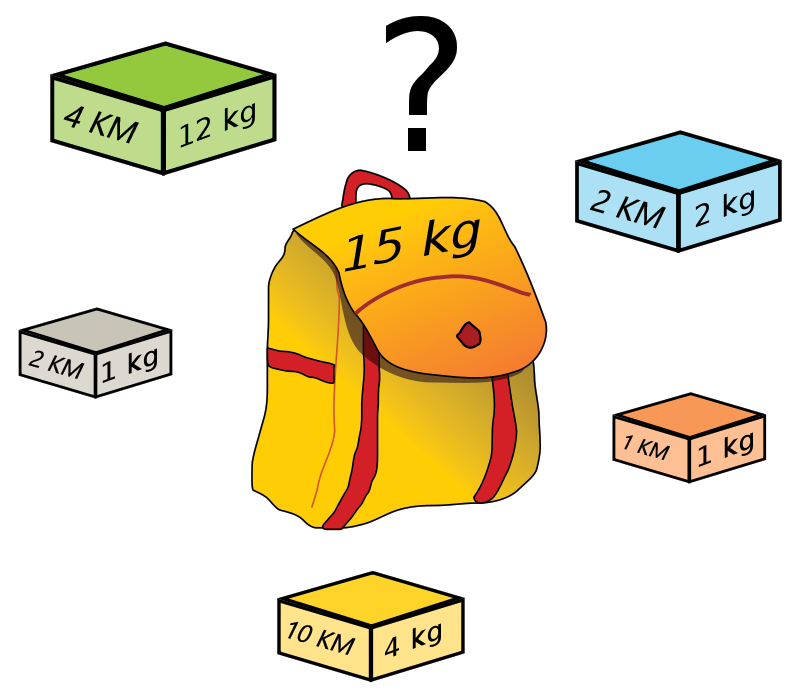
\includegraphics[width=10.4cm, height=9.1cm]{Operations-Management4.png}};
 	\node [ text width=12cm,align=center] at (img.center){ \color{black}	{\bfseries{\huge
 				Uvod u operaciona istraživanja}\\
 		       \vskip 1.5cm
 			\Large Marko Đukanović i Dragan Matić   \\  
 			\vskip 14cm
 			{Univerzitet u Banjoj Luci} \\  
 			Prirodno-matematički fakultet \\
 		%	\vskip 9cm
 			$\the\year{}$.
 		}
};
 \end{tikzpicture}
\newpage
\pagestyle{fancy}
\fancyhead{}
\fancyfoot[C]{\thepage}
%\fancyhead[R]{\thepage}

\fancypagestyle{plain}{%
	\fancyhead{}
	\fancyfoot{}
	\fancyhead[R]{\thepage}
}

\pagenumbering{roman}
\begin{comment}
\begin{titlepage}
	\centering
	\vfill
 
\includegraphics[width=\textwidth]{Operations-Management.jpg}
	{\bfseries{\huge
		Uvod u operaciona istraživanja}\\
		\vskip 1cm
	\large Marko Đukanović  \& Dragan Matić   \\ \vspace{1cm} 
	 
  {Univerzitet u Banjoj Luci} \\ \vspace{5cm}
  $\today$
	}    
	\vfill  \frontmatter
 

	\vfill
	\end{comment}

%\maketitle
 
\newpage
 
\tableofcontents


\newpage
\chapter*{Predgovor}
Ovaj udžbenik je namijenjen studentima koji slušaju uvodni kurs iz Opera\-cionih istraživanja. Po svojoj strukturi i sadržaju udžbenik najviše prati nastavni plan i program za Operaciona istraživanja, za studente treće godine informatičkog smjera Prirodno-matematičkog fakulteta Univerziteta u Banjoj Luci.

Pretpostavljamo da čitaoci ovog udžbenika u dovoljnoj mjeri vladaju solidnim znanjem iz matematike i programiranja, koje uključuje osnovne linearne algebre (manipulacija vektorima i matricama), teorije grafova, kombinatorike, kalkulusa, teorije algoritama i struktura podataka. Za implementaciju programa linearnog programiranja, podrazumijeva se posjedovanje osnovnih programerskih vještina, koje se stiču na uvodnim kursevima iz programiranja, te poznavanje rada u  programskim jezicima C/C++ i/ili Python. 

Cilj ovog udžbenika je da čitaoca upozna kako sa lijepom matematičkom teorijom koja je u osnovi operacionih istraživanja, tako i sa praktičkim problemima, koji se rješavaju primjenom odgovarajućih tehnika. U udžbeniku je prezentovan veliki broj primjera realnih problema koji potiču iz prakse, a na različitim mjestima su objašnjene različite faze rješavanja tih problema, počev od  identifikovanja samog problema, njegove formalne matematičke formulacije, analize  metoda za rješavanje, pa do implementacije rješenja u odgovarajućem rješavaču ili pak pomoću samostalno dizajniranog algoritma. 


Uz pomoć znanja stečenog iz ovog udžbenika, polaznik će biti sposoban da sam identifikuje i formuliše probleme koji spadaju u oblast operacionih istraživanja (sa naglaskom na probleme linearnog i cjelobrojnog programiranja), analizira različite metode za rješavanje datih problema, te, primjenjujući odgovarajuće računarske alate, implementira algoritme i rješava probleme.

Unutar svakog poglavlja prikazan je i značajan broj primjera koji mogu pomoći lakšem razumijevanju gradiva. Neki primjeri su urađeni kompletno, od početka do kraja, dok neki drugi sadrže prikaze koraka koji su klju\v cni za razumijevanje datog koncepta. Treba pomenuti da u modelovanju problema metodama linearnog programiranja, često postoji više podjednako dobrih i efikasnih rješenja. Stoga se od čitaoca ne očekuje da predložena rješenja usvoji kao jedina moguća, već da analizom ponuđenih rješenja i povezivanjem raznih koncepata i tehnika sam dođe do svojih rješenja, koja su podjednako ispravna i efikasna.

Na kraju svakog poglavlja dat je veći broj pitanja i zadataka. Cilj ovih zadataka nije da čitalac samo reprodukuje stečeno znanje, već da sam stekne sposobnost da modeluje i implementira algoritme kojima rješava različite probleme, procjenjuje kvalitet rješenja, pronalazi rješenja za razne probleme, koji, na prvi pogled, nisu u bliskoj vezi sa gradivom iznesenim u udžbeniku.

Mnogi koncepti u operacionim istraživanjima se međusobno prepliću i nadopunjuju. Npr. teorija dualnosti se koristi u dekompozicionim metodama, simpleks metoda se može kombinovati sa drugim metodama za rješavanje problema linearnog i cjelobrojnog linarnog programiranja, a egzaktne i heurističke metode za rješavanje problema često se međusobno kombinuju i objedinjuju u tzv. hibridne metode.
Stoga je preporuka da se ovaj udžbenik ne čita isključivo redom, već da se, čak i mnogo češće nego što je to u tekstu sugerisano, sadržaj više poglavlja izučava u isto vrijeme, vraća na prethodna poglavlja ili prelazi na neka naredna.


Za uspješno savladavanje gradiva iznesenog u udžbeniku potreban je strpljiv i studiozan rad. Čitaocu se preporučuje i da sve prezentovane primjere detaljno razradi i po potrebi testira na svom računaru, da dodatno analizira ponuđena rješenja, formira svoje mišljenje o rješenjima u udžbeniku i predloži svoja rješenja. Neki zadaci podrazumijevaju i dodatni angažman, koji uključuje prikupljanje potrebnih informacija i iz drugih izvora (na primjer iz pouzdanih internet izvora),  što je u praksi standardan i uobičajen metod za učenje i napredovanje u struci.

Na kraju, želimo da se zahvalimo recenzentima, doc. dr Milani Grbić i doc. dr Aleksandru Kartelju, koji su svojim sugestijama i komentarima poboljšali kvalitet ovog udžbenika. Takođe, zahvaljujemo se na podršci i kolegama sa Katedre za računarske i informatičke nauke Prirodno-matematičkog fakulteta Univerziteta u Banjoj Luci.



\chapter*{Notacija}

Uvedimo neke notacijske napomene i konvencije koje smo koristili u knjizi.

\begin{itemize}
	\item Smatraćemo da je vektor uvijek dat u kolonskoj notaciji, tj. 
	$x= \left (\begin{matrix}
		     x_1 \\
		     x_2 \\
		     \vdots\\
		     x_n
	\end{matrix} \right ) \in \mathbb{R}^n,$ dok je njegov odgovarajući transponovani vektor $x^T=(x_1,\ldots, x_n) \in \mathbb{R}^{1\times n}$. 
   \item Što se tiče skalara i vektora, nećemo koristiti drugačije oznake da bismo ih razlikovali. Jednostavno, biće jasno iz konteksta da li je riječ o jednom ili drugom. Dakle, nula vektor ćemo takođe označavati sa $x = (0, \ldots, 0)^T := 0$, dok je $x=(1,\ldots, 1)^T:=1$.  
   \item   Ako je $x \in \mathbb{R}^n$, notacija  $x \geq 0$ podrazumijeva da je vrijednost svake od koordinatna vektora $x$ veća ili jednaka 0, tj. $x_i \geq 0$, za sve $i=1,\ldots,n$. 
\end{itemize} 


\chapter{Predmet izučavanja Operacionih istraživanja}
\pagenumbering{arabic}

Operaciona istraživanja su oblast koja pripada matematičkim disciplinama. Ona predstavlja osnovnu disciplinu u menadžmentu, a naziv joj potiče iz njene osnovne uloge, a to je istraživanje  operacija u organizacionim sistemima (logistika, problem raspoređivanja, dodjeljivanja zadataka itd.) gdje je svrha optimizacija (troškova, vremena, ljudskih resursa, opreme itd.). Operaciona istraživanja u osnovi predstavljaju analitički metod rješavanja problema i donošenja odluka koje se primjenjuju u organizaciji raznih sistema i procesa. Metodologija ovih istraživanja  najčešće obuhvata razbijanje problema na bazne komponente, te potom njihovo rješavanje u definisanim koracima uz pomoć matematičkog aparata. 


Koncept operacionih istraživanja potiče iz vremena Drugog svjetskog rata, gdje su vojni planeri razvijali strategiju postavljanja vojske i vojne opreme sa ciljem što veće mobilnosti i efikasnosti. Od tog vremena, pa sve do danas, tehnike u operacionim istraživanjima se primjenjuju u rješavanju velikog broja problema u poslovnom svijetu, industriji, društvenim pitanjima i mnogim drugim aspektima savremenog društva. 


Proces u operacionom istraživanju se ugrubo može predstaviti sljedećim koracima:
\begin{itemize}
    \item Opisivanje problema koji rješavamo.
    \item Konstrukcija modela problema koji izražava taj problem preko promjenljivih i relacija između njih. 
    \item Korištenje modela za generisanje rješenja problema.
    \item Testiranje svakog od rješenja i analiziranje njihovih  kvaliteta.
    \item Implementacija odabranog rješenja datog problema. 
\end{itemize}

Detaljima ovih koraka ćemo se baviti  u narednoj sekciji.
 

Glavne teme izučavanja operacionih istraživanja su:
\begin{itemize}
     \item \emph{Optimizacija:} %Uloga operacionih istraživanja je   dohvatiti najbolje performanse pod unaprijed zadanim resursima (limit u vremenu, memoriji, itd.). 
       uključuje poređenja i navođenje pretrage prema potencijalno boljim opcijama u okviru zadanih resursa.
     \item \emph{Simulacija}:  podrazumijeva izgradnju modela problema iz koga se dobijaju rješenja, koja se nakon toga provjeravaju prije nego što se implementiraju u realnoj situaciji.
     \item \emph{Vjerovatnoća i statistika}:  podrazumijeva ($i$) upotrebu matematičkih algoritama i podataka u smislu otkrivanja korisnih informacija koje služe za dobijanje pouzdanih predviđanja u realnom svijetu; ($ii$) testiranje kvaliteta i upotrebljivosti rješenja.
\end{itemize}
 
 Operaciona istraživanja imaju nezamjenjivu ulogu u nizu obasti kao što su problemi raspoređivanja, urbanog planiranja, optimizacije na mrežama i inženjeringu, rutiranja paketa, upravljanja rizicima, upravljanja lancem snabdjevanja i mnogim drugim. 

 Operaciona istraživanja rješavaju probleme iz prakse (nazovimo ih poslovni problemi), koji ljudima štede novac i vrijeme. Ovi problemi mogu biti raznoliki i po pravilu ne izgledaju naročito povezani jedni sa drugim. Gledajući šire, osnov  im je uvijek isti, donošenje niza odluka da bi se došlo do cilja na što efikasniji način.
Jedna od najmoćnijih tehnika koje se mogu koristiti u operacionim istraživanjima je \emph{matematičko programiranje}. Treba imati na umu da riječ  ,,programiranje'' nema standardno značenje na koje smo i navikli -- imperativno, vec ono u ovom kontekstu oznacava programiranje optimizacionih modela, koje je u osnovi deklarativno. 

  Put od učenja o problemu kojeg klijent predstavi do pronalaska rješenja može biti jako izazovan. Ovaj proces rješavanja se  dijeli u četiri osnovna nivoa apstrakcije:
  \begin{enumerate}
      \item poslovni problemi;
      \item generički problemi; 
      \item paradigma modelovanja;
      \item algoritamska rješenja. 
  \end{enumerate}
  
 Pod \emph{poslovnim problemima}  se ne podrazumijevaju samo problemi iz domena ekonomije, što samo ime možda nameće, već svi problemi koji imaju primjenu u stvarnom svijetu. Pojam ,,poslovni'' više odgovara tome da problem nema svoju preciznu matematičku formulaciju, već je neformalno definisan kroz jezički (deskriptivan) opis.  Najčešće, ovi problemi proizilaze iz problema u ekonomiji ili industriji i kao takvi se i opisuju. Npr. u neformalnom opisu problema raspoređivanja medicinskog osoblja u (tri) smjene, navode se uslovi poput toga da svaki radnik mora da odradi 40 sati sedmično ili da niti jedan radnik ne smije da radi više od dvije noćne smjene u toku sedmice. Nakon opisnog, neformalnog definisanja, naredni korak 
 je formalno definisanje problema, odnosno, ,,spuštanje'' (opisa) problema na niži nivo apstrakcije. U praksi se ovaj proces odvija iterativno i povezuje se sa terminom \emph{generički problemi}. Npr. problem pravljenja rasporeda časova, koji je poslovni problem, se može prevesti u generički OR problem bojenja grafa.

Na početku razvoja operacionih istraživanja kao naučne discipline nije bilo strogog matematičkog formalizma. Matematičari su prepoznali da se većina poslovnih problema može  preslikati u generičke familije problema nižeg nivoa. Na kraju se završilo sa nekoliko opšteprihvaćenih generičkih klasa na koje se preslikava gotovo svaki poslovni problem. U praksi, najveći dio vremena se provodi u prevođenju poslovnog problema u jedan od tipova generičkih problema. Nakon toga, rješavanje problema je manje-više standardna procedura. Generički problemi operacionih istraživanja su dovoljno koncizni da se mogu predstaviti  matematičkom notacijom. Međutim, u svrhu boljeg razumijevanja, u praksi se koristi jezik modelovanja koji je na višem nivou apstrakcije. Npr. problemi raspoređivanja se obično opisuju upotrebom ,,stvarnih'' termina, kao što su resursi, aktivnosti, prioriteti, uslovi raspoređivanja i sl.  

 \emph{Paradigma modelovanja}. Kod generičkih problema koji su definisani jezikom višeg nivoa, notacija je najčešće vezana za problem koji se razmatra.
 Npr. resursi i aktivnosti nisu nešto što se može definisati u poznatom problemu trgovačkog putnika. U osnovi, svaki od ovih generičkih problema se može opisati nekom od paradigmi modelovanja. Paradigma modelovanja predstavlja skup pravila koja omogućuju da predstavimo probleme višeg nivoa, koristeći strukture nižeg nivoa, kao što su, na primjer, matrice. Kada se primjenjuje ova paradigma, problem se izražava upotrebom matematičke notacije ili algebarskog jezika modelovanja (eng. \emph{Algebraic Modelling Language} (AML)), koji konvertuje matematičku notaciju u matrice koje su proslijeđene sljedećem nivou (\emph{algoritamska rješenja}), koji generiše rješenja. Najpoznatije paradigme modelovanja su sljedeće: \textit{linearno}, \textit{cjelobrojno} i \textit{mješovito-cjelobrojno programiranje}. Postoje i druge paradigme poput modelovanja ograničenjima (eng. \emph{constraint programming}) i mrežnog modelovanja (eng. \emph{network models}). 

 \emph{Algoritamska rješenja}.   Algoritam je konačan niz instrukcija čijim izvršavanjem možemo riješiti problem ili njegov dio. Neki algoritmi su opšti, kao, na primjer, sortiranje ili pretraživanje,  dok su drugi vezani uz specifične probleme. Algoritmi pretrage su izuzetno važni u rješavanju problema operacionih istraživanja. Među njima se izdvajaju ,,Branch \& X''-tip algoritama koji rješavaju Cjelobrojne, Mješovito-cjelobrojne probleme kao i probleme zasnovane na modelovanju ograničenjima. Među ove algoritme spadaju Branch \& Bound (za rješavanje problema cjelobrojnog programiranja), Branch \& Cut, Branch \& Price (tj. metod generisanja kolona), itd.

\emph{Dinamičko programiranje} je još jedna značajna programska paradigma  koja se primjenjuje za rješavanje problema u oblasti operacionih istraživanja. Ova familija algoritama rješava probleme tako što eksploatiše optimalnu pod-strukturu problema. Drugim riječima, polazni problem razbijemo na manje podprobleme, koje rješavamo rekurzivno. U rješavanju glavnog problema, koristimo pronađena optimalna rješenja podproblema, izbjegavajući ponovno rješavanje podproblema koji su već jednom bili rješavani. Ova programska paradigma ima značajnu ulogu u rješavanju grafovskih problema. 
%Jedan od najpoznatijih takvih algoritama je \emph{Bellman-Ford}-ov algoritam, nazvan po izumitelju  paradigme dinamičkog programiranja, Ričardu Belmanu. 

U praksi, problemi iz oblasti operacionih istraživanja mogu biti prilično teški za egzaktno rješavanje, što podrazumijeva da je za dobijanje optimalnog rješenja potrebno jako puno vremenskih i memorijskih resursa. Za potrebe dobijanja brzog (ne obavezno optimalnog) rješenja  koriste se \emph{pohlepni algoritmi}. Oni obično ne mogu 
da garantuju optimalnost, ali su   po svojoj prirodi jako brzi u nalaženju dovoljno dobrog rješenja. Jedan od najpoznatijih pohlepnih algoritama je \emph{Dajkstrin} algoritam za problem pronalaska najkraćeg puta koji, pri određenim uslovima, nalazi i optimalno rješenje. 

 \begin{figure}
    \centering 
    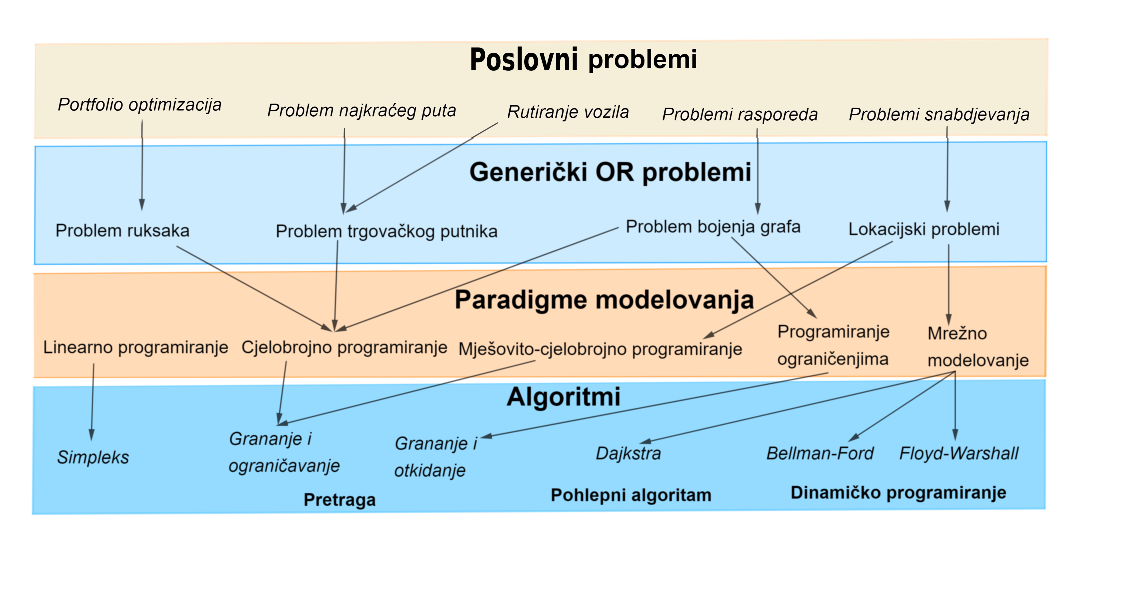
\includegraphics[width=\textwidth,height=250pt]{overview.eps}
    \caption{Četiri nivoa apstrakcije pri rješavanu problema operacionih istraživanja.}
    \label{fig:OR_four_levels}
\end{figure} 
%https://towardsdatascience.com/the-big-picture-of-operations-research-8652d5153aad


U nastavku ćemo detaljno objasniti svaki od nivoa apstrakcije u operacionim istraživanjima, najvažnije paradigme modelovanja i najznačajnije algoritme za rješavanje navedenih problema. Odnosi između sva četiri nivoa apstrakcije su dati na Slici~\ref{fig:OR_four_levels}. 
 Na kraju knjige će biti riječi o opštem rješavaču, koji je u savremenoj parksi jedan od standardnih alata za rješavanje problema iz oblasti operacionih istraživanja.
 
  
\chapter{Principi modelovanja u Operacionim istraživanjima}
Uobičajeno je izraz Operaciona istraživanja zapisivati akronimom OR (eng. \emph{operations research}). 
U ovoj glavi ćemo objasniti   glavne faze tipičnog OR-a, koje se realizuje u  komercijalne svrhe. Faze OR-a možemo sumirati u sljedeće (preklapajuće) faze: 
 \begin{itemize}
     \item Definisanje problema i sakupljanje relevantnih podataka.
     \item Formulisanje matematičkog modela datog problema.
     \item Razvoj računarske procedure koja će pronaći rješenja datog problema na osnovu modela.
     \item Testiranje modela i, po potrebi, rad na njegovom poboljšanju.
     \item Pripremu za primjenu modela, kako je definisano od strane korisnika koji naručuje/finansira sistem baziran na OR.
     \item Implementaciju i upotrebu rješenja.
 \end{itemize}
  U nastavku ćemo opisati svaku od ovih faza.
 
  \section{Definisanje problema i sakupljanje relevantnih podataka}
 
 Većina praktičnih problema, sa kojima se susrećemo  su u početku opisani na neprecizan način. Stoga, prvi zadatak podrazumijeva dobro definisanje  cilja/namjene  (eng. \emph{objectives}) samog zadatka koji treba riješiti, uslova pod kojim je rješenje problema validno,  vremenskih ograničenja za donošenje odluka i moguće alternativne scenarije.  Definisanje problema na dovoljno dobar način je značajan korak, jer uveliko utiče na relevantnost zaključaka istraživanja. Izvlačenje odgovora ili dobijanje rezultata iz pogrešne postavke polaznog problema gotovo sigurno neće dovesti do ispravnog rješenja.  

 Zbog toga je važno da osoba (ili više osoba) koja modeluje problem,  ne radi samostalno, već blisko sarađuje sa poslodavcem. Osoba koja je zadužena za formulisanje problema, savjetuje se sa poslodavcem za koga se razvija sistem, poslije čega se izrađuje detaljna tehnička analiza u vezi problema i izlažu preporuke za rješenje  poslodavcu, koji je ključan u donošenju odluka.   


 Izvještaj koji se predaje poslodavcu, najčešće sadrži osnovno rješenje, ali i brojne alternative koje odgovaraju različitim uslovima ili  vrijednostima parametara problema  (npr. balansiranje između cijene i dobiti, stabilnosti poslovanja i dobiti/profita, itd.). Na poslodavcu je da vrednuje prijedloge, uzimajući u obzir  niz faktora, nakon čega se donosi odluka zasnovanu na najboljoj procjeni. %Važno je da osoba zadužena za izradu rješenja bude sličnog mišljenja kao i naručilac. %Utvrđivanje odgovarajućih ciljeva je  neophodno za ispravno   definisanje problema.   Zato je potrebna neprestana komunikacija sa poslodavcem, koja je donosilac odluka u vezi sistema koji se razvija, da bi se što prije pristupilo  realizaciji svakog od ciljeva.


  OR istraživanje podrazumijevano traži  ona rješenja koja su optimalna, ali se optimalnost može odnositi samo za određenu komponentu procesa za koji se sistem razvija. Prema tome, ciljevi koji su formulisani bi trebali da traže optimalna rješenja čitavog procesa koji se optimizuje.  U praksi, ovakav zahtjev nije trivijalan, te se problem svodi na razmatranje dijela inicijalno definisanog problema (ili njegove pojednostavljene varijante). Drugim riječima, analiza bi mogla postati pretjerano glomazna ako bi zadani ciljevi bili previše uopšteni. Umjesto toga, ciljevi bi trebalo da budu specifični, koliko god je to moguće, ali da se pri tome obuhvate glavni ciljevi donosilaca odluka. 


 Jedan od mogućih pristupa zaobilaženja problema pod-optimizacije je korištenje dugoročne maksimizacije nekog cilja, npr. profita. Riječ ,,dugoročno'' ukazuje da cilj pruža fleksibilnost u razmatranju aktivnosti koje ne donose momentalnu dobit, ali   omogućuju krajnji profit. Ovakav cilj je dovoljno specifičan, a ipak i dovoljno širok da obuhvati osnovni cilj   organizacija, dolazak do (zadovoljavajuće) zarade. Zapravo, svi drugi legitimni ciljevi ovakvih organizacija mogu se podvesti u prethodno pomenuti. Međutim, u praksi   organizacije rijetko koriste ovaj pristup. Velik broj   organizacija prilagođava zadovoljavajući profit sa drugim ciljevima, umjesto fokusiranja na maksimizovanje dugoročne zarade. Neki od takvih ciljeva su: izgradnja stabilnog profita, povećanje udjela na tržištu, zadržavanje stabilnosti cijena, povećanje uticaja kompanije, povećanje ponude proizvoda, itd. 
 Dalje, treba napomenuti i dodatna razmatranja, poput društvenih odgovornosti, koje nisu direktno motivisane profitom.  

 Postoji nekoliko strana kojih se direktno tiču poslovi firme: (1) vlasnici (dioničari, itd.), koji žele profit;   (2) zaposlenici koji žele stalno zaposlenje, stabilan posao, te razumne plate; (3) kupci koji žele proizvod zadovoljavajućeg kvaliteta po razumnoj cijeni;
 (4) dobavljači, koji žele integritet i razumnu prodajnu cijenu proizvoda; i
 (5) vlada, koja želi plaćanje poreza i razmjenu dobara. Sve ove strane na određeni način utiču na poslovanje firme, ali i obrnuto.  Stoga, dok je glavna odgovornost uprave profit (što, na kraju krajeva, koristi svim stranama), napomenimo da se treba sagledati i širi društveni uticaj ovakvog procesa. 
 
  Osobe zadužene za modelovanje obično provode dosta vremena prikupljajući relevantne podatke o problemu. Potrebno je prikupiti mnogo podataka kako bi se došlo do razumijevanja problema i dolaska do potrebnih ulaznih podataka matematičkog modela, koji se konstruiše u narednoj fazi.  Mnogi podaci često nisu dostupni, bilo zbog toga što informacije nikada nisu sačuvane ili su zastarjele ili su pak sačuvane u neočekivanim formatima. Potrebno je komunicirati sa poslodavcem, kako bi pronašli sve podatke značajne za projekat. Međutim, dio podataka mogu biti prilično ,,neprecizan'', tj. to su grube procjene zasnovane na iskustvenim pretpostavkama. Tada je neophodno izdvojiti značajnu količinu vremena za poboljšanje  
 preciznosti podataka, da bi se proces nastavio sa najboljim mogućim resursima i smanjila mogućnost pravljenja grešaka. 

  \begin{primjer}
  OR studija je urađena za policijsku upravu jednog grada %San Francisca 
 za razvoj računarskog sistema za optimalno raspoređivanje i postavljanje patrolnih službenika. U procjeni   ove studije, identifikovani su sljedeći glavni ciljevi:
 \begin{enumerate}
     \item  Održavati visok nivo sigurnosti građana.
     \item  Održavati visok nivo zadovoljstva u policiji.
      \item Minimizovati troškove operacija.
 \end{enumerate}
 Da bi se postigao prvi cilj, policijska uprava i gradska vlada  su zajednički radili na uspostavljanju željenog nivoa zaštite.  Matematički model je razvijen na način da se postizanje potrebnog nivoa zaštite realizuje pomoću funkcije cilja.  Da bi se postigao drugi cilj, u samom modelu je uključen i uslov o ravnomjerno raspoređenim radnim satima među policajcima. Treći cilj je ugrađen u model usvajanjem dugoročnog cilja smanjenja broja policajaca potrebnih za postizanje prva dva cilja. 
 \end{primjer}
 \section{Proces formulisanja matematičkog modela}

 Nakon što se definiše problem odlučivanja, sljedeća faza je formulisanje tog problema u obliku koji je odgovarajući za dalju analizu. Uobičajeni OR pristup se sastoji od konstrukcije matematičkog modela koji na najbolji način odgovara realnom problemu. Prije nego što objasnimo opšti proces konstruisanja takvog modela, recimo nešto o modelima uopšte, a posebno o matematičkim modelima.

  U izvornom značenju, 
 model je oblik (može biti i prikaz, tip ili ponašanje) koji se uzima za primjer, koji se oponaša ili na koji se neko ugleda.  Model se može definisati i kao uzorak po kojem se izrađuje neki proizvod. U svakodnevnom životu se veoma često susrećemo sa različitim modelima.  Tipični primjeri uključuju model aviona, ljudskog lica (portret), zemaljske kugle (globus) itd. Slično tome, modeli igraju
 važnu ulogu u nauci i poslovanju, što uključuje modele atoma, modele 
 genetskih struktura, matematičke jednačine koje opisuju fizičke zakone kretanja, grafikoni, itd. Takvi modeli
 su od neprocjenjive važnosti za apstraktno poimanje suštine predmeta istraživanja, ukazivanja na međusobnu interakciju pojava i olakšavanja kompleksnih analiza. 

 Matematički model je približni opis nekih pojava ili objekata u stvarnom svijetu, uz pomoć matematičke simbolike (funkcija, jednačina itd.). Npr. drugi Njutnov zakon se matematički modeluje poznatom formulom $F=ma$. Matematički model poslovnih problema   
 se sastoji od sistema jednačina i matematičkih izraza koji opisuju osnov problema. Npr. postoji $n$ mjerljivih odluka koje treba odrediti, a koje su predstavljene pomoću nepoznatih promjenjljivih $x_1,\ldots, x_n$.  Odgovarajuća mjera učinka (profita) je izražena preko matematičkih funkcija nepoznatih koje odgovaraju  odlukama ($3x_1 + 5x_2 + x_3$). Ova funkcija se naziva \emph{ciljna} (objektivna) funkcija, ili \emph{funkcija cilja}. Ograničenja  vrijednosti promjenjivih se takođe izražavaju matematičkim izrazima, (npr. $x_1 + x_2 + x_3 \leq 1$).  Ovakvi matematički izrazi za ograničenja se tako i nazivaju -- \emph{ograničenja} (eng. \emph{constraints}). Konstante u ograničenjima, te u ciljnoj funkciji, se nazivaju \emph{parametri} modela.

 Prema tome, rješavanje matematičkog modela 
 podrazumijeva izbor vrijednosti promjenljivih odlučivanja, tako da se maksimizuje/minimizuje vrijednost funkcije cilja u odnosu na određena ograničenja. Takvi modeli, sa manjim varijacijama, karakterišu i modele koji su prisutni u OR oblasti. 
 Određivanje odgovarajućih vrijednosti, koje se dodjeljuju parametrima modela, je kritični dio procesa konstrukcije modela.

 Za razliku od problema iz udžbenika, za koje su ove vrijednosti unaprijed poznate,   određivanje parametara u stvarnim situacijama najprije zahtijeva prikupljanje relevantnih podataka. Kao što je objašnjeno u prethodnoj sekciji,  prikupljanje tačnih podataka je veoma izazovan proces. Dodijeljena vrijednost parametru često predstavlja  samo grubu procjenu stvarne situacije. Zbog nepouzdanosti vrijednosti parametara, važno je analizirati kako se rješenje, koje je izvedeno iz modela, mijenja pri malim promjenama vrijednosti parametara. 
  Problemi iz prakse obično nemaju samo jedan ,,ispravan'' model. Često   dva ili više   različito formulisana modela mogu da odgovaraju jednom problemu. 
 Ovo je stvar razvoja modela koji je iterativni proces koji proizilazi iz rezultata testiranja i potrebe za konstrukcijom boljeg modela.

  Postoji i nepisano pravilo da nijedan matematički model koji opisuje realnu situaciju nije potpuno tačan, pa je cilj konstruisati onaj model koji,  što je moguće preciznije, opisuje tu realnu situaciju.


  U nastavku  ćemo vidjeti brojne primjere matematičkih modela. Jedna posebno važna vrsta modela koju proučavamo u sljedećih nekoliko poglavlja
 je model linearnog programiranja, gdje su i ciljna funkcija i ograničenja zadati linearnim funkcijama. 
  Matematički modeli imaju još jednu prednost u odnosu na jezički opis problema -- problem se opisuje mnogo sažetije. Na taj način, cjelokupna struktura problema je razumljivija, a otkrivanje važnih uzročno-posljedičnih veza u samom problemu je dosta lakše. Takođe, matematički
  model čini most za primjenu moćnih matematičkih tehnika i računara u
 analizi i rješavanju problema. Zapravo, računarski programi za rješavanje raznih tipova modela su  u današnje vrijeme  široko dostupni (na primjer, poznati rješavači kao što su \textsc{Cplex}, Gurobi, Lindo itd.). 

  Postoje i ,,zamke'', na koje treba paziti, kada koristimo matematičke modele. Ako želimo da, na kraju, formirani model bude upotrebljiv za rješavanje problema, često  su neophodne aproksimacije i pojednostavljivanja pretpostavki. Stoga se mora paziti da model ostane valjan prikaz problema nakon primjene svih pojednostavljenja. To znači da treba da postoji značajna korelacija između onoga što model predviđa i onoga što bi se zapravo i dobija primjenom modela u stvarnoj situaciji. Da bi se utvrdilo da li je ovaj zahtjev zadovoljen, potrebno je izvršiti značajna ispitivanja i posljedične izmjene u inicijalnom modelu. O ovome ćemo govoriti u narednim sekcijama. U osnovi, provjera valjanosti modela zapravo se provodi tokom svih  faza izrade modela. 
  
  Preporučljiv pristup u razvoju modela je da se započne sa pojednostavljenom verzijom, a  evolucionim načinom ići prema složenijim modelima, koji će bolje odražavati  stvarni problem. Ovaj proces obogaćivanja modela se nastavlja dok god je model rješiv. Kompromis, kojeg se pridržavamo, je odnos između preciznosti modela i mogućnosti njegovog rješavanja. Ključni korak u razvoju modela je konstrukcija funkcije cilja.
 On podrazumijeva razvijanje kvantitativne mjere uspješnosti u odnosu na svaki krajnji cilj, koji je identifikovan tokom definisanja problema.
 Ako postoji više ciljeva, njihove se mjere obično transformišu
i kombinuju u jednu složenu mjeru -- ali postoje i pristupi koji nezavisno analiziraju funkcije cija, tzv. visekriterijumska optimizacija.    Ukupna mjera može biti nešto opipljivo (npr. dobit), što odgovara višem cilju
 organizacije.  Nakon što se razvije cjelokupna mjera,  ciljna funkcija se izražava kao matematička funkcija čiji su argumenti promjenljive odlučivanja. 

% primjer preuzet iz: http://www.mathos.unios.hr/~mdjumic/uploads/diplomski/ČOR03.pdf
 \begin{primjer}
 Uzmimo jednog proizvođača negaziranih pića. On pravi dvije vrste soka: multivitaminski gusti i multivitaminski bistri sok, od sastojaka $A$ i $B$, te vode. Da bi se napravilo 100$l$ multivitaminskog gustog soka potrebno je 3$l$
 sastojka $A$ i 8$l$ sastojka $B$, a za bistri sok je potrebno 6$l$ sastojka $A$ i 4$l$ sastojka $B$. Sto litara gustog soka nosi zaradu od 100KM, a 100$l$ bistrog zaradu od 125KM. Proizvođač u skladištu
 ima na raspolaganju 30$l$ sastojka $A$ i 44$l$ sastojka $B.$ Napravljene sokove sipa u burad. Za
 gusti sok ima bure u koje stane 500$l$, a za bistri sok bure kapaciteta 400$l$.  Cilj proizvođača sokova je odrediti količinu soka kojeg treba napraviti da bi se  maksimizovala profit,  uzimajući u obzir data ograničenja. Drugim
 riječima, treba konstruisati plan proizvodnje u cilju maksimizacije profita.
	
 \end{primjer}
 Model za ovaj problem bi se mogao konstruisati na sljedeći način:
 \begin{itemize}
     \item 
Promjenljive odlučivanja: $x_1$ i $x_2$ koje označavaju koliko stotina litara gustog soka i koliko litara bistrog soka proizvođač treba da napravi, respektivno.  
\item Funkcija cilja: $f(x_1, x_2) = c_1x_1 + c_2 x_2$, gdje su $c_1 = 100$ i  $c_2 = 125$ koeficijenti. Funkciju $f$ treba maksimizovati. 
\item Ograničenja: $0 \leq x_1 \leq 5, 0 \leq x_2 \leq 4$,   $3 x_1 + 6 x_2 \leq 30$ i $8 x_1 + 4 x_2 \leq 44.$
\end{itemize}
Prva dva ograničenja se odnose na kapacitet buradi za smještanje gustog, odnosnog bistrog soka. Preostala dva ograničenja su vezana za količinu raspoloživih resursa, odnosno sastojaka $A$ i $B$, potrebnih za proizvodnju sokova.

U narednim poglavljima knjige ćemo detaljno razmatrati postupke kako se dolazi do rješenja ovakvih modela.
 


\section{Izvođenje rješenja iz modela}


Nakon formulacije matematičkog modela za definisani problem, sljedeća faza u OR procesu  je razvoj postupka (algoritma) za
izvođenje rješenja na osnovu konstruisanog modela. Nekada je to relativno jednostavan korak, u kojem se na računaru izvršava neki od standardnih algoritama u okviru odgovarajućih računarskih paketa/rješavača matematičkog modela. Sa druge strane, nekada su matematički modeli toliko složeni da se ne mogu riješiti direktnom primjenom standardnih algoritama, već se podrazumijeva razvoj i primjena drugih, sofisticiranih tehnika.
Nakon dobijanja rezultata, potrebno ih je analizirati. Postupak analize rezultata ćemo, takođe, objasniti u nastavku udžbenika. 

Uobičajeni zadatak u OR oblasti je potraga za optimalnim (najboljim) rješenjem i razvoj odgovarajućih postupaka koji služe za pronala\-ženje optimalnih rješenja zadatog modela. Treba imati na umu da su ta rješenja optimalna samo za dati model. Kako model ne mora da u potpunosti odgovara stvarnom problemu, ne postoji garancija da će se pronađeno optimalno rješenje modela pokazati i najboljim mogućim rješenjem za stvarni problem koji se razmatra. Međutim, ako je
model dobro formulisan i testiran, rezultujuće rješenje  bi trebalo da bude prihvatljivo. U praksi se često pokaže da je ,,dovoljno dobro'' rješenje čak prihvatljivije nego trošenje nerazumno mnogo vremena za traženje optimalnog.    

Najčešće se prvo postavi lista zahtjeva, koje dati model treba da ispuni, a rješenje, koje zadovoljava te uslove (zahtjeve), najčešće se   uzima kao prihvatljivo. U procesu donošenja odluka, pokušava se što više  koristiti naučni pristup, sa primarnim ciljem pronalaska globalnog optimuma za posmatrani model. Međutim,  uslov da se u razumnom vremenu dođe do modela koji generiše rješenje  zadovoljavajućeg kvaliteta, najčešće ima prednost u odnosu na pronalazak optimuma u nerealno dugom vremenskom roku. Osoba koja rukovodi procesom treba da razmotri troškove procesa razvoja modela, a zatim
pokuša da maksimizuje korist u oba smjera. Povremeno se koriste   približni (heuristički) pristupi rješavanju problema. Ovakvi pristupi su intuitivno dizajnirani postupci kojima se ne garantuje dobijanje optimalnog rješenja. Posljednjih nekoliko decenija postignut je velik napredak u razvoju efiksanih heurističkih postupaka (uključujući tzv. metaheuristike o kojima će više biti riječi u Glavi~\ref{chp:heuristike}), a njihova upotreba u ovom polju iz dana u dan sve više dobija na značaju.  

Kao što je već nekoliko puta pomenuto,  i optimalno rješenje za konstruisani model može biti daleko od idealnog za stvarni problem, pa su potrebne dodatne analize. Stoga je analiza ,,postoptimalnosti'' (analiza provedena nakon pronalaska optimalnog rješenja) vrlo važan dio OR studija.  Ova analiza se ponekad naziva i \emph{šta--ako analiza} (eng. what-if analysis), jer uključuje postavljanje pitanja o tome što bi bilo sa optimalnim rješenjem ako se uvedu različite pretpostavke, što implicira dodavanje novih ograničenja u postojeći model. Ova pitanja često postavlja poslodavac koji donosi konačne odluke u vezi procesa dodavanja uslova.  

Pojava softvera koji rade sa proračunskim tabelama (prvenstveno Excel-a) odigralo je centralnu ulogu u provođenju analize postoptimalnosti. Jedna od velikih prednosti ovakvih softvera je jednostavnost u korišćenju, gdje se lako dobija analiza šta se događa sa optimalnim rješenjem kada se naprave promjene na modelu.  Ovakva eksperimentisanja sa promjenama u modelu mogu biti od velike pomoći u razumijevanju ponašanja samog modela i uvjeravanja u njegovu valjanost.  Analiza postoptimalnosti dijelom  uključuje provođenje analize osjetljivosti, radi utvrđivanja koji parametri modela su najkritičniji (,,osjetljivi parametri'') u određivanju rješenja. Uobičajena definicija osjetljivog parametra je sljedeća:

\emph{Osjetljivi parametri matematičkog modela su oni parametri čija (čak i mala) promjena direktno utiče na promjenu optimalnog rješenja}.


Prepoznavanjem osjetljivih parametara pronalazimo one parametre čija se vrijednost mora odrediti sa posebnom pažnjom, kako bi se izbjeglo narušavanje rezultata modela. Da napomenemo, vrijednost koja se dodjeljuje parametru obično predstavlja samo procjenu neke veličine
(npr. jedinična dobit ili vrijeme potrebno da se neka aktivnost izvrši) čija će vrijednost postati preciznija tek nakon što se rješenje primijeni na (stvarni) problem. Stoga, nakon što se identifikuju osjetljivi parametri, posebna pažnja se posvećuje bližoj procjeni svakog parametra, te  rasponu njihovih mogućih vrijednosti.  U nekim slučajevima, određeni parametri modela predstavljaju interesne odluke (npr. dodjele resursa). Ako je to slučaj, često postoji određena fleksibilnost u vrijednostima koje se dodjeljuju ovakvim parametrima u smislu da se neke vrijednosti povećavaju smanjenjem drugih. Postoptimalna analiza uključuje i istraživanje takvih kompromisa. Analiza postoptimalnosti takođe uključuje i dobijanje niza rješenja koji aktivira niz poboljšanja u modelu i konvergenciju prema idealnom modelu. Postupak poboljšanja modela se nastavlja sve dok    poboljšanja u sljedećim rješenjima ne postanu zanemariva da bi se nastavilo sa ovakvim iterativnim procesom.   Alternativna rješenja (rješenja koja su optimalna za jedan od nekoliko približnih modela) se takođe mogu predstaviti poslodavcu za konačan odabir. 

%\textbf{Primjer.}  Posmatrajmo OR studiju o nacionalnom upravljanja vodama.


\section{Testiranje modela}
 
Razvoj velikih matematičkih modela je analogan razvoju velikih softvera. U praksi se često dešava da se, po završetku izrade prve verzije softvera, javi i određen broj grešaka (bagova). Zbog toga se pristupa raznim procedurama testiranja proizvoda, kako bi se pokušalo pronaći i
ispraviti što više grešaka. Na kraju, nakon niza iteracija poboljšanja programa, programeri mogu da zaključe da trenutni program sada generalno daje  valjane rezultate sa velikom sigurnošću. Može se desiti da neke manje greške ostanu skrivene u programu, te se možda   nikada i neće ukloniti. Slično tome, prva verzija matematičkog modela problema neizbježno sadrži određene
nedostatke. Neki relevantni faktori ili međusobni odnosi i zavisnosti između elemenata modela često ne budu  ispravno ugrađeni
u model, a neki parametri ne budu pravilno procijenjeni. Iako su nepoželjne, ove pojave ne treba shvatati kao fatalne greške, već kao očekivanu pojavu. One mogu biti uzrokovane problemima u komunikaciji, izazovima u razumijevanja svih aspekata problema, te poteškoćama pri prikupljanju pouzdanih podataka. Stoga, prije nego što upotrijebimo model, on se mora  temeljno testirati kako bismo mogli  identifikovati 
i ispraviti što više njegovih nedostataka.  Ovaj postupak ispitivanja i poboljšanja modela radi povećanja njegove valjanosti se naziva \emph{validacija modela}. 

Budući da osobe koje razvijaju model mogu provesti mjesece na izradi svih njegovih detalja, može se desiti i da dođe do odstupanja od suštine modela. Stoga, nakon što su detalji uključeni u 
početnu verziju modela, dobar način za početak provjere valjanosti je ponovni pogled na cjelokupni model kako bi se provjerilo da li model sadrži  očigledne greške i propuste. U cilju što objektivnijeg pristupa, poželjno je da grupa koja radi ovaj pregled uključi barem jednog pojedinca koji nije učestvovao u konstrukciji modela. Preispitivanje definicije
problema i poređenje sa modelom mogu pomoći u otkrivanju nekih  grešaka.  Ponekad se  dodatni uvid u valjanost modela dobija i 
mijenjanjem vrijednosti parametara i/ili promjenljivih odlučivanja, kao i provjerom da li se  izlaz iz modela ponaša na očekivan način. To se često može otkriti kada se parametrima ili promjenljivima dodjeljuju ekstremne vrijednosti u blizini njihovih maksimuma ili minimuma (takozvani ,,korner slučajevi'' -- eng. \textit{corner cases}). 

Sistematski pristup u ispitivanju modela podrazumijeva upotrebu retrospektivnog testa. Ovaj test uključuje upotrebu istorijskih podataka koji prate konstrukciju modela, a zatim procjenjuje koliko bi dobro  model i rezultujuće rješenje funkcionisali, ako bi ono  bilo korišteno u praksi.  Ovaj pristup može da ukaže na dijelove modela koji sadrži određene nedostatatke, što bi dalje zahtijevalo dodatne izmjene i poboljšanja. 
Sa druge strane, nedostatak retrospektivnog testa je taj što koristi iste podatke kao i oni koji su korišteni za formulaciju modela. %Ključno je pitanje da li prošlost zaista reprezentuje budućnost. %Da bi se zaobišao   nedostatak retrospektivnog testiranja, ponekad je korisno privremeno nastaviti sa statusom quo. To će dati nove podatke koji nisu bili dostupni kada  je
%model konstruiran. 
Važno je još dokumentovati postupke testiranja valjanosti modela. Ovo može  povećati povjerenje budućih klijenata u model. Takođe, ako se u budućem vremenu pojave pitanja u vezi sa modelom, ova dokumentacija će  biti korisna prilikom otkrivanja potencijalnih problema. 

\begin{comment}
\textbf{Primjer.}  Primjer se odnosi na OR studiju provedenu   za IBM kako bi se integrisala nacionalna mreža zaliha rezervnih dijelova radi poboljšanja servisne podrške za IBM-ove kupce.

Ovom studijom je dobijen  novi inventarni sistem koji je poboljšao korisničku uslugu kroz koju se uštedilo dodatnih 20 milijuna USD po godini kroz poboljšanu operativnu efikasnost. Posebno zanimljiv aspekt faze provjere validnosti modela ove studije bio je način na koji su  budući korisnici inventarnog sistema ugrađeni u postupak ispitivanja. Prvo su odabrani predstavnici koji su činili korisnički tim čija je uloga bila  savjetovati OR tim. Nakon što je razvijena preliminarna verzija novog sistema izvršeno je njgovo testiranje. Opsežne povratne informacije korisničkog tima dovele su do glavnih poboljšanja u predloženom sistemu.  
\end{comment}

\section{Pripremanje modela za primjenu}
 
 Ako želimo da model bude upotrijebljen više puta u praksi, sljedeći  korak je instaliranje dobro dokumentovanog sistema za primjenu modela po propisima poslodavca. Ovaj sistem uključuje implementaciju samog modela, postupak dobijanja rješenja (uključujući analizu postoptimalnosti), operativne postupke za izvođenje, itd. %Tada, čak i kad se osoblje mijenja, sistem se može pozvati na regularnoj bazi da se ponudi određeno numeričko rješenje
 Svaki put pri korištenju sistema, baze podataka i informacioni sistem za upravljanje treba da omoguće unos podataka u model, te je zbog toga potrebno obezbijediti i odgovarajući interfejs. Nakon što se na model primijeni postupak rješavanja, dodatni  programi mogu automatski pokrenuti implementaciju rezultata kako bi ih korisnici mogli odmah primijeniti u realnoj situaciji. U drugim slučajevima, može se instalirati i interaktivni računarski sistem  za podršku odlučivanju, koji pomaže poslodavcu da koristi podatke i modele kako bi, po potrebi, podržao (ali ne i zamijenio)   donošenje odluka. Dodatna programska rješenja mogu generisati menadžerske izvještaje, koji pomažu pri tumačenju izlaznih podataka modela, kao i implikacije na primjenu u realnom okruženju.  U velikim OR studijama potrebno je nekoliko mjeseci (a nekada čak i duže) za razvoj, testiranje i instaliranje ovakvog računarskog sistema. Pri tome, treba uzeti u obzir da ove aktivnosti uključuju i razvoj i izvođenje postupka održavanja sistema  tokom njegove buduće upotrebe. Kako se uslovi obično mijenjaju tokom vremena, potrebno je obezbijediti i mogućnost za  izmjene sistema, uključujući i izmjene samog modela, u skladu sa tim uslovima.  

 Sljedeći primjer nam opisuje sistem u IBM-u za kontrolu usluga i zaliha rezervi da bi se dobio osjećaj o kompleksnosti ovakvih sistema zasnovaom na OR studiju. 

 \begin{primjer}\label{primjer:IMBOptimizer}
 %OR studija  za IBM predstavljena na kraju prošle sekcije je primjer   velikog sistema koji integriše model.
 Sistem nazvan \emph{Optimizer} pruža optimalnu kontrolu usluga i zaliha rezervnih dijelova u cijeloj IBM-ovoj mreži za distribuciju dijelova u SAD-u. Ona uključuje dva središnja
 automatizovana skladišta, desetine terenskih distribucijskih centara i stanica za dijelove, te nekoliko hiljada vanjskih (povezanih) lokacija. Vrijednost inventara dijelova koji se održava u ovoj mreži se procijenjuje u milijardama dolara. \emph{Optimizer} se sastoji od četiri glavna modula. Modul sistema predviđanja sadrži nekoliko programa za procjenu stope kvara pojedinih vrsta dijelova. Modul sistema za dostavljanje podataka sastoji se od otprilike 100 programa koji    obrađuju
 preko 15 GB podataka kako bi se osigurali ulazni podaci za model. Sistem odlučivanja potom rješava model kako bi se optimizovala kontrola zaliha. Rješavanje ovog modela može da traje i po sedmicu dana. Četvrti modul uključuje šest programa koji integrišu \emph{Optimizer} u IBM-ov sistem upravljanja zalihama dijelova. %PIMS je sofisticirani informacijski i kontrolni sustav koji sadrži milijune redaka koda
  \end{primjer} 

 \section{Implementacija}

 Nakon što se razvije sistem za primjenu modela, posljednja faza  podrazumijeva upotrebu ovog sistema  na način kako je to propisao poslodavac, kao naručilac ovakvog sistema. Ova faza je ključna jer se ovdje ,,ubiru plodovi rada'' sa obje strane. Stoga je važno da osobe zadužene za izradu sistema  učestvuju u  realizaciji ove faze, kako bi se osiguralo da se rješenja modela precizno prevedu u operativni postupak, ali i da bi se otkrili i ispravili svi nedostaci dobijenih rješenja. Uspjeh faze implementacije uveliko zavisi i od podrške poslodavca i uprave. Više je vjerovatno da će osobe uključene u razvoj sistema dobiti podršku ako su dobro informisli poslodavca i podsticli njegovo aktivno učestvovanje tokom razvoja rješenja; dobra komunikacija pomaže da istraživanje postigne ono što je poslodavac i želieo.  Faza implementacije uključuje nekoliko koraka. Prvo,  operativnom rukovodstvu se daje opis novog sistema koji treba da bude usvojen za korištenje. Dalje, obje strane, i poslodavac i razvojni tim, dijele odgovornost za razvijanje koraka potrebnih za pokretanje sistema. Operativno rukovodstvo zatim nadgleda  osoblje koje je uključeno u proces implementacije, te mu daje detaljna uputstva za korištenje sistema. Time počinje proces primjene sistema u realnim uslovima. Nakon uspješnog uvođenja sistema, očekuje se njegovo aktivno korištenje u narednom periodu. Imajući to na umu, određene osobe iz razvojnog tima treba da nadgledaju iskustva korisnika sistema radi utvrđivanja koje izmjene u budućnosti bi trebalo uraditi u sklopu  sistema u cilju njegovog lakšeg korištenja.  Tokom vremenskog perioda u kojem se koristi novi sistem, važno je i dalje dobijati povratne informacije o funkcionisanju sistema, te provjeravati da li su pretpostavke o modelu i dalje zadovoljene. Kada se pojave značajna odstupanja od originalnih pretpostavki modela, model treba ponovno pregledati i eventualno izvršiti korekcije. Nakon završetka projekta, potrebno je   dovoljno jasno i precizno dokumentovati  metodologiju izrade cjelokupnog sistema, kako bi se čitav posao mogao ponoviti. Repliciranje bi trebalo
 biti dio profesionalnog i etičkog kodeksa projektovanja (informacionih) sistema.  %Ovo je stanje osobito važno kada se proučavaju kontroverzna pitanja javne politike. 

 \begin{primjer} Vratimo se na realni  IBM projekat pomenut u Primjeru~\ref{primjer:IMBOptimizer}.  Tri su se glavna faktora pokazala posebno važnim za uspješan završetak projekta. Prvi je   uključivanje korisničkog tima i (operativnog) rukovodstva koji su savjetovali razvojni tim tokom trajanja   projekta. U vrijeme faze implementacije, operativno rukovodstvo imalo je snažan  uticaj i naglašavana je važnost instaliranja \emph{Optimizer}-a u  funkcionalna područja poslovanja IBM-a. Drugi faktor uspjeha je dobijanje povratne informacije  većeg broja korisnika sistema. To je pomoglo u identifikovanju problematičnih tačaka u sistemu, koje su ispravljene prije potpune implementacije. 
 Treći faktor je taj da je novi sistem  uvođen postepeno, fazu po fazu, uz pažljivo testiranje u svakoj fazi, kako bi se uklonile veće greške, prije nego što  je sistem   pušten za upotrebu na  globalnom nivou.  
 \end{primjer}
 \vspace{0.5cm}

 Ostatak ove knjige je fokusiran na  matematičke modele i odgovarajuće metode za njihovo rješavanje. Ovim poglavljem smo objasnili, a kroz neke primjere i ilustrovali, da konstrukcija modela složenih problema ne sadrži samo ova dva koraka, već su oni  dio cjelokupnog OR procesa. Treba imati na umu da su sve faze vrlo važne za provođenje uspješnog OR projekta. Predlažemo da se nakon izučavanja algoritama za rješavanja modela, čitalac vrati na ovo poglavlje u cilju što jasnije slike razvoja potpunog OR projekta zasnovanog na kompleksnim procesima u praksi.  OR zahtijeva značajnu količinu domišljatosti, saradnje i komunikacije, kreativnosti i inovativnosti, tako da u praksi i ne postoji jedan standardni postupak kojeg bi se timovi trebali pridržavati pri razvijaju sistema zasnovanih na operacionim istraživanjima. %Prethodni opis može da se promatra kao model koji otprilike pokazuje koliko je uspješan ILI se provode studije. 
%\newpage

 \chapter{Osnove linearnog programiranja} \label{chp:lp}
  
   Razvoj linearnog programiranja počinje sredinom dvadesetog vijeka. Sovjetski matematičar i ekonomista Leonid Kantorovič je tokom Drugog svjetskog rata formulisao problem ekvivalentan problemu linearnog programiranja u cilju boljeg upravljanja resursima i smanjenja vojnih troškova. Neposredno nakon Drugog svjetskog rata, američki matematičar Džordž Dencig razvija čuveni simpleks algoritam, čime se otvara prostor za efikasno rješavanje problema linearnog programiranja. U periodu koji je uslijedio, pa sve do danas, linearno programiranje se koristi kao standardan alat za rješavanje raznih problema u industriji i ekonomiji uopšte, što je dovelo do   milionskih ušteda ogromnom broju kompanija širom svijeta. Stoga se razvoj linearnog programiranja  smatra jednim od najvažnijih naučnih dostignu\-ća XX vijeka.  Napisane su stotine udžbenika o linearnom programiranju kao i hiljade naučnih radova koji ovu paradigmu primjenjuju na probleme iz raznih naučnih i praktičnih domena. 


Linearno programiranje koristi matematički model za opisivanje problema. Pridjev ,,linearno'' podrazumijeva da su  matematičke funkcije korištene u modelu linearne funkcije. Riječ ,,programiranje'' se ne odnosi na računarsko programiranje, već je to sinonim za planiranje i optimizaciju. Dakle, linearno programiranje uključuje planiranje aktivnosti u cilju postizanja optimalnog rezultata, tj. rezultata koji najbolje postiže navedeni cilj (prema matematičkom modelu) među svim mogućim alternativama.  Za rješavanje problema linearnog programiranja razvijeno je dosta efikasnih metoda. Iako jedan od nastarijih,  \emph{simpleks metod} se i danas koristi za rješavanje problema velikih dimenzija te je zaslužan za ogroman uticaj linearnog  programiranja u raznim oblastima nauke i privrede.

 \begin{primjer}\label{primjer:graficki} U ovom primjeru opisujemo jedan industrijski projekat 
 naziva {WYNDOR--GLASS CO projekat}, ilustrujući kako OR  može da, upotrebom linearnog programiranja, riješi ozbiljne probleme u industriji.
  \end{primjer}
 Firma \texttt{WYNDOR--GLASS} proizvodi visokokvalitetne staklene proizvode, uključujući prozore i staklena vrata. Postoje tri pogona. Aluminijski okviri i okovi izrađuju se u pogonu 1, drveni okviri izrađuju se u pogonu 2, a pogon 3 proizvodi staklo i sastavlja proizvode.
 Zbog pada zarade, rukovodstvo firme   odlučilo je da izmijeni liniju proizvoda koje nudi. Neprofitabilni proizvodi se ukidaju, oslobađajući proizvodne kapacitete za lansiranje dva nova proizvoda sa velikim prodajnim potencijalom:
 \begin{itemize}
     \item Proizvod 1: Staklena vrata od 2$m$ sa aluminijskim okvirom;
     \item Proizvod 2: Dvostruka drvena vrata sa okvirom visine 1.5$m$.
 \end{itemize}
 Uslovi i zahtjevi proizvodnje su sljedeći:
 \begin{itemize}
     \item Proizvod 1 zahtijeva   korištenje proizvodnih kapaciteta u pogonima 1 i 3, ali ne koristi postrojenje 2; 
     \item Proizvod 2 za proizvodnju koristi  pogone 2 i 3. 
 \end{itemize}
    
     Rukovodstvo kompanije je došlo do zaključka da bi kompanija mogla prodati sve proizvode koje je u mogućnosti da proizvede u svojim pogonima. Međutim, budući da   oba proizvoda koriste proizvodni kapacitet u postrojenju 3, nije očigledno jasno koja bi kombinacija proizvodnje dva proizvoda bila najisplativija. %Stoga je formiran tim za proučavanje ovog pitanja, te davanja adekvatnog odgovora.

 Nakon razgovora sa upravom, utvrđeni su glavni ciljevi istraživanja. Definicija  (idealizovanog) problema koji treba da se riješi je sljedeća:
 \begin{itemize}
     \item Utvrditi  stope proizvodnje  ova dva proizvoda kako bi se maksimizovala ukupna dobit, koja je podložna ograničenjima u  proizvodnim kapacitetima koji su dostupni u sva tri pogona. 
     \item Svaki proizvod se proizvodi u serijama od po 20 komada, tako da se stopa proizvodnje definiše kao broj serija proizvedenih na nivou jedne sedmice. 
     \item Dopuštena je bilo koja kombinacija stope proizvodnje koja zadovoljava ograničenja, uključujući i slučaj da se ne proizvede niti jedan od (dva) proizvoda kao i slučaj da se proizvede maksimalan broj jednog (od dva) proizvoda na osnovu utvrđenih kapaciteta.
 \end{itemize}

 U cilju razvijanja modela, neophodno je prikupiti sljedeće informacije:
 \begin{itemize}
	 	\item[($i$)]   Broj radnih sati u sedmici dostupan u svakom pogonu za proizvodnju proizvoda.  
 	\item[($ii$)]   Broj radnih sati koji je neophodno utrošiti  za proizvodnju jedne serije proizvoda u svakom pogonu.
 		\item[($iii$)] Dobit po proizvedenoj seriji svakog novog proizvoda. Odlučeno je da je dobit svake dodatne proizvedene serije približno konstantna, bez ozbira na ukupan broj proizvedenih serija.
	
 \end{itemize} 

 Budući da značajniji troškovi za pokretanje proizvodnje i promovisanje novih proizvoda nisu postojali, ukupna dobit je aproksimirana dobiti po proizvedenoj seriji koja je pomnožena sa brojem serija proizvodnje.  


 Dalje, trebalo je procijeniti konstante (parametre)  u modelu; ovo je ostvareno u komunikaciji između uprave firme i tima zaduženog za rješavanje problema. Pomoć stručnog osoblja iz raznih odjela firme je odigrala ključnu ulogu u dobijanju razumnih procjena za konstante. 
  Osoblje u proizvodnom odjelu   je obezbijedilo informacije o podacima za stavku ($i$). Za procjenu slučaja ($ii$), ključna je bila analiza proizvodnih inženjera koji su uključeni u dizajniranje proizvodnih procesa novih proizvoda. Analizirajući podatke o resursima i uključivanjem  marketinškog odjela firme,  data je procjena za slučaj ($iii$). Tabela~\ref{tab:procjene-1} pokazuje sve ove procjene. 


\begin{table}[!ht]
    \centering
    \scalebox{0.85}{
    \begin{tabular}{c|c r | c}
    \      &      \multicolumn{2}{l}{Vrijeme proizvodnje serije ($h$)}    & \  \\ \hline
    \      &      \multicolumn{2}{c}{Proizvod}                      & \  \\ 
    Pogon  &  1    &      2                                 & Vrijeme za proizvodnju po sedm. ($h$) \\ \hline 
           1 & 1  &  0 &  4  \\
           2 & 0  &  2 &  12  \\ 
           3 & 3  &  2 &  18  \\ \hline
           Profit po seriji & 3000 & 5000 & \  \\
           \hline
    \end{tabular}}
    \caption{Procjene konstanti modela.}
    \label{tab:procjene-1}
\end{table}

U nastavku konstruišemo model problema. Uvedimo promjenljivu $x_1$ za broj serija proizvoda 1 proizvedenog na sedmičnom nivou, te $x_2$ broj serija proizvoda 2 koji je proizveden na sedmičnom nivou. Funkcija cilja je jednaka $f(x_1, x_2) = 3000 x_1 + 5000 x_2$, dok se rješenja traže pod ograničenjima
\begin{itemize}
     \item $x_1, x_2 \geq 0$ 
     \item  $x_1 \leq 4, 2 x_2 \leq 12$
    \item $3 x_1 + 2 x_2 \leq 18$
\end{itemize}

Dakle, na osnovu realnog problema, formirali smo odgovarajući matematički model (idealizovanog problema) koji sadrži  linearnu funkciju dvije promjenljive i nekoliko ograničenja, koja su zapisana preko linearnih nejednačina. Cilj rješavanja ovog matematičkog modela je pronalaženje onih vrijednosti promjenljivih $x_1$ i $x_2$ koji se uklapaju u ograničenja i za koje posmatrana funkcija cilja ima maksimalnu vrijednost.

%https://www.desmos.com/calculator
\section{Grafički metod}
 Problem iz prethodne sekcije je malih dimenzija jer sadrži samo dvije promjenljive odlučivanja. Samim tim,  moguća rješenja mogu biti predstavljena u dvije dimenzije. U ovom slučaju možemo koristiti \emph{grafički metod} za rješavanje problema. Postupak uključuje rad u dvodimenzionalnom Dekartovom koordinatnom sistemu sa osama $x_1$ i $x_2$.  Prvi korak je identifikovati vrijednosti ($x_1$, $x_2$) koje zadovoljavaju data ograničenja, odnosno, treba odrediti skup \emph{dopustivih rješenja}.    U narednoj sekciji ovog poglavlja ćemo preciznije definisati navedeni termin, ali je, u ovom trenutku, pod ovim skupom dovoljno smatrati ona rješenja koja zadovoljavaju sva ograničenja modela  problema. Predstavimo grafički svako od ograničenja, odakle dobijamo oblast koja uključuje svih 5 ograničenja, vidjeti Sliku~\ref{fig:fig1}.  Rezultujući region rješenja $(x_1, x_2)$ je \emph{dopustivi region} ovog problema.
 
 Posljednji korak se sastoji u odabiru tačke u ovom regionu  koja maksimizuje vrijednost (ciljne) funkcije $f = 3x_1 + 5x_2$. 

%) The resulting region of permissible values of (x1, x2), called the feasible region,
\begin{figure}
    \centering
    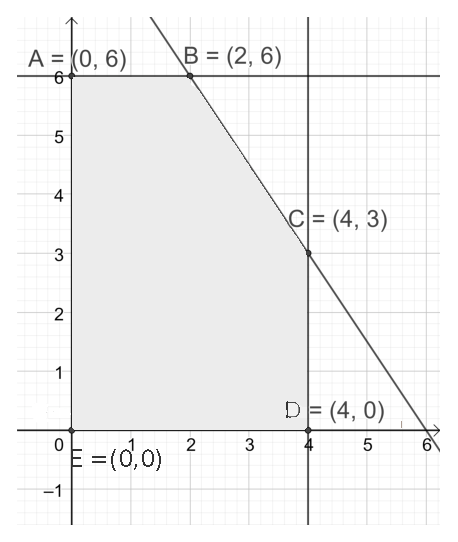
\includegraphics[width=180pt,height=180pt]{fig1.eps}
    \caption{Dopustiv region.}
    \label{fig:fig1}
\end{figure}
Pogledajmo sada niz (implicitnih) funkcija $3x_1 + 5 x_2 = c$, za $c \in \{3,20, 36\}$, kao na Slici~\ref{fig:fig2}. Jasno se vidi da prava $f = 36$ prolazi kroz tačku (vrh) regiona $(2,6)$, koja je svakako dopustiva. Takođe, vidimo da niti jedna druga funkcija $f=c, c > 36$ ne presijeca dopustiv region, odakle zaključujemo da je tačka $(2, 6)$ optimalno rješenje problema. Dakle, funkcija cilja ima maksimalnu vrijednost 36 i dostiže se u tački $(x_1, x_2)=(2,6)$.

Ovaj se postupak često naziva \emph{grafičkom metodom za linearno programiranje}. Ona se može koristiti za rješavanje bilo kojeg problema linearnog programiranja sa dvije promjenljive. Uz dodatni angažman,  ovu metodu je moguće   proširiti na problem sa tri promjenljive, što je krajnji domet grafičke metode. Za uopšten slučaj se koriste naprednije metode,  o kojima će biti riječi u narednim sekcijama.

\section{Standardna forma linearnog programiranja}

\begin{figure}[!ht]
    \centering
    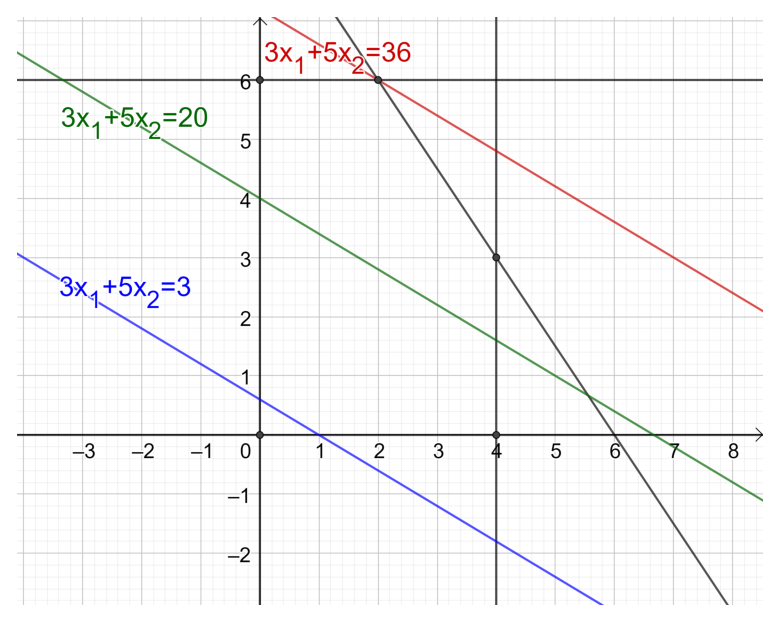
\includegraphics[width=180pt, height=180pt]{fig2.eps}
    \caption{Dodavanje $f = c$ i nalazak optimuma transliranjem po dopustivom regionu.}
    \label{fig:fig2}
 \end{figure}

 U ovoj sekciji govorimo o standardnoj formi modela linearnog programiranja. Uvedimo neke ključne pojmove koji se obično koriste u modelovanju i rješavanju problema linearnog programiranja. 

 Pođimo od pojmova \textit{resursi} i \textit{aktivnosti}. Pretpostavimo da u našem razmatranju imamo $m$ resursa i $n$ aktivnosti. Neki standardni resursi su vrijeme, novac, oprema, mašine, radnici itd. Aktivnosti uključuju ulaganje novca u određene projekte, dodjelu posla nekoj mašini ili radniku,  dostavljanje robe iz jednog u drugo mjesto, itd. 
  Najčešći tip primjene linearnog programiranja uključuje povezivanje resursa i aktivnosti, odnosno dodjelu resursa određenim aktivnostima. Dostupna količina svakog resursa je najčešće ograničena, pa aktivnosti trebaju biti pažljivo raspoređene u odnosu na odgovarajuće resurse.  Utvrđivanje ove raspodjele uključuje odabir vrsta i nivoa aktivnosti za koje se postiže najbolja moguća vrijednost  funkcije cilja. Funkcija cilja može da predstavlja mjeru dobiti (profita), mjeru vremena realizacije aktivnosti, mjeru broja proizvedenih proizvoda, itd.

 U nastavku navodimo notaciju koja se najčešće koriste u formiranju opšteg oblika modela linearnog programiranja (LP):

 \begin{itemize}
     \item $f$: funkcija cilja (dobiti) 
     \item $x_j$: količina aktivnosti $j$ ($j = 1,\ldots,n$);
     \item $c_j$: povećanje u profitu ako se količna aktivnosti $j$ poveća za jedan; %jediničnu vrijednost;
     \item $b_i$: ukupna količina resursa $i$ ($i=1,\ldots,m$) koja je dozvoljena za pridruživanje aktivnostima;
     \item $a_{ij}$: količina resursa $i$ koja se uzima za aktivnost $j$.
 \end{itemize}
 Prema ovoj notaciji, matematički model problema linearnog programiranja ima sljedeću postavku:
  
 \begin{align} 
       &\max  c_1 x_1 + \cdots + c_n x_n  \label{form:LP-1}\\
       & \mbox{t.d.} \nonumber \\
       & a_{i1}x_1 + a_{i2} x_{2} + \cdots + a_{in}x_n \leq b_i,\ i=1,\ldots,m \label{form:LP-2} \\
       %&\vdots \nonumber \\
       %& a_{m1}x_1 + a_{12} x_{m2} + \cdots + a_{mn}x_n \leq b_m \label{form:LP-3} \\
       & x_i \geq 0,\ i=1,\ldots,n.\label{form:LP-4}
 \end{align}

Postavka (\ref{form:LP-1})--(\ref{form:LP-4}) se još naziva i \emph{standardna forma} problema linearnog programiranja. Funkcija (\ref{form:LP-1}) se naziva funkcija cilja koju je potrebno maksimizovati pod uslovima (\ref{form:LP-2}), koji se nazivaju \emph{funkcionalna ograničenja}. Ograničenja (\ref{form:LP-4}) se nazivaju \emph{nenegativna ograničenja}. 

 Kompaktiniji oblik standardne forme LP-a je dat sa:
 \begin{align}
     & \max c^T x  \label{eq:LP-o1}\\
     & \mbox{t.d.} \nonumber \\
     &  A x \leq b \label{eq:LP-c1} \\
     & x \geq 0 \label{eq:LP-c2},
 \end{align}

 gdje je matrica $A \in \mathbb{R}^{m \times n}$, vektori  $x,c \in \mathbb{R}^n$ i vektor $b \in \mathbb{R}^{m}$.

 Treba imati na umu da se ograničenja (\ref{eq:LP-c1}) mogu zapisati i na sljedeći način:
 \begin{itemize}
     \item $Ax \geq b$;
     \item $Ax = b$;
     \item neke od promjenljivih $x_i\leqslant 0$.
 \end{itemize}
 Bilo koji problem koji koristi neke od prethodna tri ograničenja predstavlja i dalje problem linearnog programiranja. Dodavajući tzv. \emph{izravnavajuće promjenljive} (eng. slack variables) $s \in \mathbb{R}^m$ u linearni program sa ograničenjima $Ax \leq b$, dobijamo linearni program sa ograničenjima $Ax + s = b, s \geq 0$. Isto tako, linearni program sa ograničenja $Ax \geq b$ se može transformisati u ograničenja sa jednakostima dodavanjem izravnavajućih promjenljivih sa $Ax - s = b, s\geq 0$.

  Forma linearnog programa sa ograničenjima $Ax = b$ se naziva \emph{kanonska forma} linearnog programiranja. 
 
  Takođe, ako u linearnom
 programu postoji promjenljiva koja ne zadovoljava uslov nenegativnosti, ona se može zamijeniti razlikom dve nove nenegativne promenljive. Kanonski oblik linearnog programiranja je pogodan za efikasno izvođenje Gausovih transformacija  nad matricom problema, što se, na primjer, koristi u glavnim iteracijama simpleks metoda.   %, jer je svaki broj razlika dva nenegativna broja.

  U nastavku koristimo sljedeću terminologiju linearnog programiranja (LP):
 \begin{itemize}
     \item \emph{Rješenje} u standardnom matematičkom značenju najčešće označava rezultat izračunavanja, odnosno krajnje rješenje posmatranog problema. Međutim, u rješavanju problema LP-a to  nije slučaj. Bilo koja specifikacija vrijednosti promjenljivih  $(x_1,\ldots, x_n)$ se smatra rješenjem, bez obzira da li je riječ o željenom krajnjem rješenju ili čak o nekom rješenju koje i ne zadovoljava sva ograničenja. U zavisnosti od toga, rješenja  možemo podijeliti na:
     \begin{itemize}
         \item \emph{dopustiva rješenja} (eng. \emph{feasible solution}) -- podrazumijevaju ona rješenja koja zadovoljavaju sva ograničenja u modelu;
         \item \emph{nedopustiva rješenja} (eng. \emph{infreasible solution}) -- ona rješenja koja ne zadovoljavaju barem jedno od ograničenja u modelu. 
     \end{itemize}
   \item \emph{Dopustivi region}: označava skup svih rješenja koja su dopustiva. Ovo je prostor koji pretražujemo u svrhu pronalaska najboljeg rješenja modela. Takođe, može se desiti da problem nema niti jedno dopustivo rješenje. Za takav problem se kaže da je \emph{nedopustiv} (eng. infeasible). 
   \item \emph{Optimalno rješenje} je ono rješenje iz dopustivog regiona za koje je funkcija cilja najveća (pod pretpostavkom da maksimizujemo funkciju cilja), odnosno najmanja (pod pretpostavkom da minimizujemo funkciju cilja). Treba napomenuti da optimalno rješenje ne mora biti jedinstveno.  Npr. na Slici~\ref{fig:multi_solution} je prikazan dopustiv region sa ograničenjima $x_1, x_2 \geq 0, x_1 \leq 4 $ i $3 x_1 + 2 x_2 \leq 14$, dok je funkcija cilja, koja se maksimizuje, data sa $f = 3x_1 + 2 x_2$.  
  \end{itemize}
 
  \begin{figure}[!htb]
     \centering
     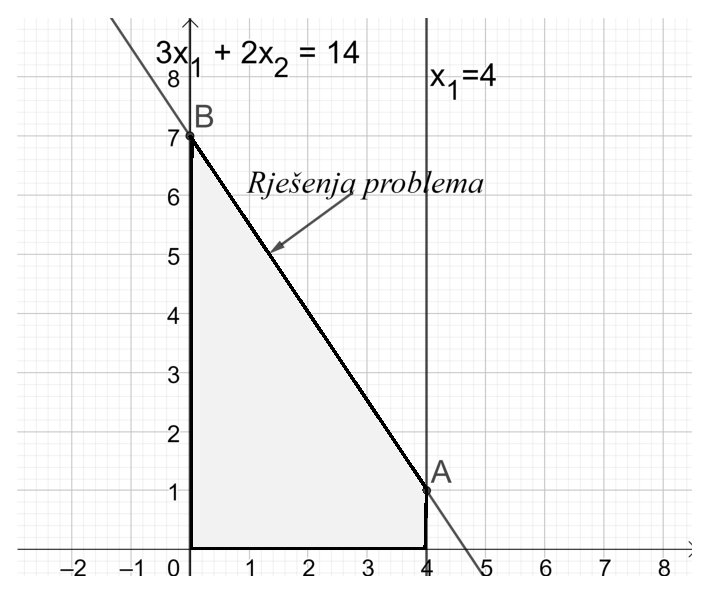
\includegraphics[width=160pt, height=160pt]{fig3.eps}
     \caption{LP sa više optimalnih rješenja.}
     \label{fig:multi_solution}
   \end{figure}
 
 Za razliku od nedopustivog problema, može se desiti i sasvim druga situacija, da je problem \emph{neograničen} (eng. unbounded). U tom slučaju vrijednosti neke od promjenljivih se mogu povećavati, da se ne naruši dopustivost, a tako da funkcija cilja (u problemu maksimizacije) teži ka beskonačno, tj. nije ograničena odozgo nekom vrijednošću. %Za takav problem kažemo da je \emph{neograničen}.
 
 Primjer neograničenog problema možemo vidjeti na Slici~\ref{fig:unbounded_solution}, gdje je potrebno maksimizovati funkciju $f = 3 x_1 + x_2$, pod uslovima $0\leq x_1 \leq 4$, te $x_2 \geq 0$. Kao što se može vidjeti,  kako vrijednost promjenljive $x_2$ teži ka beskonačnosti, tako i vrijednost funkcije $f$ teži ka beskonačnosti.
 
  \begin{figure}[H]
     \centering
     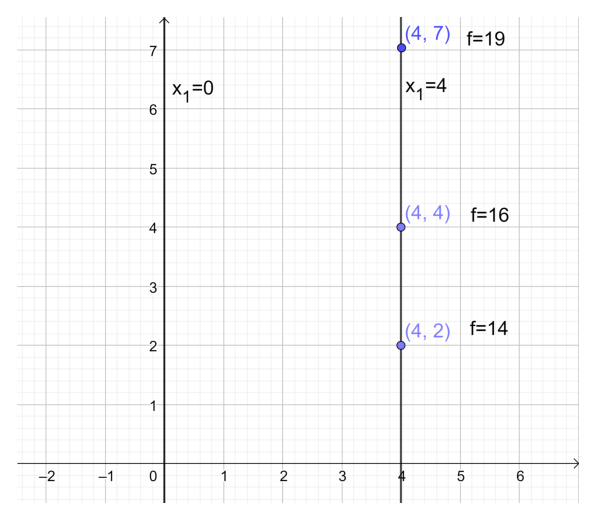
\includegraphics[width=180pt, height=180pt]{fig4.eps}
     \caption{Primjer LP-a koji je neograničen.}
     \label{fig:unbounded_solution}
 \end{figure}
 
 
%Uvedimo sada pojam \emph{ekstremnih tačaka}, koje igraju bitnu ulogu u simpleks metodi. Za rješenje $x$ kažemo da je \emph{ekstremna tačka} ako se nalazi u vrhu dopustivog regiona, odnosno u presjeku granica dopustivog regiona.

%Postoji važna povezanost između ovih tačaka i optimalnog rješenja LP-a, o čemu će biti riječi u nastavku ove knjige.
%Prije toga, za početak, razmotrimo bilo koji problem LP-a sa dopustivim rješenjima i ograničenim dopustivim regionom. Kao što će uskoro biti i pokazano, u tom slučaju ćemo da raspolažemo barem jednom tačkom vrh tog regiona i barem jednim optimalnim rješenjem. Nadalje, jedan od vrhova mora biti optimalno rješenje. Dakle, ako problem ima tačno jedno optimalno rješenje, to rješenje je tačka koja je vrh regiona. Ako problem ima više optimalnih rješenja, barem dva moraju biti rješenja koja su tačke  vrhova dopustivog regiona.

Treba imati na umu da (optimalno) rješenje LP-a ne mora da bude cjelobrojno. Budući da svaka promjenljiva odluke predstavlja nivo odgovarajuće aktivnosti, pretpostavlja se da se aktivnosti mogu izvoditi i na razlomljenim nivoima, odnosno, aktivnost  se ne dijeli samo na diskretne dijelove. 

Ako su domeni svih promjenljivih LP-a cjelobrojne vrijednosti, riječ je o modelu \emph{cjelobrojnog programiranja}. Ako pored cjelobrojnih, postoje i neke promjenljive koje uzimaju neprekidne vrijednosti, riječ je o modelima \emph{mješovitog--cjelobrojnog linearnog programiranja}. Veliki broj realnih problema koji dolaze iz prakse su upravo problemi mješovitog--cjelobrojnog linearnog programiranja.
 
%\section{Modelovanje nekih problema paradigmom linearnog programiranja}\label{sec:modeli_lp}


U naredna dva primjera opisani su modeli linearnog programiranja za dva poznata problema. 

\begin{primjer}
\emph{Problem optimalne dijete.} Pretpostavimo da su nam na raspolaganju namirnice $N_1, \ldots, N_n$. Jedinična cijena namirnice $N_j$ je $c_j>0, j = 1, \ldots, n$. U namirnicama su prisutni nutritivni elementi $e_i,i=1,\ldots,m$ pri čemu
namirnica $N_j$ sadrži $a_{ij} \geq 0$ nutritivnog elementa $e_i$, $i = 1, \ldots, n$, $j = 1, \ldots, m$. Svaka osoba u toku dana treba da unese barem $b_i$
jedinica nutritivnog elementa $e_i$. Potrebno je modelovati
sljedeći problem: 

Koliko je koje namirnice potrebno kupiti za (dnevnu) prehranu da bi se zadovoljila dnevna
potreba za svim nutritivnim elementima, a da se pri tome minimizuje cijena prehrane?
\end{primjer}
 
 \emph{Rješenje.}  Uvedimo realne promjenljive $x_j \geq 0$ za količinu hrane namirnice $N_j$, $j = 1, \ldots, n$, koja će se koristiti za prehranu. Funkcija cilja treba da odgovara minimizaciji cijene prehrane:
 $$f(x) = c_1 x_1 + \cdots + c_n x_n.$$
 
 Ograničenja problema su vezana za zahtjev da se zadovolji dnevna potreba za unosom svakog nutritivnog elementa. Odavde, slijedi da za $i$-ti element treba da bude zadovoljeno
 
 $$ a_{i,1} x_1 + \ldots + a_{i,n} x_n \geq b_i $$
 
 za svako $i=1,\ldots,m$. Dodajući još uslove nenegativnosti, $x_i \geq 0$, formulisali smo linearni model za ovaj problem.  
  \begin{primjer}
 \emph{Problem najboljeg pravca (problem linearne regresije)}. Zadani su podaci $(x_i, y_i), i = 1, \ldots , n$. Potrebno je odrediti pravu sa jednačinom $y = k x + l,
k, l \in \mathbb{R}$ koja, u smislu $l_1$ norme, najbolje aproksimira date podatke.  Napomenimo da umjesto $l_1$ često stoje i neke druge norme, poput euklidske, $l_2$ norme. Drugim riječima, potrebno je minimizovati  funkciju cilja $$f(k, l) = \sum_{i=1}^n |k x_i + l - y_i|.$$
 \end{primjer}

\emph{Rješenje}.
Označimo sa $z_i = |k x_i + l - y_i| = \max\{k x_i + l - y_i, y_i - k x_i - l \}$, $i=1,\ldots,n$. 


Primijetimo da apsolutna vrijednost ne odgovara direktno problemu LP-a, bilo da je prisutna u funkciji cilja ili ograničenjima, jer ona ne predstavlja linearnu funkciju (već je  linearna po dijelovima). Međutim, polazni problem možemo da preformulišemo na sljedeći  problem minimizacije linearnog programiranja: % ogranizenje |kx_i + l - y_i | <= z_i <=> dalje se svodi na dva ogranicenja...

$f(x) = c^T w = z_1 + z_2 + \ldots + z_n + 0\cdot k + 0 \cdot l$, pod uslovima
\begin{itemize}
    \item $ -z_i \leq k x_i + l - y_i$ 
    \item $ k x_i + l - y_i \leq z_i $, $i=1, \ldots, n$
    \item $k,l \in \mathbb{R}$. 
\end{itemize}
%% gdje je 
% $w_i = z_i, i=1,\ldots,n$, $w_{n+1} = k, w_{n+2} = l$, dok 
%  $c_i = 1, i=1,\ldots,n$, i $c_{n+1} = 0, c_{n+2} = 0$. 


 
Na kraju ove sekcije, navednimo nekoliko osnovnih implicitnih pretpostavki o problemima linearnog programiranja. 
\begin{enumerate} 
    \item \emph{Proporcionalnost.} Doprinos svake aktivnosti ciljnoj funkciji $f$ proporcionalan je njenom koeficijentu doprinosa, tj. $c_ix_i$. Doprinos svake aktivnosti svakom od  ograničenja u modelu proporcionalan je njenom  koeficijentu doprinosa, tj. $a_ix_i$.
    \item  \emph{Aditivnost.} Svaka funkcija u modelu je zbir  doprinosa pojedinih aktivnosti, npr. $f(x) = \sum_i a_i x_i$.
    \item \emph{Djeljivost}. Promjenljive odlučivanja se mogu podijeliti na vrijednosti koje nisu cijele, uzimajući u obzir  razlomljene vrijednosti, dok god su ograničenja zadovoljena.  

    \item \emph{Pouzdanost}. Pretpostavljamo da su vrijednosti parametara u modelu poznate
    sa velikom dozom pouzdanosti ili se barem tako tretiraju. Dobijeno optimalno rješenje je optimalno za razmatrani problem. Ako su vrijednosti parametara pogrešne, tada rezultujuće rješenje po pravilu ima malu (upotrebnu)  vrijednost.  
\end{enumerate}
%Ako model zadovoljava prethodne 4 pretpostavke, onda je riješ o modelu linearnog programiranja. 

\section{Teorija linearnog programiranja}
U ovom poglavlju ćemo formalno izvesti opšte uslove pod kojima se problem linearnog programiranja može riješiti. Prije nego što krenemo sa teoremama vezanim sa tim, kao i egzistenciju optimalnog rješenja u LP-u, navedimo nekoliko osnovnih definicija i pratećih teorema. 
 \begin{definition}
	Neka je $A \in \mathbb{R}^{m \times n}, b \in \mathbb{R}^m$. Skup $P=\{x \in \mathbb{R}^n \mid Ax \geq b\}$ se naziva poliedar u $\mathbb{R}^n$. 
\end{definition}


\begin{definition}
  Za skup $S \in \mathbb{R}^n$ kažemo da je konveksan akko za sve $x,y\in S$ i $\lambda\in [0, 1]$ vrijedi $\lambda x + (1 - \lambda)y \in S$
\end{definition}
\begin{definition}
   Za funkciju $f:\mathbb{R}^n \mapsto \mathbb{R}$ kažemo da je konveksna akko 
   $$ f( \lambda x + (1-\lambda) y) \leq \lambda f(x) + (1 -\lambda) f(y),$$
   za svaki $x,y \in \mathbb{R}^n$ i svaki $\lambda \in [0,1].$
\end{definition}
 Primijetimo da je svaka funkcija oblika $f(x_1, \ldots, x_n) = \sum_{i=1}^n c_i x_i = c^T x$ za neke $c_i \in \mathbb{R}$, konveksna, što se lako provjerava na osnovu definicije konveksnosti. Dakle, LP u svom opštem obliku  ima ciljnu funkciju koja je konveksna. Geometrijska interpretacija konveksnosti funkcije je prikazana na Slici~\ref{fig:convex_function}.

%\begin{figure}
%    \centering
%    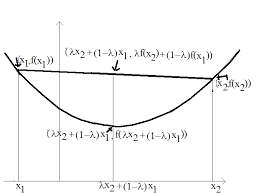
\includegraphics[width=180pt,height=180pt]{convex_function.png}
%    \caption{Primjer konveksne funkcije}
%    \label{fig:convex_function}
%\end{figure}
\begin{figure}
   \centering
\begin{tikzpicture}
\begin{axis}[width=5in,axis equal image,
    axis lines=middle,
    xmin=0,xmax=8,
    xlabel=$x$,ylabel=$y$,
    ymin=-0.25,ymax=4,
    xtick={\empty},ytick={\empty}, axis on top
]

% 
\addplot[thick,domain=0.25:7,blue,name path = A]  {-x/3 + 2.75} coordinate[pos=0.4] (m) ;
\draw[thick,blue, name path =B] (0.15,4) .. controls (1,1) and (4,0) .. (6,2) node[pos=0.95, color=black, right]  {$f(x)$} coordinate[pos=0.075] (a1)  coordinate[pos=0.95] (a2);
\path [name intersections={of=A and B, by={a,b}}];

% 
\draw[densely dashed] (0,0) -| node[pos=0.5, color=black, label=below:$a$] {}(a1);
\draw[densely dashed] (0,0) -| node[pos=0.5, color=black, label=below:$x_{1}$] {}(a);
\draw[densely dashed, name path=D] (3,0) -|node[pos=0.5, color=black, label=below:$\lambda x_{1}+ (1-\lambda)x_{2}$] {} node[pos=1, fill,circle,inner sep=1pt] {}(m);
\draw[densely dashed] (0,0) -|node[pos=0.5, color=black, label=below:$x_{2}$] {}(b);
\draw[densely dashed] (0,0) -|node[pos=0.5, color=black, label=below:$b$] {}(a2);

% 
\path [name intersections={of=B and D, by={c}}] node[fill,circle,inner sep=1pt] at (c) {}; 

% 
\node[anchor=south west, text=black] (d) at (0.75,3) {$f[\lambda x_{1}+(1-\lambda)x_{2}]$};
\node[anchor=south west, text=black] (e) at (5,2.5) {$\lambda f(x_{1})+(1-\lambda)f(x_{2})$};
\draw[-{Latex[width=4pt,length=6pt]}, densely dashed] (d) -- (c);
\draw[-{Latex[width=4pt,length=6pt]}, densely dashed] (e) -- (m);
\end{axis}
\end{tikzpicture}
   \caption{Konveksna funkcija: geometrijska interpretacija.}
   \label{fig:convex_function}
\end{figure}

\begin{definition}
   Neka su dati vektori $z^{(i)} \in \mathbb{R}^n$,  te $\lambda_i \in [0,1]$ $i=1,\ldots,m$ tako da je $\sum_{i=1}^m \lambda_i = 1.$ Vektor $x =  \sum_{i=1}^m \lambda_i z^{(i)}$ se naziva konveksna kombinacija vektora $z^{(i)}, i=1,\ldots, n$. 
\end{definition}

Konveksne funkcije imaju lijepa svojstva sa stanovišta teorije i u kombinaciji sa konveksnim skupovima čine osnov  teorije optimalnosti. Inače, vrijedi sljedeća teorema.
\begin{thm}\label{thm:globalopt}
  Neka je $f : S \mapsto \mathbb{R}$ konveksna funkcija definisana na konveksnom skupu $S \subseteq \mathbb{R}^n$. Ako funkcija $f$ u tački $x^* \in S$
 postiže lokalni minimum, onda ta tačka predstavlja i tačku globalnog minimuma.
\end{thm}

\begin{comment}
	
\begin{proof}  
 Neka je $x^* \in S$ tačka lokalnog minimuma funkcije $f$. Prema tome, postoji $r >0$ za što vrijedi $f(x^*) \leq f(x)$, za sve $x \in S \cap K(x^*, r)$. Odaberimo vektor $x \neq x^* \in S$ i definišimo vektor 
 $z(\lambda) = \lambda x + (1 - \lambda) x^*$ za neki $\lambda \in [0, 1]$. Kako je $S$ konveksan, slijedi da je $z \in S$.  Definišimo $\lambda_0 <  \min\{1, r ||x - x^*||^{-1}\}$, $\lambda_0 \in (0, 1]$. Tada za svaki $\lambda \in (0, \lambda_0)$ vrijedi 
 \begin{equation}
     ||z(\lambda) - x^* ||  =  || \lambda ( x - x^*) ||  = \lambda ||x - x^* || \leq \lambda_0 ||x - x^* ||  \leq r.
 \end{equation} 
 Dakle, pokazano je da je $z(\lambda) \in S \cap K(x^*, r)$. Prema tome, vrijedi 
 \begin{equation} 
     f(x^*) \leq f(z(\lambda)) = \lambda f(x) + (1-\lambda) f(x^*) 
 \end{equation} 
 odakle slijedi 
 \begin{equation} 
      \lambda f(x^*) \leq   \lambda f(x) \Rightarrow f(x^*) \leq f(x),  
 \end{equation}
 za proizvoljno odabrano $x \in S$, čime smo pokazali teoremu. 
\end{proof} 
% http://home.ku.edu.tr/~mturkay/indr262/Indr262LectureNotes_2-LPModels.pdf
% (Assumptions of Linear Programming)
\\ 
U sljedeće dvije definicije definišimo pojmove poliedra, hiperravni i poluprostora. 

\end{comment} 

 \begin{definition}
   Neka je $a\in \mathbb{R}^n $ i $b \in \mathbb{R}$. Skup $\{ x \in \mathbb{R}^n \mid a^T x = b \}$ se naziva hiperravan u $\mathbb{R}^n$ čiji je vektor normale $a$, dok se $\{ x \in \mathbb{R}^n \mid a^T x \geq b \}$ naziva poluprostor.  
\end{definition}


 Pokažimo sada da je poliedar svakog LP-a konveksan skup. To je važna karakteristika, jer se uslovima problema LP-a formira upravo poliedar kao skup dopustivih rješenja.


 \begin{prop} Vrijede sljedeće tvrdnje: \\
  ($i$)  Poluprostor u $\mathbb{R}^n$ je konveksan skup.  \\
  ($ii$) Presjek konačno mnogo konveksnih skupova je konveksan skup. 
\end{prop}

 \begin{proof}
  ($i$) Neka je dat poluprostor $P = \{ x \in \mathbb{R}^n \mid a^T x \geq b \}$. Uzmimo $x, y \in P$, te neko $\lambda \in [0, 1]$. Treba da pokažemo da konveksna kombinacija ova dva vektora   pripada $P$. Iz $x \in P$, slijedi  $a^T x \geq b$. Takođe, kako je $y \in P$, onda  je  $a^T y \geq b$. 
  Sada  imamo sljedeće:
   \begin{align}
      a^T (\lambda x) \geq \lambda b \\
      a^T ((1-\lambda) y) \geq (1-\lambda) b 
   \end{align}
  Sabirajući posljednje dvije nejednakosti, dobijamo 
  \begin{equation}
      a^T( \lambda x + (1 - \lambda) y ) \geq b,
  \end{equation}
  odakle slijedi da $\lambda x + (1-\lambda) y \in P$, čime je tvrdnja dokazana.
  
  ($ii$) Neka su $S_1,\ldots, S_n$ konveksni skupovi. Ako $x,y \in \cap_{i=1}^n S_i$, onda slijedi da $x,y \in S_i$ za svaki $i=1,\ldots,n$. Zbog konveksnosti svakog od skupova,  
  $\lambda x + (1 - \lambda) y \in S_i$, za svaki $i=1,\ldots,n$. Prema tome, vrijedi $ \lambda x + (1-\lambda) y \in \cap_{i=1}^n S_i$, odakle slijedi da je $\cap_{i=1}^n S_i$ konveksan. 
\end{proof}

 Iz prethodne propozicije vrijedi sljedeća posljedica.

 \begin{poslje}
    Poliedar $P$ nekog problema LP-a je konveksan skup.	
 \end{poslje}
 
 \begin{proof}
   Definišimo $S_i:= \{(x_1,\ldots, x_n) \in \mathbb{R}^n \mid C_i^T x \geq b_i \}$, gdje je  $C_i = (a_{i,1}, \ldots, a_{i, n}),$  $ i=1,\ldots, m$. Kako je $\cap_{i=1}^m S_i$ poliedar koji odgovara problemu LP-a, na osnovu prethodne propozicije ($ii$), slijedi tvrdnja. 
 \end{proof}

 Kako je poliedar konveksan skup, Teorema~\ref{thm:globalopt} nam garantuje da, uz pretpostavku da postoji lokalni minimum (maksimum), onda postoji  i globalni minimum (maksimum), odnosno optimalno rješenje zadanog problema LP-a. 
 
  Nadalje, formalno definišimo pojmove ekstremne tačke (eng. extreme point), vrha (eng. vertex) i baznog dopustivog rješenja koji igraju bitnu ulogu u teoriji linearnog programiranja. 


\begin{definition}
   Neka je $P$ poliedar u $\mathbb{R}^n$.  Vektor $x \in P$ se naziva ekstremna tačka poliedra $P$
   ako ne postoje vektori $y, z \in P$, $y \neq x, z \neq x$ i skalar $\lambda \in [0, 1]$ takvi da je  $x = \lambda y + (1-\lambda)z$.
\end{definition}

Dakle, ekstremna tačka poliedra se ne može napisati kao netrivijalna konveksna kombinacija tačaka iz tog poliedra. 
 
  Neformalno rečeno, ako je  $x$ ekstremna tačka poliedra, tada ona ne leži između neke dvije tačke $y$ i $z$   poliedra $P$.
 
 
\begin{definition}\label{def:vrhPoliedra}
   Neka je dat poliedar $P \subseteq \mathbb{R}^n$. Tačku $x \in P$ nazivamo vrh (poliedra) ako postoji linearna funkcija  $c^T x$ koja je strogo minimizovana u toj tački, tj. za sve  $y\in P, y \neq x$, vrijedi $c^T x < c^T y$. 
\end{definition}
Geometrijski posmatrano,  vrh poliedra $P$ je ona tačka poliedra  kroz koju možemo provući poluravan (hiperravan) sa svojstvom da se sve tačke iz $P$ (izuzev vrha) nalaze sa iste strane te poluravni.

Uvedimo sada nekoliko novih pojmova koji će nam pomoći da definišemo bazno dopustivo rješenje.

\begin{definition}\label{dfn:lp_aktivan}
   Neka je poliedar $P$ zadan na sljedeći način
   \begin{itemize}
       \item $a_i^T x \geq b_i, i \in C_1$
       \item $a_i^T x = b_i, i \in C_2 $
       \item $a_i^T x \leq b_i, i \in C_3 $. 
   \end{itemize}
   Ako za neko $x^* \in P$ i neki $i_0 \in C_1 \cup C_1 \cup C_2$ vrijedi 
   $a_{i_0}^T x^* = b_{i_0}$, onda je indeks (ograničenje) $i_0$ aktivan u $x^*$. 
\end{definition}

\begin{definition}
      Neka je zadan poliedar iz Definicije~\ref{dfn:lp_aktivan}. Neka je 
      $I = \{ i \in C_1 \cup C_2 \cup C_3 \mid a_i^T x^* = b_i \}$  skup indeksa aktivnih u $x^*\in \mathbb{R}^n$.  Ako je skup $\{ a_i \mid i \in I \}$ linearno nezavisan, onda se $x^*$  naziva bazno rješenje. 
\end{definition}
% https://faculty.math.illinois.edu/~mlavrov/docs/482-fall-2019/lecture8.pdf
\begin{definition}
	 Bazno dopustivo rješenje $x^*$ je bazno rješenje koje zadovoljava  uslove linearnog programa. 
\end{definition}
Pokažimo sada da  vrhovi, ekstremne tačke poliedra i bazna dopustiva rješenja predstavljaju ekvivalentne pojmove kada je riječ o linearnom programiranju.

\begin{thm}
   Neka je $P$ poliedar i neka je $x^* \in P$. Sljedeće tri tvrdnje su ekvivalentne:
   \begin{enumerate}
       \item $x^*$ je vrh poliedra;
       \item $x^*$ je ekstremna tačka poliedra;
       \item $x^*$ je bazno dopustivo rješenje (BDR).
   \end{enumerate}
\end{thm}

\begin{proof}
      Pokažimo da vrijedi $1 \Rightarrow 2, 2 \Rightarrow 3$, pa onda $3 \Rightarrow 1$, čime ćemo pokazati ekvivalenciju sve tri tvrdnje.
      
      $1 \Rightarrow 2$. Neka je $x^*$ vrh poliedra. Iz Definicije~\ref{def:vrhPoliedra} slijedi da 
      postoji $c\in \mathbb{R}^n$ tako da $c^Tx^* < c^T x$, za sve $x \in P, x \neq x^*$. Pretpostavimo da $x^*$ nije ekstremna tačka poliedra $P$. 
      To bi značilo da postoje $y,z \in P$, koji su različiti od $x^*$, takvi da se $x^*$ može predstaviti kao njihova (netrivijalna) konveksna kombinacija, tj. $x^* = \lambda y + (1 - \lambda) z $, za neko $\lambda \in (0,1 )$. Na osnovu pretpostavke je $c^T x^* < c^T y$.  Sada je 
      \begin{align}
          &c^T x^* = c^T ( \lambda y + (1 - \lambda) z )  = c^T( \lambda y) + c^T((1- \lambda) z) > \nonumber \\
          &>\lambda c^T x^* + ( 1 - \lambda) c^T x^* = c^T x^*.
      \end{align}
      što je nemoguće, odakle slijedi tvrdnja. 
      
      $2 \Rightarrow 3$.
       Ovu implikaciju ćemo dokazati kontrapozicijom. Pretpostavimo da tačka $x^*$ nije BDR i pokažimo da iz toga slijedi da ona nije ni ekstremna tačka.
      Bez smanjenja opštosti, zapišimo poliedar $P$ na sljedeći način.
       \begin{align}
            & a_i^T x \geq b_i, i \in C_1 \\
            & a_i^T x  = b_i, i \in C_2.
       \end{align}
       Ako $x^*$ nije BDR, to znači da je broj uslova koji su aktivni u $x^*$ manji od $n$. 
       Ako sa $I \subseteq C_1 \cup C_2$ označimo skup aktivnih indeksa u $x^*$, onda 
       je $\{ a_i \mid i \in I \} \subseteq \mathbb{R}^n$ pravi potprostor od $\mathbb{R}^n$.  Prema tome, postoji vektor $d \in \mathbb{R}^n \setminus \{0\}$ za koji vrijedi $a_i^T d = 0$, za sve $i \in I$. Definišimo vektore 
       $$ y = x^* + \epsilon d, z = x^* - \epsilon d, $$
       za neko $\epsilon > 0$, pa pokažimo da $y, z \in P$.
       
       Ako je $i \in I$, onda je $$a_i^T y = a_i^T (x^* + \epsilon d) = a_i^T x^* + \epsilon a_i^T d = a_i^T x^* = b_i. $$ Preostalo je da pokažimo da za $i \not \in I$ vrijedi $a_i^T y \geq b_i$, odakle bi slijedilo da $y \in P$. 
       
       Dakle, $a_i^T y = a_i^T (x^* + \epsilon d) = a_i^T x^* + \epsilon a_i^T d $. Ako je $a_i^T d \geq 0$, slijedi da je 
       $a_i^T y > a_i^Tx^* \geq b_i$, odakle slijedi da   $y \in  P$. Ako je $a_i^T d < 0$, onda odaberimo takve $\epsilon$ za koje će vrijediti $a_i^T x^* + \epsilon a_i^T d > b_i$. Interval   vrijednosti za $\epsilon$ dobijemo iz sljedećeg računa:
       $$ a_i^T x^* + \epsilon a_i^T d > b_i \Rightarrow \epsilon < \frac{b_i - a_i^T x^*}{a_i^T d}  $$
       Za svaki $\epsilon \in \left(0,  \frac{b_i - a_i^T x^*}{a_i^T d} \right)$ vrijedi $a_i^T y > b_i$, odakle slijedi $y \in P$. Slično pokažemo i da vrijedi $z \in P$. 
       Prema tome, lako je vidjeti da vrijedi $x^* = \frac{1}{2}y +\frac{1}{2} z$. Dakle, $x^*$ se dobija kao netrivijalna konveksna kombinacija, što je u suprotnosti sa definicijom ekstremne tačke. 
       
       $3 \Rightarrow 1$. Neka je $x^*$ BDR. Treba da pokažemo da je  $x^*$  takođe vrh poliedra $P$. Označimo sa $I$ skup aktivnih indeksa u $x^*$ i definišimo $c = \sum_{i \in I} a_i$.  Tada imamo 
       $ c^T x^* = \sum_{i \in I } a_i^T x^* = \sum_{i \in I} b_i$. Za proizvoljno $x \in P$ dobijamo
       \begin{equation}\label{eq:3_impl_1}
          c^T x = \sum_{i \in I} a_i^T x \geq c^T x^*  
       \end{equation}
     Iz toga vidimo da je $x^*$ rješenje LP problema minimizacije. Jednakost u (\ref{eq:3_impl_1}) vrijedi ako i samo ako je $a_i^T x = b_i$ za sve $i \in I$. Kako je $x^*$ BDR, broj linearno nezavisnih vektora $a_i, i \in I$ koji su  aktivni u $x^*$ je jednak $n$, pa sistem $a_i^T x = b_i, i \in I$ ima jedinstveno rješenje koje je upravo $x^*$. Prema tome, pokazano je da postoji vektor $c \in \mathbb{R}^n$ za koji vrijedi $c^T x > c^T x^*$ za sve $x \neq x^*$, $x \in P$, odake, na osnovu definicije vrha poliedra, slijedi tvrdnja. 
\end{proof} 
U nastavku ćemo dati potrebne uslove za postojanje BDR-a, tj. 
 ekstremne tačke poliedra. Takođe, daćemo i postupak za konstrukciju BDR-a, te ćemo uvesti pojam degenerativnog rješenja.

\begin{thm}
   Neka je $P = \{ x \in \mathbb{R}^n \mid A x = b, x \geq 0\}, A \in \mathbb{R}^{m \times n}, b \in \mathbb{R}^m$ i $rang(A)= m, m < n$.
   Vektor $x$ je bazno rješenje  akko je $A x = b$ i ako postoje indeksi $p_1,p_2,\ldots, p_m$ takvi da vrijedi:
   \begin{enumerate}
       \item kolone $A_{p_1},\ldots, A_{p_m}$ su linearno nezavisne
       \item ako $i \notin \{p_1,\ldots, p_m\}$, onda $x_i = 0$.
   \end{enumerate}
   
\end{thm}
Iz prethodne teoreme možemo zaključiti sljedeće.  Da bismo  konstruisali bazno rješenje, potrebno je izvršiti sljedeće korake:
\begin{enumerate}
    \item Odaberemo $m$ linearno nezavisnih kolona $A_{p_1}, \ldots, A_{p_m}$ matrice $A$.
    %\item Postavimo $x_i = 0$, za sve $i \in \{p_1,\ldots, p_m \}$.
    \item Riješimo sistem $B x_B = b$, za $x_B = [x_{p_1}, \ldots, x_{p_m}]$ i $B= [A_{p_1}. \ldots, A_{p_m}]$
    \item Dodijelimo $$x = (x_1,\ldots, x_n):= \begin{cases}
    	          0, j  \not   \in \{ p_i \mid i=1,\ldots, m\} \\
    	          (x_B)_i, j \in \{ p_i \mid i=1,\ldots, m\}
    \end{cases},$$  čime dobijamo bazno rješenje. 

\end{enumerate} 
 
Promjenljive $x_{p_1},\ldots, x_{p_m}$ se nazivaju \emph{bazne promjenljive}, dok vektore $A_{p_1}, \ldots, A_{p_m}$ nazivamo \emph{baznim vektorima}. Indekse $p_1,\ldots, p_m$ nazivamo \emph{bazni indeksi}, a matricu $B$ matricom baze. 


Definišimo sada pojam \emph{degenerativnog} rješenja i degenerativnog baznog rješenja. 

\begin{definition}
      Neka je dat poliedar $P = \{ x \in \mathbb{R}^n \mid a_i^T x \geq b_i, x_i \geq 0, i=1,\ldots,m \}$. Za bazno rješenje $x^*\in \mathbb{R}^n$ kažemo da je degenerativno ako je više od $n$  ograničenja aktivno u $x^*$. 
      
\end{definition}

\begin{definition}
      Neka je $P = \{ x \in \mathbb{R}^n \mid A x = b,  x_i \geq 0, i=1,\ldots,m \}, A \in \mathbb{R}^{m \times n}, b \in \mathbb{R}^m$    i neka je $x$ bazno rješenje. Vektor $x$ nazivamo degenerativno bazno rješenje ako je više od $n-m$ komponenti u vektoru $x$   jednako 0.
\end{definition}
U sljedećem primjeru ćemo pokazati kako se pronalazi bazno rješenje, te kako izgleda degenerativno bazno rješenje.

\begin{primjer} Zadajmo poliedar $P= \{ (x_1,x_2,x_3)^T \mid x_2 - x_1 = 0, x_1 + x_2 +   x_3 = 2, x_1,x_2,x_3 \geq 0 \}$.  Pronaći bazna dopustiva rješenja i odrediti jesu li ona degenerativna. 
\end{primjer}

\emph{Rješenje.} Lako je vidjeti da je  
$A=\left (\begin{array}{ccc}
   -1  &  1 & 0  \\
   1  &  1 & 1 \\
\end{array} \right )$ te $b = [0\ 2]^T$. Prateći postupak konstrukcije baznog rješenja, pronađimo dvije linearno nezavisne kolone matrice $A$. Npr. možemo uzeti prve dvije kolone, pa je matrica $B=\left (\begin{array}{cc}
   -1  & 1    \\
   1  &  1   \\
\end{array} \right ) .$ Riješimo sistem jednačina (stavka 2), odakle je rješenje $x_B = [1\ 1]^T$, a krajnje rješenje je $x^* = [1\ 1\ 0]^T$. Kako je 
$x^*$ aktivan u sva tri uslova $x_2 - x_1 = 0, x_1 + x_2 +  x_3 = 2$ i $x_3 = 0$, rješenje je nedegenerativno bazno dopustivo rješenje.  Takođe, možemo odabrati drugu i treću kolonu matrice za bazne kolone (kao i prvu i treću), odakle bismo dobili rješenje $x^* = [0\ 0\ 2]^T$, aktivno u četiri uslova, pa smo dobili degenerativno bazno dopustivo rješenje. 


U nastavku govorimo o egzistenciji optimalnog rješenja problema LP-a. Definišimo prvo pojam pravca u poliedru.

 \begin{definition}
       Poliedar $P$ sadrži pravac akko postoji $x \in P$ i $d \in \mathbb{R}^n \setminus \{0\}$ tako da je $x + \lambda d \in P$, za sve $\lambda \in \mathbb{R}$. 
 \end{definition}
Primjer pravca koji postoji u poliedru je dat na Slici~\ref{fig:extreme-ray}. 
  \begin{figure}[!htb]
	\centering
	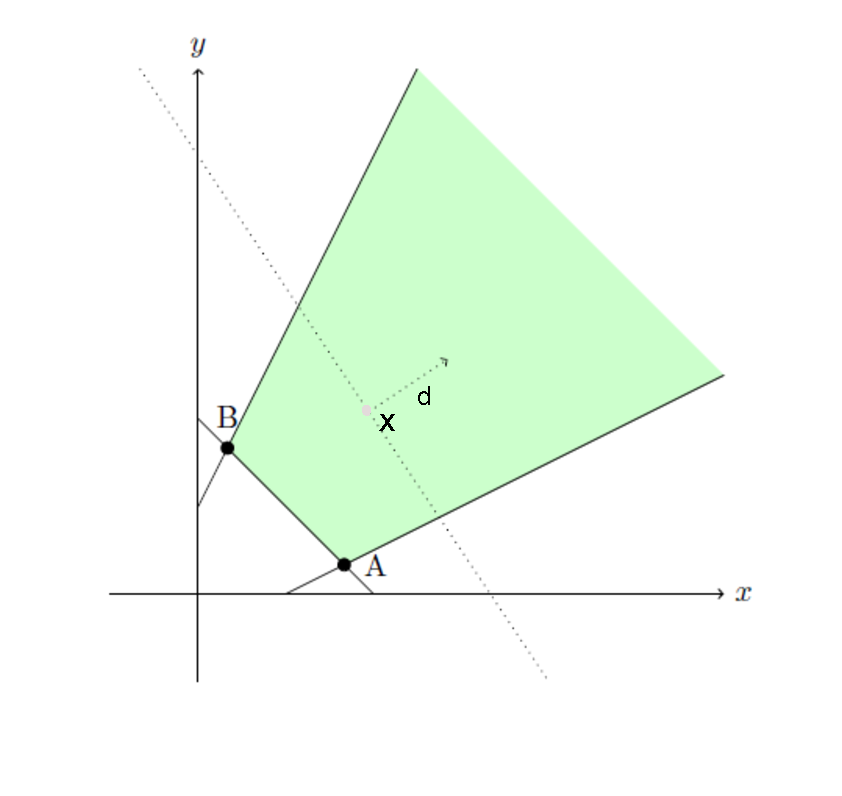
\includegraphics[width=200pt,height=200pt]{extremerays.eps}
	\caption{Pravac u poliedru}
		\label{fig:extreme-ray}
   \end{figure}  

Sljedeću teoremu, koja daje vezu između ekstremnih tačaka poliedra i dopustivih pravaca, navodimo bez dokaza.

\begin{thm}\label{thm:pravac}
   Neka je dat poliedar $P=\{ x \in \mathbb{R}^n  \mid a_i^T x \geq b_i, i=1,\ldots,m\} \neq \emptyset$. Tada su sljedeće tri tvrdnje ekvivalentne:
   \begin{itemize}
       \item  Poliedar $P$ ima barem jednu ekstremnu tačku.
       \item Poliedar $P$ ne sadrži pravac.
       \item Postoji $n$ linearno nezavisnih vektora  među kolonama matrice $A$. %, tj. među $a_i, i=1,\ldots,m$.
   \end{itemize}
\end{thm}

Sljedeća teorema nam daje dovoljan uslov za postojanje optimalnog rješenja koje je uvijek jedna od ekstremnih tačka poliedra (dopustivog regiona) problema linearnog programiranja.

\begin{thm}
   Neka je zadan problem LP-a sa funkcijom cilja $c^Tx$ koju je potrebno minimizovati na poliedru $P$. Pretpostavimo da za poliedar $P$ postoji barem jedna ekstremna tačka i da za dati problem postoji optimalno rješenje. Tada postoji i optimalno rješenje koje je ekstremna tačka poliedra $P$.
\end{thm}

\begin{proof}
         Sa $O^* \not = \emptyset$ označimo skup svih optimalnih rješenja  nad poliedrom $P= \{ x \in \mathbb{R}^n \mid A x \geq b \}$, te neka je $c^T x^* = v$, za sve $x^* \in O^*$. Vidimo da je 
         $O^* = \{ x \in \mathbb{R}^n \mid A x \geq b, c^T x = v  \}$ takođe poliedar i da važi $O^* \subset P$. Iz Teoreme~\ref{thm:pravac} slijedi da poliedar $P$ ne sadrži pravac. Iz toga zaključujemo da ni $O^*$ nema pravac, odakle slijedi da $O^*$ ima barem jednu ekstremnu tačku (stavka 1 Teoreme~\ref{thm:pravac}). Označimo tu ekstremnu tačku sa $q^*$. Pokažimo da je to ujedno i ekstremna tačka od $P$.  Ako bismo pretpostavili da $q^*$ nije ekstremna tačka poliedra $P$, po definiciji, slijedi da postoje $y, z \in P$ tako da $q^* = \lambda y + ( 1 - \lambda ) z $, $y \neq q^*, z \neq q^*, \lambda \in [0, 1]$. Kako je $q^* \in O^*$, slijedi 
         $$ v = c^T q^* = c^T (  \lambda y + ( 1 - \lambda ) z ) = \lambda 
        \underbrace{ c^T y}_{ \geq v} + ( 1 - \lambda ) \underbrace{c^T z}_{\geq v} \geq \lambda v + (1 - \lambda) v = v,$$
        odakle imamo $c^T y = v$ i $c^T z = v$, dakle $y, z \in O^*$. Prema tome, $q^*$ nije ekstremna tačka od $O^*$. Dolazimo do kontradikcije, odakle zaključujemo da $q^*$ mora biti  ekstremna tačka i od  $P$.
\end{proof}
 

 Navedimo sada i važnu posljedicu prethodne teoreme.
 \begin{poslje}
Ako  rješavamo problem minimizacije LP-a na poliedru $P$ koji ima barem jednu ekstremnu tačku, tada vrijedi tačno jedna od sljedeće dvije tvrdnje:
   \begin{enumerate}
       \item Funkcija cilja ima vrijednost $- \infty$ (funkcija cilja je neograničena).
       \item Postoji ekstremna tačka u kojoj funkcija cilja dostiže optimalno rješenje. 
   \end{enumerate}
 \end{poslje}

 Prethodna tvrđenja nam daju bazu za konstrukciju simpleks metoda koji je, kao što smo već pomenuli, jedna od najpoznatijih i najefikasnijih generalnih metoda za rješavanje LP problema.
Kako ćemo vidjeti u narednom poglavlju, simpleks metoda je zasnovana na iterativnom posjećivanju vrhova poliedra  u cilju pronalaska optimalnog rješenja.

\section{Neke tehnike u modelovanju problema linearnog programiranja}

\emph{Apsolutna vrijednost u funkciji cilja}.   Pretpostavimo da imamo model zadat sa 
\begin{align}
	&\min \sum_{j \in J}   |x_j| \nonumber \\
	& \mbox{t.d.} \nonumber \\
	& \sum_{j\in J} a_{ij} x_j \leq b_i, \forall i\in I  \nonumber \\
	& x_j \in \mathbb{R}, \forall j \in J. \label{eq:lp_abs}
\end{align} 
 
Kao što znamo, apsolutna vrijednost nije linearna funkcija, ali se ovaj model može transformisati u model linearnog programiranja na sljedeći način: 
svaku   promjenljivu ćemo zapisati kao razliku dvije pozitivne promjenljive, tj.  $x_j = x_j^+ - x_j^-$, a apsolutnu vrijednost kao zbir dvije pozitivne promjenljive, tj. $|x_j|= x_j^+ + x_j^-$. Prema tome, prethodni model se transformiše  u ekvivalentan (u smislu optimalnog rješenja) model  
\begin{align}
	&\min \sum_{j \in J}  (x_i^+ + x_i^-) \nonumber \\
	& \mbox{t.d.} \nonumber \\
	&\sum_{j\in J} a_{ij} (  x_i^+ - x_i^- ) \leq b_i, \forall i \in I \nonumber \\
	&  x_i^+, x_i^- \geq 0, \forall j\in J. \label{eq:lp_abs_transformed}
\end{align}
 
 Može se pokazati da za optimalno rješenje prethodnog modela vrijedi  $x^{+}\cdot x^{-}= 0$.  
   Pretpostavimo da je $x_j^*$, $j \in J$ optimalno rješenje LP-a (\ref{eq:lp_abs}). Rješenje za LP  (\ref{eq:lp_abs_transformed})  dato u obliku 
  $(x_j^+)^* = x_j^*$  ako je $x_j^* \geq 0$, a inače $(x_j^+)^* = 0$ i slično $(x_j^-)^* = - x_j^*$  ako je $x_j^* \leq 0$, a inače $(x_j^-)^* = 0$ je dopustivo za (\ref{eq:lp_abs_transformed}). Lako se provjeri da su vrijednosti ova dva rješenja u odnosu na odgovarajuće funkcije cilja jednake. Pokažimo da je rješenje  $((x^+)^*, (x^-)^*)$ ujedno i optimalno rješenje modela (\ref{eq:lp_abs_transformed}).   Neka je rješenje $(x^+, x^-)$ optimalano za model  (\ref{eq:lp_abs_transformed}) za koje postoji neko $j$ tako da  $x^{+}_j, x^{-}_j > 0$. Bez smanjenja opštosti, pretpostavimo da je $x^{+}_j \geq x^{-}_j$. 
  Rješenje $(y^+, y^-)$  za koje je $y^+_i = x^+_i$ i $(y^-_i = x^-_i)$ za sve $i \neq j$
   i $y^+_j = x^{+}_j - x^{-}_j \geq 0$ i $(y^-_j)^*=0$ je dopustivo, i daće istu ili manju vrijednost funkcije cilja nego rješenje prije transformacije. Prema tome, ukoliko postoje, optimalna rješenja LP-a (\ref{eq:lp_abs_transformed}) su među onim rješenjima za koje vrijedi da  barem jedna od promjenljivih $x_j^+$ ili $x_j^-$, $j \in J$  jednaka 0. Sva ostala rješenja su podoptimalna za model (3.15) i sigurno mogu da budu izuzeta iz domena rješenja (\ref{eq:lp_abs_transformed}) bez gubitka optimalnosti.   Prema tome, za svako dopustivo rješenja $x$ za (\ref{eq:lp_abs}) postoji dopustivo rješenje  $(x^+, x^-)$ za (\ref{eq:lp_abs_transformed}) i obrnuto. Pri tome, vrijednosti funkcija cilja ovakvih rješenja su jednake. Prema tome, ova dva modela su ekvivalenta. Može se pokazati da transformacija vrijedi i opštiji slučaj, tj. kada je funkcija cilja data sa $f(x)= \sum_{j \in J} c_j |x_j|, c_j \geq 0, j \in J$.


\emph{Min-max problem}. Neka je dat sljedeći model: 
\begin{align*}
	 &\min_{x} \max_{k \in K} \sum_{j \in J} c_{kj} x_j \\
	 &{\mbox{t.d.}} \nonumber \\
	 & \sum_{j \in J} a_{ij} x_j \leq b_i\  \forall i \in I \\
	 & x_j \geq 0\ \forall j \in J.
 \end{align*}
 Ovaj  model se transformiše u model LP-a uvođenjem promjenljive 
  $$z=\max_{k \in K} \sum_{j \in J} c_{kj}x_j,$$
   koja označava maksimalnu cijenu. Da bi se, nakon uvedene smjene, ograničila vrijednost promjenljive $z$, u početni model potrebno je uključiti sljedeća ograničenja: 
 \begin{eqnarray}
 	\sum_{j \in J} c_{kj} x_j \leq z\ \forall k \in K.
 \end{eqnarray}
 Kada se $z$ minimizuje, ova ograničenja osiguravaju da je $z$ veće ili jednako  $\sum_{j \in J} c_{kj}x_j$, za sve $k$. Optimalna vrijednost $z$ neće biti veća od maksimuma svih $\sum_{j \in J} c_{kj}x_j$, jer  $z$ minimizujemo. Prema tome, optimalna vrijednost promjenljive $z$ će težiti da bude što manja moguća i jednaka maksimalnoj cijeni nad skupom $K$. Dakle, početni model se transformiše u:
\begin{align*}
	&\min z \\
     &{\mbox{t.d.}} \nonumber \\
 	&\sum_{j \in J} a_{ij} x_j \leq b_i\  \forall i \in I \\ 
 	& 	 \sum_{j \in J} a_{kj} x_j \leq z\ \forall k \in K \\
 	& x \geq 0.
 \end{align*}

\emph{Razlomljena funkcija cilja}. Neka je dat sljedeći model:
 \begin{align*}
 	& \min \frac{\sum_{j \in J} c_j x_j + \alpha}{ \sum_{j \in J} d_j x_j + \beta} \\
 		& \mbox{t.d.} \nonumber \\
 	& \sum_{j \in J} a_{ij} x_j \leq b_i,  \forall i \in I \\
 	& x_j \geq 0, \forall j \in J.
 \end{align*}
Ovdje je funkcija cilja data kao količnik dvije linearne funkcije. Ovakvi modeli su česta pojava u modelovanju finansijskog planiranja. Objasnimo postupak transformacije frakcione funkcije cilja u linearnu. Pretpostavimo da je $\sum_{j \in J}d_j x_j + \beta \neq 0$ za sve tačke iz dopustivog regiona. Glavni trik u transformaciji je uvođenje nove promjenljive $y_j$ i parametra $t$, tako da je $y_j = t x_j$. U nastavku, pretpostavljamo da je imenilac u funkciji cilja pozitivan. Slično je izvođenje i sa negativnim imeniocem, s tim da imamo znak ,,-'' ispred, što će promijeniti znak nejednakosti u ograničenjima krajnjeg modela. Dakle, uvedemo $t = \frac{1}{\sum_{j \in J} d_j x_j + \beta }$. Time dobijamo model
\begin{align*}
	&\min \sum_{j \in J} c_j x_j t + \alpha t \\
	& \mbox{t.d.} \nonumber \\
	&\sum_{j \in J} a_{ij} x_j \leq b_i,  \forall i \in I \\
	& \sum_{j \in J} d_j x_j t + \beta t = 1 \\
	& t > 0 \\
	& x \geq 0.
\end{align*}
Množeći prvo ograničenje sa $t>0$ te uvodeći smjenu $y_j = t x_j$, dobijamo (ekvivalentan)  model:
 \begin{align*}
 	&\min \sum_{j \in J} c_j y_j + \alpha t \\
	 	& \mbox{t.d.} \nonumber \\
 	& \sum_{j \in J} a_{ij} y_j \leq b_i t,  \forall i \in I \\
	 & \sum_{j \in J} d_j y_j + \beta t = 1 \\
	 & t > 0 \\
	& y \geq 0.
\end{align*}

Da bi LP model bio validan, potrebno je staviti $t \geq 0$ i na kraju provjeriti optimalnu vrijednost promjenljive $t$, odnosno, da li je $t>0$.   \\
 \emph{Domenske granice u ograničenjima}. Neka je dat model
\begin{align*}
	&\min_{j \in J } c_j x_j \\
	& \mbox{t.d.} \nonumber \\
	& l_i \leq \sum_{j \in J} a_{ij} x_j \leq u_i, \forall i\in I \\
	& x_j \geq 0, \forall j \in J.
\end{align*} 
 Direktnom transformacijom dobijamo sljedeći LP (konjunkcija ograničenja): 
 \begin{align*}
 	& \min_{j \in J } c_j x_j \\
     & \mbox{t.d.} \nonumber \\
  	&  l_i \leq \sum_{j \in J} a_{ij} x_j, \forall i\in I \\
 	&  \sum_{j \in J} a_{ij} x_j \leq u_i, \forall i\in I \\
 	&  x_j \geq 0, \forall j \in J.
 \end{align*}
 Kako    se $\sum_{j \in J} a_{ij} x_j$ javlja u dva ograničenja (što utiče na performanse rješavača), prethodni model se dalje transformiše u (efikasniji) LP model:
 \begin{align*}
 	&s_i + \sum_{j \in J} a_{ij} x_j = u_i, \forall i \in I \\
 	& 0 \leq s_i \leq  u_i - l_i, \forall i \in I.
 \end{align*}
  Dakle, ako je $s_i = 0$, onda je  $\sum_{j \in J} a_{ij} x_j = u_i$, dok ako je  $s_i = u_i - l_i$, imamo da je $\sum_{j \in J} a_{ij} x_j = l_i$, $i\in I$. 

 Konačno, dobijamo ekvivalentan LP model
 \begin{align*}
 	&\min_{j \in J } c_j x_j \\
 	& \mbox{t.d.} \nonumber \\
 	&s_i + \sum_{j \in J} a_{ij} x_j = u_i, \forall i \in I \\ 
 	&  0 \leq s_i \leq  u_i - l_i, \forall i \in I \\
 	& x_j \geq 0, \forall j \in J.
 \end{align*}

 \section{Zadaci}
 \begin{enumerate}
	\item  Kompanija ,,Zdrav ljubimac'' proizvodi dvije vrste hrane za pse: Gricko i NjamNjam. Svako pakovanje Gricko hrane sadrži 2 kg žitarica i 3 kg mesa; svako pakovanje NjamNjam-a sadrži 3 kg žitarica i 1,5 kg mesa. Kompanija vjeruje da može prodati onoliko hrane za pse koliko može napraviti. Gricko se prodaje za   2,80 KM po paketu, a NjamNjam  za 2,00 KM po paketu. Proizvodnja kompanije je ograničena na nekoliko načina. Prvo, kompanija može kupiti samo do 400.000 kg žitarica svakog mjeseca za 0,20 KM po kg. Dalje, kompanija može
	kupiti samo do 300.000 kg mesa mjesečno za 0,50 KM po kg. Osim toga, za proizvodnju hrane Gricko  potrebna je posebna mašina, a proizvodni kapacitet ove mašine je 90.000 paketa mjesečno. Varijabilni troškovi miješanja i pakovanja hrane za pse iznose 0,25 KM po pakovanju za hranu Gricko i 0,20 KM po paketu za hranu NjamNjam.  
	Pretpostavimo da ste vođa odjela hrane za pse  ove kompanije. Na koji način biste  upravljali odjelom proizvodnje kako bi maksimizovali profit? 
	\item %LP_zadaci_za_knjigu.pdf ==> pogledati 
	 Kompanija proizvodi velike industrijske ključeve za cijevi u jednoj od svojih fabrika. 
	 Procjena potražnje ovog proizvoda za sljedećih 6 mjeseci data je tabelom
 \begin{center}
    \begin{tabular}{lc}\hline
		 Januar  & 370 \\
		 Februar & 430 \\
		 Mart    & 380 \\
		 April   & 450 \\
		 Maj     & 520 \\
		 Jun     & 440 \\
		 \hline
	\end{tabular}  
\end{center}	
	
	Sa trenutnom radnom snagom, firma vjeruje da može proizvesti približno 420 ključeva za cijevi mjesečno po cijeni od 40 KM po ključu u standardnom režimu proizvodnje. Dodatnih 80 ključeva mjesečno može se izraditi prekovremenim radom po cijeni od 45 KM po ključu.
	Ključevi se mogu napraviti unaprijed i držati u zalihama za kasniju isporuku po cijeni od 3 KM mjesečno po ključu. Mjesečna potražnja za ključevima mora biti zadovoljena svakog mjeseca. Pred kraj decembra (početak januara) kompanija ima 10 ključeva u inventaru. Ona želi planirati svoju proizvodnju, uključujući prekovremeni rad i zalihe za sljedećih 6 mjeseci, kako bi povećala profit. Pod pretpostavkom da je prihod od ovih ključeva stalan, uprava proizvodnje  će povećati  profit minimizacijom ukupnih troškova nastalih u proizvodnji i isporuci ključeva. Modelovati ovaj problem.
	\item %https://www.utc.fr/~dnace/dokuwiki/_media/fr/upt-cours-2012lp.pdf
	(Varijacija prethodnog problema) Kompanija proizvodi prenosne računare. Predviđanja prodaje (u hiljadama) za naredna četiri mjeseci prikazana su u sljedećoj tabeli. 
\begin{center}
	\begin{tabular}{lc}\hline
		Januar  & 30 \\
		Februar & 15 \\
		Mart    & 15 \\
		April   & 25 \\
		\hline
	\end{tabular}  
\end{center}	
	
	Proizvodni kapacitet kompanije je 30000 računara mjesečno po cijeni od 250 KM po računaru. Moguće je proizvesti i više proizvoda ali po uvećanoj cijeni od 300 KM. U startu je na lageru 2000 računara. Troškovi skladištenja su 25 KM po svakom računaru koji ostane na zalihama na kraju mjeseca. Pretpostavljamo da su skladišni kapaciteti neograničeni. Sa proizvodnjom se počinje 1. januara. Kako isplanirati proizvodnju za sljedeća četiri mjeseca tako da se zadovolje svi zahtjevi, a troškovi svedu na minimum?
	%http://people.brunel.ac.uk/~mastjjb/jeb/or/lpmore.html
	\item Teretni avion ima tri odjeljka za skladištenje tereta: prednji, srednji i zadnji. Ovi odjeljci imaju sljedeća ograničenja po težini i po prostoru: 
\begin{table}[!ht]
	\centering
	\begin{tabular}{lcc}
	   Odjeljak   & Težinski kapacitet & Prostorni kapacitet \\ \hline
	   Prednji    & 10                 & 6800                 \\ 
	   Srednji  & 16                 & 8700                 \\
	   Zadnji   &  8                 & 5300                 \\ \hline
 	\end{tabular}
\end{table}
	
Osim toga, da bi se održala ravnoteža aviona, teret  se mora ravnomjerno rasporediti u odgovarajuće pregrade. Sljedeća četiri utovara su dostupna za isporuku na sljedeći let: 
	
\begin{table}[!ht]
	 \centering	
	\begin{tabular}{cccc}
	    Teret & Težina & Zapremina & Profit \\ \hline
	    $C_1$  & 18     & 480       & 310    \\
	    $C_2$  & 15     & 650       & 380    \\
	    $C_3$  & 23     & 580       & 350    \\
	    $C_4$  & 12     & 390       & 285    \\ \hline
	\end{tabular}
\end{table}
Bilo koji dio ovih tereta se može   prihvatiti za transport. Cilj je utvrditi koju količinu svakog tereta $C_1$, $C_2$, $C_3$ i $C_4$ treba prihvatiti i kako ga rasporediti po odjeljcima, da bi ukupna dobit na letu bila maksimalna.

Uputstvo. Definisati promjenljive odlučivanja $x_{i,j}$ koje predstavljaju broj (tona) tereta $i$   (za $C_i, i=1, \ldots,4$,  respektivno) koji se skladišti  u odjeljak $j$, $j=1,2,3$ (prednji, srednji, zadnji).  % http://people.brunel.ac.uk/~mastjjb/jeb/or/lpmore.html 
\item Kompanija proizvodi četiri proizvoda ($1,2,3,4$) na dvije mašine ($X$ i $Y$). Vrijeme (u minutama) za obradu jednog proizvoda na svakoj mašini je dato tabelom:
\begin{table}[!ht]
	\centering	
	\begin{tabular}{ccc}
		Proizvod   & Mašina $X$ & Mašina $Y$ \\ \hline
		1          & 10         & 27         \\
		2          & 12         & 19         \\
		3          & 13         & 33         \\
		4          & 8          & 23         \\ \hline
	\end{tabular}
\end{table}	\\
Profiti po jedinici proizvoda za proizvod $i=1,2,3,4$, su 10, 12, 17 i 8 KM, respektivno. Za proizvodnju proizvoda 1, obje mašine $X$ i $Y$ se koriste (u početku proizvodnje obje mašine treba da budu pokrenute), ali ostali proizvodi  mogu biti proizvedeni na bilo kojoj mašini. 

Fabrika je  mala i proizvodni prostor je vrlo ograničen. Proizvodnja na nivou sedmice se skladišti na $50 m^2$ podne površine, pri čemu svaki od proizvod (1, 2, 3, i 4 ) zauzima 0.1, 0.15, 0.5 i 0.05 (kvadratnih metara) prostora,  respektivno. 

Zahtjevi kupaca su specifični. Količina proizvoda 3 je povezana sa količinom  proizvoda 2. Preciznije, tokom sedmice trebalo bi se proizvesti približno dvostruko više  proizvoda 2 nego proizvoda 3. Mašina $X$ je van pogona (zbog održavanja/kvara) 5\% vremena, a mašina $Y$ ukupno 7\% vremena.
Pretpostaviti da radna sedmica ima ukupno 35 sati. Formulisati model proizvodnje ovih proizvoda preko linearnog programa, u cilju maksimizovanja profita. 

Uputstvo. Promjenljive odluke se vezuju za količinu proizvoda koji se proizvode na svakoj od mašina.  Dakle, 
promjenljive $x_i$ označava broj proizvoda $i$ koji se proizvode na sedmičnom nivou na mašini $X$, dok je $y_j$ označava  broj proizvoda $j$ koji se proizvode na sedmičnom nivou na mašini $Y$, $i \in \{1,2,3,4\}$, $j \in \{2,3,4\}$. Promjenljivu $y_1$ ne definišemo jer se proizvod 1 izvršava na obje mašine.  

	\item Grafičkom metodom riješiti sljedeći problem
	\begin{align*}
		&\max   x + 2 y \\
		& \mbox{t.d.} \\
		& x \leq 10 \\
		& 2 x + y\geq 0 \\
		& x,y \geq 0.
	\end{align*}
%file:///C:/Users/PC/Desktop/Predavanja/Operaciona_Istrazivanja/3.20.pdf ==> graficka metoda zadaci (str. 116)
	\item Grafičkom metodom riješiti sljedeći problem 
	\begin{align*}
		& \max  8 x + y \\
		& \mbox{t.d.} \\
		&  x + y \leq 40 \\
		& 2x + y \leq 60 \\
		& x,y \geq 0.
	\end{align*}

\item Neka je dat poliedar $P= \{ (x_1,x_2,x_3, x_4)^T \in \mathbb{R}^4 \mid x_2 - x_1 = 0, x_4 - x_3 = 0,  x_1 + x_2 +   x_3 + x_4 = 2, x_1,x_2,x_3, x_4 \geq 0 \}$.  Pronaći bazna dopustiva rješenja i ispitati da li su ona degenerativna.  
\end{enumerate}

\newpage 
\newpage 
\chapter{Simpleks metoda}\label{chp:simpleks}

Simpleks metod je jedan od najpoznatijih i najefikasnijih algoritama za rješavanje problema linearnog programiranja. Ideja za pronalaženje optimalnog rješenja problema LP-a simpleks metodom je zasnovana na  obilasku vrhova dopustivog regiona problema. Vrhovi se sukcesivno obilaze tako da se, prelaskom u novi vrh, vrijednost funkcije cilja smanjuje (ako je dat zadatak minimizacije). Simpleks metod je razvio George Dantzig 1947. godine, a s obzirom na njegovu važnost u rješavanju problema linearnog programiranja, spada među najznačajnije matematičke algoritme XX vijeka.

Neka je dat problem LP-a u kanonskom obliku
\begin{align}
	&\min c^Tx  \nonumber \\ 
	& A x = b \nonumber \\
	& x \geq 0, \label{eq:lp_equality_constraint}
\end{align}
gdje su $A \in \mathbb{R}^{m \times n}, b \in \mathbb{R}^m, c \in \mathbb{R}^n, x\in \mathbb{R}^n$ uz pretpostavku da je poliedar $P=\{ x \in \mathbb{R}^n \mid A x = b , x \geq 0 \}$ datog problema LP-a neprazan.  U ovom poglavlju, osim ako drugačije nije naznačeno, strogo ćemo poštovati ovu notaciju. 

%\begin{definition}
%      Za matricu A kažemo da je regularna akko postoji matrica B td. AB = BA = I. 
%\end{definition}

\begin{definition}
	Za pravac $d\in \mathbb{R}^n$ kažemo da je dopustiv pravac u vektoru $x \in P$ akko postoji skalar $\lambda > 0$ tako da $x + \lambda d \in P$.
\end{definition}

\section{Konstrukcija simpleks metode}

Neka je $x = [x_1,\ldots, x_n]^T$ bazno dopustivo rješenje problema (\ref{eq:lp_equality_constraint}), gdje je $B$ matrica baze, $x_B$ bazni dio vektora $x$, pri čemu su na mjestima nebaznih indeksa iz skupa $N$ postavljene nule.  Kao što je rečeno, ideja simpleks metode je  ,,šetanje'' po vrhovima poliedra,  dok ne nađemo optimalno rješenje. Krenimo pravcem $d$  iz tačke $x$  pri čemu trebamo obratiti  pažnju na to da je zadovoljeno sljedeće:
\begin{itemize}
	\item \emph{uslov optimalnosti}, tj. $c^T (x + \lambda d) \leq c^T x, \lambda>0$, što znači da idemo u pravcu smanjenja vrijednosti funkcije cilja;
	\item \emph{uslov dopustivosti}, potrebno je da pravac $d$ dopustiv u tački $x$, tj. $ (x + \lambda d) \in P$, za neko $\lambda>0$. Dakle, uvijek se krećemo samo tačkama dopustivog regiona. 
\end{itemize}
Birajmo neku nebaznu koordinatu u $x$, koja će služiti kao pravac pri pokušaju nalaska boljeg dopustivog rješenja problema. 
Neka je to $x_j, j \in N$. Označimo vektor $d=(d_B,  d_N)^T$, gdje je $d_B$ bazni dio, a $d_N$ nebazni dio.  Koordinate nebaznog dijela $d_N$ su jednake 0, osim na koordinati $j$, koja je postavljena na vrijednost 1.   Bazni dio vektora $d$ izvešćemo iz uslova dopustivosti i pretpostavke da ,,šetamo'' pravcem koji se poklapa sa granicom dopustivog regiona, tj. poliedra $P$: $Ax + \lambda Ad = b$, odakle je $Ad = 0$. Tada vrijedi
$$ Ad = \sum_{i=1}^n A_i d_i = \sum_{i=1}^m A_{p_i} d_i + A_j = B d_B + A_j = 0$$ za one koordinate $p_i$ koje pripadaju indeksima koordinata baznog dijela, 
odakle je $d_B = -  B^{-1} \cdot A_j $.  Za ovako odabran $d$ imamo zadovoljen uslov dopustivosti za ograničenje $A( x + \lambda d )  =b$. Posmatrajmo sada ograničenje nenegativnosti, tj. da li je zadovoljeno $x + \lambda d \geq 0$:
\begin{itemize}
	\item Ako je $x$ nedegenerativno, onda postoji tačno $n-m$ komponenti koje su jednake 0, pa je za nebazni dio komponenti $x_i + \lambda d_i = 0$, za $i \in N \setminus \{j\}$ i $x_j + \lambda d_j = 0$, pa imamo ispunjen uslov nenegativnosti ($x + \lambda d\in P$). Za bazne komponente imamo $x_{p_i} \cdot d_{p_i} > 0 $ ako je $d_{p_i}>0$. U suprotnom, možemo odabrati  malu vrijednost  $\lambda>0$ (pogledati definiciju dopustivog pravca $x +\lambda d$) tako da $x_{p_i} \cdot d_{p_i} >0$, a time i $x_{p_i} + \lambda d_{p_i}>0$, te je uslov nenegativnosti zadovoljen.
	
	\item Ako je $x$ degenerativno bazno dopustivo rješenje, slijedi da je više od $n-m$ kompomenti od $x$ jednako 0. Kao i u prvom slučaju, za nebazni slučaj pokazujemo uslov nenegativnosti. Tada za bazne kompomenete vektora $x +\lambda d$  postoji bazni indeks $i$ za koji je $x_{p_i} = 0$, pa ako bi bilo $d_{p_i}< 0$, onda ne bismo mogli naći $\lambda>0$, tako da $x_{p_i} + \lambda d_{p_i} >0$, čime je narušena dopustivost. Pojavljivanje ovakvog slučaja se može zaobići primjenom određenih pravila izbora nove bazne koordinate umjesto koordinate $j$, što će biti i pokazano u nastavku ove sekcije. 
\end{itemize}
Da bi se pravilno izabrala nebazna promjenljiva $x_j$, koristimo  uslov optimalnosti $c^T ( x + \lambda d ) < c^T x $, odakle slijedi $c^T d < 0$.  Dakle, $$c^T d = c_B^T d_B + c_j = c^T ( - B^{-1} A_j ) + c_j < 0.$$
Prema tome, biramo (nebazni) indeks $j$ tako da je zadovoljeno $ \overline{c_j} = c_j - c_B^T B^{-1}A_j < 0$. Vektor $\overline{c}=[\overline{c_1}, \ldots, \overline{c_n}]^T$ se naziva \emph{vektor doprinosa}, dok je vrijednost $\overline{c_j}$ \emph{doprinos nebazne promjenljive} $x_j$. 

Iz sljedeće teoreme dobijamo uslove optimalnosti rješenja.

\begin{thm}
	Neka je x bazno dopustivo rješenje i neka je $B$ bazna matrica, a $\overline{c}$ vektor doprinosa. Tada vrijedi sljedeće
	\begin{itemize}
		\item Ako je $\overline{c} >0$, onda je $x$ optimalno rješenje.
		\item Ako je x optimalno nedegenerativno rješenje, onda je $\overline{c} \geq 0$.
	\end{itemize}
\end{thm}

Ostalo nam je još da odredimo dužinu   pravca $d$, tj. vrijednost $\lambda>0$. Ideja je da se krene nekim smjerom dok god se ne dođe do drugog vrha, tj. treba odrediti dužinu vektora $d$ koji je jednak $\lambda^* = \max \{ \lambda \in \mathbb{R} \mid x + \lambda d \geq 0 \}$. Razlikujemo sljedeće slučajeve:
\begin{itemize}
	\item Ako je $d >0$, onda je $  x + \lambda d \geq 0$, za sve $\lambda > 0$, pa je $\lambda^* = \infty$, tj. ciljna funkcija je neograničena.
	\item Ako postoji indeks $i$, takav da je $d_i < 0$, onda za dovoljno malu vrijednost $\lambda>0$, takvo da $x_i + \lambda d_i \geq 0$, imamo $\lambda \leq -\frac{x_i}{d_i}$. Prema tome 
	$$ \lambda^* = \min_{ \{i\in [m] \mid d_{p_i} < 0  \}} - \frac{x_{p_i}}{d_{p_i}} $$
\end{itemize}
Za indeks $l$ za koji se postiže ovaj minimum, vrijedi $x_{p_l} + \lambda^* d_{p_l}=0$.
%Da je ovo upravo bazno dopustivo rješenje problema, slijedi iz sljedeće teoreme. 

Može se pokazati sljedeća teorema, koja slijedi iz konstrukcije simpleks metode.

 
 \begin{thm}
 	Kolone $A_{p_i}, i\not = l$, $i=1,\ldots,m$ i $A_{j}$ su linearno nezavisne, pa je matrica 
 	$[A_{p_1},\ldots, A_{p_{l-1}}, A_j, A_{p_{l+1}}, \ldots, A_{p_m}]$
 	regularna. Vektor $x + \lambda^* d$ predstavlja bazno dopustivo rješenje problema (\ref{eq:lp_equality_constraint}). 
 \end{thm}

 Navedimo sada osnovne korake jedne iteracije simpleks metoda:
 \begin{enumerate}
	\item Inicijalizacija: za bazne indekse $p_1,\ldots,p_m \in [n]$, riješiti sistem i dobiti bazno dopustivo rješenje $x$. 
	\item Izračunati doprinos za sve $\overline{c_j} = c_j - c_B^T B^{-1}A_j $
	$j \in N$. Ako za sve $j$, $\overline{c_j} \geq 0$, optimum je pronađen, pa algoritam prestaje sa radom. Inače, odabrati neki $j$  td. $\overline{c_j}<0$.
	\item Izračunati $d = -B^{-1}A_j = -u$. Ako je svaki $d_i \geq  0$, funkcija cilja  $f = - \infty$, te se završava izvršenje algoritma. 
	\item Ako je za barem neki $i$, $d_i < 0$, tada računamo 
	$$ \lambda^* = \min_{ \{i\in [m] \mid d_{p_i} < 0  \}} - \frac{x_{p_i}}{d_{p_i}} =  \min_{ \{i\in [m] \mid u_{p_i} < 0  \}} \frac{x_{p_i}}{u_{p_i}}.$$
	\item Neka je $\lambda^* = \frac{x_{p_l}}{u_{p_l}}$. Nova baza se formira tako što na mjesto kolone $A_{p_l}$ stavimo kolonu $A_j$. Novo bazno rješenje 
	$y = x + \lambda^*d $ je dato sa $y_j = \lambda^*$, $y_{p_l} = x_{p_l} + \lambda^* d_{p_l}$, za indeks $l$ koji je bazni indeks, te $y_i = 0$, za $i \in N \setminus \{j\}$. 
\end{enumerate}

Naredna iteracija metode koristi novu bazu i bazno rješenje $y$ i izvodi (po potrebi) korake 2--5. 

%\fxnote{marko, kako se prelazi na narednu iteraciju}

%\begin{figure}[!ht]
%	\centering
%   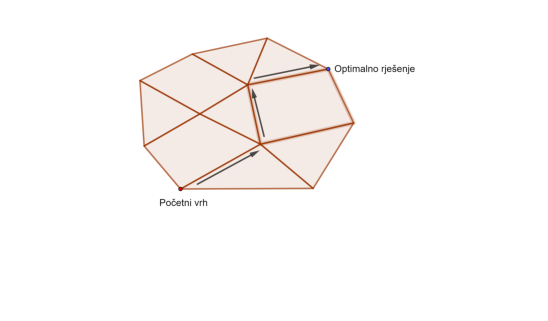
\includegraphics[scale=1.5]{simpleks_move.eps}\vspace{-2cm}
%    \caption{Iteracije simpleks metode (vizuelizacija).}
%    \label{fig:simpleks-visuelisation}
%\end{figure}
%\fxnote{i ja se slazem da nam je ova slika malo bez veze}

 \section{Tabelarni oblik simpleks metoda}


 Simpleks algoritam podrazumijeva stalnu zamjenu jedne kolone baze $B$ nekim nebaznim vektorom u iterativnoj šemi, u cilju smanjenja trenutne vrijednosti ciljne funkcije, dok god je to moguće. 
 U praktičnom računanju, za simpleks metodu se zbog kompaktnosti zapisa,  umjesto transformisanja standardnog oblika LP-a, obično koristi tabelarni prikaz.
 Generički tabelarni  prikaz simpleks metode se može vidjeti u Tabeli~\ref{tab:simplex_tabelau}. Ovakva tabela se naziva  simpleks tabela.

\begin{table}[!ht]
	\centering
	\begin{tabular}{c c c | c} \\ \hline
		$\mid$          &       $\mid$ &  $\mid$             &    $x_{p_1} = \overline{b_1}$         \\
		$B^{-1}A_1$       &    $\cdots$    &  $B^{-1}A_n$      &    $\vdots$          \\
		$\mid$          &       $\mid$ &  $\mid$             &   $ x_{p_m} = \overline{b_m}$         \\ \hline
		$\overline{c_1}$  &    $\cdots$    & $\overline{c_n}$  &  $-c^T_B x_B$         \\ \hline
	\end{tabular}
	\caption{Simpleks tabela}
	\label{tab:simplex_tabelau}
\end{table}

Na osnovu generičke Tabele~\ref{tab:simplex_tabelau} i koraka simpleks metode opisanih u prethodnoj sekciji, izvršavaju se sljedeći koraci:
 \begin{itemize}
	\item Konstruisati inicijalnu simpleks tabelu sa početnom bazom $B$ i  odgovarajuće bazno dopustivo rješenje $x$.
	 \item Posmatrati koeficijente doprinosa $\overline{c_j}$ (posljednja vrsta tabele). Ako su svi $\overline{c_j} \geq 0$, rješenje se ne može dalje popraviti, pa je nađeno optimalno rješenje. U protivnom, odabrati neki indeks $j$ za koji je $\overline{c_j}<0$.
	 \item Posmatrati vektor (kolonu) $u = B^{-1}A_j$. Ako su sve koordinate vektora $u$ negativne, rješenje LP-a je $-\infty$ (funkcija cilja neograničena), algoritam završava sa radom.
	 \item Za svaki $u_i > 0$, računati $x_{p_i}/u_i$, i neka je   ovaj količnik najmanji za indeks $l$. Kolona $A_{j}$ se uključuje u bazu, dok se kolona $A_{p_l}$ isključuje iz baze. 
	 \item Svakom redu simpleks tabele dodati $l$--ti red (pivot red) kojeg množimo odgovarajućim
	 skalarom da bi pivot element (tj. element u presjeku $l$-te vrste i $j$-te kolone) postao 1, a svi ostali elementi u pivot koloni 0.
 \end{itemize}

 U ovom postupku  može se desiti situacija da postoje dva ili više redova koji su kandidati za uključivanje u bazu. Ako se odabere nepovoljan kandidat, postupak može da proizvede degenerativno BDR ili čak da dovede do ciklusa. 
 Da bi se to spriječilo, Robert Bland (1977. godine) je uveo pravilo za pivotiranje danas poznato pod
 nazivom \emph{Blandovo pravilo} koje glasi:
 \begin{enumerate}
 	\item   Među svim nebaznim promjenljivima koje su pogodne za uključivanje u bazu odaberemo onu najmanjeg indeksa. 
 	\item Među svim baznim promjenljivima koje su pogodne za isključivanje iz baze odaberemo onu sa najmanjim indeksom.
 \end{enumerate}
 Može se pokazati da se poštovanjem ovih pravila   simpleks metoda sigurno završava u konačno mnogo koraka. Treba napomenuti da Blandovo pravilo nije jedino pravilo za izbjegavanje ciklusa. Postoji i leksikografsko pravilo pivotiranja koje, zbog konciznosti, ne objašnjavamo ovdje.  

 Obratimo pažnju da se problem minimizacije vrlo lako prevodi u problem maksimizacije sljedećom transformacijom
 $$ \min_{ x \in P} f(x) = - \max_{x \in P}(-f(x)).$$ 
 Prema tome, ako  problem maksimizacije rješavamo simpleks metodom, koraci metoda ostaju isti. Jedina izmjena je u koraku 2, gdje se mijenja znak nejednakosti, jer se mijenja znak koeficijenata u funkciji cilja.  Dakle, posmatraju se indeksi $j$ za koje je $\overline{c_j} > 0$.

\section{Primjena simpleks metoda}
%Kako je standardni poliedar LP-a dat sa svim onim $x \in \mathbb{R}^n$ tako da $Ax \leq (\geq) b$, 
 Transformišimo standardni oblik problema LP-a
\begin{align*}
 	& \max c^T x  \\
 	& {t.d} \nonumber \\
 	& Ax \leq b \\
 	& x \geq 0\\
 \end{align*}
 na kanonski oblik pogodan simpleks metodi $(A {x} = b)$ dodavanjem ,,izjednačavajućih'' promjenljivih $s$ na sljedeći način:
 \begin{align}
 	&  \max  c^T x   \\
 	& Ax + s =  b \\
 	& x \geq 0, s \geq 0. \\
  \end{align}
  što u matričnom obliku odgovara zapisu
 \begin{align}
 	& \max c^T x  \\
 	& (A | I) \cdot \left (\begin{array}{c}
  		x  \\
 		s 
 	\end{array} \right ) =  b \\
 	& (x, s) \geq 0. \\
 \end{align} 

\begin{primjer}\label{primjer:simpl1} Neka je dat problem LP-a:
	\begin{align*}
		&f= \max x_1 + x_2  \nonumber \\
		& t.d. \\
		& x_1 + 3 x_2 \leq 9 \nonumber \\
		& 2x_1 + x_2 \leq 8  \nonumber \\
		& x_1, x_2 \geq 0. \nonumber \\
	\end{align*}
\end{primjer}
\emph{Rješenje.}
Pretvorimo model u kanonski oblik dodavajući izjednačavajuće promjenljive $s = (s_1, s_2)\geq 0$, pa dobijamo 
\begin{center}
	\begin{tabular}{llllll}
		\centering
		& $x_1$    & + $3x_2$  &+ $s_1$ & &= 9 \\
		& $2 x_1$ &   + $x_2$  & + $s_2$ & &= 8 \\
		& $x_1$   &   + $x_2$  &\  & &= $f - 0$ \\
	\end{tabular} 
\end{center}

Ovaj problem odgovara simpleks tabeli \\
\begin{table}[H]
	\centering
	\begin{tabular}{c c c c | c}
		$x_1$ & $x_2$ &  $s_1$ & $s_2$ & \\ \hline
		1 &  3  & 1 & 0 & 9 \\
		2 &  1  & 0 & 1 & 8 \\ \hline
		1 &  1  & 0  & 0 & 0 \\ \hline
	\end{tabular}
	\caption{Inicijalna simpleks tabela.}
	\label{tab:simpleks_tabela1}
\end{table} 

Na početku konstruišimo bazu uzimajući vektore $s_1$ i $s_2$. U tom slučaju, bazno dopustivo rješenje je $x = (0, 0, 9, 8)$, za koje je $f =0$. Sada ažiriramo simpleks tabelu izvodeći pivotiranje. Izaberimo indeks $j$ tako da je  $\overline{c_j}>0$. Neka je $j=1$, odnosno, u razmatranje ćemo uzeti promjenljivu $x_1$, čijim doprinosom želimo da uvećamo funkciju cilja, jer rješavamo problem maksimizacije. Izaberimo pivot vrstu tako što posmatramo odnos $\overline{b_i}/\overline{a}_{1,j}$, za sve $\overline{a}_{1,j} > 0$,  $B^{-1} A_1 = \overline{a}_{1,j}$. Tražimo onaj indeks koji minimizuje datu vrijednost. Imamo dvije mogućnosti, $9/1$ i $8/2$, pa dobijamo da je $i = 2$ traženi indeks. Prema tome, pivot je  element $\overline{a}_{1,2}=2$. Sada izvršimo elementarne operacije pivotiranja oko ovog elementa. Primjenom Gausove metode eliminacije, elemente u koloni 1 simpleks tabele, osim elementa druge vrste,  svedemo na nule, dok element u drugoj vrsti prve kolone postavimo na 1. Vrsti 1 se dodaje druga vrsta pomnožena sa -$\frac{1}{2}$. Druga vrsta se dijeli sa $\frac{1}{2}$. Trećoj vrsti se dodaje druga vrsta pomnožena sa $-\frac{1}{2}$. 
Primjenjujući ove transformacije, dobijamo simpleks tabelu:

\begin{table}[H]
	\centering
	\begin{tabular}{c c c c | c}
		0 &  $\frac{5}{2}$  & 1 & -$\frac{1}{2} $& 5 \\
		1 &  $\frac{1}{2}$ & 0 & $\frac{1}{2}$ & 4 \\ \hline
		0 &  $\frac{1}{2}$ & 0 & -$\frac{1}{2}$ & -4 \\ \hline
	\end{tabular}
	\caption{Simpleks tabela nakon prvog pivotiranja}
	\label{tab:simpleks_tabela2}
\end{table}
Bazne promjenljive sada lako prepoznajemo iz Tabele~\ref{tab:simpleks_tabela2}, jer odgovarajući vektori kolone zajedno formiraju jediničnu matricu. Prema tome, 
nebazne promjenljive su $x_2$ i $s_2$, koje dobijaju vrijednost 0, dok ostale lako izračunavamo, odakle je $ x = (4, 0, 5, 0)$. Ponavljamo prethodne korake nad novom simpleks tabelom. Potrebno je pronaći novi pivot element. Lako se vidi da je jedino kolona 2 odgovarajuća. Pošto je $5 / (5/2) < 4 / (1/2)$, zaključujemo da  pivot element pronalazimo u prvoj vrsti. Dakle, pivot je 
$\overline{a}_{1,2} = \frac{5}{2}$. Postupkom Gausove eliminacije oko prve vrste, dobija se simpleks Tabela~\ref{tab:simpleks_tabela3}.

\begin{table}[!ht]
	\centering
	\begin{tabular}{c c c c | c}
		0 &  $1$  & $\frac{2}{5}$             &  -$\frac{1}{5} $ & 2 \\
		1 &  0    &      -$\frac{1}{5}$    & $\frac{3}{5}$    & 3 \\ \hline
		0 &  0    &   -$\frac{1}{5}$       &   -$\frac{2}{5}$   & -5 \\ \hline
	\end{tabular}
	\caption{Simpleks tabela: korak 2.}
	\label{tab:simpleks_tabela3}
\end{table}
Kako su sve vrijednosti doprinosa manje (ili jednake) 0, zaključujemo da smo pronašli optimum koji je jednak $x = (3, 2, 0, 0)$, a optimalna vrijednost je $f = 5$.

\begin{figure}[!ht]
	\centering
	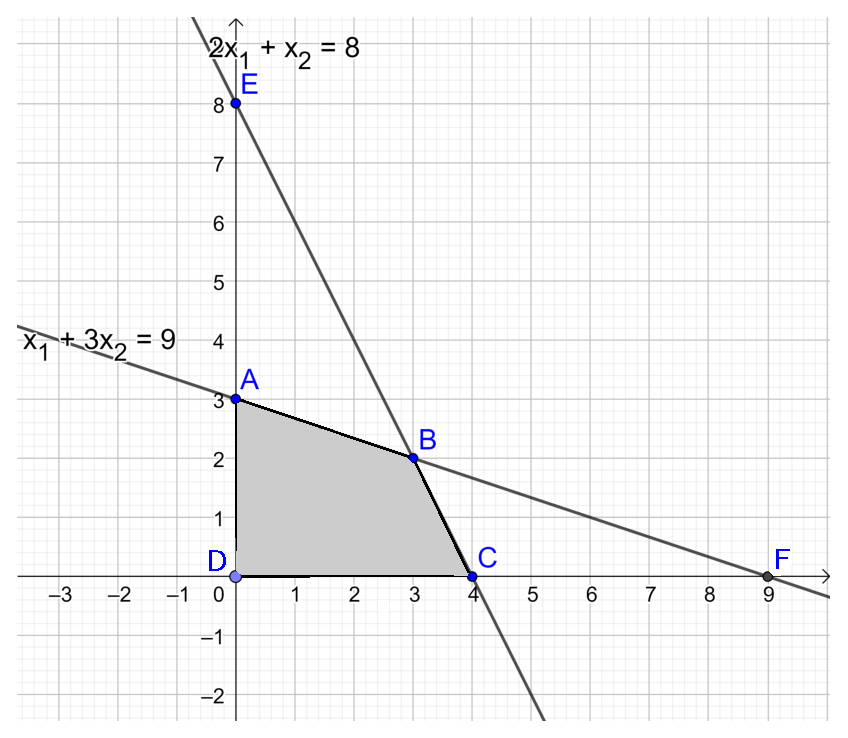
\includegraphics[width=170pt, height=170pt]{simpleks-region-2.eps}
	\caption{Region pretrage (bazna rješenja označena).}
	\label{fig:simplex_region} 
\end{figure}

Analizirajmo još neke aspekte u ovom primjeru. Na Slici~\ref{fig:simplex_region}, tačke $A, B, C$, i $D$ su bazna dopustva rješenja. Tačke $E$ i $F$ su takođe bazna rješenja, ali nisu dopustiva. Simpleks algoritam prvo kreće od tačke $D$ prema tački $C$, te posljednjom iteracijom završava u tački $B$ (optimum).


Iz posljednje simpleks tabele (Tabela~\ref{tab:simpleks_tabela3}) se može uočiti i sljedeće:
\begin{itemize}
	\item Jedinična matrica $m \times m$   ugrađena u gornju lijevu podmatricu simpleks tabele (blok sa elementima $\overline{a}_{i,j}$) sadrži kolone koje čine vektore baznih promjenljivih.
	\item U odgovarajućim kolonama u posljednjoj vrsti (ciljna vrsta) se nalaze nule.
\end{itemize}
Prema tome, vektori $x_i$, koji su bazni (kolone baze $B$), su napisani preko nebaznih vektora $x_i \in N$. Kako je $x_i  = 0$, za sve $i \in N$, vrijednosti baznih vektora $x_i$, tj. kolona baze $B$, se trivijano izračunavaju.

\begin{primjer} Navedimo i primjer jednog linearnog programa koji je neograničen, te ga riješimo simpleks metodom. 
\end{primjer}
Neka je dat problem LP-a:
\begin{align*}
	&\max -x + 3y \\
	&  {\mbox{t.d.}} \nonumber \\
	& -x + y \leq 3 \\
	& x - 2y \leq 2 \\
	& x,y \geq 0.
\end{align*}
Prevedimo problem na kanonski oblik, dodavanjem izjednačavajućih promjenljivih. 
\begin{align*}
	&\max -x + 3y \\
	&  {\mbox{t.d.}} \nonumber \\
	& -x + y + s_1 = 3 \\
	& x - 2y + s_2 = 2  \\
	& (x,s) \geq 0.
\end{align*}
Ovom programu odgovara simpleks tabela:
$$\begin{array}{cccc| c} 
	-1 & 1  & 1 & 0 & 3 \\
	1 & -2 & 0 & 1 & 2 \\ \hline
	-1 & 3  & 0 & 0 & 0  
\end{array}$$

Kako rješavamo problem minimizacije, tražićemo pivota u koloni 2. Jedini kandidat za pivota je element  $\overline{a}_{1, 2} = 1$. Pivotiranjem oko tog elementa dobijamo novu simpleks tabelu 

$$\begin{array}{cccc| c} 
	-1 & 1  & 1  &  0 & 3 \\
	-1 & 0  & 2  &  1 & 8 \\ \hline
	2  & 0  & -3 &  0 & -9 \\
\end{array}$$
Kandidata za pivota tražimo u prvoj koloni. Međutim, kako su svi elementi prve kolone negativni, to znači da se 
vrijednost  promjenljive $x$  može povećavati proizvoljno, odakle slijedi da nije ograničena. 
Grafička reprezentacija dopustivog, neograničenog regiona, prikazana je na  Slici~\ref{fig:unbounded-example-solve}. 


\begin{figure}[!ht]
	\centering
	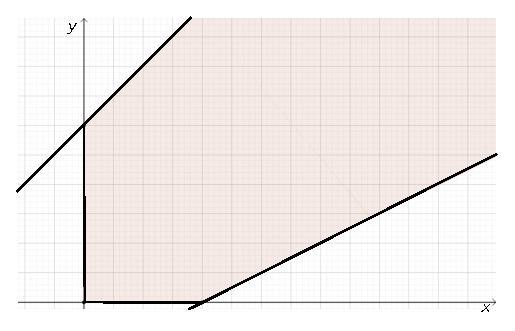
\includegraphics[width=170pt,height=170pt]{unbounded-example-solve.eps}
	\caption{Neograničen region.}
	\label{fig:unbounded-example-solve}
\end{figure}

\begin{primjer} U nastavku dajemo primjer kada pivotiranje u simpleks metodi generiše degenerativno rješenje. 
\end{primjer}
Posmatrajmo sljedeći linearni program:
\begin{align*}
	&\max 2x + 3y \\
	&  {\mbox{t.d.}} \\
	& -x + y \leq 3 \\
	& x - 2y \leq 2 \\
	& x + 6y \leq 18 \\
	& x,y \geq 0. 
\end{align*}
Slično kao i u prethodnom primjeru, dodavanjem izjednačavajućih promjenljivih, dobijamo simpleks 
tabelu 
$$\begin{array}{ccccc|c}
	-1 & 1 & 1 & 0 & 0 & 3 \\
	1 &-2 & 0 & 1 & 0 & 2 \\
	1 & 6 & 0 & 0 & 1 & 18 \\ \hline
	2 & 3 & 0 & 0 & 0 & 0 \\
\end{array}$$
Pretpostavimo smo  za baznu promjenljivu izabrali $y$, tj. pivotiramo oko nekog od elemenata u koloni 2 (zanemarimo ovdje pomenuto Blandovo pravilo odabira pivota). Za pivota odaberemo $\overline{a}_{1,2}=1$ element, te nakon pivotiranja dobijamo novu simpleks tabelu:
$$\begin{array}{ccccc|c}
	-1 & 1 & 1 & 0 & 0 & 3 \\
	-1 & 0 & 2 & 1 & 0 & 8 \\
	7 & 0 & -6 & 0 & 1 & 0 \\ \hline
	5 & 0 & -3 & 0 & 0 & -9 \\
\end{array}$$


Ovdje počinju problemi. Pivotiranje bi trebalo da ide oko nekog elementa u prvoj koloni. Kako tu imamo samo jedan element strogo veći od 0, a to je $\overline{a}_{3,1}=7$, on je ujedno i pivot. Izvršavajući operaciju pivotiranja, promjenljive $\overline{b}$ neće promijeniti svoje vrijednosti, tj. dobijamo sljedeću tabelu:
$$\begin{array}{ccccc|c}
	0 & 1 & \frac{1}{7}  & 0 & \frac{1}{7} & 3 \\
	0 & 0 & \frac{8}{7}  & 1 & \frac{1}{7} & 8 \\
	1 & 0 & -\frac{6}{7} & 0 & \frac{1}{7} & 0 \\ \hline
	0 & 0 & \frac{9}{7}  & 0 & -\frac{5}{7} & -9 \\
\end{array}$$
Geometrijski gledano, razlog za ovakvu situaciju su tri prave $x=0$, $-x+y=3$ i $x+6y=18$ koje se susreću u tački $(0,3)$ (Slika~\ref{fig:deg-sol}). U prošlom koraku, kada su $x$ i $s_1$ bile nebazne promjenljive, tačka (0,3) je posmatrana kao presjek $x=0$ i $-x +y =3$. Nakon sljedećeg koraka $s_1$ i $s_3$ postaju nebazne, pa se pomjeramo u tački presjeka pravih 
$-x+y=3$ i $x+6y=18$, što je opet ista tačka (prema tome, nema ni poboljšanja vrijednosti funkcije cilja). 
Ovo pivotiranje se naziva \emph{degenerativno pivotiranje}. U ovom primjeru, napustićemo vrh $(0,3)$ nakon sljedeće iteracije  pivotiranja. U komplikovanijim primjerima, kada se mnoga ograničenja mogu sresti u jednom vrhu, ostanak u istom vrhu u narednim simpleks koracima je velika opasnost. Ovaj slučaj se može izbjeći poštovanjem 
Blandovog pravila. Primijetimo da koristeći Blandovo pravilo u prvom koraku simpleks metode -- uzimajući za pivota elemente iz kolone 1, a ne kolone 2 --  degenerativno pivotiranje se ne bi pojavilo.  


\begin{figure}[!ht]
	\centering
	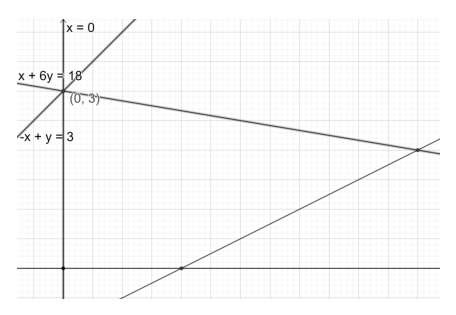
\includegraphics[width=170pt,height=170pt]{deg-sol.eps}
	\caption{Tačka presjeka $(0,3)$ gdje se javlja degenerativno pivotiranje.}
	\label{fig:deg-sol}
\end{figure}

\section{Dvofazni simpleks metod}
Postoje dva pitanja koja se nameću u primjeni simpleks algoritma:
\begin{itemize}
	\item Da li se uvijek (kao i koliko teško)   može naći bazno dopustivo rješenje za inicijalni korak 
	simpleks algoritma?
	\item Da li se simpleks algoritam uvijek prekida pronalaskom optimalnog rješenja ili je funkcija cilja neograničena?
\end{itemize}
Ako postoji jedinična podmatrica $I_m$ u gornjoj lijevoj blok matrici simpleks tabele, onda je jasno da je odgovor na prvo pitanje pozitivan. U primjeru~\ref{primjer:simpl1} su linearnom programu, koji sadrži ograničenja $Ax \leq b, x\geq 0$ pridodate izjednačavajuće promjenljive, kako bi se uslovi nejednakosti u ograničenjima transformirasali u potrebne jednakosti.  Na taj način je formirana i jedinična matrica, pa je i bazu jednostavno odrediti.


Međutim, šta ako je linearan program direktno dat u kanonskom obliku, tj. ograničenjima oblika $Ax = b, x \geq 0$? Bez smanjenja opštosti, pretpostavimo da je $b \geq 0$. Ako ne postoji očigledno bazno dopustivo rješenje ovog problema, onda uvodimo \emph{vještačke} promjenljive (eng. auxiliary variables) $s = (s_1,\ldots, s_m)$. Nakon toga, rješavamo sljedeći problem LP-a:
\begin{align}
	& \min_{x,s} \sum_{i=1}^m s_i  \nonumber \\
	& {\mbox{t.d.}}\label{eq:artificial_lp_simplex}\\
	& A x + s = b \nonumber \\
	&  x, s \geq 0. \nonumber
\end{align}

Postoje dva moguća slučaja:
\begin{enumerate}
	\item Ako početni problem LP-a sa uslovima koji su jednakosti (\ref{eq:lp_equality_constraint}) 
	ima optimalno rješenje, onda   rješenje LP-a (\ref{eq:artificial_lp_simplex}) ima (optimalno) rješenje $s = 0$. 
	\item Ako  (\ref{eq:lp_equality_constraint}) nema dopustivo rješenje, onda je barem jedan $s_i > 0$.
\end{enumerate}
Prema tome, kada  prvo riješimo  problem LP-a  (\ref{eq:artificial_lp_simplex}) simpleks metodom, možemo da zaključimo:
\begin{itemize}
	\item Ako se desio slučaj 2, odustajemo od daljeg rješavanja problema.
	\item Ako se desio slučaj 1, optimalno rješenje problema (\ref{eq:artificial_lp_simplex}) sa $s_i=0$ nam daje početno bazno dopustivo rješenje problema (\ref{eq:lp_equality_constraint}) u prvom simpleks koraku, a, prema tome, i bazne vektore. 
\end{itemize} 
Ovaj korak nas vodi ka \emph{dvofaznoj simpleks metodi}. U nastavku je prikazan primjer kako se problem linearnog programiranja rješava primjenom ove metode.      

% \section{Primjena dvofaznog simpleks metoda}     


\begin{primjer} Primjenom dvofaznog simpleks metoda riješiti sljedeći problem LP-a:
\end{primjer} 

\begin{align*}
	&\min x_1 + x_2 - x_3 - x_4 \\
	& {\mbox{t.d.}} \\
	&x_1 + 2x_2 + x_3 + x_4 = 7 \\
	& 2x_1 - x_2 - x_3 - 3x_4 = -1 \\
	& x_1,x_2,x_3,x_4 \geq 0.
\end{align*}

Dodajmo vještačke promjenljive na početni problem, uz prethodno množenje ograničenja 2 sa (-1), odakle dobijamo:

\begin{align*}
	&\min x_1 + x_2 - x_3 - x_4 \\
	&\mbox{t.d.} \\
	&x_1 + 2x_2 + x_3 + x_4 + s_1 = 7 \\
	& -2x_1 + x_2 + x_3 + 3x_4 + s_2 =  1 \\
	& x_1,x_2,x_3,x_4, s_1, s_2\geq 0.
\end{align*}
Prva faza metoda je rješavanje problema 
\begin{align*}
	&\min s_1 + s_2 \\
	&  {\mbox{t.d.}}\\
	& x_1 + 2x_2 + x_3 + x_4 + s_1 = 7 \\
	& -2x_1 + x_2 + x_3 + 3x_4 + s_2 = 1 \\
	& x_1,x_2,x_3,x_4, s_1, s_2\geq 0.
\end{align*}


Formirajmo početnu simpleks tabelu.
$$\begin{array}{cccccc|c}
	1 & 2 & 1 & 1 & 1 &  0 & 7  \\
	-2 & 1 & 1 & 3 & 0 &  1 & 1  \\ \hline
	0 & 0 & 0 & 0 & 1 & 1 &  0  \\
\end{array}
$$
Množeći prvu i drugu vrstu prethodne tabele sa (-1), te sabiranjem sa trećom vrstom, dobijamo tabelu
$$\begin{array}{cccccc|c}
	1 & 2 & 1 & 1 & 1 & 0 & 7 \\
	-2&1  & 1 & 3 & 0 & 1 & 1 \\ \hline
	1 & -3 & -2 & -4 & 0 & 0 & -8 \\ 
\end{array}
$$
Pošto rješavamo problem minimizacije, u prethodnoj tabeli potražimo promjenljivu 
sa negativnim koeficijentom doprinosa. Prva takva promjenljiva je u koloni 2, u kojoj 
i tražimo pivota.  Kako je $\frac{7}{2} > \frac{1}{1}$, slijedi da je 
pivot $\overline{a}_{2,2} = 1$. Izvršimo transformacije, tako što postavimo sve nule u datoj koloni. Dobijamo novu tabelu:

$$ \begin{array}{cccccc|c}
	5 & 0 & -1 & -5 & 1 & -2 & 5 \\
	-2&1  & 1 & 3 & 0 & 1 & 1 \\ \hline
	-5 & 0 & 1 & 5 & 0 & 3 & -5 \\
\end{array}
$$  
Jedini vektor sa negativnim doprinosom u prethodnoj simpleks tabeli je 
onaj koji odgovara prvoj koloni, pa u njoj i tražimo pivota.  
Kako se jedino u prvoj vrsti nalazi pozitivan element, koji odgovara vrijednosti pravca $\frac{5}{5}$, jasno je da je pivot $\overline{a}_{1,1}=5$. Pivotiranjem oko ovog elementa, dobijamo tabelu 
$$ \begin{array}{cccccc|c}
	1 & 0 & -\frac{1}{5}  & -1   &  \frac{1}{5}     & -\frac{2}{5}  & 1                    \\
	0 & 1 & \frac{3}{5}   &  1   &   \frac{2}{5}  & \frac{1}{5}      & 3                   \\ \hline
	0 & 0 & 0            &  0   &   1        & 1                     & 0                                 \\
\end{array}
$$
Kako su koeficijenti doprinosa svi veći ili jednaki 0, našli smo minimum. 
Prema tome, bazno dopustivo rješenje je jednako $(x, s)= (1,3, 0, 0, 0, 0)$. 

Sada nastavljamo dalje sa algoritmom, odnosno sa drugom fazom metoda.  Posljednja simpleks tabela prve faze dvofaznog simpleks metoda se lako transformiše za početni problem: 

\begin{itemize}
	\item posljednja vrsta dobija koeficijente originalne funkcije cilja razmatranog LP-a;
	\item kolone koje odgovaraju promjenljivima $s$ izbrišemo iz simpleks tabele;
	\item ostale elemente tabele ne mijenjamo.
\end{itemize}
Iz ovih koraka, dobijamo simpleks tabelu 

$$ \begin{array}{cccc|c}
	1 & 0 & -\frac{1}{5}     & -1   & 1 \\
	0 & 1 & \frac{3}{5}      & 1    & 3 \\ \hline
	1 & 1 & -1               & -1   & 0 \\
\end{array}
$$
Načinimo sada elementarne transformacije na ovoj tabeli; kandidata za pivota nađimo u 
koloni 3. Jedini element sa pozitivnom vrijednošću je $\overline{a}_{2,3} = \frac{3}{5}$, koji je onda i traženi pivot. 
Vršeći elementarne transformacije oko pivota, dobijamo tabelu 

$$ \begin{array}{cccc|c}
	1   & \frac{1}{3}       & 0             &   -\frac{4}{3}             &   2  \\
	0   & \frac{5}{3}       & 1	           & \frac{5}{3}                 &   5 \\ \hline
	1   & \frac{8}{3}       & 0             &  \frac{2}{3}               &   3  
\end{array}
$$
Pošto su svi doprinosi svi veći od 0,  našli smo optimalnu simpleks tabelu.  Optimalna rješenja su 
$x_1=2, x_3=5$, pa je  optimum jednak -3.

\section{= geometrijskoj interpretaciji simpleks metoda}

Sljedeći primjer demonstrira odgovarajuće geometrijske korake (,,šetanje'') po dopustivom regionu, u skladu sa iteracijama simpleks metode.   %pratiti https://faculty.math.illinois.edu/~mlavrov/docs/482-fall-2019/lecture5.pdf (strana 2 i 3) 
Neka je dat problem:
\begin{align*}
	&\max 2x + 3y \\
	&  {\mbox{t.d.}} \\
	& -x + y \leq 3 \\
	& x - 2y \leq 2 \\
	& 3x + 4y \leq 26 \\
	& x, y \geq 0.
\end{align*}
Dodajmo izjednačavajuće promjenljive u početni LP, odakle dobijamo 
\begin{align*}
	&\max 2x + 3y \\
	& \mbox{t.d.} \\
	& -x + y + s_1 = 3 \\
	& x - 2y + s_2 = 2 \\
	& 3x + 4y + s_3 =  26 \\
	& x, y, s_1, s_2, s_3 \geq 0.
\end{align*}
Inicijalna simpleks 
tabela je data sa
$$\begin{array}{cccccc| c}
	& x & y & s_1 & s_2 & s_3 & \\ \hline
	s_1  & -1 & 1 & 1 & 0 & 0 & 3 \\
	s_2  & 1 & -2 & 0 & 1 & 0 & 2 \\
	s_3  & 3 & 4 & 0 & 0 & 1 & 26 \\ \hline
	-z  & 2 & 3 & 0 & 0 & 0 & 0 \\
\end{array}
$$  
Kao što je već pomenuto, izjednačavajuće promjenljive čine pogodne bazne promjenljive za početak simpleks metode, jer one formiraju jediničnu podmatricu u gornjoj blok matrici 
simpleks tabele. Prema tome, bazno rješenje je
$(x, y, s_1, s_2, s_3) = (0, 0, 3, 2, 26)$, koje je ujedno i dopustivo.
Na Slici~\ref{fig:step-1} je prikazan dopustivi region problema. Nakon prvog koraka, nalazimo se u tački $A=(0,0)$, koja je dopustiva. Trenutna najbolja vrijednost je jednaka 0. 
\begin{figure}[H]
	\centering
	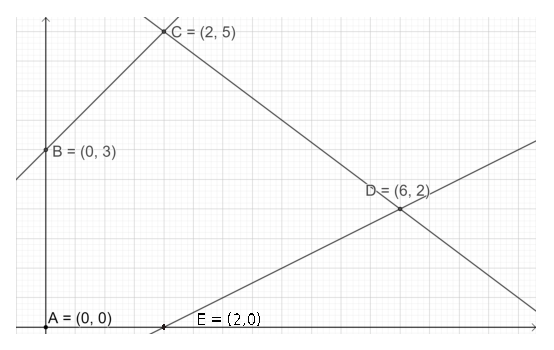
\includegraphics[width=170pt, height=170pt]{simpleks-primjer-2-sl1.eps}
	\caption{Korak 1}
	\label{fig:step-1}
\end{figure}
Izvršimo sada promjenu baznih vektora na osnovu  koraka simpleks metoda. Pošto maksimizujemo, 
tražimo one koeficijente dopirnosa koji su veći od 0. Biramo prvu kolonu, koja odgovara promjenljivoj $x$. Pronađimo 
pivot element: kandidati su $s_2$ i $s_3$.
Kako je $\frac{26}{3} > \frac{2}{1}$, onda je  pivot $\overline{a}_{2, 1} = 1$. Pivotiramo oko ovog elementa i dobijemo tabelu:
$$\begin{array}{cccccc| c}
	& s_2  & y  & s_1  & s_2 & s_3 &    \\ \hline
	s_1 & 0    & -1  & 1  & 1 & 0  &  5     \\
	x   & 1    & -2  & 0  & 1 & 0  &  2     \\
	s_3 & 0    & 10   &  0  & -3 & 1 & 20   \\ \hline
	-z  & 0    &  7   & 0   & -2 & 0 & -4   \\ 
\end{array}
$$ 
Ova tabela vizuelno odgovara Slici~\ref{fig:step-2}. Prelazi se u bazno rješenje $(x,y, s_1, s_2, s_3)=(2, 0, 5, 0 ,20)$, odnosno do tačke $E=(2, 0)$. 

\begin{figure}[!ht]
	\centering
	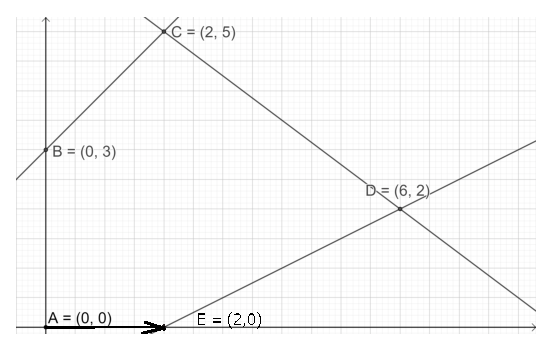
\includegraphics[width=170pt, height=170pt]{simpleks-primjer-2-sl2.eps}
	\caption{Korak 2}
	\label{fig:step-2}
\end{figure}
Dalje, narednog pivota nalazimo u drugoj koloni, koja odgovara promjenljivoj $y$. Jedini kandidat za pivota je element $\overline{a}_{3, 2}= 10$, pa nakon pivotiranja dobijamo tabelu 
$$\begin{array}{cccccc| c}
	& s_2  & s_3   & s_1  & s_2 & s_3 &     \\ \hline
	s_1 & 0    &  0    & 1    &  \frac{7}{10}  & \frac{1}{10} &   7  \\  
	x   & 1    &  0    & 0    &  \frac{2}{5}   & \frac{1}{5}  &   6  \\
	y   & 0    &  1    & 0    & - \frac{3}{10}  & \frac{1}{10} &   2  \\ \hline
	-z  & 0    &  0    & 0    &   \frac{1}{10} &-\frac{7}{10}  &  -18 \\ 
\end{array}
$$ 

\begin{figure}[H]
	\centering
	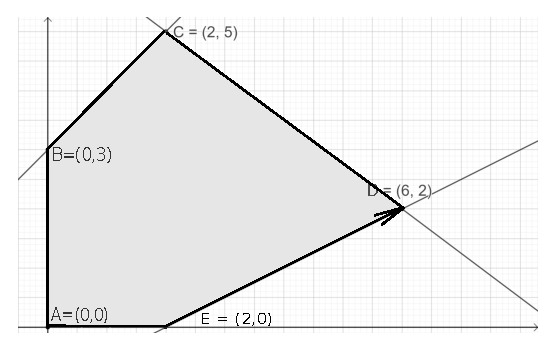
\includegraphics[width=170pt, height=170pt]{simpleks-primjer-2-sl3.eps}
	\caption{Korak 3}
	\label{fig:step-3}
\end{figure}

Ova tabela odgovara kretanju od tačke $E=(2,0)$ do tačke $D=(6,2)$, što je i prikazano na Slici~\ref{fig:step-3}.
Zaključujemo da je jedina koordinata koja odgovara pozitivnom doprinosu kolona 
4 simpleks tabele. Pivotiranje vršimo oko elementa $\overline{a}_{1,4} = \frac{7}{10}$ i  dobijamo simpleks tabelu 

$$\begin{array}{cccccc| c}
	& s_2  & s_3   & s_1  & s_2 & s_3 &     \\ \hline
	s_2 &  0   &  0    & \frac{10}{7}    &  1   & \frac{1}{7}   & 10 \\
	x   &  1   &  0    &  \frac{4}{7}    &  0   & \frac{1}{7}  & 2 \\
	y   &  0   &  1    &  \frac{3}{7}    &  0   & \frac{1}{7}   & 5  \\ \hline
	-z  &  0   &  0   &   -\frac{1}{10}  & 0    &  -\frac{5}{7} & -19 \\
\end{array}
$$ 

Kako ne postoje koordinate čiji su doprinosi pozitivni, našli smo optimum, koji se dostiže u tački $C=(2,5)$. Prethodna simpleks tabela odgovara Slici~\ref{fig:step-4}, dok sve iteracije u simpleks metodi odgovaraju putanji $A \rightarrow E \rightarrow D \rightarrow C$. 

\begin{figure}[H]
	\centering
	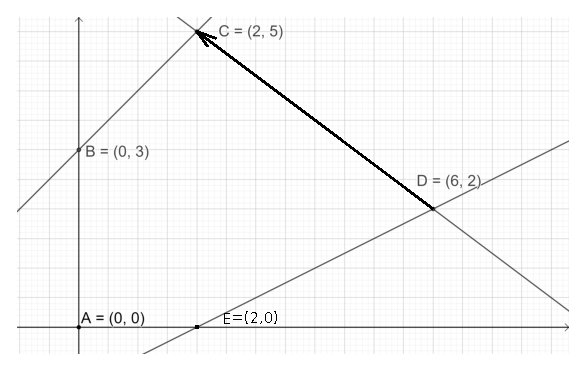
\includegraphics[width=170pt, height=170pt]{simpleks-primjer-2-sl4.eps}
	\caption{Korak 4}
	\label{fig:step-4}
\end{figure}


U slučaju da smo, u prvom koraku simpleks metode, umjesto promjenljive $x$ u bazu uključili promjenljivu $y$, do optimuma bismo došli pomjeranjem u tačku $B$, a potom u tačku $C$, koja je i optimum. U ovom slučaju bi bilo potrebno generisati samo dvije simpleks tabele (a ne tri, kao što smo imali u ovom primjeru).
\\
\section{Zadaci}
\begin{enumerate}
	\item Uz pomoć Simpleks metoda, riješiti sljedeći problem LP-a:%http://www.phpsimplex.com/en/simplex_method_example.htm (PHP simpleks: http://www.phpsimplex.com/simplex/simplex.htm?l=en)
	\begin{align*}
		&\max  3x + 2y \\
		& \mbox{t.d.} \\
		& 2x + y \leq 18 \\
		& 2x + 3y \leq 42 \\
		& 3x + y \leq 24 \\
		& x,y \geq 0.
	\end{align*} 
	Uporedite dobijeno rješenje sa rješenjem koje se dobije 
	koristeći grafičku metodu.
	\item %https://courses.lumenlearning.com/sanjacinto-finitemath1/chapter/reading-solving-standard-maximization-problems-using-the-simplex-method/
	Koristeći simpleks metodu, riješiti sljedeći problem LP-a:
	\begin{align*}
		&\max 2x + 3y + z \\
		&   {\mbox{t.d.}} \\
		& 3x + 5 y \leq 5 \\
		& 2x + y - z \leq 13 \\
		& z \leq 4 \\
		& x,y,z \geq 0.
	\end{align*}
	\item Uz pomoć dvofaznog simpleks metoda, riješiti sljedeći problem LP-a:%http://sma.epfl.ch/~niemeier/opt09/opt09_ch06.pdf
	\begin{align*}
		&\min  x_1 + x_2 + x_3 \\
		& {\mbox{t.d.}} \\
		& x_1 + 2 x_2 + 3 x_3 = 3 \\
		& -x_1 + 2 x_2 + 6 x_3 = 2 \\
		& - 4x_2 - 9 x_3 = -5 \\
		& 3 x_3 + x_4 = 1 \\
		& x_1, x_2, x_3, x_4 \geq 0.
	\end{align*}
	\item  Uz pomoć simpleks metoda, riješiti sljedeći problem LP-a:%http://myweb.usf.edu/~molla/2016_spring_math482/two_phase_pres-3up.pdf
	\begin{align*}
		& \min -x_1 - x_2 - x_3 \\
		&  {\mbox{t.d.}} \\
		& 2 x_1 - x_2 + 2 x_3 + x_4 = 4 \\
		& 2x_1 - 3x_2 + x_3 + x_5 =  -5 \\
		& -x_1 + x_2 - 2x_3 + x_6 = -1 \\
		& x_1, x_2, x_3, x_4, x_5, x_6 \geq 0.	
	\end{align*}
	\item Uz pomoć simpleks metoda, riješiti sljedeći problem LP-a:
	%https://personal.utdallas.edu/~scniu/OPRE-6201/documents/LP10-Special-Situations.pdf (Degeneracy in Simplex method):
	\begin{align*}
		&\max 2x_1 + x_2 \\
		&   {\mbox{t.d.}} \\
		&4 x_1 + 3 x_2 \leq 12 \\
		& 4 x_1 + x_2 \leq 8 \\
		& 4 x_1 + 2 x_2 \leq 8 \\
		& x_1, x_2 \geq 0.
	\end{align*}
	Da li se u nekom koraku simpleks metode javlja degenerativno bazno rješenje? Ako je to slučaj, diskutovati zašto je ono degenerativno. 
	\item Iako je simpleks metod u prosječnom slučaju efikasan metod za rješavanje LP problema, u najgorem slučaju, vrijeme izvršenja eksponencijalno zavisi od broja vrhova dopustivog skupa. Koristeći pouzdane internet izvore, pronađi i analiziraj primjer LP problema sa $D$ promjenljivih i $D$ ograničenja, kod koga simpleks metod obilazi svih $2^D$ vrhova politopa. Jedan od primjera takvog politopa je tzv. Kli-Mintijeva kocka (eng. Klee-Minty cube).
	
\end{enumerate}


\begin{comment}
	$$\begin{array}{ccccc}
		\max                & 3x_1     &          &   + x_3  &       \\           
		{s.t. }   & x_1      &+ 2x_2    &   + x_3  & = 30  \\
		& x_1      &- 2x_2    &   + 2x_3 & = 18  \\
		& x \geq 0 &          &       &          \\
	\end{array}$$
	Dodavanjem umjetnih varijabli, dobijamo problem
	
	$$\begin{array}{ccccccc}
		\min                &          &          &            & \omega_1 & +\omega_2   &    \\           
		{s.t. }  & x_1      &+ 2x_2    &   + x_3    &+ \omega_1  &  &= 30  \\
		& x_1      &- 2x_2    &   + 2x_3    & & \omega_2  &= 18  \\
		& x \geq 0 &  \omega \geq 0        &       &    &  &     \\
	\end{array}$$
	
	Problem minimizacije se može prebaciti na problem maksimizacije, tj. prvi uslov u prethodnom problemu prevedemo na $\max - \omega_1 - \omega_2$, što onda odgovara simpleks tabeli 
	
	$$\begin{array}{ccccc | c}
		1 & 2   & 1 & 1 & 0   & 30 \\
		1 & -2  & 2 & 0 & 1   & 18 \\ \hline
		0 & 0   & 0 & -1 & -1 & 0 \\
	\end{array}$$
	Prvo što trebamo da izrazimo funkciju cilja preko nebaznih varijabli tako da ulazi ispod jedinične matice budu svi 0. To dobijamo elementarnim transformacijama na simpleks tabeli (matrici): vrsti 3 dodamo vrstu 1 i 2, te dobijamo tabelu 
	
	$$\begin{array}{ccccc | c}
		1 & 2   & 1 & 1 & 0   & 30 \\
		1 & -2  & 2 & 0 & 1   & 18 \\ \hline
		2 & 0   & 3 & 1 & 1   & 48 \\
	\end{array}$$
	Krenimo sa simpleks koracima, tj. nađimo pivota. Kandidat je $\overline{a}_{2,3}$, pa pivotirajmo oko tog elementa, čime dobijamo tabelu 
	
	$$\begin{array}{ccccc | c}
		\frac{1}{2} & 3   & 0 &  1 &  -\frac{1}{2} & 21 \\
		\frac{1}{2} & -1  & 1 & 0 & \frac{1}{2}   & 9 \\ \hline
		\frac{1}{2} & 3   & 0 & 0 &  -\frac{3}{2}  & 21 \\
	\end{array}$$
	Dakle, sljedeći pivot je $\overline{a}_{1,2}$, gdje nakon pivotiranja dobijamo sljedeću tabelu 
	
	$$\begin{array}{ccccc | c}  
		\frac{1}{6} & 1   & 0 &  \frac{1}{3} &  -\frac{1}{6} & 7 \\
		\frac{2}{3} & 0  & 1 & \frac{1}{3} & \frac{1}{3}   & 16 \\ \hline
		0 & 0   & 0 & -1 &  -1  & 0 \\
	\end{array}$$
	Prema tome, našli smo tačku tako da je $-\omega_1 - \omega_2 = 0$, dakle slijedi 
	da je bazna dopustiva tačka početnog problema $x = (0, 7, 16)$. 
	
	Sljedeći korak sadrži primjenu simpleks metoda na originalni problem.
	Posljednja simpleks tabela prve faze dvofaznog simpleks metoda se lako transformiše za početni problem: 
	\begin{itemize}
		\item posljednja vrsta dovija koeficijente originalne funkcije cilja razmatranog LP-a:
		\item kolone koje odgovaraju varijablama $\omega$ izbrišemo iz simpleks tabele;
		\item ostale elemente tabele ostavimo kakvi jesu.
	\end{itemize}
	Iz ovih koraka, dobijamo simpleks tabelu 
	$$
	\begin{array}{ccc|c}
		\frac{1}{6}       & 1   & 0  & 7   \\
		\frac{2}{3}       &  0   & 1  & 16  \\ \hline
		3                 & 0   & 1  & 0   \\
	\end{array}
	$$
	Opet je potrebno ispod jedinične matrice u vrsti koja odgovara funkciji cilja napraviti nule. To uradimo primjenjujući elementarne transformacije na matrici, tj. vrsti 3 dodamo vrstu 2 koja je pomnožena sa -1. Tada dobijamo simpleks matricu 
	
	$$
	\begin{array}{ccc|c}
		\frac{1}{6}       & 1   & 0  & 7   \\
		\frac{2}{3}       &  0   & 1  & 16  \\ \hline
		\frac{7}{3}                 & 0   & 0  & -16  \\
	\end{array}
	$$
	Za pivota uzmemo $\overline{a}_{2, 1}$, izvršimo transformacije i dobijemo tabelu 
	$$
	\begin{array}{ccc|c}
		0       & 1    & -\frac{1}{4}  & 3   \\
		1       &  0   & \frac{3}{2} & 24  \\ \hline
		0       &  0   & -\frac{7}{2}  & -72 \\
	\end{array}
	$$
	Kako su svi koeficijenti doprinosa ($\overline{c}$ varijable) manje od 0, simpleks metod staje nalazeći optimum koji se dostiže u tački $x = (24, 3, 0)$, i jednak je vrijednosti  $f = 72$.
\end{comment}
% \newpage

 \chapter{Dualnost i dopustivost}\label{chp:dualnost}

%Dualnost je pojam koji je vezan za dobijanje gornjih granica optimalne vrijednosti funkcije cilja. 
 U teoriji linearnog programiranja, ali i teoriji optimizacije uopšte, pod dualnošću podrazumijevamo da se neki problem može posmatrati s dva različita aspekta: kao primalni i kao dualni problem. 
 Preciznije, teorija dualnosti povezuje dva problema linearnog programiranja -- jedan od njih je problem linearnog programiranja koji maksimizuje funkciju cilja, dok je drugi linearan program  koji minimizuje (ne obavezno istu) funkciju cilja.  Na osnovu istih ulaznih podataka, svaki problem LP-a se može navesti u drugom, ekvivalentnom obliku. Ponekad rješavanje dualnog problema LP-a može da bude puno lakše nego rješavanje početnog problema.  Dualnost implicira da svaki problem linearnog programiranja možemo analizirati na dva potpuno različita načina, ali sa ekvivalentnim (optimalnim) rješenjima. 

U ovom poglavlju ćemo najprije objasniti kako se od početnog, primarnog problema formira dualni problem. Nakon toga, biće navedene Teoreme o slaboj i jakoj dualnosti, koje daju vezu između rješenja i ograničenja primarnog i dualnog problema. U nastavku poglavlja su objašnjene još neke važne tehnike koje se koriste za rješavanje problema linearnog programiranja: Farkašova lema i Furije-Mockinova eliminacija. Dodatno, metod unutrašnje tačke će biti dat u Dodatku A. 

Prije nego što uvedemo pojam dualnog problema, objasnimo motivaciju koja stoji iza nastanka teorije dualnosti.

\begin{primjer}  
	Posmatrajmo jedan LP i probajmo naći što bolju gornju procjenu za optimalnu vrijednost  funkcije cilja na osnovu ograničenja u datom modelu.
\end{primjer}

$$ 
\begin{array}{lllll}  
	\max                f((x_1,x_2))=  &x_1 &+& x_2   &               \\
	\mbox{t.d.}  &4x_1 & +&3 x_2 & \leq 9        \\
	&x_1 &+ &x_2   &  \leq 8       \\
	&x \geq 0  &  &     &      
\end{array}
$$
Iz uslova je jasno da su gornje granice date sa $f(x_1,x_2) = x_1 + x_2 \leq 4 x_1 + 3 x_2 \leq 9$, kao i 
$f(x_1,x_2) \leq x_1 + x_2 \leq 8$. Gornje granice se mogu i poboljšati na osnovu sljedećeg niza nejednakosti
$$f(x_1,x_2) \leq \frac{1}{4}(  4 x_1 + 3 x_2  ) + \frac{1}{4}(    x_1 +   x_2 ) = \frac{5}{4}x_1 + x_2 \leq  \frac{9}{4} + 2 = \frac{17}{4},$$ 
čime dobijamo bolju gornju granicu vrijednosti funkcije $f$. 

Izvedimo sada ovakvu konstrukciju u opštijem obliku. Iskoristimo ograničenja data u modelu, i iskombinujmo ih sa koeficijentima funkcije cilja na sljedeći način. Neka su $y_1, y_2 \geq 0$ koeficijenti sa kojima množimo ograničenja u početnom modelu. Tada imamo 
\begin{align*}
	&y_1 \cdot (4x_1 + 3x_2) \leq 9 y_1 \\
	&y_2 \cdot (x_1 + x_2 ) \leq 8 y_2 
\end{align*}
Sabirajući ove dvije nejednakosti i grupišući sabirke dobijamo 
\begin{equation}\label{eq:dual-1}
	x_1 ( 4 y_1 + y_2 ) + x_2 ( 3 y_1 + y_2 ) \leq 9 y_1 + 8 y_2 
\end{equation}
Posmatrajući funkciju cilja i koeficijente uz promjenljive u (\ref{eq:dual-1}), jasno je da treba da vrijedi 
$4 y_1 + y_2 \geq 1$ i $3 y_1 + y_2 \geq 1$. Da bi ocjena gornje granice   izraza sa lijeve strane nejednakosti (\ref{eq:dual-1}) bila što bolja,   potrebno je minimizovati izraz $9y_1 + 8 y_2$, prema prethodno pomenuta (dva) uslova. Prema tome, početnom problemu, koji označavamo sa ($P$), odgovara dualni problem ($D$)
 $$\begin{array}{ll}
	\min                    &  9 y_1+ 8 y_2        \\
	\mbox{t.d.}   &  4 y_1     +   y_2 \geq 1   \\
	&  3 y_1 + y_2 \geq 1 \\
	&            y=(y_1,y_2) \geq 0.
 \end{array}$$
U opštem slučaju,  za problem ($P$) %~(\ref{eq:LP-o1})--(\ref{eq:LP-c2}), 
\begin{align*}
	& \max c^T x  \\
	& \mbox{t.d.} \nonumber \\
	& A x \leq b \\
	& x \geq 0.
\end{align*}
odgovorarajući dualni problem ($D$)  je dat sa 
\begin{align*}
	& \min b^T y  \\
	& \mbox{t.d.} \nonumber \\
	& A^T y \geq c \\
	& y \geq 0.
\end{align*}

\section{Teoreme dualnosti}
U ovom odjeljku ćemo navesti najvažnije teoreme koje omogućavaju primjenu teorije dualnosti na rješavanje problema linearnog programiranja.

\begin{thm}[Teorema slabe dualnosti]
	Ako je x dopustivo rješenje za problem ($P$) i y dopustivo rješenje za problem  ($D$), onda je 
	$$ c^T x \leq b^T y.$$
\end{thm}
\begin{proof}
	Kako je $A^T y \geq c $,  transponovanjem obje strane dobijemo 
	$y^T A \geq c^T$. Množenjem obje strane posljednje nejednakosti sa $x \geq 0$, dobijamo 
	$$y^TAx \geq c^T x.$$ Kako je $Ax \leq b$ i $y \geq 0$,  tada dobijamo 
	$ y^T b = b^T y  \geq c^T x$
\end{proof}
Iz Teoreme slabe dualnosti slijedi sljedeća važna posljedica.
\begin{poslje}
	Ako je $y$ dopustivo rješenje problema  ($D$),  onda bilo koje dopustivo rješenje $x$ problema ($P$) je ograničeno odozgo sa $b^T y$. Prema tome, ako je problem ($D$) dopustiv, onda je ($P$) ograničen. Slično se može pokazati da vrijedi i obrnuto,  kada problemi ($P$) i ($D$) zamijene uloge.
\end{poslje}

Pokažimo da važi i naredno tvrđenje, koje ćemo koristiti u dokazu Teoreme jake dualnosti.

\begin{prop}  
	Ako je $x^*$ dopustivo rješenje za  ($P$), $y^*$ dopustivo rješenje za ($D$) i ako vrijedi   	$c^T x^* = b^T y^*$, onda je $x^*$ optimalno rješenje za problem  ($P$), a $y^*$ optimalno rješenje za problem  ($D$).  
\end{prop}
\begin{proof}
	Neka je $x$ bilo koje dopustivo rješenje problema ($P$). Iz teoreme o slaboj dualnosti imamo $c^T x  \leq b^T y^* = c^T x^*$, odakle slijedi da je $x^*$ upravo optimalno rješenje problema  ($P$).
	Slično vrijedi i za sva dopustiva rješenja problema ($D$): $b^T y^* = c^T x^* \geq b^T y$, odakle imamo da je $y^*$ optimalno rješenje problema  ($D$). 
\end{proof}

\begin{thm}[Teorema jake dualnosti]
	Ako problem ($P$) ima optimalno rješenje $x^*$, onda i problem ($D$) ima optimalno rješenje $y^*$ i pri tome je $c^T x^* = b^T y^*$.
\end{thm}
\begin{proof}
	Napišimo ograničenja probema ($P$) kao $Ax + s = b, x, s \geq 0$.
	Primijenimo simpleks metod, pa posmatrajmo posljednju  simpleks tabelu, odnosno tabelu iz koje se dobija rješenje $x^*$.
	
	$$\begin{array}{c |c | c}
		\overbrace{\ \ \ \ \ \hspace{1.5cm}}_{x \mbox{ promjenljive}}     &  \overbrace{\ \ \ \ \ \hspace{1.5cm}}_{s \mbox{ promjenljive}} &   \\
		& &   \\
		\hline
		c_1^*\ c_2^* \ldots c_n^*            & -y_1^* -y_2^* \ldots -y_m^*  & -f^*
	\end{array}
	$$
	gdje je 
	\begin{enumerate}
		\item    $c^*_i \leq   0, i = 1,\ldots, n$ 
		\item    $-y_i^* \leq 0$, $i = 1,\ldots, m$
		\item  $c^T x - f^* = (c^*)^T x - (y^*)^T s$ (iz koeficijenata doprinosa simpleks metode)
	\end{enumerate}
	Prema tome, 
	\begin{align*}
		c^T x &=  f^* + (c^*)^T x - (y^*)^T s \\
		&=  f^* + (c^*)^T x - (y^*)^T (b - Ax) \\
		&= f^*  - (y^*)^T b +   ((c^*)^T + (y^*)^T A ) x
	\end{align*}
	koje vrijedi za sve $x$. Specijalno, za  $x = 0$,  dobijamo 
	
	\begin{equation}\label{eq:f_y_star}
		f^* = (y^*)^T b.
	\end{equation}
	
	Dalje, važi i $c^T x = ((c^*)^T + (y^*)^T A ) x$, odnosno     $ c = A^T y^* + c^*$. 
	
	Kako je $c^* \leq 0$, imamo  $A^T y^* \geq c$. Kako je $-y^* \leq 0$, slijedi da je $y^*$ dopustivo rješenje za  ($D$).  Iz (\ref{eq:f_y_star}) imamo da je vrijednost funkcije cilja u $y^*$ upravo $f^* = c^T x^* $. Iz Propozicije 5.1  slijedi da je $y^*$ optimalno rješenje problema  ($D$). 
	
	
\end{proof} 

Primijetimo da koeficijenti $y^*$ posljednje vrste završne simpleks tabele odgovaraju  ,,izjednačavajućim''   promjenljivima i one nam daju rješenje problema  ($D$).  

\begin{primjer} Moguće je da problem ($P$) i njegov   dual ($D$) nemaju dopustivo rješenje. Pogledajmo sljedeći primjer:
\end{primjer}
$$\begin{array}{cc}
	\max          & 2 x_1 - x_2 \\
	{\mbox{t.d.} }      & x_1 - x_2 \leq 1 \\
	& -x_1 + x_2 \leq -2 \\
	& x_1, x_2 \geq 0.
\end{array}$$
%i pokažite da je to slučaj.
\emph{Rješenje.} Množenjem drugog ograničenja sa -1, dobijamo $x_1 - x_2 \geq 2$, što u kombinaciji sa prvim ograničenjem jasno pokazuje da problem ($P$) nema dopustivih rješenja. Dualni problem ($D$) ovog LP-a je dat sa 
$$\begin{array}{cc}
	\min          &x_1 - 2x_2 \\
	{\mbox{t.d.} }       & y_1 -y_2 \geq 2 \\
	& -y_1 + y_2 \geq -1 \\
	& y_1, y_2 \geq 0.
\end{array}$$
Množeći drugo ograničenje sa -1, dobijamo $y_1 -y_2 \leq 1$, što u kombinaciji sa prvim ograničenjem jasno pokazuje da problem ($D$) nema dopustivo rješenje. ~

Analizirajmo sada i koncept  \emph{komplementarnosti} (eng. \emph{complementary slackness}), koji nam omogućava da uspostavimo još neke važne odnose između promjenljivih i ograničenja primarnog i dualnog problema. 
\begin{thm}[Teorema komplementarnosti]
	
	Neka su $x$ i $y$ dopustiva rješenja problema ($P$) i  ($D$), redom. Vektori $x$ i $y$ su optimalna rješenja ova dva problema akko vrijedi 
	
	\begin{equation}\label{eq:slackness-2} 
		(Ax - b)_i y_i = (a_{i1}x_1 + \cdots + a_{in}x_n - b_i)y_i = 0, i=1,\ldots,m 
	\end{equation} 
	i 
	\begin{equation}\label{eq:slackness-1} 
		(A^Ty - c)_j x_j =  ( a_{1 j}y_1 + \cdots a_{m j}y_m - c_j  ) x_j =  
		0, j=1,\ldots,n 
	\end{equation}    
	
\end{thm} 
Uslovi (\ref{eq:slackness-1}) i (\ref{eq:slackness-2}) se nazivaju \emph{uslovi komplementarnosti}. 

\begin{proof}
	Iz teoreme o slaboj dualnosti imamo:  
	\begin{equation} 
		c^Tx \leq ( A^T y)^T x = y^T A x \leq b^T y.  
	\end{equation} 
	Dalje, iz teoreme jake dualnosti imamo   
	\begin{align*} 
		&x \mbox{ i } y \mbox{ su oba optimalna } \Longleftrightarrow c^T x = b^T y  \Longleftrightarrow c^Tx = y^TA x = b^Ty \\ 
		&\Longleftrightarrow (y^T A - c^T) x = 0 \wedge y^T(Ax - b )  = 0\\ 
		& \Longleftrightarrow \sum_i (A^T y - c)_i x_i = 0 \wedge \sum_j (Ax - b)_j y_j = 0 
	\end{align*} 
	Kako je $A^Ty \geq c$, $\sum_i (A^T y - c)_i x_i$ je suma nenegativnih komponenti, odakle  slijedi da   $(A^T y - c)_i x_i= 0$ za sve $i$. Takođe, slično vrijedi i za drugu sumu, jer $Ax - b \leq 0$, pa je svaki  $(Ax - b)_j y_j$ negativan, odakle slijedi da je $(Ax - b)_j y_j = 0$ za sve $j$.
\end{proof} 

\emph{Komentar}.  Nekada je lakse riješiti jedan od problema, ($P$)  ili  ($D$).  Npr. lakše je riješiti dualni problem sa dvije promjenljive i 4 ograničenja (grafički metod), nego primalni  ($P$)  problem sa 4 promjenljive i 2 ograničenja. 

\begin{primjer} Posmatrajmo primarni  ($P$)  i dualni ($D$) problem, gdje su
\end{primjer}

$$      A = \left(\begin{array}{ccc}
	1 &  4 & 0 \\
	3 & -1 & 1 \\
\end{array} \right ), b = \left (\begin{array}{c}
	1 \\
	3
\end{array}\right ), c =\left ( \begin{array}{c}
	4  \\
	1  \\
	3
\end{array} \right )
$$
Posmatrajmo jedno dopustivo rješenje problema  ($P$), $x = (0, \frac{1}{4}, \frac{13}{4})$. Da li je ono optimalno? Ako bi bilo optimalno,  prema Teoremi komplementarnosti, vrijedilo bi sljedeće:

$$x_2 \geq 0 \Rightarrow  (A^T y)_2  = c_2, \mbox{ tj. } 4 \cdot y_1 - y_2 = 1$$
$$x_3 \geq 0 \Rightarrow  (A^T y)_3  = c_3, \mbox{ tj. } 0 \cdot y_1 + y_2 = 3$$
što nam daje  $y = (1, 3)$. Preostalo ograničenje $y_1 + 3 y_2 \geq 4$ takođe vrijedi za vektor $y$, odakle imamo da je $y$ dopustivo rješenje odgovarajućeg problema  ($D$).  Prema tome, zaključujemo da su $x$ i $y$ dopustiva rješenja koja zadovoljavaju svojstvo komplementarnosti, pa su to i optimalna rješenja. 

\begin{figure}[!ht]
	\centering
	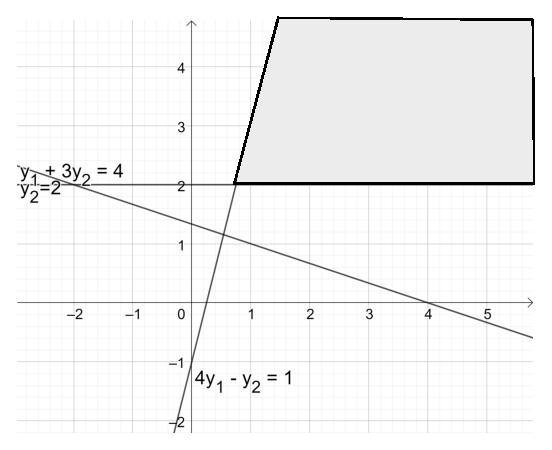
\includegraphics[width=180pt, height=180pt]{fig5.eps}
	\caption{Dualni problem: dopustiv region}
	\label{fig:fig5}
\end{figure}

Optimalno rješenje je u presjeku pravih $y_2 = 3$ i $4y_1 - y_2 = 1$, odnosno $y = (1, 3)$. Provjerimo, pomoću Teoreme komplementarnosti, potencijalne tačke za optimalno rješenje problema ($P$). Imamo 
$$y_1 > 0 \Rightarrow (Ax - b)_1 y_1 = 0 \Rightarrow x_1 + 4 x_2 = 4 $$
$$y_2 > 0 \Rightarrow (Ax - b)_2 y_2 = 0 \Rightarrow 3x_1 - x_2 + x_3 = 3 $$
i kako je $y_1 + 3 y_2 > 4$, onda $(A^Ty)_1 > c_1$ i prema tome $x_1 =0$, 
odakle $x =(0, \frac{1}{4}, \frac{13}{4})$. 

\begin{primjer}\label{primjer:dual} Posmatrajmo problem LP-a
\end{primjer}
$$\begin{array}{llll}
	&\max                     &10 x_1 + 10 x_2 + 20 x_3 + 20 x_4  & \\
	&\mbox{t.d. }      &12 x_1 + 8 x_2  + 6 x_3  + 4 x_4   & \leq 210 \\
	&                        &3 x_1 + 6 x_2   + 12 x_3 + 24 x_4 & \leq 210 \\
	&                       & x_1,\ldots, x_4 \geq 0.                                 &
\end{array}
$$
Ovaj problem ima 4 promjenljive i 2 ograničenja. Prema tome, ima smisla razmatrati dualni problem  ($D$)  datog primala  ($P$),  jer u tom slučaju dobijamo linearni program od samo dvije promjenljive koji se može lako riješiti grafičkom metodom.  Odgovarajući problem ($D$) je dat sa:

$$\begin{array}{lll}
	&\min                    &  210 y_1 + 210 y_2      \\
	&{s.t. }     &  \\
	&            &  12 y_1  + 3   y_2 \geq 10 \\
	&                        &  8  y_1 + 6    y_2 \geq 10 \\
	&                        &  6 y_1 + 12 y_2  \geq 20 \\
	&                        &  4 y_1 + 24 y_2  \geq 20 \\
	&                        &  y_1, y_2 \geq 0.
\end{array}$$
Dopustiv region dualnog problema je dat na Slici~ \ref{fig:fig6-dual-region}. %gdje je dopustiv region označen plavom bojom. 
Dalje, može se pokazati da je optimum duala u presjeku prave $12 y_1 + 3 y_2 = 10$ i prave $6y_1 + 12 y_2 = 20$. Na osnovu Slike \ref{fig:fig6-dual-region} vidimo da   prava koja odgovara drugom i četvrtom ograničenju LP-a mimoilazi tačku optimuma, jer vrijedi stroga nejednakost nakon uvrštavanja tačke optimuma u ograničenja. Dakle, iz uslova komplementarnosti slijedi da za optimum $x$ primala  ($P$)  vrijedi $x_2 = 0$ i $x_4 = 0$.  Kako je $y_1, y_2 > 0$, onda vrijedi 
\begin{align}
	&10 x_1 + 20 x_3 = 210 \nonumber \\
	& 3x_1 + 12 x_3  = 210 \nonumber
\end{align}
odakle dobijamo rješenje $x_1 = 10, x_3 = 15$, pa je optimalno rješenje $x^* = (10, 0, 15, 0)$.

\begin{figure}[H]
	\centering
	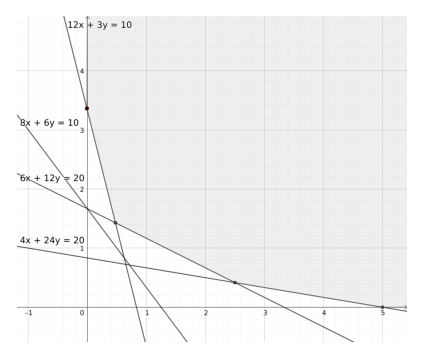
\includegraphics[width=190pt, height=190pt]{fig6.eps}
	\caption{Dopustiv region duala.}
	\label{fig:fig6-dual-region}
\end{figure}

Dualnost se najlakše opisuje kao odnos između problema maksimizacije i problema minimizacije, bez obzira koji od ta dva problema je primal, ($P$) a koji   dual ($D$). 
Kompletna lista mogućih odnosa između ograničenja
jednog problema i promjenljivih u drugom problemu je data sljedećom tabelom.
\begin{table}[!ht]
	\centering
	\begin{tabular}{l|l}
		($P$) & ($D$) \\ \hline
		ograničenja $\leq$  & promjenljive $\geq 0$ \\
		ograničenja $=$     & promjenljive (neograničene) \\
		ograničenja $\geq$  & promjenljive $\leq 0$ \\
		promjenljive $\geq 0$    & ograničenja $\geq$ \\
		promjenljive (neograničene) & ograničenja $=$ \\
		promjenljive $\leq 0$         & ograničenja $\leq$ \\ \hline
	\end{tabular}
	
	\caption{Odnos promjenljivih i ograničenja problema ($P$) i odgovarajućeg duala ($D$).}  \label{tab:primal-dual-relation}
\end{table}
\\
\textit{Napomena}. Simpleks metod ne garantuje   rješavanje proizvoljnog problema LP u polinomijalnom broju koraka u odnosu na veličinu ulaza (pogledati zadatak 6, u prethodnoj glavi). % V. Klee and G. Minty constructed an example LP: simplex method needs 2^n iterations to solve it 
%Dakle, iz njega se ne može zaključiti da je problem rješavanja generalnog LP problema   polinomijalno rješiv. 
Međutim, rješavanje problema LP-a je moguće u polinomijalnom vremenu, uz pomoć metoda \emph{unutrašnje tačke} (eng. interior point method), konstruisan od strane N. Karmakar-a sredinom 80ih godina prošlog vijeka. Radi kompleksnosti samog algoritma i njegovog izvođenja, mi ga ne prikazujemo u glavnom dijelu knjige, već u Apendiksu~\ref{appendix:interior_point} gdje čitalac kojeg interesuje ovaj metod može da vidi i prouči ideju i glavne korake konstrukcije ovog značajnog algoritma. 

\section{Farkašova lema}
Još jedna primjena teorije dualnosti LP-a se ogleda u dokazivanju Farkašove teoreme alternative. U suštini, njena geometirijska interpretacija kaže sljedeće: svaki vektor pripada ili datom zatvorenom konveksnom konusu (specijalan slučaj je ograničeni konveksni skup), ili postoji hiperravan koja razdvaja vektor od konusa; druge mogućnosti ne postoje. 

\begin{thm}
	Neka je $A\in \mathbb{R}^{m \times n}$ matrica i $c\in \mathbb{R}^n$. Onda jedan i samo jedan od  sljedeća dva sistema ima rješenje:
	\begin{enumerate}
		\item  $Ax \geq 0$  i $c^T x < 0$; \label{case:1}
		\item $A^T y = c$ i $y \geq 0$. \label{case:2}
	\end{enumerate}
\end{thm}

\begin{proof}
	Pogledajmo prvi sistem. Uočimo sličnosti sa   LP-om:
	\begin{align*}
		&\min c^T x \\
		&\mbox{t.d.} \\
		& A x \geq 0.
	\end{align*}
	Ako pogledamo desnu stranu ograničenja, vidimo da je vektor $x = 0$ 
	dopustivo rješenje problema, tako da problem ima barem jedno dopustivo rješenje. Zaključujemo da dati LP  ili ima optimalno rješenje ili je neograničen. Posmatrajmo njegov dual   dat sa 
	\begin{align*}
		&\max 0 \\
		&\mbox{t.d.} \\
		& A^T y  = c \\
		& y \geq 0.
	\end{align*}
	Primijetimo da, ako postoji barem jedno dopustivo rješenje za dati dual, optimalno rješenje je 0. Ako ne postoji niti jedno dopustivo rješenje, problem je nedopustiv. 
	
	Iz odnosa definisanog primala i njegovog duala zaključujemo:
	\begin{itemize}
		\item primal ima optimalno rješenje akko  dual ima optimalno rješenje; 
		\item primal je neograničen  akko je njegov dual nedopustiv.  
	\end{itemize}
	Odgovorimo sada na pitanje kada primal ima optimalno rješenje. Ono što vidimo je da ako bi $x$ bio dopustiv tako da je $c^Tx < 0$,  to bi onda i bilo koje $kx$, za proizvoljno $k>0$ bilo takođe dopustivo. Iz toga bi slijedilo da vrijednost funkcije cilja nije ograničena odozdo, tj. teži ka -$\infty$. Dakle, u tom slučaju je problem neograničen. Zaključujemo da, kad god  primal ima optimalno rješenje, ta vrijednost mora biti 0 i dostiže se za $x =0$. Inače, problem je neograničen. Dalje, ako primal ima optimalno rješenje, to  je ekvivalentno sa tim da je sistem iz slučaja  \ref{case:1} ove teoreme nedopustiv (nema rješenja).  Ako sistem iz slučaja  \ref{case:1}  ima rješenje, primal je neograničen (vrijedi i obrnut smjer). Ako pogledamo   dualni problem, dual ima optimalno rješenje akko sistem iz  slučaja  \ref{case:2}   ima rješenje. Slično, dual nije dopustiv akko je sistem iz  slučaja   \ref{case:2}  nedopustiv (nema rješenje). Iz niza prethodnih ekvivalencija, zaključujemo da vrijedi: 
	\begin{itemize}
		\item Sistem iz  slučaja  \ref{case:1}  nema rješenje akko sistem iz  slučaja  \ref{case:2}   ima rješenje. 
		\item Sistem iz  slučaja  \ref{case:1}  ima rješenje akko sistem iz  slučaja  \ref{case:2}  nema rješenje. 
	\end{itemize}
\end{proof}

\begin{primjer}
	Ovim primjerom analizirajmo geometrijsku interpretaciju Farkašove leme. Neka je dat sistem:
\end{primjer}

\begin{align*}
	& \underline{x_1 + 4 x_2  < 0: c^T x}\\  
	& 2 x_1 + 3 x_2 \geq 0 \\
	& 3 x_1 + 2 x_2 \geq 0 \\
	& 4 x_1 + x_2 \geq 0 \\
	& -x_1 + 3 x_2 \geq 0: Ax \geq 0.
\end{align*}

Pogledajmo kako izgleda sistem iz slučaja \ref{case:2}. Taj sistem je dat sa:
\begin{align*}
	&2 y_1 + 3 y_2 + 4 y_3 - y_4 = 1\\
	&3y_1 + 2 y_2 + y_3 + 3 y_4 = 4 \\
	& y_1, y_2, y_3, y_4 \geq 0. 
\end{align*}
\begin{figure}[!ht]
	\centering
	
\includegraphics[width=350pt, height=260pt]{farkas-geometry.eps}
	\vspace{-1cm}
	\caption{Geometrijska interpretacija Farkašove leme.}
	\label{fig:farkas-slika}
\end{figure}
Iz geometrijske interpretacije slijedi da se vektor $c =(1,4)^T$ može predstaviti kao linearna kombinacija vektora vrsta matrice $A$, kao što vidimo na Slici~\ref{fig:farkas-slika}. Vektor $c =(1,4)^T$ se nalazi unutar linearnog pokrivača $S^A = span\{a_1, \ldots, a_n \} = \{\sum_{i=1}^n \lambda_i a_i \mid \lambda_i \in \mathbb{R}\}$. što implicira da početni sistem nema rješenje. 
Kada bismo posmatrali $c=(5,0)^T$, zaključili bi da se on ne može izraziti kao linearna kombinacija vektora vrste matrice $A$, jer je van prostora  $S^A $. Prema tome, rješenje početnog problema za ovu konfiguraciju bi postojalo.  

%Furije–Mockin elimination ==> Problem dopustivosti...
\section{Furije–Mockinov metod eliminacije}
%https://faculty.math.illinois.edu/~mlavrov/docs/482-fall-2019/lecture19.pdf
Jedno od važnih pitanja vezano za problem  LP-a je sljedeće. 
\emph{Neka su date matrica $A \in \mathbb{R}^{m \times n}$ i vektor $b \in \mathbb{R}^m$, da li je skup $P = \{x \in \mathbb{R}^n \colon A x \leq b\}$ neprazan?} Dakle, da li postoji barem jedno dopustivo rješenje linearnog programa? 	

Problem dopustivosti može da služi i da odgovorimo na sljedeće pitanje: 
\emph{Da li je optimalna vrijednost funkcije cilja problema LP-a veća od neke unaprijed zadate  vrijednosti k?}
Na ovo pitanje možemo odgovoriti pomoću  \emph{Furije–Mockinovog} metoda eliminacije. Pored osnovne primjerne, ovaj algoritam može poslužiti za dokazivanje Farkašove leme. Jedna od praktičnih primjena  ove metode je u teoriji informacija, konkretno u informaciono-teorijskim dokazima ostvarivosti koji se opisuju uslovima pod kojima je zagarantovano postojanje šeme kodiranja sa dobrim performansama. Ovi uslovi se često opisuju linearnim sistemom nejednakosti, koji su upravo ulazne vrijednosti  \emph{Furije–Mockinove} eliminacije. 

Metoda  \emph{Furije–Mockinove} eliminacije strukturalno drugačija  od simpleks metode. Ideja algoritma je zasnovana na redukciji problema sa $n$ promjenljivih na ekvivalentan problem koji sadrži $n-1$ promjenljivih. Ekvivalentnost se posmatra u odnosu na svojstvo da početni problem ima rješenje akko ga ima i redukovani problem. Eliminacija promjenljivih se vrši iterativno, odnosno, u svakom koraku se redukuje broj promjenljivih za jedan. Na kraju se početni sistem svodi na sistem sa jednom promjenljivom, za koji se lako može provjeriti da li sadrži dopustivo rješenje.

Ponovimo, glavni korak ovog metoda je redukcija problema na ekvivalentan problem sa manjim brojem promjenljivih. Pretpostavimo da su ograničenja data sa promjenljivima $x_1,\ldots, x_n$ i da želimo da eliminišemo promjenljivu $x_n$. Za svako od ograničenja
\begin{equation}\label{eq:inequality_i}
	a_{i,1} x_1 + \cdots + a_{i,n} x_n \leq b_i
\end{equation}
vrijedi jedna od sljedećih alternativa 
\begin{itemize}
	\item  $x_n \geq \frac{b_i - a_{i,1}x_1- \cdots - a_{i, n-1} x_{n-1} }{a_{i,n}}=L_i$ ili 
	\item   $x_n \leq \frac{b_i - a_{i,1}x_1- \cdots - a_{i, n-1} x_{n-1} }{a_{i,n}}=U_i$
\end{itemize}
$i=1,\ldots, m$, zavisno od toga da li je $a_{i,n} >0$ ili $a_{i,n} <0$. U slučaju da je $a_{i,n} = 0$,  ostavljamo  ograničenje (\ref{eq:inequality_i}) nepromijenjeno, jer   $x_n$  ne učestvuje u datom ograničenju. Na ovaj način ćemo dobiti najviše $m$ gornjih i donjih granica za $x_n$ koje se mogu izraziti preko $n-1$ promjenljivih, tj. 
$$  x_n \geq L_1, \ldots, x_n\geq L_k \mbox{ te }  x_n \leq U_1, \ldots, x_n \leq U_l,$$
za neke $k,l \in \mathbb{N}$, $k+l \leq m$.
Moguće je izabrati $x_n$ koje zadovoljava gornja ograničenja akko 
\begin{equation}\label{eq:min_max_xi}
	\max\{L_1,\ldots, L_k \} \leq x_n \leq \min \{ U_1, \ldots, U_l \},
\end{equation}
%https://faculty.math.illinois.edu/~mlavrov/docs/482-fall-2019/lecture19.pdf
jer bi tada postojalo nešto između najveće donje granice i najmanje gornje granice za vrijednost promjenljive $x_n$. Međutim, kako su sve donje i gornje granice izražene preko nepoznatih promjenljivih $x_1, \ldots, x_{n-1}$, ne može se ustanoviti koje od njih su veće, a koje manje. Kompromis postižemo dodavanjem  sljedećih nejednakosti 
$$\begin{array}{cccc}
	L_1 \leq U_1 & L_1 \leq U_2   &  \cdots   & L_1 \leq U_l \\
	L_2 \leq U_1 & L_2  \leq U_2  &  \cdots   & L_2 \leq U_l \\
	\vdots       &     \vdots     &   \ddots  & \vdots       \\
	L_k \leq U_1 &  L_k \leq U_2  &   \cdots  & L_k \leq U_l \\
\end{array}$$ 
Ako postoji neka vrijednost  $x_n$ koja zadovoljava sva ograničenja (\ref{eq:min_max_xi}), onda je za sve $i,j$, 
$L_i \leq x_n \leq U_j$. Obrnuto, ako svih $k \cdot l$ nejednakosti vrijede, onda vrijedi i (\ref{eq:min_max_xi}), pa se može izabrati neki $x_n$ između $\max$ i $\min$ gornje granice. 

Prema tome, početni problem je redukovan na sistem od $n-1$ promjenljivih sa dodatnih  $k \cdot l$ nejednakosti izraženih gore, uz originalna ograničenja koja ne uključuju $x_n$. Ovaj proces nastavimo iterativno, dok ne dobijemo samo jednu promjenjivu sa dodatnim ograničenjima  i potom (trivijalno) riješimo sistem. 

\begin{primjer} Pretpostavimo da nam je dat sistem nejednačina:
\end{primjer}
\begin{align*}
	&x - y \leq 1 \\
	&-x + 2y \geq 1 \\
	& 3x - 5y \geq 1 \\
	& x,y \geq 0.
\end{align*}
Eliminišimo promjenljivu $y$ iz sistema. Kako je $x-y \geq 1 \Rightarrow y \leq x -1 $, 
$-x + 2y \geq 1 \Rightarrow y \geq \frac{x+1}{2}$, te $ 3x - 5y \geq 1 \Rightarrow y \leq \frac{3x-1}{5}$, uparivanjem gornjih i donjih granica dobijamo
$$
\begin{cases}
	&\frac{x+1}{2} \leq x-1 \\
	& 0 \leq x-1 \\
	& \frac{x+1}{2} \leq \frac{3x-1}{5} \\
	& 0 \leq \frac{3x-1}{5} \\
	& x \geq 0, y \geq 0.  	
\end{cases}
$$
Ove nejednakosti se mogu pojednostaviti u donje i gornje granice za $x$, na sljedeći način:
$$
\begin{cases}
	&x \geq 3 \\
	& x \geq 1 \\
	& x \geq 7 \\
	& x \geq \frac{1}{3} \\
	& x \geq 0.	
\end{cases}
$$
Sve ove nejednakosti su donje granice. Vidimo da vrijednost $x=7$ zadovoljava sve navedene nejednakosti.
Tada, donje i gornje granice za $y$ postaju uslovi: $y \leq 6, y \geq 4, y \leq 4$ te $y \geq 0$. Prema tome, možemo uzeti vrijednost $y=4$, čime smo pronašli i dopustivo rješenje polaznog sistema. 
%kompleksnost i Farkasova lema...
%  dualna simpleks metoda ? https://www.youtube.com/watch?v=lyNHVnT9zVk&list=PLY9yf2-4yyeT0Jh80w5yuevm0o9lAAUJg&index=40
\vspace{1.5cm}
\section{Zadaci}
\begin{enumerate}
	\item %http://www.nitjsr.ac.in/course_assignment/CA02CA3103%20RMTLPP:%20Duality.pdf
	Napišite odgovarajući dual linearnog programa:
	\begin{align*}
		&\max x_1 - x_2 + 3 x_3 \\
		& \mbox{t.d.} \\
		& x_1 + x_2 + x_3 \leq 10 \\
		& 2x_1 - x_2 - x_3 \leq 2 \\
		& 2x_1 - 2x_2 - 3 x_3 \leq 6 \\
		& x_1, x_2, x_3 \geq 0.
	\end{align*}
	\item    	Napišite odgovarajući dual linearnog programa:
	\begin{align*}
		&\min 3 x_1 - 2 x_2 + 4 x_3 \\
		& \mbox{t.d.} \\
		& 3x_1 + 5 x_2 + 4 x_3 \geq 7 \\
		& 6 x_1 + x_2 + 3 x_3 \geq 4 \\
		& 7 x_1 - 2 x_2 - x_3 \leq 10 \\
		& x_1 - 2 x_2 + 5 x_3 \geq 3 \\
		& 4 x_1 + 7 x_2 - 2 x_3 \geq 2 \\
		& x_1, x_2, x_3 \geq 0.
	\end{align*}
	\item Napišite dual sljedećeg linearnog programa:
	\begin{align*}
		&\min x_1 - 3 x_2 - 2 x_3 \\
		&\mbox{t.d.} \\
		& 3 x_1 - x_2 + 2 x_3 \leq 7 \\
		& 2 x_1 - 4 x_2 \geq 12 \\
		& -4x_1 + 3x_2 + 8 x_3 = 10 \\
		& x_1, x_2\geq 0 \\
		& x_3 \in \mathbb{R}. 
	\end{align*}
	\item %http://www.nitjsr.ac.in/course_assignment/CA02CA3103%20RMTLPP:%20Duality.pdf
	Pokazati da je dual dualnog problema ponovo primalni problem ($P$).
	
	\item Vratite se na Primjer~\ref{primjer:dual}. Vrijednost 210 u drugom ograničenju primarnog problema  ($P$)  zamijenite sa 420 i diskutujte optimalna rješenja  ($P$)  i  ($D$)  na sličan način kako je urađeno  u samom primjeru.
	
	\item Ako je primalni problem ($P$) neograničen (ima neograničenu funkciju cilja), njegov dual nije dopustiv. Dokazati.
	\item Pokazati da vrijede odnosi dati u Tabeli~\ref{tab:primal-dual-relation}.
	\item Istražiti verziju simpleks metoda zvanu \emph{Dualni simpleks metod}.
	\item Koristeći Farkaš-ovu lemu, pokazati sljedeći rezultat. 
	
	Tačno jedan od sljedećih sistema ima rješenje:%https://web.stanford.edu/class/msande310/hw2sol.pdf
	\begin{enumerate}
		\item $Ax > 0$; 
		\item $y^T A = 0, y \geq 0, y \neq 0.$
	\end{enumerate}
	\item Koristeći Farkaš-ovu lemu, pokazati sljedeći rezultat. 	Tačno jedan od sljedećih sistema ima rješenje:%https://web.stanford.edu/class/msande310/hw2sol.pdf
	\begin{enumerate}
		\item $Ax \leq b$; 
		\item $y^T A = 0, y^T b < 0, y \geq 0.$
	\end{enumerate}
	\item  %https://www.cs.cmu.edu/~odonnell/toolkit13/lecture13-anonymous.pdf
	Koristeći Furije-Mockin-ov metod eliminacije, pokazati da postoji rješenje za sljedeći sistem nejednačina:
	\begin{align*} 
		&x - 5y + 2 z \geq 7 \\
		&3x - 2y - 6 z \geq -12 \\
		& -2x + 5y - 4z \geq -10 \\
		& -3x + 6y - 3z \geq -9 \\
		& -10 y + z \geq -15 \\  
		& x,y,z \geq 0.
	\end{align*}
	\item Pomoću Furije-Mockin-ovog metoda eliminacije, pokazati da je sistem 
	\begin{align*}
		&x_1 \geq 0 \\
		&x_2 \geq 0 \\
		& x_1 + x_2 \leq -2 
	\end{align*}
	nedopustiv.%https://people.inf.ethz.ch/fukudak/lect/opt2011/aopt11note4.pdf
	
	\item Neka su $x^0$ i $y^0$ dopustive tačke za polazni (kanonski) LP i njegov dual. Dokazati da su te dvije tačke optimalne ako i samo ako važi 
	
	$$\langle Ax^0-b,y^0\rangle=\langle A^Ty^0-c,x^0\rangle=0$$
	
	\item Formirati dualan LP za problem
 
	 \begin{align}
		&\min  -x_1+2x_2+3x_3\nonumber \\
		&\mbox{t.d.} \nonumber \\
		 & x_1-x_2+2x_3=1\nonumber\\
		 & 2x_1+x_2\leqslant 3\nonumber \\
		 & x \geq 0\nonumber \\
		 & x_1\leqslant 0,\ x_2\geqslant 0, x_3\geqslant 0 \nonumber
	\end{align}
	pa riješiti oba problema.
	
	\item Koristeći teoriju dualnosti, riješiti problem linearnog programiranja
	
	\begin{align}
		&\min\  x_1+2x_2+\cdots +nx_n\nonumber\\
			&\mbox{t.d.}\nonumber\\
		& x_1\geqslant 1\nonumber\\
		& x_1+x_2\geqslant 2 \nonumber\\
		& \vdots\nonumber\\
		& x_1+x_2+\cdots+x_n\geqslant n\nonumber\\
		&x_1\geqslant 0,\ x_2\geqslant 0,\ldots,x_n\geqslant 0.
	\end{align}
\end{enumerate}
%\newpage
\chapter{Cjelobrojno linearno programiranje}\label{chp:ilp}

%https://www.google.com/url?sa=t&source=web&rct=j&url=https://web.mit.edu/15.053/www/AMP-Chapter-09.pdf&ved=2ahUKEwiN0cef_f7xAhU0CRAIHWLqCw0QFjAfegQILBAC&usg=AOvVaw1cQCbZJQbc55Z0VLPue2ul
U mnogim realnim problemima, promjenljive odluke ne dobijaju neprekidne, već isključivo diskretne vrijednosti. Npr. kod problema dodjele poslova određenim mašinama, zahtijevaju se promjenljive koje su diskretnog tipa, kojima se definiše koji posao će biti dodijeljen kojoj mašini. U slučaju da su u nekom modelu sve promjenljive odluke cjelobrojne, tada kažemo da je riječ o problemu \emph{cjelobrojnog programiranja} (eng. \emph{integer programming}). 
U ovoj glavi ćemo analizirati koncepte   \emph{cjelobrojnog linearnog programiranja} (ILP), gdje se, pored integralnosti (cjelobrojnosti) promjenljivih, zahtijeva da funkcija cilja  i sva ograničenja u modelu budu linearni izrazi po promjenljivima. Prema tome, ILP ima opšti oblik:
\begin{align}
	& \max c^T x \nonumber\\
	& t.d. \nonumber \\
	& A x \leq b \nonumber \\
	& x \geq 0 \nonumber\\
	& x_i \in \mathbb{Z}, \forall i. \label{ilp-formulation}
\end{align}

Problemi cjelobrojnog linearnog programiranja se veoma često sreću i u teoriji i u praksi, te je, samim tim, važno poznavati i tehnike rješavanje ovih problema. Sa druge strane, pokazuje se da je rješavanje ovih problema u velikom broju slučajeva značajno teže nego rješavanje klasičnih problema linearnog programiranja. U narednom odjeljku ćemo modelovati nekoliko poznatih optimizationih problema pomoću koncepta cjelobrojnog linearnog programiranja. U Odjeljku~\ref{sec:transformILP} ćemo prikazati neke korisne tehnike transformacije nekih nelinearnih izraza u IP kako bi se dobio ekvivalentan ILP model. U Odjeljku~\ref{sec:kompleksnostILP} ćemo pokazati da je rješavanje ILP-a NP težak problem. Tehnike rješavanja ILP-a ćemo detaljnije razmatrati u Glavi~\ref{chap:rjesavanjeILP}.
\section{Modelovanje nekih problema cjelobrojnog linearnog programiranja}


\begin{primjer}
	\emph{Cjelobrojni problem jednodimenzionalnog ruksaka.} Neka je dato $n$ proizvoda i neka je težina $i$-tog proizvoda jednaka $w_i$, dok je vrijednost $i$-tog proizvoda jednaka $c_i$, $i=1,\ldots,n$. Koje od proizvoda treba da stavimo u ruksa, čija je maksimalna težina (kapacitet) $C>0$, tako da   vrijednost proizvoda u ruksaku bude maksimalna, poštujući  kapacitet  ruksaka? 
	
	\emph{Rješenje}. Definišimo promjenljive $x_i$, koje dobijaju vrijednost 1 ako  $i$-ti proizvod uključujemo u ruksak, odnosno, vrijednost 0, ako $i$-ti proizvod nije uključen u ruksak, za $i=1,\ldots,n$. Ograničenje kapaciteta ruksaka se modeluje sa $\sum_{i=1}^n w_i x_i \leq C$. Funkcija cilja maksimizuje ukupnu vrijednost odabranih proizvoda i modeluje se uz pomoć linearne kombinacije $f(x) = \sum_{i=1}^n c_i x_i$. 
\end{primjer}
\begin{primjer}
	\emph{Jedan problem rasporeda radnika u dežurstvu}. Uprava bolnice želi da napravi raspored dežurstva po sedmičnim noćnim smjenama za svoje medicinske sestre.  Potrebno je da broj medicinskih sestara u noćnoj smjeni za $j$--ti dan bude barem (cio broj) $d_j, j = 1,\ldots 7$. Svaka
	medicinska sestra radi pet dana zaredom u noćnoj smjeni. 
	
	\emph{Pronaći minimalan broj medicinskih sestara koje bolnica treba da zaposli, da bi se takve smjene mogle organizovati.}
	
	\emph{Rješenje}. Označimo sa $x_i$ broj medicinskih sestara koje svoju noćnu smjenu započinju na $i$-ti dan. Potrebno je minimizovati funkciju 
	$f = \sum_{i=1}^7 x_i$ pod uslovima da su ispunjeni zahtjevi za brojem medicinskih sestara, što je modelovano sa:
	\begin{itemize}
		\item $x_1 + x_2 + x_3 + x_4 + x_5 \geq d_5 $
		\item $x_2 + x_3 + x_4 + x_5 + x_6 \geq d_6$
		\item $x_3 + x_4 + x_5 + x_6 + x_7 \geq d_7$
		\item $x_4 + x_5 + x_6 + x_7 + x_1 \geq d_1 $
		\item $x_5 + x_6 + x_7 + x_1 + x_2   \geq d_2$
		\item $x_6 + x_7 + x_1 + x_2 + x_3  \geq d_3$
		\item $  x_7 + x_1 + x_2 + x_3 + x_4 \geq d_4$
	\end{itemize}
	uz nenegativne uslove 
	\begin{itemize}
		\item $x_i \geq 0, x_i \in \mathbb{Z}$, $j=1,\ldots,7.$
	\end{itemize}
	Primijetimo da su u ovom problemu promjenljive  cjelobrojne. Primijetimo da sve varijable figurišu u tačno pet ograničenja, što odgovara uslovu da svaka od sestara radi pet dana zaredom u noćnoj smjeni.
	%Ovaj model pripada paradigmi cjelobrojnog linearnog programiranja.
\end{primjer}
\begin{primjer}
	\emph{Problem oglašavanja}. Kompanija želi da se oglašava u medijima. Postoji nekoliko načina oglašavanja:  televizijsko, novinsko i radio oglašavanje. Cijena svakog medija sa pokrivenošću publike navedena je u Tabeli~\ref{tab:tab_model_advertising}.
	
	\begin{table}[!ht]
		\centering
		\begin{tabular}{l|c|c|c} \hline
			\                  & Televizija & Novine & Radio  \\ \hline
			Cijena po oglašavanju      & 2000       & 600    & 300    \\
			Broj gledalaca/slušalaca/čitalaca      & 10000      & 4000  & 1800 \\ \hline
		\end{tabular}
		\caption{Cijene reklama sa brojem gledalaca/slušalaca/čitalaca.}
		\label{tab:tab_model_advertising}
	\end{table}
	
	
	Novine ograničavaju broj oglasa za kompanije na deset (po sedmici). Štaviše, kako bi se uravnotežilo oglašavanje između sve tri vrste medija, na radiju se ne smije pojaviti više od polovine ukupnog broja oglasa za kompaniju. Najmanje 10\% od svih oglasa bi se trebalo pojaviti na televiziji. Sedmični budžet za oglašavanje date kompanije iznosi 18200KM. 
	
	\emph{Koliko oglasa treba zakupiti za svaku od tri vrste medija sa ciljem povećanja ukupnog broja gledalaca?}
	
	\emph{Rješenje}.   Označimo sa $x_1$ broj oglasa na televiziji, sa $x_2$ broj oglasa u novinama i $x_3$ broj oglasa na radiju. Potrebno je maksimizovati   uspješnost oglašavanja, tj. funkciju 
	$f(x) = 10000 x_1 + 4000 x_2 + 18000 x_3.$ Uslovi pod kojima tražimo rješenja su modelovani na sljedeći način:
	\begin{itemize}
		\item $2000 x_1 + 600 x_2 + 300 x_3 \leq 18200$ (uslov za cijenu);
		\item  $ x_2 \leq 10$ (limit na broj reklama u novinama);
		\item $x_1 + x_2 \geq x_3$ (uslov za maksimalno polovinu oglašavanja na radiju);
		\item ${x_1}\geq 0.1\cdot (x_1 + x_2 + x_3)$ (uslov za broj reklama na televiziji);
		\item $x_i \geq 0, x_i \in \mathbb{Z}, i=1,2,3$.
	\end{itemize}
	
	%U ovom problemu možemo još   primijetiti da u funkciji cilja   
	%nisu korišteni egzaktni koeficijenti (za broj gledalaca) već brojevi koji su proporcionalni nekoj vrijednosti (1000). Takve transformacije su invarijantne i ne utiču na potragu za optimalnim rješenjem  problema, a doprinose većoj čitljivosti modela.
\end{primjer}
\begin{primjer}
	
  	%https://www.math.unipd.it/~luigi/courses/metmodoc1819/m01.modelli.00.en.pdf
	\emph{Problem pokrivanja}. Telefonska kompanija želi da instalira antene na neka mjesta kako bi pokrila šest oblasti. Postoji pet mogućih mjesta za instaliranje antena. Nakon urađenih simulacija, za svaku oblast utvrđen je intenzitet signala koji antena šalje, kad je postavljena na određenom mjestu. Tabela~\ref{tab:tb-3} daje   primjer jedne instance problema sa nivoima intenziteta signala.
	
	\begin{table}[!ht]
		\centering
		\begin{tabular}{c|cccccc} \hline
			\              & oblast1 & oblast 2 & oblast 3 & oblast 4 & oblast 5 & oblast 6 \\ \hline
			Mjesto $A$     & 10  & 20 & 16 & 25 & 0   & 10   \\
			Mjesto $B$     & 0   & 12 & 18 &  23 & 11 & 6   \\
			Mjesto $C$     & 21  &  8 & 5  &  6 & 23  &  19 \\
			Mjesto $D$    &  16 &  15 & 15 &  8 & 14 & 18   \\
			Mjesto $E $    &  21 & 13 & 13 & 17 & 18  & 22    \\ \hline
		\end{tabular}
		\caption{Intenziteti signala.}
		\label{tab:tb-3}
	\end{table}
	
	Prijemnici prepoznaju samo signale čija je jačina najmanje   $d>0$. Nadalje, ne može da se desi da više od jednog signala  dostiže jačinu signala $d$ u istoj oblasti, inače bi to prouzrokovalo smetnje u prijemu. %Na kraju, antena se može postaviti na mjesto $E$ samo ako je antena instalirana i na mjestu $D$ (ova antena bi služila kao most). 
	
	\emph{Potrebno je odrediti gdje treba postaviti antene kako bi se signalom pokrio maksimalan broj oblasti.}
\end{primjer}
%https://www.math.unipd.it/~luigi/courses/metmodoc1920/m01.modelli.00.en.beamer.pdf
\emph{Rješenje}. Posmatrajmo ovaj problem malo opštije i definišimo: 
\begin{itemize}
	\item $I$: skup mijesta;
	\item $J$: skup oblasti;
	\item $\sigma_{ij}$ : indikator nivoa signala antene   smještene u mjestu $i \in I$ u oblasti $j \in J$;
	\item $d$: parametar koji označava minimalnu jačinu signala;
	\item $N$: parametar koji označava maksimalni broj signala iznad granice koju prijemnik u jednoj oblasti može da prepozna (u našoj instanci imamo da je $N=1$);
	\item $x_i$: binarna promjenljiva koja uzima vrijednost 1 ako je antena smještena u mjestu $i\in I$, 0 inače;
	\item  $z_j$ : binarna promjenljiva koja uzima vrijednost 1 ako je oblast $j \in J$ pokrivena signalom, 0 inače;
	\item $M_j$: dovoljno veliki parametar, npr. za svako mjesto $j \in J$, $M_j= |\{ i \in I \mid \sigma_{ij} \geq d\}|$. Primijetimo da $M_j$ označava gornje ograničenje za broj mijesta iz kojih se dovoljno jak signal može poslati predajniku u oblasti $j\in J$. 
\end{itemize}
Formulišimo sada (cjelobrojni) linearni program ovog problema. 
Funkcija cilja je data sa:
$$ f(x) = \min \sum_{j \in J} z_j $$
tako da
\begin{align}
	& \sum_{\{i \in I \mid \sigma_{ij} \geq d \}} x_i \geq z_j, \forall j \in J \label{const:ob-1}\\
	&\sum_{\{i \in I \mid \sigma_{ij} \geq d \}} x_i  \leq N + M_j( 1 - z_j), \forall j \in J \label{const:bound-2} \\ 
	& x_i, z_j \in\{0, 1\}, \forall i \in I, \forall j \in J   \label{const:vars-3}
\end{align}

Ograničenje (\ref{const:ob-1}) zahtijeva da, ukoliko je oblast pokrivena signalom, tj. ako je $z_j = 1$, tada mora postojati neko mjesto $i \in I$ koji ima antenu jačine barem $d$ koja pokriva tu oblast. U slučaju da je $z_j=0$, ovo ograničenje je redundantno. 

Ograničenje~(\ref{const:bound-2}) ograničava maksimalan broj signala koje prijemnici u oblasti $j\in J$ mogu obraditi. Preciznije, ako je oblast $j\in J$ pokrivena, tj. $z_j=1$, onda  predajnikom u oblasti $j \in J$ ne može da bude prihvaćeno više od $N$ (dovoljno jakih) signala. U slučaju da je $z_j = 0$, ovo ograničenje postaje redundantno, jer je ova oblast isključena iz rješenja, zbog čega i ukupan broj signala koji se šalje predajniku nije relevantan. Treba napomenuti da je ovo takozvano \emph{big-M} ograničenje, koje ćemo analizirati u narednim sekcijama.

Ograničenjima (\ref{const:vars-3}) definisana je binarna priroda promjenljivih. 

%\printbibliography[heading=subbibliography,notkeyword=this]
\begin{primjer}
	\emph{Jedan lokacijski problem}. Lokacijski problemi se često postavljaju na sljedeći način: pretpostavimo da postoji $n$ postrojenja (prodavnica)  i  $m$ kupaca. Dva pitanja koja treba da budu obuhvaćena rješenjem su:
	\begin{enumerate}
		\item koja od $n$ postrojenja otvoriti i
		\item koje  postrojenje koristiti za opsluživanje pojedinih kupaca, kako bi se zadovoljila fiksna potražnja svakog od kupaca uz minimalni trošak otvaranja postrojenja.
	\end{enumerate}
	Prije nego što modelujemo ovaj problem, uvedimo sljedeću notaciju.
	\begin{itemize}
		\item  $f_{i}$: označava (fiksni) trošak otvaranja postrojenja $i$, za  $ i = 1,  \ldots, n$;
		\item $c_{ij}$: označava troškove zadovoljenja potražnje  kupca $j$ od strane postrojenja $i$ (cijena dostave, cijena proizvoda,  itd.), $i = 1, \ldots, n$, $j = 1,  \ldots, m$;
		\item $d_{j}$: označava ukupnu potražnju kupca $j$, $j = 1, \ldots, m$;
		\item $u_{i}$: označava maksimalnu količinu proizvoda (kapacitet zadovoljenja) koji se mogu nabaviti u postrojenju $i$, tj. $u_{i}$ je kapacitet postrojenja $i$.
	\end{itemize}
	Definišimo sljedeće promjenljive odlučivanja:
	
	\begin{itemize}
		\item $x_i \in \{0,1\}$, gdje je $x_i = 1$ ako je postrojenje $i$ otvoreno, a inače 0.
		\item $y_{ij} \in \mathbb{R}^+$  označava dio ukupne potražnje $d_j$ kupca $j$ koja je ispunjena u prodavnici $i$.  
	\end{itemize}
	
	\emph{Rješenje}. Funkcija cilja problema je data sa:
	\begin{align}
		\min f = \sum_{i=1}^n f_i x_i  + \sum_{i,j} c_{ij} y_{ij} d_j, \label{const:location-objective}
	\end{align}
	pod uslovima
	
	\begin{align}
		&\sum_{i} y_{ij} = 1, \forall j\in\{1,\ldots,m\}\label{const:location-1} \\
		&~\sum_{j} d_j y_{ij} \leq u_i x_i, \forall i \in \{1,\ldots,n\}\label{const:location-2}.
	\end{align}
	
	Funkcija cilja (\ref{const:location-objective}) minimizuje ukupnu cijenu zadovojenja  (dijela) potreba kupaca u postrojenjima i cijene otvaranja postrojenja. 
	
	Ograničenje (\ref{const:location-1}) garantuje da su potrebe svakog kupca zadovoljene.  
	Ograničenje (\ref{const:location-2}) ograničava da, ukoliko je postrojenje $i$ otvoreno, ono može da ponudi kupcima onoliko koliko mu njegov kapacitet dozvoljava.  
	
	
	Ovaj model pripada modelu \emph{mješovitnog linearnog programiranja}, gdje u istom modelu postoje i cjelobrojne i neprekidne promjenljive.
\end{primjer}

Sljedeći primjer spada u modele \emph{binarnog linearnog programiranja}. 

\begin{primjer}
	
	\emph{Problem postrojenja sa neograničenim kapacitetom.}
	Čest slučaj je varijacija prethodnog problema lokacija gdje je $ u_{i} = + \infty,i=1\ldots,m$. U ovom slučaju optimalna strategija se sastoji u zadovoljenju kompletne (neparcijalne) potražnje kupca $j$ iz najbližeg otvorenog objekta. Zbog toga, neprekidne promjenljive  $y_{ij}$ možemo zamijeniti binarnim promjenljivima $z_{ij}$, $i=1,\ldots,n, j=1,\ldots,m$ pri čemu promjenljiva dobija vrijednost 1 ako je kupac $j$ snabdjeven od strane postrojenja $i$. Prema tome, model izgleda ovako:
	
	\begin{align*}
		&\min \sum_{i=1}^n f_i x_i  + \sum_{i,j} c_{ij} z_{ij} d_j \\
		& \mbox{t.d.} \nonumber \\
		& \sum_{i} z_{ij} = 1, \forall j\in\{1,\ldots,m\} \\
		& \sum_{j} d_j z_{ij} \leq M x_i, \forall i \in \{1,\ldots,n\} \\
		& x_i, z_{ij} \in \{0,1\} \mbox{ za } i = 1, \ldots, n, j = 1,  \ldots, m.
	\end{align*}
	Vrijednost $M>0$ je konstanta koja uzima neku veliku vrijednost (npr. zbir količine potražnji svih kupaca). Međutim, u praksi se često  izbjegava upotreba $M$-konstante, te se tako 
	ovo ograničenje mijenja sa $ z_{ij} \leq x_i$ 
	za $ i = 1, \ldots, n, j = 1,  \ldots, m$. % Ovakav pristup osigurava bolje performanse, jer se generišu preciznije linearne relaksacije o kojima će biti riječi u narednim sekcijama.
\end{primjer}
\begin{primjer}
	\emph{Problem rasporeda} (eng. scheduling problems). Čitava klasa problema koja se naziva sekvenciranje, raspoređivanje i usmjeravanje u osnovi su predstavljeni modelima cjelobrojnog programiranja. U ove probleme, na primjer, spadaju problemi rasporeda časova ili rasporeda ispita na fakultetima. Kod ovih problema postoje ograničenja u pogledu broja i kapaciteta učionica dostupnih u bilo kom trenutku, dostupnosti predavača na fakultetu u određeno vrijeme i preferencijama studenata ili nastavnika za određene rasporede. Kriterijumi za određivanje funkcije cilja mogu da budu različiti. Kod rasporeda polaganja ispita, može se minimizovati broj potrebnih termina za održavanje ispita, uz osnovni uslov da dva ispita moraju biti u različitim terminima ako postoji barem jedan student koji planira da polaže oba ispita.  Kod jednog problema rasporeda časova, raspoređivanje studenata u  učionice se može vršiti na  način da se minimizuje broj učenika koji ne mogu pohađati nastavu iz predmeta koji je njihov prvi izbor, u odnosu na ostale izbore.
	U tom slučaju, jasno je da imamo promjenljivu $X_{i,j,n}$ za   $i$-tog učenika 
	koji pohađa $j$-to predavanje tokom $n$-tog vremenskog perioda (recimo, vr	ijeme je diskretizovano po 45 min/čas) -- koja je jednaka 1 ako se student uklapa u takav raspored, inače 0. 
\end{primjer}
Posmatrajmo, ipak, malo specifičniji problem u odnosu na najopštiji, koji je dosta težak i za modelovanje, a kamoli za rješavanje. 
Razmotrimo raspoređivanje osoblja zaduženog za upravljanje letom aviona. 
Avionska kompanija treba da rasporedi svoje osoblje na rutama koje pokrivaju letove. Treba paziti, na primjer, da jedna posada treba da upravlja letom iz  Beograda u Zagreb (u 10:00), a zatim letom iz Zagreba u Cirih (u 14:00). Dakle, jedna posada bi trebalo da je uključena u rutu na kojoj upravlja različitim letovima. Prema tome, raspoređivanje posade na rutu $j$ se modeluje uz pomoć binarne promjenljive 
$$x_j = \begin{cases}
	1,& \mbox{ ako je barem jedna posada pridružena ruti } j \\
	0,& \mbox{ inače}. 
\end{cases}
$$
Dalje, definišimo 
$$a_{ij}= \begin{cases}
	1,& \mbox{ ako je let } i \mbox{ pridružen ruti } j \\
	0,& \mbox{ inače}.
\end{cases}
$$
Neka je $c_j$ cijena zaduživanja neke posade ruti $j$. Ovdje $a_{ij}$ definišu prihvatljive kombinacije letova sa rutama, uzimajući u obzir  karakteristike kao što su redoslijed krakova za uspostavljanje veza između letova sa uključenim vremenom  održavanja letova (iskrcavanje, istovar  kofera, utovar   novih kofera, ukrcavanje itd.) na istoj ruti leta posade.   

Model ovakvog problema je dat sa 
\begin{align}
	&\min \sum_{j=1}^n c_j x_j \nonumber\\
	&\mbox{t.d.} \nonumber \\
	& \sum_{j=1}^n a_{ij} x_j \geq 1, \forall i \in \{1,\ldots, n\} \label{ineq:set_cover} \\
	%&   a_{ij} \geq  x_j, \forall j \in \{1,\ldots, m\}  \\
	& x_i \in \{0, 1 \}, \forall i \in \{1, \ldots, n\} \\
	& a_{ij} \in \{0, 1\}, \forall i \in \{1, \ldots, n\}, j \in\{1,\ldots, m\} \nonumber
\end{align}

Ograničenje (\ref{ineq:set_cover}) nam govori da, za svaki let $i$, mora postojati barem jedna ruta $j$ za koju je barem jedna posada zadužena. Svakako,  više letova može da bude pridruženo jednoj ruti, pa je otuda suma na lijevoj strani veća ili jednaka 1. 
%Ograničenje (\ref{ineq:set_cover}) je poznato ograničenje koje se javlja u problemu pokrivanju  skupa (eng. \emph{set covering problem}).
\begin{primjer}
	\emph{Problem trgovačkog putnika} (eng.  {Traveling Salesman Problem -- TSP)}. Neka je dato $n$ gradova. Krenuvši od svog mjesta, putnik želi da posjeti ostalih $n-1$ gradova pod minimalnim troškovima i da se na kraju vrati u početni grad. U suštini, ovo je problem grafovske prirode, gdje je ulaz (bez smanjenja opštosti) kompletan težinski graf, a potrebno je naći Hamiltonovu konturu minimalne težine u datom grafu. Pod težinom konture se podrazumijeva zbir težina njenih grana. 
\end{primjer}
\emph{Rješenje}. Označimo težinu grane od grada $i$ do grada $j$ sa $c_{ij}$.  Definišimo (binarne) promjenljive 
$$x_{ij} = \begin{cases}
	1, \mbox{ ako putnik u svojoj ruti iz grada } i \mbox{ posjeti grad } j \\
	0, \mbox{ inače}. 
\end{cases}$$ 
Potrebno je nametnuti sljedeća ograničenja -- svaki grad se treba naći u ruti,  što možemo postići sa 
$$  \sum_{i=1}^n x_{ij} = 1, \forall j =1,\ldots, n,$$ 
što znači da se iz tačno jednog grada dolazi u svaki grad $j$, dok sličnim jednakostima nametnemo da se iz grada $j$ odlazi u tačno jedan drugi grad sa:

$$  \sum_{j=1}^n x_{ij} = 1, \forall i =1,\ldots, n$$ 
uz uslove $x_{ij}\geq 0$. Primijetimo sljedeće, ovakvi uslovi ne sprečavaju pojavu rješenja koja predstavljaju uniju disjunktnih podruta, što nije dopustivo rješenje za TSP. Ako pretpostavimo da je rješenje dato u obliku podruta $R_1, \ldots, R_k$, gdje je $R_i = \{ v_{i_1}, \ldots, v_{i_{p_i}} \}$, onda se pojava podruta  može izbjeći  dodavanjem dodatnih ograničenja u početni model problema. Tako problem sukcesivno rješavamo dodavanjem ograničenja, sve dok ne dobijemo rješenje koje je u stvari jedna ruta koja obuhvata sve gradove. Recimo, eliminacija pojave podrute $R_2$ (u odnosu na podrutu $R_1$) se vrši dodavanjem ograničenja
$$ \sum_{l=1}^{ {p_1}}\sum_{t=1}^{ {p_2}} x_{1_l, 2_t} \geq 1.$$
U najgorem slučaju, potrebno je dodati $2^n-1$ ovakvih ograničenja prije nego se dobije dopustivo rješenje. 
Generalno ograničenje koje služi za eliminaciju podruta u modelu TSP-a se može dodati sa:
\begin{align}
	\sum_{i \in S} \sum_{j \notin S} x_{ij} \geq 2, \forall S \subset [n].
\end{align}
%Postoje i druga ograničenja koja mogu da se dodaju za eliminaciju podruta, bez gore pomenutog iterativnog procesa, ali o njima će biti riječi u narednim sekcijama. 

\section{Tehnike transformacija nekih nelinearnih izraza u ILP-u}\label{sec:transformILP}

U prethodnom odjeljku je objašnjeno modelovanje nekih problema pomoću cjelobrojnog linearnog programiranja. Kao što se može vidjeti, modeli nekih problema pravolinijski slijede iz definicije samog problema, dok je za modelovanje nekih drugih, kompleksnijih problema, potrebno uključiti veći broj dodatnih promjenljivih i ograničenja. U ovom odjeljku ćemo prikazati neke standardne transformacije i tehnike, kojima različite (nelinearne) izraze transformišemo i modelujemo ih pomoću cjelobrojnih promjenljivih i linearnih ograničenja.
%\emph{Binarne promjenljive.} 



\subsection{Prepoznavanje binarnih promjenljivih}
Pretpostavimo da je potrebno uključiti sljedeće aktivnosti: (1) izgraditi novo postrojenje ili
(2) pokrenuti reklamnu kampanju ili (3) razviti novi proizvod. Jasno je da su u pitanju logičke odluke, odnosno odluke tipa ,,da ili ne'', pa ih, prema tome, modelujemo   uvođenjem  binarnih promjenljivih $x_i \in \{0, 1 \}$, $i=1,2,3$. Često se nameće uslov da se najviše jedna od ovih odluka izvrši, što se modeluje izrazom $\sum_{i=1}^3 x_i \leq 1$. Ovo ograničenje se obično naziva \emph{ograničenjem sa višestrukim izborom} (eng. \emph{multiple choice constraint}), jer se njime ograničava izbor odluka na najviše jednu od, u ovom slučaju, tri dostupne alternative. Ukoliko se zahtijeva da se tačno jedna od ovih odluka izvrši, onda se znak nejednakosti u posljednjem izrazu mijenja znakom jednakosti, odnosno, ograničenje postaje $\sum_{i=1}^3 x_i = 1$.


\begin{comment}
	\fxnote{marko, ovaj dio sa proizvodnjom lijekova nije bas jasan. Da li hoces da se umjesto y promjenljive koristi Kx ili obrnuto? Mozes ti ukljuciti jednu recenicu prije donjeg teksta, da se objasni motivacija sta se tu zapravo radi; Marko: ni ja vise nisam siguran u vezi ovoga, tako da sam ovo komentarisao.}
	
	Pretpostavimo da proizvođač lijekova treba da odluči hoće li koristiti rezervoar za fermentaciju u proizvodnji. Ako bismo koristili rezervoar, tehnologija obrade zahtijeva da se napravi $K$ jedinica ljekova. Dakle, količina proizvodnje, koju označavamo sa $y$, može da dobije vrijednosti 0 ili $K$, a problem se može modelovati binarnom varijablom $x_j \in \{ 0, 1\}$, koje se potom zamjenjuju sa $y_j = Kx_j$. 
\end{comment}
%\emph{Logička ograničenja}. 
\subsection{Logička ograničenja}
Jedno od najjednostavnijih logičkih pitanja u matematičkom programiranju je da li dati izbor promjenljivih odlučivanja zadovoljava ograničenje

\begin{equation}\label{eq:constr-ex-1-ilp}
	f(x_1,\ldots, x_n )\leq b
\end{equation}
ili   ograničenje vrijedi u generalnom slučaju, tj. invarijantno je (vrijedi u svakom slučaju). 

Da bismo modelovali ograničenja koja odgovaraju prethodnoj alternativi, uvedimo binarnu promjenljivu $y$ na sljedeći način:
$$y =\begin{cases}
	1, \mbox{ ako je poznato da je ograničenje uvijek zadovoljeno}, \\
	0, \mbox{ inače} 
\end{cases}$$ 
te napišimo  
\begin{equation}\label{eq:constr-ex-1-ilp-big-B}
	f(x) - M y \leq b,
\end{equation}

gdje je $M$ dovoljno velika konstanta, takva da je 
ograničenje zadovoljeno za sve $x$, ako je $y =1$. Kad god je $y=0$ i ako je uslov (\ref{eq:constr-ex-1-ilp}) zadovoljen, onda je i ograničenje (\ref{eq:constr-ex-1-ilp-big-B}) zadovoljeno. U praksi je vrijednost  konstante $M$ često određena karakteristikama samog problemom. Ideja ovog pristupa je modelovanje logičkog ,,ili'', kako će biti pokazano u narednoj sekciji.  %Inače, konstanta $M$ treba da dobije što je moguće manju vrijednosti. %, kako bi se, prilikom računanja, izbjegli potencijalni problemi numeričke prirode. 


%\emph{Alternativna ograničenja}.

\subsection{Alternativna ograničenja} 

Razmotrimo sljedeću situaciju sa alternativnim ograničenjima:
\begin{align}
	&f_1(x) \leq b_1 \vee \nonumber\\
	&f_2(x) \leq b_2,\label{ineq:f_leq_b2}
\end{align}
odnosno, u modelu se traži je barem jedno od alternativnih ograničenja zadovoljeno. 
Ovakvo ograničenje se može modelovati kombinovanjem logičkih ograničenja i ograničenja sa višestrukim izborom. Dakle, imamo 
\begin{align*}
	&f_1(x) - M_1 y_1  \leq b_1 \\
	&f_2(x) - M_2 y_2  \leq b_2 \\
	& y_1 + y_2 \leq 1 \\
	& y_1, y_2 \in \{0, 1\}.
\end{align*}
Konstante $M_1$ i $M_2$ se biraju tako da oba ograničenja iz (\ref{ineq:f_leq_b2})  budu trivijalno zadovoljena, te time postanu invarijante kada je $y=1$.

Ograničenje $y_1 + y_2 \leq 1$ implicira da barem jedna od $y$--promjenljivih mora da bude 0, odnosno, barem jedno alternativno ograničenje mora da bude zadovoljeno. 

Pojednostavimo ovu formulaciju koristeći ograničenje $y_1 + y_2 = 1$ umjesto ograničenja nejednakosti, što povlači da je tačno jedna promjenljiva jednaka 1, a druga 0. Uvrštavanjem $y_2 =  1-y_1$,  dobijamo 
\begin{align*}
	& f_1(x) - M_1 y_1       \leq b_1 \\
	& f_2(x) - M_2 (1-y_1)   \leq b_2  \\
	& y_1 \in \{0,1 \}.
\end{align*}

%\emph{Uslovna ograničenja}.
\subsection{Uslovna ograničenja} 
Pretpostavimo da želimo da modelujemo sljedeću situaciju, sa ograničenjima 
\begin{align*}
	f(x) > b_1 \Rightarrow f(x) \leq b_2 
\end{align*}
Kako je implikacija $p \Rightarrow q$ ekvivalentna sa $\neg p \vee q$, prethodno ograničenje je ekvivalentno sa
\begin{align*}
	f(x) \leq b_1 \vee f(x) \leq b_2 
\end{align*}
čime smo problem sveli na problem sa alternativnim ograničenjima. 

%\emph{K-alternative}.

\subsection{K-alternative} 

Pokušajmo da modelujemo situaciju zadatu sa $m$ ograničenja
$$f_j(x) \leq  b_j, j=1,\ldots,m,$$
od kojih barem $k$ ograničenja treba da bude zadovoljeno.

Modelovanje ovakvog scenarija vršimo na način da prvo odredimo konstante, čijim uključivanjem u izraz dobijamo ograničenja koja su uvijek ispunjena. Dodijelimo tim konstantama oznake  $M_1, \ldots, M_m>0$, redom. U tom slučaju, opšti problem može biti definisan na sljedeći način
\begin{align}
	&f_j(x) + (1-y_j) M_j \leq b_j, j=1,\ldots,m\\
	& \sum_{i=1}^m y_i \geq k \\
	& y_j \in \{0,1\}, j=1,\ldots,m.
\end{align}
Primijetimo da ako je $y_j = 1$, tada je $j$-to ograničenje zadovoljeno (za dato $x$). Dakle, barem $k$ ograničenja treba da budu zadovoljena da bi $x$ bilo dopustivo rješenje. 

%\emph{Složene alternative}.
\subsection{Složene alternative}
Pretpostavimo da se dopustiv region problema $LP$ sastoji od tri disjunktna regiona kao na Slici~\ref{fig:compound_regions}. Ovakav slučaj se može modelovati uz pomoć tzv. konstante veliko $M>0$ (eng. \emph{big M}), te  ograničenjem sa višestrukim izborom, odakle dobijamo:
\begin{center}
	\begin{tabular}{l }
		$f_1(x) - M_1 y_1 \leq b_1$ \\
		$f_2(x) - M_2 y_1 \leq b_2$\ (\mbox{region 1}) \\ \hline
		$f_3(x) - M_3 y_2 \leq b_3$ \\ 
		$f_4(x) - M_4 y_2 \leq b_4$\ (\mbox{region 2})\\  \hline 
		$f_5(x) - M_5 y_3 \leq b_5$ \\
		$f_6(x) - M_6 y_3 \leq b_6 $\\
		$f_7(x) - M_7 y_3 \leq b_7$\  (\mbox{region 3}) \\ \hline
		$y_1 + y_2 + y_3 \leq 2$ \\
		$x=(x_1, x_2) \geq 0$ \\
		$y_1, y_2, y_3 \in \{0, 1\}$.
	\end{tabular}
\end{center}
\begin{figure}[!ht]
	\centering
	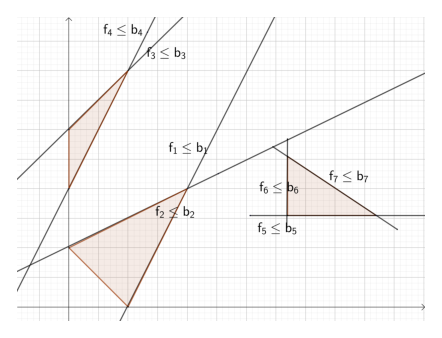
\includegraphics[width=200pt, height=180pt]{compound.eps}
	\caption{Dopustiv region sa više disjunktnih regiona.}
	\label{fig:compound_regions}
\end{figure}
Uslov $y_1 + y_2 + y_3 \leq 2$ nam upravo ograničava da rješenje $(x_1, x_2)$ pripada barem jednom od (disjunktnih) dopustivih regiona. Npr. ako je $y_3 = 0$, onda je svako od ograničenja $$f_5(x) \leq b_5, \ f_6(x) \leq b_6 \mbox{ i } f_7(x) \leq b_7$$
ispunjeno. 

%\emph{Predstavljanje nekih nelinearnih funkcija}.

\subsection{Fiksne cijene u funkciji cilja}

 Kod nekih problema, funkcija cilja problema minimizacije može da sadrži i neke fiksne troškove, kao što su fiksni troškovi ulaganja ili fiksni troškovi postavljanja opreme. Npr. trošak proizvodnje $x$ jedinica određenog proizvoda može da se sastoji od fiksnih troškova postavljanja opreme i promjenjivih troškova koji se tiču proizvedene robe na opremi (mašinama). Pretpostavimo da oprema ima kapacitet proizvodnje od $B$ jedinica (nekog proizvoda). Neka je $y$ binarna promjenljiva koja ukazuje na to kada nastaje fiksni trošak, pri čemu  je $y=1$ ako je $x >0$, dok je $x=0$ ako je $y=0$. Tada se doprinos cijeni proizvodnje od $x$ jedinica proizvoda može predstaviti sa
$$ yB + c x $$ pod uslovima:
\begin{align}
	&x \leq By \\
	& x \geq 0 \\
	& y \in \{0, 1\}.
\end{align}
Primijetimo da je ovaj model pripada \emph{Mješovitom-cjelobrojnom programiranju}, gdje postoje obje vrste promjenljivih, neprekidne i cjelobrojne. O ovoj paradigmi će biti više riječi u narednim sekcijama. 

\subsection{Po-dijelovima-linearna funkcija} 

 Po-dijelovima-linearna funkcija sama po sebi nije linearna. Međutim, kada joj se domen podijeli na segmente (intervale), ona postaje linearna na svakom od tih segmenata. Napomenimo da se svaka neprekidna relana funkcija može aproksimirati skupom po-dijelovima-linearnih funkcija.  

Radi jednostavnosti, posmatrajmo primjer zadat u ravni. Pretpostavimo da je funkcija definisana preko tri linearne funkcije na sljedeći način.
$$f(x) = \begin{cases}
	c_1 x, \mbox{ za } x \in I_1 = [\delta^1_1, \delta^1_2] \\
	c_2 x, \mbox{ za } x \in I_2 = [\delta^1_2 = \delta^2_1, \delta^2_2] \\
	c_3 x, \mbox{ za } x \in I_3 = [\delta^2_2 = \delta^3_1, \delta^3_2].
\end{cases}
$$
gdje su $I_1, I_2$ i $I_3$  zatvoreni intervali u $\mathbb{R}$, koji se nadovezuju jedan na drugi.

Da bi se modelovala ovakva funkciju cilja, promjenljivu $x$ izrazimo preko tri nove promjenljive 
$$x = \beta_1 + \beta_2 + \beta_3$$
pod uslovima 
\begin{align}
	&0   \leq \beta_1 \leq \delta^1_2 - \delta^1_1 = b_1 \nonumber \\
	&0  \leq \beta_2 \leq \delta^2_2 - \delta^2_1 = b_2 \nonumber \\
	&0  \leq \beta_3 \leq \delta^3_2- \delta^3_1 = b_3, \label{eq: piecewise-constraints}
\end{align}
odakle slijedi da je funkcija cilja   jednaka 
$$ C = c_1 \beta_1 + c_2 \beta_2 + c_3 \beta_3.$$ 
Primijetimo da se pojavljuju problemi na graničnim uslovima intervala, dakle u tačkama $I_1 \cap I_2 =\{\delta^1_2\}$ i $I_2 \cap I_3 =\{\delta^2_2\}$. Trebalo bi da vrijedi da $\beta_1 =  \delta^1_2 - \delta^1_1$ kad god je $\beta_2  > 0$ kao i $\beta_2 =  \delta^2_2 - \delta^2_1$ kad god je $\beta_3  > 0$.  S obzirom da su ovo uslovna ograničenja, ona se modeluju uvođenjem dodatnih binarnih promjenljivih 
$$ \omega_1 = \begin{cases}
	1, \mbox{ ako } \beta_1 \mbox{ dostiže svoju gornju granicu} \\
	0, \mbox{ inače},
\end{cases}$$
te 
$$ \omega_2 = \begin{cases}
	1, \mbox{ ako } \beta_2 \mbox{ dostiže svoju gornju granicu} \\
	0, \mbox{ inače}, 
\end{cases}$$
pa se ograničenja (\ref{eq: piecewise-constraints}) mogu napisati u obliku

\begin{align}
	& b_1 \omega_1 \leq \beta_1 \leq b_1   \nonumber \\
	& b_2 \omega_2 \leq \beta_2 \leq \omega_1 b_2 \nonumber \\
	& 0 \leq \beta_3  \omega_2 \leq b_3\nonumber \\
	& \omega_1, \omega_2 \geq 0. \label{eq: piecewise-constraints-equivalent}
\end{align}

Primijetimo da, ako $\omega_1 = 0$, onda je $\omega_2= 0$ kako bi se održala dopustivost za ograničenja propisana  od strane $\beta_2$, pri čemu se uslovi u (\ref{eq: piecewise-constraints-equivalent}) prevode u
$$ 0 \leq \beta_1 \leq b_1, \beta_2 =0, \beta_3 =0.$$
Ako je $\omega_1 = 1, \omega_2 = 0$, onda se uslovi u (\ref{eq: piecewise-constraints-equivalent}) transformišu u
$$   \beta_1 = b_1, 0 \leq \beta_2 \leq b_2, \beta_3 =0.$$
Ako je $\omega_1 = \omega_2 = 1$, onda se  uslovi u (\ref{eq: piecewise-constraints-equivalent}) transformišu u
$$ \beta_1 = b_1, \beta_2 = b_2, 0 \leq \beta_3 \leq b_3.$$
Prema tome, postoje tri dopustive kombinacije parametara $\omega_1$ i $\omega_2$:
\begin{itemize}
	\item  $\omega_1 = 0, \omega_2= 0$ za koje je $x \in I_1$ jer $\beta_2=\beta_3=0$;  
	\item $\omega_1 = 1, \omega_2 = 0$ za koje je $x\in I_2$, jer je $\beta_1=b_1, \beta_3=0$;
	\item $\omega_1 = 1, \omega_2 = 1$ za koje je $x\in I_3$, jer je $\beta_1=b_1, \beta_2=b_2$.
\end{itemize}
%https://download.aimms.com/aimms/download/manuals/AIMMS3OM_LinearProgrammingTricks.pdf
%https://download.aimms.com/aimms/download/manuals/AIMMS3OM_IntegerProgrammingTricks.pdf

% \emph{Eliminacija proizvoda varijabli}.

\subsection{Eliminacija proizvoda promjenljivih}

Jasno je da proizvod dvije ili više promjenljivih narušavaju linearnost modela, te je korisno poznavati mehanizam kako se takvi proizvodi mogu izbjeći, odnosno transformisati u odgovarajuće linearizovane relacije. U ovom odjeljku ćemo prezentovati kako se proizvod dvije promjenljive može zamijeniti jednom promjenljivom  sa dodatnim ograničenjima. Taj metod se, po potrebi, može proširiti i na proizvod više od dvije promjenljive. Razlikujemo nekoliko slučajeva:
\begin{itemize}
	\item $x_1$ i $x_2$ su binarne promjenljive. Uvedemo smjenu $y=x_1 x_2$, uz sljedeće uslove za promjenljivu $y$:
	\begin{align*}
		&y \leq x_1 \\
		&y \leq x_2 \\
		& y \geq x_1 + x_2 - 1 \\
		& y \in \{0, 1\}.
	\end{align*}
	
	Ova tehnika se može generalizovati na slučaj kada imamo proizvod $n$ binarnih promjenljivih. Definišimo promjenljivu  $y = x_1 \cdot \ldots \cdot x_n$, $x_i\in\{0,1\}, i=1,\ldots ,n$. Uključivanjem sljedećih ograničenja 
	\begin{align*}
		&y \leq x_1 \\
		& \vdots \\
		&y \leq x_n \\
		& y \geq \sum_{i=1}^n x_i - (n-1) \\
		& y \in \{0, 1\}.
	\end{align*}
	postiže se tražena transformacija.
	
	\item $x_1$ je binarna, $x_2$ je realna (pozitivna) promjenljiva, $0 \leq x_2 \leq u$. Opet uvodimo istu smjenu $y= x_1 x_2$, gdje je $y$ neprekidna promjenljiva. Dodamo sljedeća ograničenja, kako bismo osigurali da $y$    dobije vrijednost proizvoda:
	\begin{align*}
		&y \leq u x_1 \\
		&y \leq x_2 \\
		& y \geq x_2 - u(1-x_1) \\
		& y \geq 0.
	\end{align*}
	
	\item $x_1, x_2$ su obje neprekidne promjenljive, $l_1 \leq x_1 \leq u_1$, $l_2 \leq x_2 \leq u_2$. Uvedemo promjenljive $y_1 = \frac{1}{2}( x_1 + x_2) $ i  $y_2 =\frac{1}{2}(x_1 - x_2)$. Tada se izraz $x_1x_2$ može predstaviti u separabilnoj formi $y_1^2 - y_2^2$ koja se zatim može aproksimirati po-dijelovima-linearnim funkcijama. Granice za vrijednosti novih promjenljivih su 
	$$ \frac{1}{2}(l_1 + l_2) \leq y_1 \leq \frac{1}{2}(u_1 + u_2)$$ i 
	$$ \frac{1}{2}(l_1 - u_2) \leq y_2 \leq \frac{1}{2}(u_1 - l_2) $$
	
\end{itemize} 

%\fixme{marko, ovaj donji paragraf mi je nejasan. U kojoj prethodnoj stavci je pomenuta aproksimacija pomocu niza po dijelovima linearnih funkcija? Marko: Izgleda obrisano, pomenuto sada u 6.2.7. stavka (ii) }

\emph{Aproksimacija nelinearnih funkcija}. Kako smo pomenuli u prethodnoj sekciji, ako je funkcija cilja realna, neprekidna i nelinearna, ona se može aproksimirati uz pomoć  niza po-dijelovima-linearnih funkcija. Na tu aproksimaciju ćemo potom primjeniti transformaciju ograničenja koja je već prezentovana u prethodnoj sekciji, a tiče se po-dijelovima-linearnim funkcijama. 

U sljedećem primjeru primijenimo nekoliko navedenih transformacija ograničenja.


\begin{primjer} Pretpostavimo da je stanovništvo koncentrisano u $I$ okruga  unutar grada i da u okrugu $i\in [I]$ stanuje $p_i$ ljudi. Preliminarna analiza (premjeri zemljišta, političke i društvene prilike itd.) dala je potencijalne lokacije za izgradnju vatrogasnih domova na $J$ lokacija. Neka $d_{ij} \geq 0$ predstavlja udaljenost   središta okruga (dijela grada) $i$  do lokacije $j \in J $. 
\end{primjer}
Zadatak: \emph{Potrebno je odabrati lokacije gdje će se podići vatrogasni domovi za svaki od okruga. O funkciji cilja i dodatnim ograničenjima ćemo diskutovati u toku modelovanja samog problema.}

Definišimo binarne promjenljive 
$$y_j = \begin{cases}
	1, \mbox{ ako je lokacija } j \mbox{ odabrana za izgradnju doma} \\
	0, \mbox{ inače}
\end{cases}$$
i 
$$
x_{ij}= \begin{cases}
	1, \mbox{ ako je lokacija za vatrogasni dom } j \mbox{ nadležna za okrug } i \\
	0, \mbox{ inače}. 
\end{cases}
$$
Svaki okrug treba da bude pridružen tačno jednom vatrogasnom domu, pa se to ograničenje modeluje sa
\begin{equation}\label{eq:ex-constr-1}
	\sum_{j \in J} x_{ij} = 1, \forall i \in I
\end{equation}
Takođe, ako lokacija za vatrogasni dom nije odabrana, onda nijedan okrug nije pridružen toj lokaciji. Odnosno, ako je $y_j = 0$, onda $ \sum_{i \in I} x_{ij} = 0$. Ovo je uslovno ograničenje, koje se modeluje sa
\begin{equation}\label{eq:ex-constr-2}
	\sum_{i \in I} x_{ij} \leq y_j |I|.
\end{equation}
%gdje je $|I|$ broj mijesta. 

Udaljenost okruga $i$ do nadležnog vatrogasnog doma je jednaka $d_i = \sum_{j \in J} d_{ij}x_{ij} $. Dalje, veličina populacije (broj ljudi) koja će biti pod nadzorom od strane doma na lokaciji $j$ je jednaka 
\begin{equation}\label{eq:ex-constr-3}
	s_j = \sum_{i \in I} p_i x_{ij}. 
\end{equation}
Pretpostavimo da je jedan okrug posebno osjetljiv na požar i da lokacije  1 i 2 ili lokacije 3 i 4 treba  da budu iskorištene da zaštite taj okrug. Ovakva situacija se modeluje sa ograničenjima
\begin{equation*} 
	y_1 + y_2 \geq 2 \mbox{ ili } y_3 + y_4 \geq 2
\end{equation*}
što je ekvivalentno sa 
\begin{align}
	&y_1 + y_2 \geq 2 z \nonumber \\
	&y_3 + y_4 \geq 2 (1-z) \nonumber \\
	& z\in \{0, 1 \}.\label{eq:ex-constr-4}
\end{align}
Pretpostavimo da cijena izgradnje vatrogasnog doma na mjestu $j$ koje može voditi brigu o $s_j$ ljudi košta $f_j(s_j)$. Pretpostavimo takođe da je budžet kojim raspolažemo jednak $B$. Prema tome, vrijedi ograničenje
\begin{equation}\label{eq:ex-constr-5}
	\sum_{j \in J} y_j f_j(s_j) \leq B.
\end{equation}
Funkcija cilja koja bi se mogla optimizovati u ovoj varijanti problema je minimizacija udaljenosti 
okruga koja je najudaljenija od svog nadležnog vatrogasnog doma (označeno sa $d_i$)
$$\min D $$
gdje je $D= \max d_i$. Ova funkcija cilja se može napisati  u ekvivalentnom obliku kao:
\begin{align*}
	&\min D \\     
	&  \mbox{t.d.} \\
	& D \geq d_i,  \forall i \in I \\
	&(\ref{eq:ex-constr-1})-(\ref{eq:ex-constr-5}) \\
	& D \in \mathbb{R}^+. 
\end{align*}
Kako bismo završili modelovanje, ostalo je još da se svaka funkcija $f_j (s_j)$ zamijeni aproksimacijom cjelobrojnog programiranje. Detalje ostavljamo čitaocu kao zadatak. Ako bi funkcija $f_j (s_j)$ sadržala fiksne troškove, tada se ne bi trebale uvoditi nove promjenljive fiksnih troškova, jer u tu svrhu već služi ranije uvedena promjenljiva $y_j$. 
% jos neki trikovi u modelovanju: https://download.aimms.com/aimms/download/manuals/AIMMS3OM_LinearProgrammingTricks.pdf

\section{Kompleksnost rješavanja cjelobrojnog programiranja}\label{sec:kompleksnostILP}

Na početku ove glave smo pomenuli da je rješavanje problema cjelobrojnog programiranja NP--težak problem. Napomenimo da to nije slučaj sa problemom linearnog programiranja, za koji smo u Glavi~\ref{chp:dualnost} pokazali da je rješiv u polinomijalnom vremenu. U nastavku ove sekcije dajemo dokaz da je rješivost ILP-a zaista NP--težak problem. Ideja dokaza je da problem 3--SAT  polinomijalno svedemo na ILP.
%https://mediaspace.msu.edu/media/Proving+that+Integer+Programming+is+NP-Complete/1_0j1vkmvw
Podsjetimo se definicije 3--SAT problema. 

Neka su dati literali $x_1, \ldots, x_n$. Svaki literal može da bude pozitivan ($x_1$) ili negativan  ($\neg x_1$). Kažemo da je formula napisana u \emph{konjunktivnoj normalnoj formi} (CNF) akko je napisana kao konjunkcija klauzula ili literala. Pod klauzulom podrazumijevamo formulu koja je sastavljen  od literala povezanih disjunkcijama. Npr. formula $\phi(x_1, x_2, x_3)= (x_1 \vee  \neg x_2) \wedge (x_1 \vee x_3)$ je napisana u CNF. Ona se sastoji od dvije klauzule sastavljena od po dva literala. CNF formula $\phi(x)$ je zadovoljiva akko postoji dodjela $\overline{x}$ literalima ($\overline{x}_i \in \{TRUE, FALSE\}$) tako da je $\phi(\overline{x})$ tačna, prema zakonima Bulove algebre.  


Kažemo da je konjunktivna formula $\phi(x)$  napisana u 3--CNF  akko se u svakoj klauzuli nalazi najviše 3 različita literala. Napomenimo da se, u smislu rješivosti, proizvoljna klauzula može redukovati u 3--CNF. Dakle, svaka klauzula 
$l_1 \vee l_2 \vee \cdots \vee l_n$ se može pretvoriti u 3--CNF na sljedeći način:
\begin{align*}
	&(l_1 \vee l_2 \vee x_2) \wedge ( \neg x_2 \vee l_3 \vee x_3) \wedge ( \neg x_3 \vee l_4 \vee x_4 ) \wedge \cdots \wedge (\neg x_{n-3} \vee l_{n-3} \\
	&\vee x_{n-2} ) \wedge ( \neg x_{n-2} \vee l_{n-1} \vee l_n ),  
\end{align*}    
gdje su $x_2, \ldots, x_{n-2}$  proizvoljne bulove promjenjive (literali).  

Treba imati na umu da ove formule nisu logički ekvivalentne, ali su ekvivalentne u smislu zadovoljenja. Dakle, ako je jedna od formula zadovoljiva za neku dodjelu logičkih vrijednosti literalima, onda je to i druga, i obrnuto. 
Poznato je da je problem 3--SAT, gdje je ulaz 3--CNF formula,  u opštem slučaju NP-kompletan problem.  

\begin{thm}
	Problem ILP-a je NP-težak.
\end{thm}
\begin{proof}
	Izvedimo polinomnu redukciju instance 3-SAT problema na instancu problema ILP-a. Neka je dat 3--SAT izraz sa literalima  
	$x_1,\ldots, x_n$.  Konstruišimo ILP instancu sa promjenljivima $z_1, \ldots, z_n$.
	Svaka klauzula $\phi_i(x)$ se pretvara u nejednakost (ograničenje)  $C_i$ na sljedeći način:
	\begin{itemize}
		\item $z_i = x_i$, ako se literal $x_i$ pojavljuje u klauzuli $\phi_i$; 
		\item $z_i = 1 - x_i$ ako se $\neg x_i$ pojavljuje u klauzuli $\phi_i$;
		\item znak disjunkcije se mijenja znakom sabiranja ,,+'';
		\item vrijednost konstruisanog izraza treba da bude $\geq 1$. 
	\end{itemize}
	Primjera radi, ako je data instanca problema 3-SAT sa 
	$\phi(x) = (x_1 \vee \neg x_2 \vee \neg x_3) \wedge ( x_2 \vee \neg x_4 \vee x_5 )$, transformišemo je (u polinomnom vremenu) na instancu ILP-a
	\begin{align*}
		& \min f \\
		&C_1: z_1 + (1- z_2) + (1 - z_3 ) \geq 1 \\
		& C_2: z_2 + (1-z_4)  + z_5 \geq 1 \\
		& C_3: z_i \in \{0,1\}, i=1,\ldots,5.
	\end{align*} 
	%%https://cims.nyu.edu/~regev/teaching/lattices_fall_2004/ln/integer_programming.pdf :Aco
	Dakle, iz gornje redukcije,  provjera dopustivosti ILP instance odgovara provjeri zadovoljivosti 3--CNF izraza $\phi$.   Prema tome, problem rješivosti ILP-a je NP-težak, s obzirom da je 3--SAT problem NP-kompletan. 
\end{proof} 
Može se pokazati i sljedeća teorema.
\begin{thm} Neka je $k\in \mathbb{Z}$.
	Problem odlučivanja da li postoji cjelobrojno dopustivo rješenje  ILP-a  vrijednosti manje od $k$ je NP--kompletan.
\end{thm}

\section{Zadaci}
\begin{enumerate}
	
	\item Preduzeće za prikupljanje reciklažnog otpada raspolaže sa dvije deponije, koje su označene sa A i B. Dnevni troškovi održavanja deponije A su 300KM, a deponije B 45KM.  U deponiji A se dnevno prikupi 250 flaša i 100 limenki, dok se u deponiji B prikupi 160 flaša i 350 limenki. Da bi se isplatio rad deponija, mjesečno treba prikupiti barem 5200 flaša i 4000 limenki.
	Koliko bi dana mjesečno trebale raditi obje deponije da budu isplative i da troškovi budu minimalni?
	
	\item Fabrika proizvodi artikle A i B te ih prodaje po cijeni 30 KM, odnosno 50 KM, po komadu. Za
	proizvodnju fabrika koristi samo jednu mašinu, pri čemu je za proizvodnju artikla A potrebno 19
	minuta, a proizvoda B 26 minuta. Tokom dana aparat može da radi najviše 8 sati. Odredi koliko treba
	proizvesti proizvoda A, a koliko B, da bi zarada bila maksimalna.
	
	\item Aleksandar se sprema na planinarenje. Na raspolaganju ima samo jedan ruksak i pet namirnica, po jedan
	komad svake od njih. Ruksak je kapaciteta 2.5 $l$ i ne smije biti teži od 2 $kg$. U tabeli su
	prikazani podaci o namirnicama.
	\begin{table}[H]
		\centering
		\scalebox{0.85}{
			\begin{tabular}{|c|c|c|c|}
				\hline
				Namirnica & Masa (g) & Zapremina (L) & Kalorijska vrijednost (kcal) \\
				\hline
				Čokolada & 300 & 0,5 & 1500 \\
				\hline
				Kokos & 500 & 1,4 & 1300 \\
				\hline
				Mlijeko& 1000 & 1 & 660 \\
				\hline
				Pasulj u konzervi& 400 & 0,8 & 650 \\
				\hline
				Keks& 500 & 0,9 & 1800 \\
				\hline
		\end{tabular}}
	\end{table}
	Kako treba napuniti ruksak da ukupna kalorijska vrijednost ponesenih namirnica bude maksimalna?
	
	\item Riješiti prethodni zadatak ako Aleksandar na raspolaganju ima dovoljno veliki broj svih pojedinačnih namirnica.
	
	
	\item Preduzeće  razmatra izvođenje 5 trogodišnjih projekata, ali u svakoj godini može uložiti najviše
	25 000 KM. Procjena troškova, u hiljadama maraka, za svaki projekat u tri godine, kao i
	očekivana dobit od projekta (čista dobit – troškovi su oduzeti)  dati su tabelom:
	%	\begin{table}
		%	\centering
		\begin{center}
			
			\begin{tabular}{|c|c|c|c|c|}
				\hline
				Projekat & 1. godina & 2. godina & 3. godina & Dobit \\
				\hline
				1 & 5 & 1 & 8 & 20 \\
				\hline
				2 & 4 & 7 & 10 & 40 \\
				\hline
				3 & 3 & 9 & 2 & 20 \\
				\hline
				4 & 7 & 4 & 1 & 15 \\
				\hline
				5 & 8 & 6 & 10 & 30 \\
				\hline
			\end{tabular}  \\
		\end{center}
		%	\end{table}
	Odrediti koje od projekata treba realizovati da se maksimizuje ukupna dobit.
	
	\item Zadat je skup $S$ koji se sastoji od $n$ brojeva. Koristeći tehnike cjelobrojnog linearnog programiranja, podijeliti skup $S$ na dva podskupa, tako da se zbirovi elemenata u prvom i drugom podskupu što manje razlikuju.
	
	\item Riješiti prethodni zadatak uz dodatni uslov da nijedan podskup ne smije da sadrži više od $\frac {2n}3$ elemenata.
	
	
	
	%https://www.utc.fr/~dnace/dokuwiki/_media/fr/upt-cours-2012lp.pdf
	\item U ovom zadatku je potrebno modelovati \emph{problem totalnog pokrivanja}. %Neka je dato $n$ mijesta, te $m$ zahtjeva koji treba da budu ispunjeni ($d_1,\ldots, d_m$).  
	Sa $D_c$ označimo maksimalnu daljinu koja se može pokriti instalacijom $c$. Pod instalacijom podrazumijevamo skladiše, antene i sl. Pod ,,pokrivanjem'' podrazumijevamo ispunjavanje zahtjeva klijenata, koji žive u nekom mjestu. Sa $c_i$ označimo cijenu postavljanja instalacije na mjesto $i$. Sa $d_{ij}$ označimo udaljenost između mjesta $i$ i $j$. Zadatak ovog problema je da se odredi koja mjesta da se odaberu za instalacije, tako da su sva (ostala) mjesta pokrivena, ali da pri tome minimizujemo troškove instalacija. Sa jednog odabranog mjesta $c$ se pokrivaju sva susjedna mjesta koja su u okviru radijusa $D_c$.  
	\item U ovom zadatku se modeluje  \emph{problem maksimalnog pokrivanja} (eng. \emph{maximum coverage problem}). Neka je na ulazu data kolekcija skupova  $S=\{ S_1, \ldots, S_m\}$ te broj $k \in \mathbb{N}$. Potrebno je naći podskup $S' \subseteq S$, tako da je $|S'|\leq k$, a broj pokrivenih elemenata $|\bigcup_{s' \in S'} s'|$ je maksimizovan. 
	
	\emph{Uputstvo}. Sa $x_j \in \{0, 1\}$ označimo promjenljivu koja dobija vrijednost 1 ako je skup $S_i$ odabran u rješenje $S'$, inače 0. Dodatno, sa $y_j \in \{0, 1 \}$ definišemo promjenljivu koja dobija vrijednost 1 ako je   element $e_j$ pokriven rješenjem.  
	%http://courses.ieor.berkeley.edu/ieor151/lecture_notes/ieor151_lec14.pdf
	\item Potrebno je modelovati \emph{$P$-center problem čvorova} (eng. \emph{vertex p-center problem}). Formulacija problema je sljedeća. Ulazni podaci su predstavljeni neusmjerenim grafom $G = (I, J, E)$, gdje su objekti potražnje predstavljeni  vrhovima $i\in I$, a moguće lokacije (servisnih) objekata su date   drugim skupom vrhova $j \in J$, Grane $e_{i,j} \in E$ postoje samo između čvorova $i \in  I$ i čvorova $j \in J$. Dalje, parovima čvorova su dodijeljene pozitivne težine $d_{i,j}\geq 0$, što predstavlja udaljenost između čvorova $i$ i $j$. Treba imati na umu da je moguće imati i udaljenost 0 između čvora potražnje i moguće lokacije objekta. Za svaki čvor $i \in I$ pridružena je težina zahtjeva $h_i>0$, koja predstavlja količinu zahtjeva koje taj čvor može da ispuni. 
	
	Zadatak je postaviti $p$ objekata kako bi se smanjila maksimalnu udaljenost između bilo kojeg čvora potražnje i	njegovog servisnog objekta. 
	\item %https://personal.utdallas.edu/~metin/Or6302/Notes/integer.pdf
	Pretpostavimo da se selimo u novi stan i da imamo samo dva kofera u koje možemo spakovati svoje stvari. U prvi kofer može da se spakuje 22 kg, a drugi 28 kg. Težina i vrijednosti stvari
	su dati sa tabelom
	\begin{table}[H]
		\centering
		\begin{tabular}{l|cccccccc}
			Stavka & A & B & C & D & E & F & G & H \\ \hline
			Težina & 10 & 9 & 15 & 3 & 11 & 6 & 3 & 4 \\
			Vrijednost & 5 & 2 & 7 & 6 & 1 & 6 & 8 & 6 \\ \hline
		\end{tabular} 
		
	\end{table}
	Konstruišite model koji maksimizuje vrijednost  predmeta koji mogu biti ubačeni u ova dva kofera. 
	\item Višedimenzionalni više-direkcioni problem particionisanja brojeva (eng. \emph{multidimensional multi-way number partitioning problem}) se definiše na sljedeći način. Neka je dat skup vektora $S$. Vektori mogu da budu iz proizvoljneg prostora $\mathbb{R}^m, m \in \mathbb{N}$.   Zadatak je podijeliti skup $S$ na $p \geq 1$ particija tako da su sume vrijednosti  elemenata  po koordinatama po particijama što ujednačenije. 
	
	\item U ovom zadatku se razmatra  \emph{Problem maksimalnog nezavisnog skupa} (eng. \emph{independent set problem}). Dat je graf $G = (V, E)$. Potrebno je naći podskup $V' \subseteq V$ maksimalne kardinalnosti takav da  $V'$ ne sadrži ni jedan par susjednih čvorova. 
	\item Problem maksimalne klike (eng. \emph{maximum clique problem}) se definiše na sljedeći način.  Dat graf $G = (V, E)$. Potrebno je naći podskup $V' \subseteq V$ maksimalne kardinalnosti tako da je indukovani podgraf 
	$G[V']$ grafa $G$ kompletan graf. 
	\item % http://people.brunel.ac.uk/~mastjjb/jeb/or/moreip.html
	Proizvođač igračaka planira proizvodnju novih igračaka. Troškovi pripreme proizvodnih pogona i jedinični profit za svaku igračku dati su sljedećom tabelom: 
	\begin{table}[H]
		\centering
		\begin{tabular}{l|cc} 
			\hline
			Igračka &  Troškovi pripreme    & Profit \\ \hline
			1       &  45000     &  12     \\
			2       &  76000     &  16     \\	\hline
		\end{tabular} 
	\end{table}
	Kompanija ima dvije fabrike koje mogu proizvoditi ove igračke. Kako bi se izbjeglo udvostručenje troškova pripreme za proizvodnju,  samo jedna fabrika se može koristiti u datom momentu. 
	
	
	Stope proizvodnje svake igračke date su tabelom (u jedinicama/satu): 
	\begin{table}[H]
		\centering
		\begin{tabular}{l|cc} \hline
			\        &  Igračka 1 & Igračka 2 \\ \hline
			Fabrika 1   &  52     &  38     \\
			Fabrika 2   &  42     &  23     \\	\hline
		\end{tabular} 
	\end{table}
	Fabrika 1 i 2, imaju 480 i 720 sati radnog vremena za proizvodnju ovih igračaka, respektivno. Proizvođač želi znati koju će od novih igračaka proizvesti, u kojoj tvornici i koliko svake (ako uopšte) treba proizvesti kako bi se ukupna zarada maksimizovala. 
	\item %http://people.brunel.ac.uk/~mastjjb/jeb/or/moreip.html
	Hrana se proizvodi rafiniranjem sirovih ulja i njihovim miješanjem. Postoje dvije kategorije sirovog ulja: 
	\begin{itemize}
		\item vegansko ulje:
		\begin{enumerate}
			\item VEG1
			\item VEG2 
		\end{enumerate}
		\item obično ulje:
		\begin{enumerate}
			\item Ulje1
			\item Ulje2 
			\item Ulje3
		\end{enumerate}
	\end{itemize}
	Cijene za kupovinu svakog ulja date su u nastavku (u KM/toni)
	\begin{table}[H]
		\centering
		\begin{tabular}{ccccc}
			VEG1 & VEG2 & Ulje1 & Ulje2 & Ulje3 \\ \hline
			115  & 128  & 132   & 109   & 114 \\ 	\hline	
		\end{tabular} 
	\end{table}
	Finalni proizvod prodaje se po 180 KM po toni. Biljna ulja i ne-biljna ulja zahtijevaju različite proizvodne linije za rafinisanje. Nije moguće rafinisati više od 210 $t$ biljnih ulja i više od 260 $t$ nebiljnih ulja. Pretpostavimo da u procesu rafinisanja nema gubitka težine, a troškovi prerade mogu se zanemariti. 
	
	Postoji tehničko ograničenje koje se odnosi na tvrdoću konačnog proizvoda. U jedinicama u kojima se mjeri tvrdoća, dopušteno je da ona ima vrijednosti između 3.5 i 6.2. Pretpostavlja se da se tvrdoća mijenja %odnosi
	linearno sa miješanjem vrsta ulja. Tvrdoća sirovog ulja je data sljedećom tabelom
	\begin{table}[H]
		\centering
		\begin{tabular}{ccccc}
			VEG1 & VEG2 & Ulje1 & Ulje2 & Ulje3 \\ \hline
			8.8  & 6.2  & 1.9   & 4.3   & 5.1   \\
		\end{tabular} 
	\end{table}
	
	Potrebno je odrediti koja ulja kupiti i kako ih miješati  tako da kompanija maksimizuje svoj profit. 
	
	U osnovni model uključiti i sljedeća ograničenja:
	\begin{itemize}
		\item Hrana nikad ne smije biti  pravljena miješanjem više od 3 vrste ulja. 
		\item Ako je neko ulje uključeno u upotrebu,  koristi se barem 30 $t$ tog ulja.
		\item Ako su ulja VEG1 ili VEG2  korištena, onda i Ulje2 mora biti korišteno.  
	\end{itemize}
	
\end{enumerate}                                                       

 \chapter{Algoritamske tehnike za rješavanje Cjelobrojnog linearnog programiranja}\label{chap:rjesavanjeILP}
 
 U ovom poglavlju će biti analizirane različite tehnike kojima se rješavaju problemi cjelobrojnog linearnog programiranja.
 Za razliku od problema LP-a, koji se efikasno rješava simpleks metodom, za rješavanje problema cjelobrojnog linearnog programiranja ne postoji generalno efikasna metoda. Drugim riječima, efikasnost metoda, kojima se rješava ovaj problem, u velikoj mjeri zavisi od karakteristika samog problema. 
 
Tehnike za rješavanje su uglavnom zasnovane na tzv. relaksaciji ILP-a u odgovarajući LP, koji se od polaznog problema (ili nekog od podproblema generisanog u toku rješavanja) dobija zanemarivanjem uslova o cjelobrojnosti promjenljivih.  Iako se dobijena  LP relaksacija može efikasno riješiti uz pomoć simpleks metoda, to ne znači da se iz rješenja relaksacije može lako doći do rješenja polaznog ILP-a. Npr. ako rješenje LP relaksacije označimo sa $x^*$, zaokruživanjem svake koordinate vektora $x^*$ na njenu najbližu cjelobrojnu vrijednost, dobijamo cjelobrojni vektor  $\overline{x}$.  U uvom slučaju, uslov cjelobrojnosti jeste zadovoljen, ali ne postoji nikakva garancija da će, u opštem slučaju,  ovakvo rješenje izvedeno iz LP relaksacije problema (\ref{ilp-formulation}), biti i  dopustivo za početni ILP. Pored toga, skaliranjem desnih strana ograničenja ILP-a, kao i koeficijenata funkcije cilja na odgovarajući način, moguće je konstruisati problem, čije je optimalno cjelobrojno rješenje proizvoljno udaljeno od zaokruženog rješenja LP relaksacije. 
 
 Razmatranje opisano u prethodnom paragrafu ukazuje na to da se, uz relaksaciju početnog ILP-a u LP, moraju koristiti suptilnije tehnike za određivanje optimalnog rješenja ILP-a. 
 
Metode za egzaktno rješavanje ILP-a se mogu klasifikovati na sljedeći način:
 \begin{enumerate}
     \item \emph{Enumerativne tehnike} -- dinamičko programiranje, metoda granjanja i ograničavanja (eng. \emph{branch-and-bound} -- B\&B), metoda implicitne enumeracije i druge;
     \item \emph{Tehnike odsjecajućih ravni}.
     %\item Grupne-teoretske tehnike. 
 \end{enumerate}


\section{Metoda grananja i ograničavanja (B\&B)}\label{sec:bb}
Metoda grananja i ograničavanja  je zasnovana na poznatom principu ,,zavadi pa vladaj'' (eng. divide and conquer) gdje se problem, rekurzivno, rastavlja na manje dijelove. Kasnije se (optimalna rješenja) manjih problema kombinuju na odgovarajući način za dobijanje optimalnog rješenja početnog problema.  U B\&B metodi važan dodatak je upotreba strategije da se 
problem nikada ne rastavlja na manje podprobleme ako se može procijeniti da će rješenje podproblema biti suboptimalno (ograničavanje). Drugim riječima, algoritam ,,ne ulazi'' u one grane, za koje se unaprijed može pokazati da sadrže samo  rješenja koja su lošija od trenutno najboljeg dopustivog rješenja. Očigledno, na taj način dolazi do uštede u broju operacija koje je potrebno izvršiti u toku izvođenja algoritma, a, samim tim, dolazi i do uštede memorije i vremena izvršenja. U rješavanju ILP-a, dopustiv skup se dijeli na manje skupove, dodavanjem specijalnih ograničenja u model. Rekurzivni postupak se izvršava sve  dok se ne dobiju podproblemi, čije relaksacije obezbjeđuju cjelobrojno rješenje ili se zaključi da podproblemi nisu dopustivi. Ovakvi pristupi se razlikuju u načinu podjele dopustivog skupa i zbog toga  u literaturi  postoji nekoliko različitih B\&B procedura. 

\subsection{Bazni B\&B za rješavanje problema ILP-a}

U rješavanju problema  ILP-a uz pomoć B\&B procedure, sljedeće jednostavne činjenice mogu biti korisne:
\begin{itemize}
    \item  U LP relaksaciji (problema 
           maksimizacije), optimalna vrijednost  relaksacije  će biti gornja granica (eng. upper bound, skraćeno $UB$) optimuma posmatranog ILP-a na odgovarajućem podregionu. 
    \item  Bilo koja cjelobrojna tačka LP relaksacije na nekom podskupu  
           dopustivog skupa uvijek je  donja granica (eng. lower bound, skraćeno $LB$) optimalne vrijednosti početnog ILP-a. 
\end{itemize}
%Definišimo $LB = - \infty$. 
Na osnovu ove dvije činjenice, uvedimo sada sistematičnu podjelu dopustivog regiona na niz podregiona:
\begin{enumerate}
    \item U korjenom čvoru B\&B stabla rješavamo LP relaksaciju početnog problema     (npr. simpleks metodom) i dobijamo rješenje $x^*=(x^*_1, \ldots, x^*_n)$.   Ako je rješenje cjelobrojno, prekidamo dalje izvršavanje i stavimo $LB=f(x^*)$, koje je optimalno. %U protivnom, postavimo $f(x^*)=UB$.
    \item Za sve koordinate $i$ za koje je $x^*_i \not \in \mathbb{Z}$, dopustiv region se može podijeliti na dva (disjunktna) podskupa uvođenjem ograničenja: $z_i \geq \lfloor x^*_i \rfloor + 1$ ili $z_i \leq \lfloor x^*_i \rfloor$ i to je upravo mjesto podjele dopustivog regiona. Ako ima više takvih koordinata, biramo onu koordinatu kojoj je decimalni dio najveći.  Recimo da je to koordinata $k$.
    \item Sada dijelimo region problema na dva podregiona (lijevi i desni potomak čvor u B\&B drvetu), dodavajući 
          ograničenja $x_k \geq \lfloor x^*_k \rfloor + 1$ i $x_k \leq \lfloor x^*_k \rfloor$, redom.
    \item Rješavamo relaksaciju oba (pod)problema i razmatramo sljedeće slučajeve. 
    \begin{itemize}
    	\item  Ako je neko od rješenja cjelobrojno, popravljamo $LB$ (ako smo dobili bolje dopustivo rješenje) i odgovarajući podproblem (njegov region) se dalje ne dijeli. 
    	\item Ako rješenje $x$ nije cjelobrojno i pri tome je vrijednost optimuma manja od trenutne $LB$, taj podproblem se dalje više ne dijeli (\emph{bound} procedura). 
    	\item Dalje, ako je podproblem nedopustiv, problem se ne dijeli (i ne razmatra više). 
    	\item Inače, idemo na korak 2 dijeljeći podregion   na nove (manje) podregione nekog od podproblema za koje to nije urađeno.    
    \end{itemize}

\end{enumerate}

Primijetimo da ovom metodom formiramo drvo enumeracije koje nam garantuje nalazak optimalnog rješenja početnog ILP-a. Takođe, primijetimo da ovo drvo u generalnom slučaju raste eksponencijalno u odnosu na veličinu ulaznog problema.  

  Ovo je bila okvirna shema B\&B procedure. Ono što je ostalo nerazjašnjeno je koji od neriješenih podproblema prvo rješavati. Kažemo da se čvorovi čiji je odgovarajući problem podijeljen na podregione naziva \emph{neaktivan}, a inače \emph{aktivan}. Generalni B\&B metod za rješavanje problema ILP-a je dat   Algoritmom~\ref{bnb_algorithm_ilp}.  Neki od kriterijuma za izbor čvora (podproblema) koji se rješava su sljedeći:
  \begin{itemize}
  	\item Izabrati one aktivne čvorove koji su najdublje u drvetu, da bi se što prije stiglo do listova B\&B stabla i potencijalnih dopustivih rješenja.
  	\item Birati aktivne čvorove nivo po nivo. Dakle, sve aktivne čvorove (tj. odgovarajuće podprobleme) jednog nivoa   rješavati, pa onda preći na čvorove narednog nivoa. 
  	\item Koristiti heurističku funkciju pri odlučivanju koji aktivni čvor (tj. odgovarajući podproblem) prvo rješavati. 
  \end{itemize}

\begin{algorithm}[!htb] 
	\begin{algorithmic}[1] 
		\STATE $LB \gets$ $-\infty$
		\STATE Početni problem je aktivan (korjeni čvor)
		\WHILE{postoji neki aktivni čvor}
		\STATE  $v_j \gets$ Odabrati neki od aktivnih čvorova; // strategija
		\STATE  Označiti $v_j$ kao neaktivan;
		\STATE  $x^j \gets$ Riješiti relaksaciju podproblema koji odgovara čvoru $v_j$
		\STATE $z^*_j \gets f(x^j)$;
		\IF{ $z^*_j  \leq LB$} 
		\STATE Čvor $j$ nije relevantan za dalje razmaranje; 
		\ENDIF
		\IF{$z^*_j  > LB$}
		\IF{$x^j$ je dopustivo}
		\STATE $LB \gets z^*_j$;
		\STATE $x^* \gets x^j$;
		\ELSE 
		%\IF{$z^*_j  > LB$} // nije dopustivo
		%\IF{$x^j$ nije dopustivo}
		\STATE $v_j^{'}, v_j^{''},\ldots, v_j^{(')^k}  \gets$ Generisati podprobleme (čvorove) problema koji odgovara problemu čvora $v_j$ (branch procedura);
		\STATE Označi aktivnim nove čvorove; 
		\ENDIF
		\ENDIF
		\ENDWHILE
	\end{algorithmic}
	\caption{Generalni B\&B za rješavanje ILP-a.}\label{bnb_algorithm_ilp}
\end{algorithm}
\begin{primjer}
Na Slici~\ref{fig:bnb_ilp} je prikazano B\&B drvo sljedećeg ILP-a:
\end{primjer}
\begin{align*}
    &\max 5 x_1 + 8 x_2 \\
    &x_1 + x_2 \leq 6 \\
    & 5 x_1 + 9 x_2 \leq 45 \\
    & x_1, x_2 \geq 0\\
    & x_1,x_2 \in \mathbb{Z}.
\end{align*}

%\begin{figure}
%    \centering
%    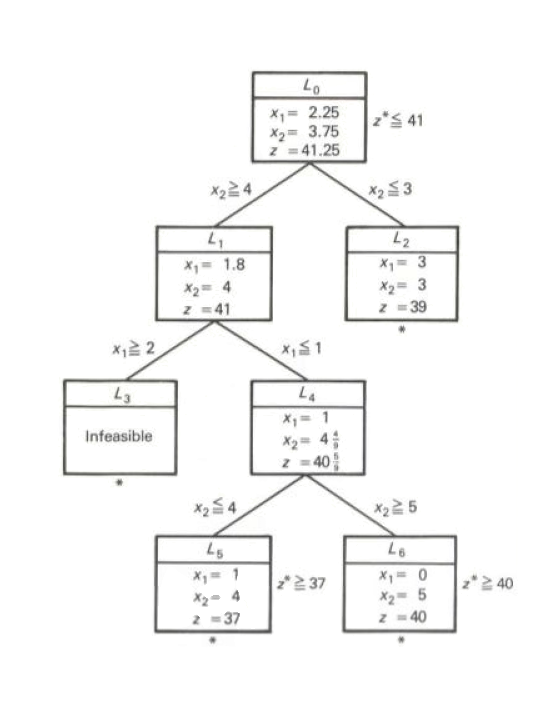
\includegraphics[width=200pt, height=200pt]{bnb_ilp.eps}
%    \caption{B\&B stablo ILP problema.}
%    \label{fig:bnb_ilp}
%\end{figure}

\begin{figure}[!ht]
	\centering
	\begin{tikzpicture}
		\node[parent node,rectangle split parts=1](A){\textA};
		%\node[parent node,below =of A](B){\textB};
		\node[parent node,below left =of A](B){\textC};
		\node[parent node,below right =of A](C){\textD};
		\node[parent node,node distance=1 and 0.3,below left =of B](D){\textE};
		\node[parent node,node distance=1 and 0.3,below right =of B](E){\textF};
		\node[parent node,node distance=1 and 0.3,below left=of E](G){\textG};
		\node[parent node,node distance=1 and 0.3,below right=of E](H){\textH};
		%\draw[->](A.south)--(B)node[midway,right]{\scriptsize solve as continous problem};
		\draw[->](A.south)--+(0,-0.5)-|(B)node[right,near end]{\scriptsize $x_2\geq 4$};
		\draw[->](A.south)--+(0,-0.5)-|(C)node[left,near end]{\scriptsize $x_2\leq 3$};
		\draw[->](B.south)--+(0,-0.5)-|(D)node[left,near end]{\scriptsize $x_1 \geq 2$};
		\draw[->](B.south)--+(0,-0.5)-|(E)node[right,near end]{\scriptsize $x_1 \leq 1$};
		\draw[->](E.south)--+(0,-0.5)-|(G)node[left,midway]{\scriptsize $x_2\leq 4$};
	    \draw[->](E.south)--+(0,-0.5)-|(H)node[left,midway]{\scriptsize $x_2 \geq 5$};
	\end{tikzpicture}
	\caption{Primjer B\&B   metoda za rješavanje problema ILP-a.}
	\label{fig:bnb_ilp}
\end{figure}


\emph{Napomene.} Da bi se granice  poboljšale, treba imati na umu sljedeće činjenice:
\begin{itemize}
	\item Ako su koeficijenti ciljne funkcije cjelobrojni, onda $z^* \leq \lfloor z^* \rfloor$;
	\item Dodavanjem važećih ograničenja u sam model, što će biti objašnjeno u Poglavlju 7.3. 
\end{itemize}



\section{Implicitna enumeracija}
Posmatrajmo sada specijalnu B\&B proceduru koja se može primijeniti na rješavanje problema binarnog cjelobrojnog programiranja, gdje diskretne promjenljive modeluju logičke odluke (da ili ne). Ovaj algoritam ne zahtijeva da se posmatraju rješenja LP-relaksacija, već se, umjesto toga, radi sa enumeracijom. U totalnoj enumeraciji bismo izlistali sve moguće kombinacije vrijednosti koje promjenljive mogu da dobiju, pa bi se izabrala ona koja je dopustiva i daje optimalnu vrijednost za ciljnu funkciju. Ovaj pristup se može koristiti na problemima malih dimenzija, gdje postoji svega nekoliko binarnih promjenljivih. Primijetimo da je u problemu sa $n$ binarnih promjenljivih, ukupan broj kombinacija za vrijednosti promjenljivih   jednak $2^n$, odnosno raste eksponencijalno u odnosu na veličinu ulaza. 

Prisjetimo se da je, u standardnoj B\&B proceduri, podjela na manje probleme izvedena dodavanjem dodatnih ograničenja u početni model, a potom su izbačena ograničenja za cjelobrojnost. 
U implicitnoj enumeraciji se primjenjuje suprotna taktika, zadržavaju se 0-1 restrikcije za promjenljive, ali se  u modelu ignorišu linearna ograničenja. 
Ideja implicitne enumeracije je uključiti B\&B proces tako što se fiksiraju neke od promjenljivih na 0 ili 1. Promjenljive koje su još neodređene se nazivaju \emph{slobodne promjenljive}.  B\&B kreće od slučaja da ne postoje promjenljive koje nisu slobodne. U svakom koraku fiksiramo jednu od promjenljivih i rješavamo problem bez razmatranja ograničenja sa nejednakostima. Potom, provjeravamo da li je to rješenje dopustivo (zadovoljava ograničenja sa nejednakostima). U narednim podjelama  prethodne (ne-slobodne) promjenljive ostaju i dalje fiksirane. 
%, dobijajući dva nova podproblema koja treba da budu riješena te implicitno određivanje da li su neophodna dalja fiksiranja.  


Pretpostavimo da je u pitanju problem maksimizacije. Proces implicitne enumeracije se sastoji od sljedećih koraka. 

Fiksiramo $i=1$ i $LB=-\infty$. 

\begin{enumerate}
    \item U početnom problemu  biramo $x_j=1$ za sve $j$ (kažemo da je svaka promjenljiva \emph{slobodna}) za koje je $c_j > 0$, a inače 0. Ako je dobijeno rješenje dopustivo, ažuriramo vrijednost za $LB$, algoritam se prekida.
    \item Fiksiramo sada $x_i=0$ za jedan podproblem, te $x_i=1$, za drugi podproblem koji treba da se riješe.
    
    \item  Provjerimo za oba podproblema da li je rješenje (sa fiksnim dijelom) koje maksimizuje rješenje podproblema (kao u koraku 1) dopustivo. U slučaju da jeste,   odgovarajući podproblem se više ne dijeli; po mogućnosti ažuriramo $LB$, ukoliko je nađeno novo najbolje rješenje.  Ukoliko fiksiranje dijela rješenja vodi narušavanju nekog od ograničenja bez obzira na vrijednosti ostalih promjenljivih, podproblem je nedopustiv i više se ne dijeli. 
    
    
     %Inače, idemo na korak 4. Primijetimo da  podproblem sa fiksnim $x_i=0$ ne mora da provjeravamo, jer je on isti kao i korjeni (korjeni) problem.
    \item U suprotnom, ažuriramo $i = i+1$ i idemo na korak 3 sa podproblemima koji mogu dalje da se dijele, dok god je $i \leq n$. Inače, izlazimo iz petlje sa optimalnim rješenjem ($LB$). 
\end{enumerate}
 Primijetimo da i u ovom slučaju dobijamo drvo odluke (binarno drvo) gdje su na granama koje spajaju čvor na dubini $i$ sa čvorom na dubini $i+1$  ugrađene odluke o tome da li je promjenljiva $x_i$ fiksirana na 0 ili 1.

\begin{primjer}Na Slici~\ref{fig:bnb_binary} je dato drvo odlučivanja za problem 
\end{primjer}
\begin{align*}
   &\max -8 x_1 - 2x_2 - 4x_3 - 7x_4 -5x_5 + 10 \\
   & \mbox{t.d.} \\
   & -3 x_1 - 3 x_2 + x_3 + 2 x_4 + 3 x_5 \leq -2 \\
   & -5 x_1 - 3 x_2 - 2 x_3 - x_4 + x_5 \leq -4 \\
   & x_i \in \{0, 1\}, \mbox{ za } i=1,\ldots,5.
\end{align*}

%\begin{figure}
%    \centering
%    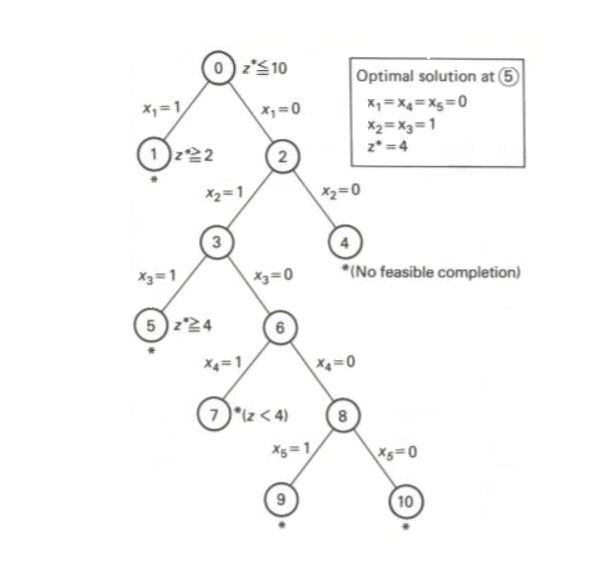
\includegraphics[width=200pt,height=200pt]{bnb_binary.eps}
%    \caption{Drvo odluke za rješavanje problema binarnog programiranja.}
%    \label{fig:bnb_binary1}
%\end{figure}

\begin{figure}
	\centering
\begin{tikzpicture}[
	node/.style={%
		draw,
		circle,
	},
	]
	% nacrtaj cvorove:
	\node [node, label={[blue]right:$z^* \leq 10$}] (A) { 0 };
	\path (A) ++(-135:\nodeDist) node [node, label={[blue]right:$z^* \geq 2$}] (B) {1};
	\path (A) ++(-45:\nodeDist) node [node] (C) {2};
	\path (C) ++(-135:\nodeDist) node [node] (D) {3};
	\path (C) ++(-45:\nodeDist) node [node, label={[blue]right:(Nema dopustivog rješenja)}] (E) {4};
	
	\path (D) ++(-135:\nodeDist) node [node, label={[blue]left:$z^* \geq 4$}] (F) {5};
	\path (D) ++(-45:\nodeDist) node [node] (G) {6};
	
	\path (G) ++(-135:\nodeDist) node [node, label={[blue]right:$z < 4$}] (H) {7};
	\path (G) ++(-45:\nodeDist) node [node] (I) {8};
	
	\path (I) ++(-135:\nodeDist) node [node, label={[blue]left: (Nije dopustivo)}] (K) {9};
	\path (I) ++(-45:\nodeDist) node [node, label={[blue]right: (Nije dopustivo)}] (L) {10};
	% nacrtaj grane:
	\draw (A) -- (B) node [left,pos=0.25] {$x_1=1$}(A);
	\draw (A) -- (C) node [right,pos=0.25] {$x_1=0$}(A);
	\draw (C) -- (D) node [left,pos=0.25] {$x_2=1$}(C);
	\draw (C) -- (E) node [right,pos=0.25] {$x_2=0$}(C);
	
	\draw (D) -- (F) node [left,pos=0.25] {$x_3=1$}(D);
	\draw (D) -- (G) node [right,pos=0.25] {$x_3=0$}(D);
	
    \draw (G) -- (H) node [left,pos=0.25] {$x_4=1$}(G);
	\draw (G) -- (I) node [right,pos=0.25] {$x_4=0$}(G);
	
    \draw (I) -- (K) node [left,pos=0.25] {$x_5=1$}(I);
	\draw (I) -- (L) node [right,pos=0.25] {$x_5=0$}(I);
	
	%add text (info) x1=x4=x5=0; x2=x3=1 je optimum:
	
\end{tikzpicture}
    \caption{Drvo odluke za rješavanje problema binarnog programiranja.}
    \label{fig:bnb_binary}
\end{figure}

Prodiskutujmo ovo rješenje po čvorovima dobijenog stabla:
  \begin{itemize}
      \item U čvoru 0 imamo  rješenje $x_i = 0$, za sve $i$, koje  nije dopustivo, ali  tada za optimalno rješenje vrijedi $z^*=f(x^*) \leq 10$.
      \item  Dalje, granamo ovaj problem na dva (korak 2), jedan gdje je $x_i=1$ a drugi $x_1=0$, odakle dobijamo dva podproblema (odgovaraju čvorovima 1 i 2). U čvoru 2 imamo podproblem za koji je $x_1=1$. Jasno je da kada uvrstimo $(1,0, \ldots, 0)$ u početni problem, da je ono dopustivo. Prema tome, optimalna vrijednost problema neće biti manji od 2, odakle zaključujemo da je za ovaj podproblem $z^*=f(x^*) \geq 2$. Dakle, imamo $LB$=2. 
      \item Problem u čvoru 2 je isti kao problem u čvoru 1, pa nastavljamo dalje sa dijeljenjem problema fiksirajući slobodne promjenljive. 
      \item Sada fiksiramo promjenjivu $x_2$ (uz već fiksiranu odluku $x_1=0$). 
            Za podproblem u čvoru 4, provjerimo da ne postoji dopuna do dopustivog rješenja za ovako fiksirane vrijednosti (narušeno ograničenje 1), čime se prekida dalje granjenje po ovoj grani. Za podproblem u čvoru 3, imamo sada podjelu na dva podproblema fiksiranjem promjenljive $x_3$, tj. dobijamo dva   nova čvora 5 i 6. Za problem u čvoru 5, lako se vidi da za ovakve fiksirane promjenljive imamo dopustivo rješenje za koje je vrijednost funkcije cilja jednaka 4, pa zaključujemo da je $z^*=f(x^*) \leq 4$, odakle imamo $LB=4$. Problem u čvoru 6 dijelimo dalje (po promjenljivoj $x_4$), odakle dobijamo dva nova podproblema, koji odgovaraju čvorovima 7 i 8. Lako se zaključi da je $z^*<LB$ za   podproblem u čvoru 7.  Za čvor 8, imamo novo grananje (po promjenljivoj $x_5$). Kako su ovdje sve promjenljive fiksirane, primijetimo da niti jedna od ovih tačaka  nije dopustiva.
            \item Prema tome, optimalno rješenje početnog problema je $LB=4$ i dostiže se u tački $x=(0, 1, 1, 0, 0)$. 
  \end{itemize}
  Totalna enumeracija bi generisala 32 čvora za gornji problem. Implicitna enumeracija generiše svega 11 čvorova. 
 
\section{Metoda odsjecajućih ravni}
  
\emph{Metoda odsjecajućih ravni} rješava problem cjelobrojnog  programiranja mijenjanjem rješenja njegove relaksacije, sve dok se ne dobije model čije je optimalno rješenje cjelobrojno. Metoda nije bazirana na principu dijeljenja dopustivog regiona problema na podregione, kao što je to slučaj sa B\&B metodama, već radi sa jednim linearnim programom, kojeg poboljšava iterativnim dodavanjem novih ograničenja. Nova ograničenja sukcesivno smanjuju dopustiv region, sve dok se ne pronađe cjelobrojno optimalno rješenje.   
 Istorijski gledano, to je prvi algoritam razvijen za probleme cjelobrojnog programiranja, za koji je formalno dokazano da konvergira ka optimumu u konačnom broju koraka. Iako se algoritam generalno smatra   neefikasnim, važan je sa metodološkog aspekta, jer je njegov razvoj kasnije doveo do konstrukcije drugih, efikasnijih algoritama.  
  
 \begin{definition}{Validna nejednakost} za ILP je svako ograničenje koje ne eliminiše niti   jedno  dopustivo cjelobrojno rješenje problema.
 \end{definition}
 Drugi naziv za \emph{validnu nejednakost} je \emph{odsjecajuća ravan}.

\begin{primjer}
Za sljedeći problem ILP-a
\end{primjer}
  \begin{align*}
    & \max z = 3x_1 + 4 x_2 \\
    & \mbox{t.d.} \\
    & 5x_1 + 8x_2\leq 24 \\
    & x_1, x_2 \geq 0, x_1,x_2\in \mathbb{Z},
 \end{align*}
jedna njegova validna nejednakost bi bila  $2z - x_1 = (6x_1 + 8x_1 ) - x_1 = 5x_1 + 8 x_2  \leq 24$, dakle $2z - x_1 \leq 24,$ a kako sigurno vrijedi $x_1 \leq 4$, dobijamo $2z \leq 24 + 5$. Iz prethodnog imamo $z \leq 14.5$, što zbog cjelobrojnosti funkcije cilja daje $z \leq 14$.


\begin{definition}
      Konveksni omotač za problem  ~(\ref{ilp-formulation}) je najmanji (dopustivi) poliedar nekog LP-a koji sadrži sve dopustive cjelobrojne tačke tog problema.
\end{definition}
Ako riješimo LP problem čiji je dopustivi skup konveksni omotač cjelobrojnih tačaka, onda je to rješenje optimalno za odgovarajući ILP. Međutim problem nalaska ovakvog konveksnog omotača je takođe  NP-težak, pa prema tome nije očekivano da se takav   omotač može naći u opštem slučaju. Nalazak korisnih ograničenja (ne svih) koja učestvuju u izgradnji konveksnog omotača je takođe veoma težak zadatak, mada je ovo ponekad i moguće. Prema tome, zadatak se svodi na nalazak korisnih odsjecajućih ravni, nezavisno od problema pronalaska konveksnog omotača, što se najčeše i radi  u praksi. 

\begin{primjer}
Posmatrajmo   \emph{problem pakovanja skupa} dat na sljedeći način. Neka je data kolekcija $D$ rombova (u $\mathbb{R}^2$). 
\end{primjer}
Zadatak je izabrati maksimalan broj rombova tako da se nikoja dva od njih ne presijecaju.  Za rombove kažemo da se presijecaju ako imaju barem jednu zajedničku tačku u presjeku. 
Neka je $O$ skup svih parova rombova koji se presijecaju. Sljedeći ILP odgovara ovom problemu:
\begin{align*}
    &\max \sum_{d\in D}x_d\\
    &\mbox{t.d.} \\
    & x_d + x_{d'} \leq 1, \forall (d, d^{'}) \in O \\
    & x_d \in \{0,1\}, \forall d \in D
\end{align*}
gdje je $x_d$ binarna promjenljiva, koja dobija vrijednost 1 ako je romb $d$ izabran u riješenju, inače 0. 
Kao što vidimo, broj binarnih promjenljivih u praksi može biti veoma velik, što otežava efikasnu primjenu neke od B\&B tehnika.

Pokušajmo dodati odsjecajuće ravni u prethodni ILP. Za svaku tačku $c$, enumerišimo sve one (moguće) rombove iz $D$ koji sadrže ovu tačku. Označimo takav skup sa $D(c)$. S obzirom na uslove zadatka, za svaki skup $D(c)$, najviše jedan romb može da bude odabran. Sada,  u prethodni model dodajemo sljedeća ograničenja
\begin{equation}
     \sum_{d \in D(c)} x_d \leq 1, \forall c.
\end{equation}
Ovim postupkom smo formirali odsjecajuće ravni, koje će ubrzati rješavanje posmatranog problema za   red veličine. \\

Razmotrimo sada \emph{Gomorijeve odsjecajuće ravni}, kao generalnu metodu za dodavanje odsjecajućih ravni u rješavanju  ILP-a.  Ideja se sastoji u generisanju ravni iz nekog od ograničenja dobijenim optimalnom tabelom simpleks metode, koja predstavlja LP relaksaciju problema. Neka simpleks metod generiše sljedeći skup jednakosti u formi:
 

$$x_i + \sum_{ j} \overline{a}_{i,j} s_j= \overline{b}_i, i=1, \ldots,m$$
gdje su $x_i$ bazne promjenjive, $s_j$ nebazne promjenjive, dok su vrijednosti $\overline{a}_{ij}$ elementi gornje lijeve podmatrice optimalne simpleks tabele~(\ref{tab:simplex_tabelau}) koji odgovaraju baznim vektorima.  
 
 Napišimo prethodnu jednakost u drugačijem obliku tako da se na lijevoj strani nalaze cjelobrojni dijelovi, dok su na desnoj decimalni dijelovi, tj.
$$x_i + \sum_{j} \lfloor \overline{a}_{i,j} \rfloor s_j - \lfloor \overline{b}_i \rfloor = \overline{b}_i - \lfloor \overline{b}_i  \rfloor    - \sum_{j} (\overline{a}_{i,j} - \lfloor \overline{a}_{i,j} \rfloor) s_j.$$

Ako je $x$ dopustivo cjelobrojno rješenje, onda je desna strana manja od 1, a kako je lijeva strana cjelobrojna u tom slučaju, dobijamo da je desna strana manja ili jednaka 0, pa imamo
\begin{equation}\label{eq:gomory_cuts}
    \overline{b}_i - \lfloor \overline{b}_i  \rfloor    - \sum_{j} (\overline{a}_{i,j} - \lfloor \overline{a}_{i,j} \rfloor) s_j \leq 0
\end{equation}
za bilo koje (bazno) dopustivo rješenje $x$ koje je cjelobrojno. Dalje, kako su vrijednosti nebaznih promjenjivih jednake 0 u bilo kom baznom dopustivom rješenju, zaključujemo
$$ \overline{b}_i - \lfloor \overline{b}_i  \rfloor    - \sum_{ij} (\overline{a}_{i,j} - \lfloor \overline{a}_{i,j} \rfloor) s_j = \overline{b}_i - \lfloor \overline{b}_i \rfloor  \geq 0.$$
Prema tome, pokazali smo da odsjecajuće ravni~(\ref{eq:gomory_cuts}) ne eliminišu bazna dopustiva rješenja, pa ispunjavaju sve uslove za validnu nejednakost. Uvodeći dodatnu promjenjivu $y_i$ za nejednakosti u (\ref{eq:gomory_cuts}), sljedeća (validna) ograničenja dodajemo u ILP:
\begin{align}\label{gomory_cplex}
       \overline{b}_i - \lfloor \overline{b}_i \rfloor=   \sum_{j} (\overline{a}_{i,j} - \lfloor \overline{a}_{i,j} \rfloor)s_j - y_i 
\end{align}

\begin{primjer} Neka je dat sljedeći problem ILP-a
	\end{primjer}
\begin{align*}
    &\max\ 3 x_1 + 4 x_2 \\
    & \mbox{t.d. }  \\
    & \displaystyle\frac{2}{5}x_1 + x_2 \leq 3 \\
    & \displaystyle\frac{2}{5}x_1 - \frac{2}{5}x_2 \leq 1 \\
    &x_1, x_2 \geq 0, \\
    &  x_1, x_1 \in \mathbb{Z}.
\end{align*}
Riješimo ga uz pomoć Gomorijevih odsjecajućih ravni. 

\emph{Rješenje.}
Inicijalna simpleks tabela (LP relaksacije) je data sa 

$$\begin{array}{cccc|c}\vspace{1mm}
   \frac{2}{5}           & 1               & 1 & 0 & 3 \\\vspace{1mm}
   \frac{2}{5}           & -\frac{2}{5}    & 0 & 1 & 1 \\ \hline
   -3                    &  -4             & 0 & 0 & 0
\end{array}$$
Uključimo drugu promjenljivu (odg. kolona 2) u bazu, pa imamo 
$$\begin{array}{cccc|c}\vspace{1mm}
   \frac{2}{5}           & 1               & 1           & 0 & 3 \\\vspace{1mm}
   \frac{14}{25}         & 0    & \frac{2}{5} & 1&\frac{11}{5}\\\hline\vspace{1mm}
   -\frac{7}{5}     & 0     &4 & 0 & 12
\end{array}$$
Dalje, biramo novi pivot  u prethodnoj simpleks tabeli, a to je element $\overline{a}_{2,1} = \frac{14}{25}$, pa transformacijama dobijamo simpleks tabelu
$$
\begin{array}{cccc|c}\vspace{1mm}
    0    &  1  &  \frac{10}{14} &  -\frac{10}{14}  &  \frac{20}{14}  \\\vspace{1mm}
    1    &  0  &  \frac{10}{14} &   \frac{25}{14}  &   \frac{55}{14}\\ \hline
    0    &  0  &  5             &    \frac{5}{2}   &    \frac{35}{2}
\end{array}
$$
Kako u posljednjoj vrsti nemamo negativnih vrijednosti, zaključujemo da je ovo optimalna simpleks tabela. Na osnovu (\ref{gomory_cplex}),   za prvi red simpleks tabele i odgovarajuće ogranjičenje generišemo odsjecajuću ravan:
$$   \frac{5}{7}s_1 + \frac{2}{7} s_2 -      y_1   = \frac{6}{14}=\frac{3}{7}$$
pa je dodajemo u (završnu) simpleks tabelu:
$$
\begin{array}{ccccc|c}\vspace{1mm}
    0    &  1  &  \frac{10}{14} &  -\frac{10}{14}  &  0 & \frac{20}{14} \\\vspace{1mm}
    1    &  0  &  \frac{10}{14} &   \frac{25}{14}  &  0 & \frac{55}{14}\\ \vspace{1mm}
    0    &  0  & \frac{5}{7}    &   \frac{2}{7}    &  -1 & \frac{3}{7}  \\\hline \vspace{1mm}
    0    &  0  &  5             &    \frac{5}{2}   &  0 &    \frac{35}{2}
\end{array}
$$
Formirajmo sada jediničnu podmatricu u gornjoj lijevoj matrici $\overline{A}$, imajući u vidu treću kolonu (i odgovarajuću promjenljivu $s_1$), a pivotirajući oko elementa $\overline{a}_{3,3}$. Dobijamo 

$$
\begin{array}{ccccc|c}
    0    &  1  &   0 &   -1  &            1 & 1                  \\
    1    &  0  &  0 &    \frac{3}{2}  &  1 & \frac{7}{2}\\ \vspace{1mm}
    0    &  0  &  1  &   \frac{2}{5}    &  -\frac{7}{5} & \frac{3}{5}  \\ \hline \vspace{1mm}
    0    &  0  &  0   &    \frac{1}{2}  &  7  &    \frac{29}{2}
.\end{array}
$$
Kao što vidimo, rješenje problema je $(\frac{7}{2}, 1, 0, 0, \frac{3}{5})$, što i dalje nije cjelobrojno rješenje. Dalje, dodajemo novu odsjecajuću ravan, koja se izvodi iz drugog ograničenja (drugi red simpleks tabele).
$$ \frac{1}{2} s_2 - y_2 = \frac{1}{2}.$$
Dodajmo ovo ograničenje u posljednju simpleks tabelu

$$
\begin{array}{cccccc|c}\vspace{1mm}
    0    &  1  &   0 &   -1  &            1 & 0 & 1                  \\\vspace{1mm}
    1    &  0  &  0 &    \frac{3}{2}    &  1 & 0 &  \frac{7}{2}\\ \vspace{1mm}
    0    &  0  &  1  &   \frac{2}{5}    &  -\frac{7}{5} &  0 & \frac{3}{5}  \\\vspace{1mm}
    0    & 0   &  0  &   \frac{1}{2}    & 0     & -1 & \frac{1}{2} \\ \hline\vspace{1mm} 
    0    &  0  &  0   &    \frac{1}{2}  &  7  &   0 &  \frac{29}{2}
\end{array}
$$
Sada za promjenljivu $x_4$ (četvrta kolona), pivotiramo oko elementa $\overline{a}_{4,4}$, pa dobijamo simpleks tabelu 

$$
\begin{array}{cccccc|c}
0 &  1   &  0  &  0  &    1             &    -2           &   2         \\
1 &  0   &  0  &  0  &    1             &     3           &   2         \\
0 &  0   &  1  &  0  &   -\frac{7}{5}   &     \frac{4}{5} &   \frac{1}{5}\\
0 &  0   &  0  &  1  &   0              &    -2           &   1   \\ \hline
0 &  0   &  0  &  0  &   7              &     1           &   14
\end{array}
$$


Iz tabele zaključujemo da je bazno rješenje problema 
$x=(2,2, \frac{1}{5}, 1)$, a optimalno $x^* = (2, 2)$, odakle dobijamo i optimalno rješenje početnog problema. 


%https://www.math10.com/en/geometry/geogebra/geogebra.html
\begin{primjer}  U ovom primjeru ćemo prikazati ILP problem u kojem su svi koeficijenti u ograničenjima cjelobrojni.
	\end{primjer}
\begin{align*}
    &\max 3 x_1 + 4 x_2 \\
    &\mbox{t.d.} \\
    & 3 x_1 - x_2 \leq 12 \\
    & 3 x_1 + 11 x_2 \leq 66 \\
    & x_1, x_2 \geq 0 \\
    & x_1, x_2 \in \mathbb{Z}
\end{align*}
\emph{Rješenje. }
 Na Slici~ \ref{fig:region_ilp_primjer_2} dat je skup tačaka koje su dopustive za problem. Funkcija cilja dostiže optimum u tački $x^*=(5,4)$.
 \begin{figure}
    \centering
    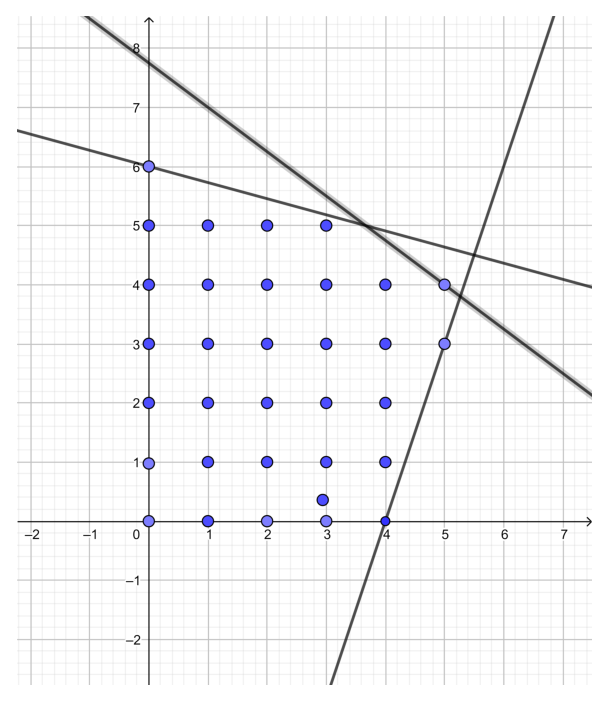
\includegraphics[width=170pt,height=170pt]{region_ilp_primjer_2.eps}
    \caption{Dopustiv skup tačaka problema.}
    \label{fig:region_ilp_primjer_2}
\end{figure}

Riješimo sada ovaj problem uz pomoć Gomorijevih odsjecajućih ravni. 
Početna simpleks tabela je data sa 
$$\begin{array}{ccc c| c}
    3  & -1 & 1 &  0  & 12  \\
    3  & 11 & 0 &  1  & 66 \\ \hline
   -3  & -4 & 0 &  0  & 0
\end{array}$$
Nakon dvije iteracije pivotiranja, dobijamo simpleks tabelu 
$$\begin{array}{ccc c| c}\vspace{1mm}
1 & 0 &  \frac{11}{36}   &  \frac{1}{36}  &  \frac{11}{2} \\\vspace{1mm}
0 & 1 &  -\frac{1}{12}  &  \frac{1}{12}  &  \frac{9}{2}   \\ \hline\vspace{1mm}
0 & 0 &  \frac{7}{12}   &  \frac{5}{12}  &  \frac{69}{2}
\end{array} $$
Optimalno rješenje je $x = (\frac{11}{2}, \frac{9}{2}, 0, 0)$ koje nije cjelobrojno. Dodajmo Gomorijevu odsjecajuću ravan generisanu iz ograničenja prve vrste simpleks tabele (za prvu baznu komponentu $x_1 = \frac{11}{2}$):
$$  \frac{11}{36} x_2 + \frac{1}{36} s_1 - y_1 = \frac{1}{2},$$
pa dobijamo tabelu 
$$\begin{array}{ccccc| c}\vspace{1mm}
1 &  0 &   \frac{11}{36}  & \frac{1}{36}   &  0 & \frac{11}{2} \\\vspace{1mm}
0 &  1 &   -\frac{1}{12}  & \frac{1}{12}   &  0 & \frac{9}{2} \\\vspace{1mm}
0 &  0 &  \frac{11}{36}   &  \frac{1}{36}  & -1 & \frac{1}{2} \\ \hline\vspace{1mm}
0 & 0  &  \frac{7}{12}    & \frac{5}{12}   &  0 & \frac{69}{2}
\end{array} $$
Kako bazno dopustivo rješenje nije očigledno, primijenimo dvofazni simpleks metod da bi izabrali bazu. Dobijamo tabelu
$$\begin{array}{ccccc| c}
1   &   0       &   0   &   0             & 1              & 5 \\
0   &   1       &   0   &   \frac{1}{11}  & -\frac{3}{11}  & \frac{51}{11} \\
0   &   0       &   1   &   \frac{1}{11}  & -\frac{36}{11} &  \frac{18}{11} \\ \hline
0   &   0       &   0   &   \frac{4}{11}  & \frac{21}{11}  &  \frac{369}{11} \\
\end{array} $$
Kako su svi koeficijenti u posljednjoj vrsti veći od 0, slijedi da je optimalno bazno rješenje jednako $x=(5, \frac{51}{11}, \frac{18}{11}, 0, 0)$, koje opet nije cjelobrojno. 
 Prema tome, dodajmo sljedeću Gomorijevu odsjecajuću ravan za bazno rješenje $x_2 = \frac{51}{11}$ (posmatrajući vrstu 2 posljednje simpleks tabele):
 
 $$ \frac{1}{11} s_2 + \frac{8}{11} y_1 - y_2 = \frac{7}{11},$$
 odakle imamo tabelu 
 $$\begin{array}{cccccc| c}
 1   &   0   &  0  &   0             &   1  &   0              &   5 \\\vspace{1mm}
 0   &   1   &  0  &  \frac{1}{11}    &   -\frac{3}{11}    &  0 & \frac{51}{11} \\\vspace{1mm}
 0   &   0   &  1  &  \frac{1}{11}    & -\frac{36}{11}       & 0 & \frac{18}{11}  \\\vspace{1mm}
 0   &   0   &  0  &  \frac{1}{11}    &  \frac{8}{11}   & -1 & \frac{7}{11} \\ \hline\vspace{1mm}
 0   &   0   &  0  &   \frac{4}{11}   &   \frac{21}{11} & 0 & \frac{369}{11}
\end{array} $$
I ovdje nije očigledno šta su bazne promjenljive, pa i ovdje primijenimo dvofazni simpleks metod. Nakon toga, dobijamo 
 $$\begin{array}{cccccc| c}
1    &   0   &   0   &  -\frac{1}{8}   &   0    &    \frac{11}{8}    &  \frac{33}{8} \\\vspace{1mm}
0    &   1   &   0   &   \frac{1}{8}   &   0    &    -\frac{3}{8}    & \frac{39}{8} \\\vspace{1mm}
0    &   0   &   1   &   \frac{1}{2}   &   0    &    - \frac{9}{2}   & \frac{9}{2} \\\vspace{1mm}
0    &   0   &   0   &   \frac{1}{8}   &   1    &    - \frac{11}{8}  & \frac{7}{8} \\ \hline\vspace{1mm}
0    &   0   &   0   &   \frac{1}{8}   &   0    &     \frac{21}{8}   & \frac{255}{8}
\end{array} $$
Odgovarajuće optimalno bazno dopustivo rješenje i dalje nije cjelobrojno -- niti jedna komponenta nije cjelobrojna. 

Prema tome, dodajemo novu Gomorijevu odsjecajuću ravan za vrstu 2 prethodne simpleks tabele, koja je oblika
$$  \frac{1}{8}s_2 + \frac{5}{8} y_2 - y_3 = \frac{7}{8},$$
te dobijamo tabelu
$$ \begin{array}{ccccccc| c}\vspace{1mm}
1    &   0   &   0   &  -\frac{1}{8}   &   0    &    \frac{11}{8}    & 0 & \frac{33}{8} \\\vspace{1mm}
0    &   1   &   0   &   \frac{1}{8}   &   0    &    -\frac{3}{8}    & 0 & \frac{39}{8} \\\vspace{1mm}
0    &   0   &   1   &   \frac{1}{2}   &   0    &    - \frac{9}{2}   & 0 & \frac{9}{2} \\\vspace{1mm}
0    &   0   &   0   &   \frac{1}{8}   &   1    &    - \frac{11}{8}  & 0    & \frac{7}{8} \\ \vspace{1mm}
0    &   0   &   0   &   \frac{1}{8}   &   0    &    \frac{5}{8}     & -1 & \frac{7}{8} \\ \hline\vspace{1mm}
0    &   0   &   0   &   \frac{1}{8}   &   0    &     \frac{21}{8}   & 0 & \frac{255}{8}   
\end{array} $$
I ovdje nije očigledno koju   promjenljivu treba dodati u bazne promjenljive (bazu), pa primijenimo dvofazni simpleks metod, odakle dobijamo 

$$ \begin{array}{ccccccc| c}\vspace{1mm}
    1    &   0   &   0   &  0 &  1  &   0    &    0    & 5  \\\vspace{1mm}
0    &   1   &   0   &  0   &   -\frac{1}{2}    &   0   & \frac{1}{2} & 4 \\\vspace{1mm}
0    &   0   &   1   &  0   &   -\frac{7}{2}    &   0   & \frac{1}{2} & 1 \\\vspace{1mm}
0    &   0   &   0   &  1  &   \frac{5}{2}    &  0 &  -\frac{11}{2}    & 7 \\ \vspace{1mm}
0    &   0   &   0   &   0 &  -\frac{1}{2}    &   1   & - \frac{1}{2} & 0\\ \hline\vspace{1mm}
0    &   0   &   0   &  0  &   1    &    0   & 2 & 31  
\end{array} 
$$
gdje je lako uočiti da je optimalno bazno dopustivo rješenje $x=(5, 4, 1, 7, 0, 0, 0 )$, tj. rješenje početnog problema je $x^*=(5, 4)$.

\section{B\&C algoritam za rješavanje ILP-a}
%https://homepages.rpi.edu/~mitchj/handouts/bc_algo/
% http://www.mi.fu-berlin.de/wiki/pub/Main/GunnarKlauP1winter0708/discMath_klau_ILP_I.pdf
U ovom odjeljku analiziramo metodu granjanja i odsijecanja (eng. branch and cut, skraćeno B\&C). U odnosu na B\&B metodu, koja je opisana u Odjeljku~\ref{sec:bb}, B\&C dodaje  i metod odsjecajućih ravni u rješavanju  podproblema koji odgovaraju čvorovima drveta. Dakle, ako  uzimamo trenutno aktivni čvor i rješavamo odgovarajući podproblem, dijelimo ga na nekoliko podproblema (podjelom dopustivog regiona na više disjunktnih -- dodavanjem ograničenja) ili ga rješavamo rekurzivnim dodavanjem (Gomorijevih) odsjecajućih ravni. Ilustrujmo ovu ideju na primjeru rješavanja jednog ILP-a.
\begin{primjer} 
	Riješimo sljedeći ILP
\end{primjer}
\begin{align*}
    &\max 6 x_1 + 5 x_2 \\
    &  \mbox{t.d. } \\
    & 3x_1 + x_2 \leq 11 \\
    & - x_2 + 2 x_2 \leq 5 \\
    & x_1, x_2 \geq 0 \\
    & x_1, x_1 \in \mathbb{Z}
\end{align*}

\emph{Rješenje}. B\&C procedura prvo rješava LP relaksaciju početnog problema (simpleks metodom), odakle dobijamo rješenje $x=(\frac{17}{7}, \frac{26}{7})$
sa optimalnom vrijednošću $33\frac{1}{7}$. Nakon toga treba da se donese odluka, da li se problem rješava dodavanjem odsjecajućih ravni ili podjelom dopustivog regiona na manje (disjunktne) podregione. Podijelimo region po koordinati $x_1$, odakle ćemo dobiti dva podproblema 
\begin{align*}
    &\max 6 x_1 + 5 x_2 \\
     &  \mbox{t.d. } \\
    & 3x_1 + x_2 \leq 11 \\
    & - x_2 + 2 x_2 \leq 5 \hspace{2cm} (P1) \\
    & x_1 \geq 3 \\
    & x_2 \geq 0 \\
    & x_1, x_2 \in \mathbb{Z}
\end{align*}

\begin{align*}
    &\max 6 x_1 + 5 x_2 \\
      &  \mbox{t.d. } \\
    & 3x_1 + x_2 \leq 11 \\
    & - x_2 + 2 x_2 \leq 5 \hspace{2cm} (P2) \\
    & x_1  \leq 2 \\
    & x_2 \geq 0 \\
    & x_1, x_2 \in \mathbb{Z}
\end{align*}

Rješavanjem relaksacije problema ($P1$) dobijamo rješenje $x^*=(3,2)$, koje je cjelobrojno, pa prema tome i dopustivo u početnom problemu. Vrijednost funkcije cilja je 28, što je i donja granica ($LB$) početnog problema. Relaksacija problema ($P2$) nam daje rješenje $x^*=(2, \frac{7}{2})$, čija je optimalna vrijednost $29.5$.  Prema tome, rješenje nije cjelobrojno. Primjenjujući metod Gomorijevih odsjecajućih ravni na problem ($P2$), konstruišemo odsjecajuću ravan $2x_1 + x_2 \leq 7$ koju dodajemo u problem ($P2$), pa dobijamo problem 
\begin{align*}
    &\max 6 x_1 + 5 x_2 \\
    & \mbox{t.d. } \\
    & 3x_1 + x_2 \leq 11 \\
    & - x_2 + 2 x_2 \leq 5  \\
    & 2x_1 + x_2 \leq 7 \hspace{2cm} (P3)\\ 
    & x_1  \leq 2 \\
    & x_2 \geq 0 \\
    & x_1, x_2 \in \mathbb{Z}
\end{align*}

Rješavajući LP relaksaciju problema ($P3$), dobijamo rješenje $x^*=(\frac{9}{5}, \frac{17}{5})$, a  optimalna vrijednost funkcije cilja je $27.8$. Kako je $LB \geq 27.8$, niti jedno cjelobrojno rješenje problema ($P3$) ne može biti bolje od trenutno najbolje donje granice ($LB=28$), pa zaključujemo da je optimalo rješenje početnog problema dato sa $x^*=(3,2)$. 

\section{Lagranžova relaksacija}
U rješavanju problema optimizacije, pronalazak optimalnog rješenja je osnovni cilj. Međutim, za mnoge probleme nije realno očekivati da će se razumnom vremenu može doći do optimalnog rješenja za instance velikih dimenzija. Umjesto toga, najbolje što se može učiniti je da se ponudi dobra  granica za optimalnu vrijednost. Ako je ta granica blizu optimuma, u mnogo slučajeva ona može da zamijeni optimum, čime štedimo resurse kojima raspolažemo, a dobijamo rješenje koje je prihvatljivo.  

Ideja \emph{Lagranžove relaksacije} se sastoji u tome da u modelu ILP-a  koji ima  ograničenja koja problem čine teškim (ova procjena najčešće dolazi uz praktičnog iskustva),  posmatramo kao dio ciljne funkcije koji se penalizuje nekim parametrom.  %parametrom $\lambda>0$. 
Ovo ograničenje potom brišemo iz skupa ograničenja modela, a zatim rješavamo ovakav (parametrizovan) problem. Fiksirajući parametar penalizacije, rješenje takvog problema predstavlja donju granicu (za problem minimizacije)  optimalnog rješenja inicijalnog problema. Dobijena granica je često dovoljno blizu vrijednosti optimuma, što ovu metodu čini upotrebljivom u rješavanju praktičnih problema. 

\begin{primjer} Posmatrajmo problem \emph{najkraćeg puta sa ograničenjem} (eng.  {Constrained shortest path problem}). Neka je dat usmjeren neciklični graf $G=(V,E)$. Za svaku granu $(i,j) \in E$ dodijelimo cijenu puta $c_{i,j}$ i vrijeme putovanja $t_{i,j}$. Pretpostavimo da je čvor $i=1$ početni (izvorni) čvor, a čvor $n = |V|$   završni čvor (terminalni čvor). Zadatak je da se nađe najjeftiniji put  od izvornog do terminalnog čvora, ali tako da se čitav put pređe u vremenskom periodu $T$.
\end{primjer}
Ovaj problem se modeluje pomoću sljedećeg ILP-a:
 \begin{align}
    &z^*=\min\sum_{(i,j) \in E }c_{i,j}x_{i,j} \\
    &\mbox{t.d. }\\
    & \sum_{i} x_{i,j} - \sum_{i} x_{j,i} = \begin{cases}  
                                               1, \mbox{ ako } i=1 \\
                                              -1, \mbox{ ako } i=n \\
                                               0, \mbox{ inače }
                                            \end{cases},  \forall j \in V \\ 
    & \sum_{(i,j) \in E} t_{i,j} x_{i,j} \leq T, \forall j \in V \\
    & x_{i,j} \in \{0, 1 \}, \forall (i,j) \in E.
\end{align} 

Binarna promjenljiva $x_{i,j}$ dobija vrijednost 1 ako je  na   putu odabrana grana $(i,j)$, a 0 inače. 
Prvo ograničenje u modelu osigurava da je dopustivo rješenje upravo put od izvornog do terminalnog čvora. Drugo ograničenje nam modeluje uslov da vrijeme prelaska puta treba da bude u  granicama dopustivog. Ova ograničenja spadaju u ,,teška'', jer se njihovim dodavanjem u model, njegovo rješavanje značajno otežava (vrijeme potrebno za rješavanje se drastično povećava i/ili  kompleksnost problema se teorijski povećava -- npr. sa P na NP). Kao što znamo,  pronalazak najkraćeg puta u usmjerenim grafovima, sa unaprijed definisanim izvornim čvorom, je polinomijalno rješiv (na primjer, uz pomoć Dajkstrinog algoritma). Međutim,  dodavanjem ograničenja u vezi vremena, taj problem postaje NP-težak. Stoga, ideja je  relaksirati ovaj problem uz prebacivanje ograničenja za vrijeme u funkciju cilja, koja se zatim kažnjava penalom. 
Dakle, Lagranžova relaksacija problema je data sa

\begin{align*}
       &L(\lambda)= \min\sum_{(i,j) \in E }c_{i,j}x_{i,j}  + \lambda(\sum_{(i,j) \in E} t_{i,j} x_{i,j} - T ) = \min \sum_{(i,j) \in E} (c_{i,j} + t_{i,j} )x_{i,j} - \lambda T \\
        &{\mbox{t.d.} }\\
    & \sum_{i} x_{i,j} - \sum_{i} x_{j,i} = \begin{cases}  
                                               1, \mbox{ ako } i=1 \\
                                              -1, \mbox{ ako } i=n \\
                                               0, \mbox{ inače},
                                            \end{cases} \forall j \in V\\
     & x_{i,j} \in \{0, 1 \}, \forall (i,j) \in E.
\end{align*}
Primijetimo da je $L(\lambda) \leq z(\lambda)  \leq z^*$, za sve $\lambda > 0$, gdje je $z(\lambda)$ problem koji ima funkciju cilja $L(\lambda)$ uz uključeno ograničenje o vremenu u skup ograničenja modela. Dakle, za $\lambda >0$, $L(\lambda)$ nam daje donju granicu za optimalno rješenje početnog problema. 

Problem $L^* = \max \{ L(\lambda) \mid \lambda > 0  \}$ se naziva \emph{problem Lagranžovog množioca}. Može se pokazati da vrijedi 
$$ L(\lambda) \leq L^* \leq z^*.$$

U praksi se pokazalo da je Lagranžova relaksacija dobra tehnika za dobijanje granica optimalne vrijednosti problema. 
 
\begin{primjer}
Primijenimo ovu tehniku na \emph{problem trgovačkog putnika} sa ulaznim težinskim grafom $G=(V,E)$, gdje je $V=\{1, \ldots, n\}$.  Razmotrimo  problem sa grafovske strane i pokušajmo da izvedemo njegovu relaksaciju. %Neka je data kolekcija grana $T. Kolekcija grana $T$ formira konturu ako su svaka dva čvora grafa $G$ pokrivena sa tačno dvije grane iz te kolekcije. Kada obrišemo grane incidentne sa čvorom 1 (ili nekim drugim), ostatak rute će činiti stablo koje pokriva graf  $G\setminus \{1\}$.  
% Definišimo sa $A(j)$ skup svih čvorova koji su incidentni sa čvorom $j$. 
\end{primjer}
Relaksacija: definišimo sa $T_1$ skup svih ruta  u $G$  koje nakon brisanja grana koje pokrivaju čvor $1$ formiraju (pokrivajuće) stablo.  Dakle, prije samog rješavanja problema, enumerišimo sve ovakve rute u grafu $G$. 

Shodno tome, konstruišemo sljedeći model
\begin{align*}
    &z^* = \min \sum_{(i,j)\in E} c_{i,j} x_{i,j}\\
    & \mbox{t.d.} \\
    & \sum_{ \{ i \mid (i,j) \in E \} } x_{i,j} = 2, \forall i \in \{1,\ldots, n \} \\
    & x \in T_1,
\end{align*}
gdje $x_{i,j} = 1$ ako grana $(i,j)$ pripada ruti, a 0 inače. Ako je $x=(i, j) \in T_1$, to znači da postoji neka ruta u $G$ u kojoj su čvorovi $i$ i $j$ susjedni, gdje se nakon brisanja grana čvora $1$, formira (pokrivajuće) stablo grafa $G$. 

Lagranžova relaksacija za ovaj problem može se zadati sa 
\begin{align*}
     &L(\lambda) = \min \sum_{(i,j)\in E} c^\lambda_{i,j} x_{i,j} - 2 \sum_{i} \lambda_i \label{eq:tsp-lagrangean}\\
     & x \in T_1
\end{align*}
gdje je $\lambda=(\lambda_1, \ldots, \lambda_n)$ i $c^\lambda_{i,j} = c_{i,j} + \lambda_i + \lambda_j$. 

U praksi se pokazalo da su rješenja dobijena Lagranžovom relaksacijom blizu optimalnim rješenju problema. Optimalno pokrivajuće stablo Lagranžovog problema $L(\lambda^*)$ za optimalno $\lambda^*$ će nam,  u praksi, često dati rješenje sa  nekoliko visećih čvorova. 

Konstruišimo još jednu Lagranžovu relaksaciju za ovaj problem,  uvodeći tzv. \emph{ograničenja pokrivanja}. Neka je dat skup $S\subseteq V$. Ograničenje pokrivanja u odnosu na skup $S$ osiguravaju postojanje najviše $|S|-1$ grana u svakoj ruti kojima oba kraja pripadaju čvorovima iz $S$. Ovom smo ograničili pojavljivanje ciklusa među čvorovima u konačnom rješenju.
Prethodni scenario modelujemo sljedećim modelom 
\begin{align*}
     & z^* = \min \sum_{(i,j)\in E} c_{i,j} x_{i,j} \\
     & \mbox{t.d.} \\
     & \sum_{ \{ i \mid (i,j) \in E \} } x_{i,j} = 2, \forall i \in \{1,\ldots, n \} \\
     & \sum_{(i,j) \in E \ \wedge\ i,j \in S} x_{i,j} \leq |S|-1, \forall S \subseteq V  \\
     &   \sum_{(i,j) \in E} x_{i,j} = n  \\
     & x_{i,j} \in \{0, 1 \}, (i,j)\in E.
\end{align*}
Lagranžova relaksacija prethodnog ILP-a ima oblik 
\begin{align*}
 &L(\lambda) = \min \sum_{(i,j)\in E} c^\lambda_{i,j} x_{i,j} - 2 \sum_{i} \lambda_i \\
 & \mbox{t.d.} \\
 & \sum_{(i,j) \in E} x_{i,j} \leq |S|-1, \forall S \in V \\
 & \sum_{(i,j) \in E} x_{i,j} = n
\end{align*}
gdje je $\lambda=(\lambda_1, \ldots, \lambda_n)$ i $c^\lambda_{i,j} = c_{i,j} + \lambda_i + \lambda_j$. 

% interior point method (dodati)...
\section{Metod generisanja kolona}% ovo je za LP probleme sa velikim brojem kolona, pogledati u https://coral.ise.lehigh.edu/~ted/files/ie418/lectures/Lecture18.pdf file:///C:/Users/PC/Downloads/ColumnGenerationTutorial.pdf

%video: https://www.youtube.com/watch?v=O918V86Grhc
U praksi se često nailazi  na situaciju da je u LP-u (ili ILP-u) broj promjenljivih značajno (eksponencijalno) veći  u odnosu na broj ograničenja. Kod takvih ekstremno velikih modela, matrica modela je izuzetno velikih dimenzija. Sa druge strane, veliki dio matrice (tj. njene kolone) nam obično nikada i neće biti relevantan za rješavanje. Da bi se riješila specifična instanca problema, ono što nam je potrebno su:
\begin{itemize}
    \item Ograničenja koja se vezuju uz optimalnost.
    \item Promjenljive koje su bazne u optimalnom rješenju.
\end{itemize}
Dakle, ono što je potrebno da znamo su ograničenja, čije su odgovarajuće dualne vrijednosti pozitivne, kao i promjenljive koje imaju pozitivne vrijednosti koeficijenata doprinosa za optimalno rješenje (tj. vektor  $\overline{c}$ iz simpleks tabele). Ako bismo  ove promjeljive i ograničenja imali na raspolaganju od samog početka, problem bi bio riješen efikasno. Međutim, do ove informacije nije jednostavno doći.  U simpleks metodi, vektor doprinosa je potrebno računati u svakoj iteraciji, što nije efikasno ako je matrica $A$ velikih dimenzija. Takođe, vrijeme potrebno za generisanje simpleks tabele bi bilo ogromno.  Oba ova problema su rješiva uz pomoć \emph{metode generisanja kolona}.  Ideja ovog metoda se sastoji u sljedećem. 
 

\begin{itemize}
   % \item ¸Krenimo sa ,,obećavajućim'' podskupom $S$ kolona matrice $A$; 
   \item Izaberimo podskup $S$ kolona matrice $A$ u cilju određivanja potencijalno dobrog inicijalnog baznog dopustivog rješenja
    \item Riješimo restrikovani LP na podskupu kolona $S$.
    \item Procijenimo ostale kolone i dodajmo u $S$ one sa negativnim 
          cijenama doprinosa.
    \item Iterativno pozivamo perthodna dva koraka dok god postoje kolone   sa negativnim doprinosom koje nisu u $S$.
\end{itemize}
Tehnički zapisano, krećemo od \emph{restrikovanog master problema} (RMP)
\begin{align*}
    &\min c^T x \\
    &\mbox{t.d} \\
    & \sum_{i \in I} A_i x_i  \leq b \hspace{2cm} (RMP)\\
    & x \geq 0. 
\end{align*}
gdje $I$ inicijalizujemo kao skup kolona koje čine inicijalno bazno dopustivo rješenje  za RMP. Po mogućnosti, dodajemo i neke druge kolone za koje smatramo da su ,,bitne'' u kontekstu problema.  Riješimo RMP,  te izračunamo odgovarajuće optimalno dualno rješenje. Sada je potrebno naći promjenljivu $x_j$ i odgovarajuću kolonu $A_j$ za koju je koeficijent doprinosa negativan, tj. $\overline{c_j} = c_j - c_B^T B^{-1}A_j < 0$.
%Pogledati: https://www.youtube.com/watch?v=0SV99VJaGzw
Ovo se može uraditi rješavanjem tzv. podproblema generisanog kolonama (eng. \emph{column generating subproblem -- CGSP}):
$$\min_{a \in C} \overline{c_j} = \min_{a \in C} c_a - c_B^T B^{-1} a,$$
gdje je $C$ skup kolona nad nekim globalnim skupom. Za LP problem možemo staviti $C = \{1,\ldots,n\}$. 

Ako je rješenje problema kolona $a \in C$ za koju je $\overline{c_a}<0$, dodamo odgovarajuću vektor kolonu $A_a$ u skup $S$, te riješimo  RMP na novom skupu kolona. Ako ne postoji takva kolona, onda je rješenje RMP takođe optimalno i za početni problem. %Ovaj metod se još naziva \emph{generički metod generisanja kolona}.   
 Proces dodavanja kolona se nastavlja sve dok postoji kolona $a\in C$ sa negativnom cijenom doprinosa. 

Postoji više različitih pristupa koje se odnose na ažuriranje skupa $S$ tokom iteracija. 
Najjednostavniji pristup je zadržavanje svake kolone koja je do sada izgenerisana  u skup $S$ i dodavanje  nove u postojeći skup. Naprednija strategija je zasnovana na izbacivanju onih kolona iz skupa $S$ koje su nebazne u svakoj iteraciji. 

\emph{Bazna šema za generisanje kolona}. U osnovi, šema se sastoji od dva koraka:
\begin{enumerate}
	\item  Za ulazne kolone prvo izaberemo one sa najvećim negativnim koeficijentom doprinosa, među promjenljivima koje odgovaraju skupu $I$.
	\item Jednom kada su svi koeficijenti nenegativni (tj. kada smo našli optimalnu vrijednost za  RMP), tražimo nove promjenljive (kolone) van skupa $I$ (rješavajući CGSP), koje će biti ubačene u $I$. 
\end{enumerate}
Ako u koraku 1 za skup $I$ uzmemo bazne kolone, u svakom koraku pri rješavanju CGSP dobijamo kolonu koja ulazi kao bazna i zamjenjuje kolonu iz $I$. To znači da rješavanje RMP traje samo jednu iteraciju (simpleks metoda), jer uvijek imamo $m$ kolona i novu ulaznu kolonu $A_a$. Dakle, ovaj proces ne uzima mnogo memorije i rješavanje RMP je efikasno. Težište ovog pristupa je   prebačeno na korak 2 i rješavanje CGSP. Ako ne postoji efikasan način rješavanja ovog problema, onda je i efikasna primjena CG okvira teško ostvariva.  
 

Iterativni proces rješavanja RMP problema se može prekinuti i ranije, bez dostizanja optimalnog rješenja početnog problema usljed velikog broja iteracija. U ovom slučaju, moguće je da postoji kolona van RMP problema koja će eventualno ući u konstrukciju optimalne baze.  Takođe, ako RMP nije riješen do optimalnosti u nekoj iteraciji, ali CGSP jeste, i dalje se garantuje rješavanje početnog (LP) problema do optimalnosti kada se (master) iteracije prekinu. Prema tome, rješavanje RMP problema u svakoj iteraciji nije toliko bitno dok god rješavamo CGSP do optimalnosti u svakom koraku. Obrnuto ne vrijedi.   Ako bismo iskoristili neku heuristiku za rješavanje CGSP, onda se optimalnost početnog LP-a ne može garantovati. Razlog je vrlo jednostavan, jer heuristika treba da nađe bilo koju kolonu sa negativnim koeficijentom doprinosa koja će biti ubačena u RMP, čime se proces uspješno nastavlja. Sa druge strane, ako heuristika ne uspije da pronađe takve kolone, to ne znači da takva kolona ne postoji. 


 U nastavku primijenimo \emph{metode generisanja kolona} na poznatom \emph{Cutting stock} problemu. 
 
\begin{primjer} Fabrika papira proizvodi rolne papira fiksne širine  $W$. 
 Kupci naručuju različit broj rolni različite širine $w \in \mathbb{R}^m$. Vektorom $b \in \mathbb{R}^m$ se definiše zahtjev koji se odnosi za broj naručenih odgovarajućih rolni.  Zadatak je pronaći optimalan način  rezanja velike rolne da bi se zahtjevi ispunili, a smanjila količina otpada nastala nakon rezanja. 
 \end{primjer}

 \emph{Rješenje.} Na Slici~\ref{fig:cuting_stock_solutions} je dato rješenje jedne instance ovog problema. 
 U ovom problemu, kolone predstavljaju dopustive obrasce (kombinacije rezanja). Jedan dio obrasca sa slike bi bio $1820\times 2$ (rolne) u prvoj koloni.
 Primijetimo da broj različitih obrazaca raste eksponencijalno u odnosu na broj narudžbi.  Ako bismo izvršili enumeraciju svih mogućih obrazaca, trebali bismo riješiti sljedeći ILP model
 \begin{align*}
      & \min \sum_{i} x_i \\
      & \sum_{ij} a_{i,j }x_j \geq b_i, \forall i \hspace{2cm} (CSILP)\\
      &  x_j \geq 0, x_{j} \in \mathbb{Z} 
 \end{align*}
 Parametar $a_{i,j}$ predstavlja broj  koliko se puta u narudžbi $i$ (određena širina -- visina --  sječenja rolne) pojavljuje obrazac $j$ (odgovara vrsti na Slici ~\ref{fig:cuting_stock_solutions}). Promjenljivom $x_j$ se određuje širina j-tog sječenja rolne. 
 
   \begin{figure}[!hbt]
 	\centering
 	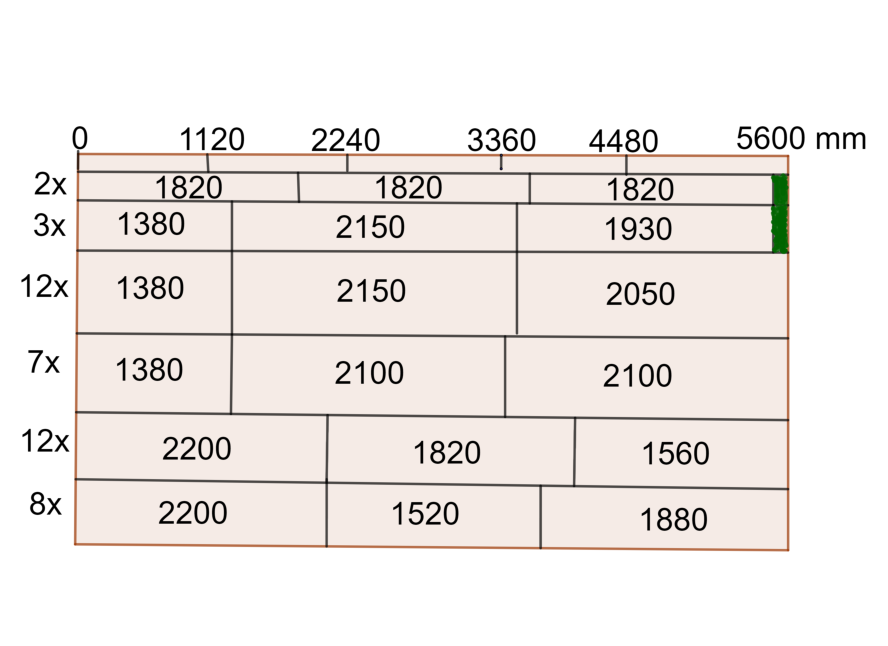
\includegraphics[width=230pt, height=230pt]{cutting_stock.eps}
 	\caption{Rješenje jedne instance.}
 	\label{fig:cuting_stock_solutions}
 \end{figure}
 
 Primjera radi, na  Slici~\ref{fig:cuting_stock_solutions} indeks $1$ odgovara obrascu (dužine) $1820$, indeks $2$ obrascu (dužine) $1380$, indeks 3 obrascu $2150$, indeks 4 obrascu $1930$,   itd.  Nadalje, prvo sječenje sa slike odgovara 
 sljedećim vrijednostima: $a_{1,1}=3, a_{1,2}=a_{1,3}=\ldots =0$, i $x_1 = 2$. Ovo znači da u prvom sječenju visine 2, obrazac 1 (tj. dužina $1820$) se pojavljuje tri puta, dok se ostali obrasci ne pojavljuju ovdje. Drugo sječenje (narudžba) odgovara sljedećim vrijednostima: $a_{1,1}= 0, a_{1,2}=1, a_{1,3}=1, a_{1,4}=0=a_{1,5}=\ldots = 0$, dok je  $x_2 = 3$. Ovo znači da se u drugom sječenju visine 3, obrazac $1820$ ne pojavljuje, obrazac $1380$ pojavljuje jednom, kao i obrasci $2150$  i $1930$, dok se ostali obrasci ne pojavljuju.  

 
 Ideja kojom se vodimo pri konstrukciji algoritma je da se obrasci ne formiraju na početku procedure, već da se generišu prema potrebi (po kolonama), koristeći \emph{metodu generisanja kolona}. Kolona $a$ odgovara dopustivom obrascu akko vrijedi 
 $$ \sum_{i=1}^m a_i w_i \leq W,$$
 gdje vektor $a$ sadrži samo nenegativne (cjelobrojne) vrijednosti. 
 
% Primijetimo da je cijena svakog paterna po kolonama jednaka za svaku kolonu. 
Primijetimo da su, na osnovu prethodnog, razmatrajući relaksaciju problema  $CSILP$, vrijednosti koeficijenata doprinosa 
jednaki $\overline{c} = 1 - \sum_{i} a_{j,i} y_i$.  
 Dakle, CG podproblem izgleda ovako
$$ \begin{array}{lll}
     &\max& \sum_{i=1}^m y_i a_i \\
     & \mbox{t.d}& \\
     &  &\sum_{i} w_i a_i \leq W \hspace{2cm} (CGP)\\
     & &a_i \geq 0 \\
     & &a_i \in \mathbb{Z},
 \end{array}$$
  gdje su $y_i$ vrijednosti optimuma duala. 
  
 
 Ovaj problem je poznat pod nazivom \emph{cjelobrojni problem jednodimenzionalnog ruksaka}. Iako je NP-težak, on se u praksi relativno efikasno rješava  uz pomoć dinamičkog programiranja. 
 

 Za ovaj problem je lako naći inicijalno bazno dopustivo rješenje.
 Za $i$-tu baznu kolonu uzimamo $i$-ti jedinični vektor, tj. obrazac dobijen rezanjem jedne rolne dužine $w_i$. Ovakav skup kolona zaista formira inicijalnu dopustivu bazu. Svakako, malo je vjerovatno da će ove kolone biti korištene u optimalnom rješenju, ali to nije ni očekivano od inicijalnog rješenja. 
 Algoritam za rješavanje ovog problema je sljedeći.
 \begin{enumerate}
     \item Konstruišimo inicijalno bazno dopustivo rješenje (jedinični vektori) i kolone ubacimo u skup $S$.
     \item Riješimo relaksaciju restrikovanog problema ($CSILP$) i vratimo dualno optimalno rješenje. 
     \item Riješimo ($CGP$).
     \item Ako je vrijednost optimalnog rješenja negativna, ubaciti novu kolonu $a$ (koja je rješenje podproblema) u skup $S$. Inače, prekidamo proces jer je optimalno rješenje nađeno. 
     \item Riješiti relaksaciju ($CSILP$) na novom skupu kolona $S$.
 \end{enumerate}
 Primijetimo da je dodavanje nove kolone u $S$ odgovara dodavanju novog obrasca u rješenje. 
 
\begin{primjer} Riješimo sada jednu instancu ovog problema pomocu CG okvira. Recimo da imamo $W = 15$, te tri narudžbe za sječenje:
	\end{primjer}
 \begin{enumerate}
 	\item stavka: $b_1=80$ rolni dužine 4;
 	\item stavka: $b_2=50$ rolni dužine 6;
 	\item stavka: $b_3=100$ rolni dužine 7. 
 \end{enumerate}
 Definišimo sa $A_j = \begin{pmatrix}
                          a_4 \\
                          a_6 \\
                          a_7
                   \end{pmatrix}$
                 patern $j$, koji označava koliko   kojih ronli smo ugradili u veliku rolnu na jediničnu širinu. Enumerišimo sve paterne i otpad koji se generiše njime: 
               $$A_1 = 
               \begin{pmatrix}
               	     3 \\
               	     0 \\
               	     0  
               \end{pmatrix},
               A_2=\begin{pmatrix}
                 	0 \\
                	2 \\
                	0  
               \end{pmatrix}, 
           A_3=\begin{pmatrix}
           	0 \\
           	0 \\
           	2  
         \end{pmatrix},
           A_4=  \begin{pmatrix}
           	2 \\
           	0 \\
           	1  
           \end{pmatrix},
       A_5 = \begin{pmatrix}
       	2 \\
       	1 \\
       	0  
       \end{pmatrix},
   A_6 =\begin{pmatrix}
      	0 \\
        1 \\
      	1  
   \end{pmatrix},$$
sa veličinom otpada 
$$ waste_1 = 3, waste_2 = 3, waste_3 = 1, waste_4 = 0, waste_5 = 1, waste_6 = 2,$$
redom. 
ILP model koji odgovara gore ulaznim podacima je sljedeći:
\begin{align*}
	 &\min x_1 + x_2 + x_3 + x_4 + x_5 + x_6 \\
	 &s.t. \\
	 &\begin{pmatrix}
	 	3 \\
	 	0 \\
	 	0  
	 \end{pmatrix} x_1 + \begin{pmatrix}
	 0 \\
	 2 \\
	 0  
 \end{pmatrix} x_2 +\begin{pmatrix}
 0 \\
 0 \\
 2  
\end{pmatrix} x_3 + 
 \begin{pmatrix}
	2 \\
	0 \\
	1  
\end{pmatrix} x_4 + 
 \begin{pmatrix}
	2 \\
	1 \\
	0  
\end{pmatrix} x_5 + 
\begin{pmatrix}
	0 \\
	1 \\
	1  
\end{pmatrix} x_6 = \begin{pmatrix}
      80 \\
      50 \\
      100
\end{pmatrix} \\
& x_i \geq 0, x_i \in \mathbb{Z}, i=1,\ldots,6.
\end{align*}
 Uzmimo prve tri promjenljive $x_1, x_2$ i $x_3$ koji će generisati početni skup kolona $I$.
 Dakle, imamo sljedeći restrikovani MP:
 \begin{align*}
 	 &\min x_1 + x_2 + x_3 \\
 	 & s.t. \\
 	 &\begin{pmatrix}
 	 	3 \\
 	 	0 \\
 	 	0  
 	 \end{pmatrix} x_1 + \begin{pmatrix}
 	 	0 \\
 	 	2 \\
 	 	0  
 	 \end{pmatrix} x_2 +\begin{pmatrix}
 	 	0 \\
 	 	0 \\
 	 	2  
 	 \end{pmatrix} x_3 = \begin{pmatrix}
  	     80 \\
  	     50 \\
  	     100
  \end{pmatrix} \\
  & x_i \geq 0, x_i \in \mathbb{Z}, i=1,2,3.
 \end{align*}  
Da bismo  problem posmatrali sa jednostavnije strane, izbacimo uslove integralnosti (cjelobrojnosti promjenjivih). Tada ovaj problem možemo da riješimo uz pomoć simpleks metoda, gdje je 
$B^{-1} =\begin{pmatrix}
	    \frac{1}{3} & 0 & 0 \\
	    0 & \frac{1}{2} & 0  \\
	    0 &   0 & \frac{1}{2}
\end{pmatrix}$, dok završna (optimalna) simpleks tabela ima oblik 

\begin{center}
 
\begin{tabular}{cccc|c}
	  $x_1$ &     $\frac{1}{3}$  &   0 & 0  & $\frac{80}{3}$ \\
	  $x_2$ &     0              &  $\frac{1}{2}$  & 0 & $25$ \\
	  $x_3$ &     0              &  0    &  $\frac{1}{2}$  & 50 \\ \hline
	  $z$   &  $\frac{1}{3}$     &  $\frac{1}{2}$   &  $\frac{1}{2}$ & $\frac{305}{3}$ 
\end{tabular}
\end{center}
Sljedeći korak je naći kolonu čiji je koeficijent doprinosa negativan i ubaciti je potom u restrikovani MP u cilju poboljšanja trenutnog rješenja. Dakle, treba da riješimo CGSP
\begin{align}
	\min_{i=1,\ldots,n} \overline{c_j} = \min_{i=1,\ldots,n} 1 - y^T N
\end{align}
gdje su $N$ vektori (kolone) koji odgovaraju nebaznim promjenljivim. Ovaj problem je ekvivalentan rješavanju problema
\begin{align}
	\max_{j=1,\ldots,n} y^T A_j,
\end{align}
gdje su $A_j$ paterni, $j=1,\ldots, 6$. 
Ako je rješenje veće od 0, optimalno rješenje nađeno rješavanjem prethodnog RMP je optimalno i za početni problem. Inače, biramo promjenljivu (i odgovarajuću kolonu) sa minimalnim negativnim doprinosom koju potom ubacujemo u RMP. Kako je svaki patern dat u opštem slučaju kao $A_j = \begin{pmatrix}
	a_4 \\
	a_6 \\
	a_7
\end{pmatrix}$, CG podproblem se svodi na sljedeći optimizacioni problem
\begin{align}
	 \max y_1 a_4 + y_2 a_6 + y_3 a_7  
\end{align}
uz zadovoljenje uslova o maksimalnoj širini
\begin{align}
   &	4 a_4 + 6 a_6 + 7 a_7 \leq 15 \\
   &	a_4, a_6, a_7 \geq 0, a_4, a_6, a_7 \in \mathbb{Z}.
\end{align}
Kako smo to i ranije pomenuli, ovaj problem je klasični problem ruksaka koji se u praksi rješava veoma efikasno. Dakle, ako je rješenje problema ruksaka manje ili jednako od 1, trenutno najbolje rješenje je optimalno rješenje. U protivnom, optimalno rješenje $(a_4^*, a_6^*, a_7^*)^T$ se uključuje  u RMP kao nova kolona. Na osnovu prethodne simpleks tabele imamo $y_1 = \frac{1}{3}, y_2 = y_3 = \frac{1}{2}$, pa treba da riješimo sljedeći CG problem
\begin{align*}
      &\max \frac{1}{3} a_4 + \frac{1}{2} a_6 + \frac{1}{2} a_7 \\
      & 4 a_4 + 6 a_6 + 7 a_7 \leq 15 \\
      & 	a_4, a_6, a_7 \geq 0, a_4, a_6, a_7 \in \mathbb{Z}.
\end{align*}
Pomoću algoritma dinamičkog programiranja, riješimo ovaj problem i dobijamo rješenje 
$(a_4^*, a_6^*, a_7^*)^T =  (2, 0, 1)^T=A_4$, optimalne vrijednosti $\frac{7}{6}$. Konvertujemo vektor $\begin{pmatrix}
	2\\
    0 \\
    1
\end{pmatrix}$
na bazu koja je generisana vektorima baze $x_1$, $x_2$ i $x_3$.  Iz toga slijedi da se vektor 
$$ B^{-1}A_4 = \begin{pmatrix}
	  \frac{2}{3} \\
	  0           \\
	  \frac{1}{3}
\end{pmatrix}$$ uključuje u novu simpleks tabelu (uz redukovanu cijenu doprinosa od -(1- $\frac{7}{6}$)= $\frac{1}{6}$):

\begin{center}
	
	\begin{tabular}{ccccc|c}
		$x_1$ &     $\frac{1}{3}$  &   0 & 0  &      $ \frac{2}{3}$           & $\frac{80}{3}$ \\
		$x_2$ &     0              &  $\frac{1}{2}$  & 0     & 0                 &     $25$ \\
		$x_3$ &     0              &  0    &  $\frac{1}{2}$  & $ \frac{1}{3}$    & 50 \\ \hline
		$z$   &  $\frac{1}{3}$     &  $\frac{1}{2}$   &  $\frac{1}{2}$ &   $\frac{1}{6}$   & $\frac{305}{3}$ 
	\end{tabular}
\end{center}
U novoj koloni tražimo pivot element (kao i u simpleks metodi). Lako je vidjeti da je pivot element $\frac{2}{3}$, pa primjenjujući elementarne transformacije po vrstama oko pivota, dobijamo simpleks tabelu
\begin{center}
	\begin{tabular}{ccccc| c}
		  $x_4$ & $\frac{1}{2}$ & 0 & 0 & 1 & 40 \\
		  $x_2$ & 0 & $\frac{1}{2}$ & 0 & 0 & 25 \\
		  $x_3$ & -$\frac{1}{4}$ & 0 & $\frac{1}{2}$ & 0 & 30 \\ \hline
		  $z$ & $\frac{1}{4}$ & $\frac{1}{2}$ & $\frac{1}{2}$ & 0 & 95 
	\end{tabular}
\end{center}

Dalje, generišimo novi CG podproblem čitajući vrijednost dualnih promjenjivih iz prethodne simpleks tabele $y_1 = \frac{1}{4}$, $y_2 = \frac{1}{2}$, $y_3= \frac{1}{2}$, a dobijamo novi podproblem
\begin{align*}
	 \frac{1}{4} a_4 + \frac{1}{2} a_6 + \frac{1}{2} a_7
\end{align*}
uz uslove nenegativnosti i kapaciteta i integralnosti (cjelobrojnosti). Rješavajući problem dinamičkim programiranjem, dobijamo optimalno rješenje $A_5 = (2,1,0)^T$. Vrijednost optimuma za CG podproblem je jednaka 1, odakle slijedi da je optimum početnog problema pronađen sa prethodnim rješenjem (ne postoji ulazna kolona koje se dodaju u RMP). Rješenje je jednako 95 i dato je sa $x_1^* = 0, x_2^* = 25, x_3^*=30, x_4^*= 40$. Dakle, koristimo samo 3 različita obrasca za sječenje. 
\\ \vspace{1cm}
 %Za uraditi:  https://ocw.mit.edu/courses/sloan-school-of-management/15-083j-integer-programming-and-combinatorial-optimization-fall-2009/lecture-notes/ (Lekcija 19-25)
 \section{Zadaci}
 \begin{enumerate}
 	\item %http://web.tecnico.ulisboa.pt/mcasquilho/compute/_linpro/TaylorB_module_c.pdf
 	Pomoću metode grananja i ograničavanja (B\&B) riješiti sljedeći problem ILP-a
 	\begin{align*}
 		&\max 100 x_1 + 150 x_2 \\
 		&\mbox{t.d.} \\
 		& 8000 x_1 + 4000 x_2 \leq 40 000 \\
 		& 15 x_1 + 30 x_2 \leq 200 \\
 		& x_1, x_2 \geq 0 \\
 		& x_1, x_2 \in \mathbb{Z}.
 	\end{align*}
   \item %http://web.tecnico.ulisboa.pt/mcasquilho/compute/_linpro/TaylorB_module_c.pdf
   	Pomoću metode grananja i ograničavanja  (B\&B) riješiti sljedeći problem ILP-a
   \begin{align*}
   	    &\max 5 x_1 + 4 x_2 \\
   	    &\mbox{t.d.} \\
   	    & 3 x_1 + 4 x_2 \leq 10 \\
   	    & x_1, x_2 \geq 0 \\
   	    & x_1, x_2 \in \mathbb{Z}.
   \end{align*}
Nakon primjene B\&B metode, riješiti problem grafički dijeljeći region na podregione i uoprediti dobijena rješenja. 
\item 	Pomoću metode grananja i ograničavanja  (B\&B) riješiti sljedeći problem ILP-a
\begin{align*}
	 &\max 5x_1 + 6 x_2 + 4 x_3 \\
	 &\mbox{t.d.} \\
	 & 5x_1 + 3 x_2 + 6 x_3 \leq 20 \\
	 & x_1 + 3x_2 \leq 12 \\
	 & x_1,x_2, x_3 \geq 0 \\
	 & x_2 \in \mathbb{Z}.
\end{align*}
\item %http://www.ens-lyon.fr/DI/wp-content/uploads/2012/01/LagrangianRelax.pdf
 Pomoću metode implicitne enumeracije riješiti sljedeći ILP
\begin{align*}
  &\max 1000 x_1 + 700 x_2 + 800 x_3 \\
  &\mbox{t.d.} \\
  & 5000 x_1 + 6000 x_2 + 4000 x_3 \leq 10000 \\
  & x_1, x_2, x_3 \in \{0, 1\}.
\end{align*}
\item  Pomoću metode implicitne enumeracije riješiti sljedeći ILP
\begin{align*}
	 &\max 20 x_1 + 30 x_2 + 10 x_3 + 40 x_4 \\
	 &\mbox{t.d.}\\
	 & 2x_1 + 4 x_2 + 3 x_3 + 7 x_4 \leq 10 \\
	 & 10 x_1 + 7 x_2 + 20 x_3 + 15 x_4 \leq 40 \\
	 & x_1 + 10 x_2 + x_3 \leq 10 \\
	 & x_1, x_2, x_3, x_4 \in \{0, 1\}.
\end{align*}
	\item Metodom Gomorijevih odsjecajućih ravni, riješiti sljedeći ILP% https://homepages.rpi.edu/~mitchj/handouts/gomorycuts/gomorycuts.html
	\begin{align*}
		 &\min -x_1 - x_2 \\
		 &\mbox{t.d.}\\
		 & 2.1 x_1 + 5.2x_2 \leq 20 \\
		 & 4.5 x_1 + 3.5 x_2 \leq 17 \\
		 & x_1, x_2 \geq 0 \\
		 & x_1, x_2 \in \mathbb{Z}.
	\end{align*}
\item Metodom Gomorijevih odsjecajućih ravni, riješiti sljedeći ILP% https://homepages.rpi.edu/~mitchj/handouts/gomorycuts/gomorycuts.html
\begin{align*}
	& \max x_1 + 4 x_2 \\
	& \mbox{t.d.} \\
	& 2 x_1 + 4 x_2 \leq 7 \\
	& 5 x_1 + 3 x_2 \leq 15 \\
	& x_1, x_2 \geq 0 \\
	& x_1, x_2 \in \mathbb{Z}.
	\end{align*}
\item    %http://sisdin.unipv.it/labsisdin/teaching/courses/ails/files/Cutting%20Plane%20Method.pdf
  Uz pomoć algoritma B\&C riješiti sljedeći problem ILP-a
  \begin{align*}
  	 &\max x_1 + 2 x_2 \\
  	 &\mbox{t.d.} \\
  	 & -2x_1 + 2 x_2 \leq 5 \\
  	 & 6 x_1 + 4 x_2 \leq 25 \\
  	 & x_1, x_2 \geq 0 \\
  	 & x_1, x_2\in \mathbb{Z}.
  \end{align*}
\item  Za sljedeći problem 
\begin{align*}
	&\min c^T x \\
	&\mbox{t.d.}\\
	& Ax = b \\
	& D x \geq q \\
	& x \geq 0
\end{align*}
napisati odgovarajuću Lagranžovu relaksaciju. 
\item %https://personal.eur.nl/birbil/bolbilim/teaa/02_Lag_Rel.pdf
Neka je dat problem ILP-a
\begin{align*}
	&\max x_2 \\
    &\mbox{t.d.}\\
	& -2x_1 + 2x_2 \leq 1 \\
	& 2 x_1 + 2 x_2 \leq 7 \\
	& x_1, x_2 \geq 0 \\
	& x_1, x_2 \in \mathbb{Z}.
\end{align*}
Definisati Lagranžovu relaksaciju za ovaj problem (npr. uzeti prvo ograničenje za ,,teško''). Riješiti početni problem sa jednom od tehnika za rješavanje ILP-a. Potom, riješiti Lagranžovu relaksaciju problema za $\lambda=0.25$. Šta možemo zaključiti na osnovu rješenja Lagranžove relaksacije i početnog problema? 
\item   Pomoću CG okvira (generisanje kolona), riješiti jedni instancu \emph{Cutting stock} problema gdje je  
$W = 20$, te postoje tri narudžbe za sječenje: 1. stavka: $b_1=60$ rolni dužine 7; 2. stavka: $b_2=40$ rolni dužine 8; 3. stavka: $b_3=70$ rolni dužine 10. 

 \end{enumerate}
 
 %\newpage
 
 \chapter{Dekompozicione metode}
 
Dekompozicione metode u matematičkom programiranju su tehnike pomoću kojih se polazni problem  razbija u više manjih problema, te se, rješavanjem tih manjih problema, na kraju dolazi i do rješenja polaznog.

Široka primjena metoda linearnog, cjelobrojnog i mješovitog cjelobrojnog linearnog programiranja (MILP) u modelovanju i rješavanju velikog broja različitih problema iz teorije i prakse, doveli su do porasta interesa  za razvoj i primjenu  dekompozicionih metoda. Čak se i tradicionalne metode za rješavanje problema cjelobrojnog programiranja, kao što su B\&B  ili odsjecajuće ravni, takođe   mogu smatrati dekompozicionim metodama, jer one dijele polazni problem na LP relaksaciju i cjelobrojna ograničenja.

Treba napomenuti da i savremeni MILP rješavači, o čemu će biti govora kasnije, takođe, u svojim implementacijama koriste i dekompozicione algoritme, koji, u nekim slučajevima, lakše i brže dovode do rješenja. U ovom poglavlju razmatraćemo dvije standardne dekompozicione metode: Benderovu i Dantzig-Wolfe dekompoziciju.
 
 \section{Benderova dekompozicija}
 
 Benderova metoda je uvedena šezdesetih godina dvadesetog vijeka, kao algoritam za rješavanje MILP programa. 
 Osnovna ideja Benderove dekompozicije primijenjenog na MILP program je podjela skupa promjenljivih na dva podskupa, od kojih se jedan skup promjenljivih (skup cjelobrojnih promjenljivih) smatra ,,komplikovanim'', odnosno skupom promjenljivih čijim se fiksiranjem dolazi do značajnog pojednostavljenja polaznog problema. Prvi problem, koji se naziva i master problem,  rješava se nad prvim skupom promjenljivih, dok se vrijednosti promjenljivih iz drugog skupa,  za dato rješenje prvog podproblema, određuju rješavanjem drugog podproblema. Uspješnu primjenu Benderove dekompozicije, između ostalog, obezbjeđuje i teorija dualnosti, odnosno teoreme o slaboj i jakoj dualnosti.
 

 Posmatrajmo sada sljedeću formulaciju MILP programa
\begin{equation}
 \begin{aligned}\label{bender1}
  &\min\  f^Tx+g^Ty\\
 & \mbox{t.d.}\\
  &Ax+By\geqslant c\\
 &x\geqslant 0,\ y \in \mathbb{Z}
 \end{aligned}
\end{equation}
 gdje su $x$ i $y$ vektori neprekidnih i cjelobrojnih promjenljivih, respektivno, dimenzija $p$ i $q$. $f,g,c$ su vektori, a $A$ i $B$ matrice odgovarajućih dimenzija. 
 
 Pretpostavimo da raspolažemo jednom početnom vrijednošću vektora $y$. Za tu vrijednost (označimo je sa $\overline{y}$) dobijamo sljedeći podproblem

\begin{equation}
	\begin{aligned}\label{bender2}
 			&\min\  f^Tx+g^T\overline{y}\\
 		& \mbox{t.d.}\\
 		& Ax\geqslant c-B\overline{y}\\
 		& x\geqslant 0
 \end{aligned}
\end{equation}

 
Posmatrajmo dualni problem podproblema~(\ref{bender2}), ignorišući sabirak $g^T\overline{y}$, koji je konstantan.

\begin{equation}
	\begin{aligned}\label{bender3}
	&\max\ u^T (c-B\overline{y})\\
 		& \mbox{t.d.}\\
	&u^TA\leqslant f\\
	&u\geqslant 0
 \end{aligned}
\end{equation}


Sada uključujemo teoriju dualnosti i razmatramo sljedeće mogućnosti, koje mogu da se jave.
 
1. Ako je optimalno rješenje problema~(\ref{bender2}) $z^*$, a optimalno rješenje duala~(\ref{bender3}) $u^*$, na osnovu teoreme o jakoj  dualnosti imamo
  \begin{equation}
	\begin{aligned}\label{bender4}
z^*-g^T\overline{y}=(u^*)^T(c-B\overline{y})
	\end{aligned}
\end{equation}


Dalje, uočimo da oblast dopustivih rješenja dualnog problema~(\ref{bender3}) ne zavisi od vrijednosti $\overline{y}$. Stoga, $u^*$ je uvijek dopustivo rješenje problema~(\ref{bender3}), bez obzira na vrijednost $\overline{y}$. Odavde, na osnovu teoreme o slaboj  dualnosti dobijamo

  \begin{equation}
\label{bender5}
		z\geqslant g^Ty+(u^*)^T(c-By)
\end{equation}


Posljednja nejednakost određuje jednju donju granicu funkcije cilja polaznog problema. Ovo je ključni element koji se koristi u Benderovoj dekompoziciji, pomoću kog se određuje jedna odsjecajuća ravan za master problem, koji će biti definisan kasnije. Treba napomenuti da odsjecajuća ravan~(\ref{bender5}) ukazuje na činjenicu da, ako bi se za $y$ uzela vrijednost $\overline{y}$, funkcija cilja bi bila veća ili jednaka vrijednosti $\overline{z}$, koja se dobije u podproblemu, s obzirom da važi $	z\geqslant g^Ty+(u)^T(c-B\overline{y})$.

Ovo takođe daje i donju granicu za druge vrijednosti $y$ koje bismo mogli probati u narednim iteracijama.

2. Posmatrajmo sada slučaj kada je dualni podproblem neograničen. U toj situaciji važi nejednakost
\begin{equation}
	\label{bender6}
	(u^*)^T(c-By)>0
\end{equation}
gdje je ${(u^*)}^T$ vektor koji definiše pravac mogućih rješenja duž kog funkcija neograničeno raste. Ovakav pravac se naziva i \emph{ekstremni zrak}.
 
U ovom slučaju, cilj je eliminisati ovaj zrak iz daljeg razmatranja (budućih rješenja). Da bismo to uradili, potrebno je osigurati da izraz $(u^*)^T(c-By)$ bude manji ili jednak od nule u svim narednim koracima. Tako, master problemu dodajemo novu odsjecajuću ravan, definisanu sa
\begin{equation}
	\label{bender7}
	(u^*)^T(c-By)\leqslant 0
\end{equation}
 
Sada možemo definisati master problem koji nastaje dodavanjem svih odsjecajućih ravni generisanih u prethodnim koracima.
  \begin{equation}
	\begin{aligned}\label{bender8}
		&\min\ z\\
		&\mbox{t.d.} \\
		&z \geq g^Ty+(u^k)^T(c-By) , \ k \in K\\
		& (u^k)^T(c-By) \leq, \ k \in L\\
		&y \in \mathbb{Z},
	\end{aligned}
\end{equation}
 gdje je $K$ skup ekstremnih tačaka, a $L$ skup ekstremnih zrakova podproblema. Rješavanjem master problema (koji je obično puno lakši od početnog problema) dobijamo novu vrijednost za $y$, koju koristimo u sljedećoj iteraciji.
 
 Treba napomenuti da je podproblem~(\ref{bender2}) restrikcija originalnog problema~(\ref{bender1}), pa je njegova optimalna vrijednost $z^*$ jedna gornja granica za funkciju cilja polaznog problema. Takođe, master problem~(\ref{bender8}) je relaksacija polaznog problema, jer se pri rješavanju master problema ne posmatraju sva ograničenja. Stoga, optimalna vrijednost master problema je donja granica za funkciju cilja originalnog problema.
% DOPUNITI
 
 Postupak primjene Benderove dekompozicije na problem minimizacije prikazan je Algoritmom~\ref{alg:bender}.

 
 
 \begin{algorithm}[H] \label{alg:bender}
 	\begin{algorithmic}[1] 
 		\STATE Postavi $\overline{y}\in\mathbb{Z}$ na inicijalnu vrijednost
 		\STATE 	$LB \gets$ $-\infty$; $UB \gets$ $+\infty$
 		\WHILE{$UB-LB>\epsilon$}
 		\STATE Riješi dualni problem (Benderov podproblem)
 		
 		$$	\begin{aligned}
 			\max\ &u^T (c-B\overline{y})\\
 			\mbox{t.d.}\ &u^TA\leqslant f\\
 			&u\geqslant 0.
 			\end{aligned}$$
 		
 		\IF{podproblem nema dopustivo rješenje}
 		\STATE  KRAJ // nema  rješenja  
 		\ENDIF
 		\IF{podproblem ima optimalno rješenje}
 		\STATE $UB \gets \min\{UB,g^Ty+(u^k)^T(c-By)\}$
 		\STATE Generiši Benderovu odsjecajuću ravan $z\geqslant g^Ty+(u^k)^T(c-By)$ i dodaj je u master problem.
 		\ENDIF
		 \IF{podproblem nije ograničen}
		\STATE Generiši Benderovu dopustivu ravan 	$(u^k)^T(c-By)\leqslant 0$ i dodaj je u master problem.
		\ENDIF
		\STATE Riješi Benderov master problem:
			$$\begin{aligned}
			&\min\ z\\
			& {\mbox{t.d.}}\\
			& g^Ty+(u^k)^T(c-By), \ k \in K\\
			& (u^k)^T(c-By), \ k \in L\\
			&y \in \mathbb{Z}
		\end{aligned}$$
			i odredi novu vrijednost $\overline{y}$ i vrijednost rješenja $z^*$.
		\STATE $LB \gets$ $\max\{LB,z^*\}$
 		\ENDWHILE
 	\end{algorithmic}
 	\caption{Benderova dekompozicija}\label{alg:bender}
 \end{algorithm}



U primjeru kojim ilustrujemo upotrebu Benderove dekompozicije posmatramo jedan jednostavan problem maksimizacije dobiti na osnovu ulaganja po različitim kriterijumima.
Iako je Algoritmom~\ref{alg:bender} opisan postupak rješavanja problema minimizacije, algoritam se vrlo lako može preformulisati tako da se može primijeniti i na problem maksimizacije. Jasno je da će u tom slučaju, dualni problem, prikazan u liniji 4 algoritma tada postati problem minimizacije, te će se, rješavanjem dualnog podproblema dobijati donje granice.


\begin{primjer} Pretpostavimo da raspolažemo sumom od 1000KM, koju možemo iskoristiti za ostvarivanje dobiti prema dva različita kriterijuma:
	\end{primjer}
\begin{itemize}
	\item Oročenje novca sa fiksnom kamatom u iznosi od 4.5\%. Dodatno ograničenje je da se može oročiti samo cjelobrojan iznos novca.
	
	\item Ulaganje u neke od 10 vrsta dionica ($f_1, f_2, f_3,\ldots,f_{10}$), sa stopama rasta $1\%,2\%,\ldots,10\%$, respektivno. Za svaku vrstu dionica, može se investirati maksimalno 100KM.
\end{itemize}
Postavlja se pitanje kako treba uložiti početnu količinu novca, tako da se ostvari maksimalna dobit.

\emph{Napomena}. Prije nego što krenemo sa rješavanjem problema, naglasimo da ovako formulisan problem predstavlja pojednostavljenu, i ne previše realističnu verziju problema portfelja u ekonomiji, koji pripada oblasti optimizacije protfelja (eng. protfolio optimization). Inače, realni problem ulaganja novca pripada dvo-kriterijumskoj optimizaciji, gdje se pored maksimizacije profita, minimizuje i rizik ulaganja.  

\emph{Rješenje}. S obzirom na postavku zadatka, jasno je da bi optimalno rješenje trebalo da podrazumijeva da se uloži u dionice $f_5,\ldots,f_{10}$ sa maksimalnim mogućim ulaganjem (po 100KM), dok se ostatak novca oročava sa kamatom od  4.5\%.

Sada ćemo problem formalno definisati i riješiti ga metodom Benderove dekompozicije.

Neka su promjenljive definisane sa:

$x_1,x_2,\ldots,x_{10}$ -- iznos uložen u dionice $f_1, f_2, f_3,\ldots,f_{10}$, respektivno

$y$ -- iznos koji je oročen sa fiksnom kamatom u iznosi od 4.5\%. Sada se problem može formlisati na sljedeći način
\begin{equation}\label{primer:formulacija1}
	\begin{aligned}
		&\max\ 1.01x_1+1.02x_2+\ldots+1.10x_{10}+1.045y\\
		&\mbox{t.d.}\\ 
		&x_1+x_2+\ldots+x_{10}+y\leqslant1000\\
		&x_1\leqslant 100\\
		&\vdots \\
		&x_{10}\leqslant 100\\
		&y\in \mathbb{Z}\\
		&x_1,x_2,\ldots,x_{10},y\geqslant 0
	\end{aligned}
\end{equation}

Zapišimo sada model u obliku koji odgovara postavci metoda Benderove dekompozicije.
 \begin{equation}\label{primer:formulacija2}
	\begin{aligned}
		&\max\  f^Tx+g^Ty\\
			&\mbox{t.d.}\\ 
		  &Ax+By\leqslant c\\
		&x\geqslant 0,\ y \in \mathbb{Z}^+
	\end{aligned}
\end{equation}
gdje je


$$x=\left(\begin{array}{c}
	x_1 \\
	x_2 \\
	\vdots \\
	x_{10}
\end{array}\right) ,  
 f = \left(\begin{array}{c}
	1.01 \\
	1.02 \\
	\vdots \\
	1.10
\end{array}\right)$$

Primijetimo da su u našem primjeru $g$ i $y$ jednodimenzioni vektori, koje ćemo u daljem zapisu identifikovati sa njihovom (jedinom) koordinatom, odnosno
$y=(y)$ i $g=(1.045)$. Takođe je i 

$A=\left(
\begin{array}{ccc}
	1 & \ldots & 1 \\
	1 & \ldots & 0 \\
	\vdots & \ddots & \vdots \\
	0 & \ldots & 1
\end{array}\right)$, \quad
$B=\left(\begin{array}{c}
	1 \\
	0 \\
	\vdots \\
	0
\end{array}\right)$ i \quad 
$c=\left(\begin{array}{c}
	1000 \\
	100 \\
	\vdots \\
	100
\end{array}\right)$ 


Primijenimo sada Benderovu dokompoziciju. Najprije treba odrediti početnu vrijednost za $\overline{y}$, za koju, u ovom koraku, možemo uzeti bilo koju nenegativnu vrijednost. Neka je, na primjer, $\overline{y}=1500$. Dalje, neka su $LB=-\infty$ i $UB=+\infty$ i uzmimo da je $\epsilon = 0.1$.

 Nakon inicijalnih postavki, prvi korak je rješavanje dualnog problema (Benderovog podproblema). S obzirom da je početni problem problem maksimizacije, dualni problem će sada biti problem minimizacije. Obilježimo promjenljive dualnog problema vektorom  $u$, koji ima 11 koordinata (polazni problem ima 11 oraničenja).
 
 Računamo funkciju cilja dualnog problema
 $$
u^T (c-B\overline{y})=(u_1\ldots u_{11})\cdot \left(\left(\begin{array}{c}
	1000 \\
	100 \\
	\vdots \\
	100
\end{array}\right)-\left(\begin{array}{c}
1500 \\
0 \\
\vdots \\
0
\end{array}\right)\right) = -500u_1+100u_2+\ldots+100u_{11}
$$
dok su ograničenja dualnog problema

$$
\begin{aligned}
	u_1+u_2&\geqslant 1.01\\
	u_1+u_3&\geqslant 1.02\\
	\vdots&\\
	u_1+u_{11}&\geqslant 1.1\\
	u_1&\geqslant 1.045\\ 
	u&\geqslant 0\\
\end{aligned}
$$

Lako se vidi da rješenje dualnog problema nije ograničeno (sa donje strane), za $u_1 = +\infty$, $u_2 = u_3=\ldots u_{11}=0$.
Odnosno, 
$$u=\left(\begin{array}{c}
 1 \\
	0 \\
	\vdots \\
	0
\end{array}\right)$$ je ekstremni zrak.

Prateći tok algoritma, određujemo odsjecajuću ravan

$$u^{T}(c-By)\geqslant 0$$
odnosno
$$1000-y\geqslant 0$$
Sada rješavamo master problem


\begin{align*}
	&\max z\\
	&\mbox{t.d.} \\
	&1000-y\geqslant 0\\
	&y\in\mathbb{Z}^+\\	
\end{align*}
Vidimo da, bez obzira na vrijednost $y$, vrijednost funkcije cilja nije ograničena.
Drugim riječima, ako uzmemo bilo koju dopustivu vrijednost za $y$ (recimo $\overline{y}=1000$) dobijamo da je $\overline{z} = +\infty$. Sada možemo zaključiti da u prvoj iteraciji algoritma nismo uspjeli da smanjimo gornju granicu, te nam ostaje $UB = +\infty$.

 Prelazimo na sljedeću iteraciju. Formulišimo novi dualni problem.
 
  Računamo novu funkciju cilja dualnog problema sa vrijednošću $\overline{y}=1000$
 $$
 u^T (c-B\overline{y})=(u_1\ldots u_{11})\cdot \left(\left(\begin{array}{c}
 	1000 \\
 	100 \\
 	\vdots \\
 	100
 \end{array}\right)-\left(\begin{array}{c}
 	1000 \\
 	0 \\
 	\vdots \\
 	0
 \end{array}\right)\right) = 100u_2+\ldots+100u_{11}
 $$
 Imajući u vidu ograničenja dualnog problema, zaključujemo da za vrijednost vektora $$u=\left(\begin{array}{c}
 	1.1 \\
 	0 \\
 	\vdots \\
 	0
 \end{array}\right)$$
funkcija cilja ima minimalnu vrijednost jednaku 0.

Sada ćemo moći da popravimo donju granicu, odnosno

$$LB = \max\{LB,g^Ty+(u)^T(c-By)\}=\max\{-\infty,1.045*1000+0\} = 1.045.$$

Dalje, dodajemo odsjecajuću ravan kao ograničenje master problema:
$$z\leqslant g^Ty+(u)^T(c-By),$$ 
odnosno
$$z\leqslant 1.045y+\left(\begin{array}{c}
	1.1 \\
	0 \\
	\vdots \\
	0
\end{array}\right)^T
\left(\left(\begin{array}{c}
	1000 \\
	100 \\
	\vdots \\
	100
\end{array}\right)-\left(\begin{array}{c}
1 \\
0 \\
\vdots \\
0
\end{array}\right)y\right)$$
$$z\leqslant 1.045y+\left(\begin{array}{c}
	1.1 \\
	0 \\
	\vdots \\
	0
\end{array}\right)^T
\left(\begin{array}{c}
	1000-y \\
	100 \\
	\vdots \\
	100
\end{array}\right)$$
Odnosno

$$z\leqslant 1100-0.055y$$

Sada novodobijenu odsjecajuću ravan dodajemo ograničenjima master problema i rješavamo master problem

$$
\begin{aligned}
	\max z\\
	1000-y\geqslant 0\\
	z\leqslant 1100-0.055y\\ 
	y\in\mathbb{Z}^+\\	
\end{aligned}
$$

Nije teško odrediti da je optimalna vrijednost funkcije cilja master problema $\overline{z}=1100$, koja se dobija za vrijednost $\overline{y}=0$.
Sada možemo da ažuriramo gornju granicu koristeći vrijednost funkcije cilja, odnosno

$$UB = \min\{UB,\overline{z}\} = 1100$$

Pošto je razlika između gornje i donje granice još uvijek veća od $\epsilon$ ($UB-LB = 1100-1045=55$), prelazimo na sljedeću iteraciju.

Uzimamo $\overline{y}=0$ i ponovo rješavamo dualni problem.

Funkcija cilja dualnog problema sada izgleda 

 $$
u^T (c-B\overline{y})=(u_1\ldots u_{11})\cdot \left(\left(\begin{array}{c}
	1000 \\
	100 \\
	\vdots \\
	100
\end{array}\right)-\left(\begin{array}{c}
	0 \\
	0 \\
	\vdots \\
	0
\end{array}\right)\right) =1000u_1+ 100u_2+\ldots+100u_{11}.
$$

S obzirom na ograničenja u dualnom problemu, funkcija ima minimalnu vrijednost 1055 za vektor $$u=\left(\begin{array}{c}
	0\\
	1.01 \\
	1.02 \\
	\vdots \\
	1.1
\end{array}\right).$$

Pošto dual ima optimalno rješenje, računamo novu donju granicu, odnosno,


$$LB = \max\{LB,g^Ty+(u)^T(c-By)\}=\max\{1.045,0+ 1055\} = 1055$$.

Dobijamo novu odsjecajuću ravan koju ćemo pridodati za rješavanje master problema

$$z\leqslant 1.045y+\left(\begin{array}{c}
	0\\
	1.01 \\
	\vdots \\
	1.1
\end{array}\right)^T
\left(\left(\begin{array}{c}
	1000 \\
	100 \\
	\vdots \\
	100
\end{array}\right)-\left(\begin{array}{c}
	1 \\
	0 \\
	\vdots \\
	0
\end{array}\right)y\right).$$
Odnosno 
$$z\leqslant 1.045y+1055$$

Sada novi master problem izgleda 


$$
\begin{aligned}
	\max z\\
	1000-y\geqslant 0\\
	z\leqslant 1100-0.055y\\ 
	z\leqslant 1.045y+1055\\
	y\in\mathbb{Z}^+\\	
\end{aligned}
$$


Rješavanjem ovog problema cjelobrojnog programiranja (na primjer, pomoću nekog od računarskih programa) dobija se optimalno rješenje za cjelobrojnu vrijednost $\overline{y}=41$, koje iznosi $\overline{z} = 1097.745$

Sada možemo da ažuriramo i gornju granicu, odnosno 

$$UB = \min\{1100,\overline{z}\} =  \min\{1100,1097.745\} =1097.745$$

Računamo razliku između gornje i donje granice

$$UB-LB=1097.745-1055 = 42.745$$
i pošto je razlika još uvijek veća od $\epsilon$, nastavljamo dalje sa iterativnim postupkom.

Uzmimo $\overline{y}=41$ i ponovo formirajmo i riješimo dualni problem. 
Funkcija cilja dualnog problema sada izgleda 
$$\min 959u_1+ 100u_2+\ldots+100u_{11},$$

a rješavanjem problema uz data ograničenja dobijamo optimalno rješenje 1013.59, za vrijednosti vektora 
$$u=\left(\begin{array}{c}
	1.01 \\
	0 \\
	0.01\\
	0.02\\
	\vdots \\
	0.09
\end{array}\right)$$

Ažuriranjem donje granice dobija se 
$$LB = \max\{1055,1.045\cdot41+1013.59\} = \max\{1055,1056.435\} = 1056.435 $$

Dalje, dodajemo novu odsjecajuću ravan

$$z\leqslant 1.045y+\left(\begin{array}{c}
	1.01 \\
	0 \\
	0.01\\
	0.02
	\vdots \\
	0.09
\end{array}\right)^T
\left(\left(\begin{array}{c}
	1000 \\
	100 \\
	\vdots \\
	100
\end{array}\right)-\left(\begin{array}{c}
	1 \\
	0 \\
	\vdots \\
	0
\end{array}\right)y\right).$$
Odnosno 
$$z\leqslant 1.045y+1010-1.01y+100\cdot0.45$$
t.j.
$$z\leqslant 0.035y+1055$$

Ovo ograničenje dodajemo master problemu, koji sada izgleda


$$
\begin{aligned}
	\max z\\
	1000-y\geqslant 0\\
	z\leqslant 1100-0.055y\\ 
	z\leqslant 1.045y+1055\\
	z\leqslant 0.035y+1055\\
	y\in\mathbb{Z}^+\\	
\end{aligned}
$$

Rješavanjem ovog master problema dobijamo optimalno rješenje 
 za cjelobrojnu vrijednost $\overline{y}=500$, koje iznosi $\overline{z} = 1072.5$.
 
 Ažuriramo i gornju granicu

$$UB = \min\{1097.745, 1072.5\} =  1072.5.$$

Računamo razliku između gornje i donje granice $1072.5-1056.435$, što je još uvijek veće od $\epsilon$, pa prelazimo na narednu iteraciju.

Uzimamo 
$\overline{y}=500$ i formiramo novi dualni problem sa funkcijom cilja

$$\min 500u_1+ 100u_2+\ldots+100u_{11},$$

čija optimalna vrijednost iznosi 540, za vrijednost vektora $u$

$$u=\left(\begin{array}{c}
	1.05\\
	0\\
	0\\
	0\\
	0\\
	0\\
	0.01 \\
	0.02 \\
	\vdots \\
	0.05
\end{array}\right).$$

Ažuriramo donju granicu,
$$LB = \max\{1056.435, 1.045\cdot 500+540\} =1062.5 $$


Dalje, master problemu pridružujemo odsjecajuću ravan
 
 
 $$z\leqslant 1.045y+\left(\begin{array}{c}
 	1.05\\
 0\\
 0\\
 0\\
 0\\
 0\\
 0.01 \\
 0.02 \\
 \vdots \\
 0.05
 \end{array}\right)^T
 \left(\left(\begin{array}{c}
 	1000 \\
 	100 \\
 	\vdots \\
 	100
 \end{array}\right)-\left(\begin{array}{c}
 	1 \\
 	0 \\
 	\vdots \\
 	0
 \end{array}\right)y\right).$$
 Odnosno 
 $$z\leqslant 1.045y+1050-1.05y+100\cdot0.15$$
 t.j.
 $$z\leqslant -0.005y+1065$$
 
 
 Kada i ovo ograničenje dodamo master problemu, dobijamo novi master problem
 
 $$
 \begin{aligned}
 	&\max z\\
 	&\mbox{t.d.}\\
 	&1000-y\geqslant 0\\
 	&z\leqslant 1100-0.055y\\ 
 	&z\leqslant 1.045y+1055\\
 	&z\leqslant 0.035y+1055\\
 	&z\leqslant -0.005y+1065\\
 	&y\in\mathbb{Z}^+\\	
 \end{aligned}
 $$
 

 
 čije se optimalno rješenje iznosi $\overline{z} = 1063.75$, a dobija se za cjelobrojnu vrijednost $\overline{y}=250$.
 
 Ažuriranjem gornje granice dobijamo 
 $$UB = 1063.75,$$ 
 pa je razlika između gornje i donje granice jednaka
 $1063.75-1062.5=1.25$, što je još uvijek veće od $\epsilon$.
 
Ponovo formiramo dualni problem uzimajući $\overline{y}=250$.
 
 Nova funkcija cilja sada izgleda
 $$\min 750u_1+ 100u_2+\ldots+100u_{11},$$
 
 a optimalna vrijednost funkcije cilja je 800.5 za vrijednost vektora $u$
 
 
 $$u=\left(\begin{array}{c}
 	1.03\\
 		0\\
 		0\\
 		0\\
 0.01\\
 0.02\\
 0.03\\
 0.04\\
 0.05\\
 	1.06\\
 	1.07 \\
 \end{array}\right).$$
 
 Ispitujemo da li se ažurira donja granica:
 $$LB = \max\{1062.5, 1.045\cdot 250+ 800.5\} = \max\{1062.5,1061.75\}=1062.5.$$
 
 Dalje, određujemo odsjecajuću ravan
 
 
 $$z\leqslant 1.045y+\left(\begin{array}{c}
 	1.03 \\
 	0 \\
 	0\\
 	0\\
 	0.01\\
 	0.02\\
 	0.03\\
 	0.04\\
 	0.05\\
 	0.06\\
 	0.07
 \end{array}\right)^T
 \left(\left(\begin{array}{c}
 	1000 \\
 	100 \\
 	\vdots \\
 	100
 \end{array}\right)-\left(\begin{array}{c}
 	1 \\
 	0 \\
 	\vdots \\
 	0
 \end{array}\right)y\right).$$
 Odnosno 
 $$z\leqslant 1.045y+1030-1.03y+28,$$
 t.j.
 $$z\leqslant 0.015y+1058$$
 
 i dodajemo je master problemu, koji izgleda
  $$
 \begin{aligned}
 	&\max z\\
 	&\mbox{t.d.}\\
 	&1000-y\geqslant 0\\
 	&z\leqslant 1100-0.055y\\ 
 	&z\leqslant 1.045y+1055\\
 	&z\leqslant 0.035y+1055\\
 	&z\leqslant -0.005y+1065\\
 	&z\leqslant 0.015y+1058\\
 	&y\in\mathbb{Z}^+\\	
 \end{aligned}
 .$$
 
 Rješavanjem master problema dobijamo novu vrijednost $\overline{y} =350$, a gornja granica se ažurira na 
 $$UB = 1063.25.$$
 
 Ponavljajući postupak još jednom, dobijamo redom: 
 \begin{itemize}
 	\item 
 vrijednost funkcije duala 697,
 \item vektor 
  $$u=\left(\begin{array}{c}
 	1.04\\
 	0\\
 	0\\
 	0\\
 	0\\
 	0.01\\
 	0.02\\
 	0.03\\
 	0.04\\
 	0.05\\
 	1.06\\
 \end{array}\right)$$
\item $LB = 1062.75$,
\item odsjecajuću ravan:  $z\leqslant 0.005y+1061$.
\end{itemize}


Rješavajući još jednom master problem, koji sada izgleda

  $$
\begin{aligned}
	&\max z\\
	&\mbox{s.t.}\\
	&1000-y\geqslant 0\\
	&z\leqslant 1100-0.055y\\ 
	&z\leqslant 1.045y+1055\\
	&z\leqslant 0.035y+1055\\
	&z\leqslant -0.005y+1065\\
	&z\leqslant 0.015y+1058\\
	&z\leqslant 0.005y+1061\\
	&y\in\mathbb{Z}^+\\	
\end{aligned}
$$
dobijamo da je nova vrijednost $\overline{y}=400$, a gornja granica $UB = 1063$.

Formirajući i rješavajući (pokazaće se, po posljednji put), dualni problem, dobija se optimalno rješenje 645, pa donja granica iznosi 1063.

Vidimo da smo dobili da je donja granica jednaka gornjoj i možemo obustaviti iterativni postupak.

Sada znamo da se optimalno rješenje polaznog problema~(\ref{primer:formulacija2}), odnosno~(\ref{primer:formulacija1}), dobija za vrijednost $\overline{y}=400$, te se on svodi na problem

 \begin{equation}\label{primer:formulacija3}
	\begin{aligned}
		\max\  &f^Tx\\
		s.t.\  &Ax\leqslant c-B\overline{y}\\
		&x\geqslant 0
	\end{aligned}
\end{equation}
čije je rješenje predstavljeno vektorom

$$x =\left(\begin{array}{c}
	0\\
	0\\
	0\\
	0\\
	0\\
	100\\
	100\\
	100\\
	100\\
	100\\
	100\\
\end{array}\right)$$



  \section{Dantzig--Wolfe dekompozicija}%https://www.maxwell.vrac.puc-rio.br/29077/29077_5.PDF
 %https://www.youtube.com/watch?v=wxz0NJvKZNM
 %Glavni link: https://www.youtube.com/watch?v=IposxYVBUnY
 
 U ovom odjeljku ćemo objasniti još jednu korisnu dekompozicionu tehniku za rješavanje problema linearnog programiranja -- \emph{Dantzig-Wolfe} (DW) dekompoziciju. Ova tehnika je originalno dizajnirana za rješavanje problema linearnog programiranja velikih dimenzija. Osnovna ideja DW dekompozicije je da se na podskup ograničenja polaznog problema primijeni \emph{Teorema Minkovskog}, odnosno \emph{Teorema o reprezentaciji za konveksne poliedre}, te da se polazni problem razbije na   više manjih podproblema.
 
 \begin{thm}
 	Neka je $P = \{ x \in \mathbb{R}^n \mid Ax \leq b\}$ ograničeni poliedar i neka je $\{x^{(1)}, \ldots, x^{(p)} \}$ skup ekstremnih tačaka poliedra $P$. Tada za sve $x \in P$ vrijedi 
 	 $$ x = \sum_{i=1}^p \lambda_i x^{(i)},$$ 
 	 gdje je $\lambda_i \geq 0,i=1,\ldots,p$, $\sum_{i=1}^p \lambda_i=1$.
 \end{thm}
 
 Pođimo od kanonske formulacije problema linearnog programiranja
 
  \begin{equation}
 	\begin{aligned}\label{dw1}
 		&\min\ c^Tx\\
 		&\mbox{t.d.}\\
 	 &Ax=b\\
 		&x \in X
 	\end{aligned}
 \end{equation}
 
 gdje je skup $X$ poliedar. Iako za DW dekompoziciju nije neophodno, u daljem razmatranju, radi lakše analize DW dekompozicije, smatraćemo da je $X$ ograničen poliedar, odnosno politop.
 
 Dalje, navešćemo i sljedeću pretpostavku. Ako bismo iz skupa ograničenja izbacili ograničenja $Ax=b$, tada bi rješavanje problema bilo jednostavno. Drugim riječima, skup $X$ je opisan nekim ,,jednostavnim'' ograničenjima, dok ograničenja $Ax=b$ čine problem značajno težim, pa ćemo ih, zbog toga, zvati ,,komplikovanim ograničenjima''. 
 
 Posmatrajmo sada konfiguraciju za primjenu Teoreme o reprezentaciji za konveksne poliedre na skup $X$.
 
 Neka su tačke $x^{(1)},x^{(2)},\dots,x^{(t)}$ vrhovi politopa $X$.  
 Prema Teoremi o reprezentaciji za konveksne poliedre, za svaku tačku $x\in X$ vrijedi da se ona može predstaviti kao konveksna kombinacija (ekstremnih) tačaka $x^{(1)},x^{(2)},\dots,x^{(t)}$.
 
 Neka je  $x \in X$ proizvoljna tačka iz skupa $X$.  Tada postoje $\lambda_1,\lambda_2,\ldots,\lambda_t$, takvi da važi:
 \begin{equation}
 	\begin{aligned}
 		&x = \sum_{j=1}^t\lambda_jx^{(j)}\\
 		 &\sum_{j=1}^t\lambda_j = 1\\
 		&\lambda_j\geqslant 0,\ j = 1,\ldots,t
 	\end{aligned}
 \end{equation}
 
 Ponovimo da Teorema o reprezentaciji za konveksne poliedre ima svoju formulaciju i u slučaju da poliedar nije ograničen, ali zbog pojednostavljenja daljeg objašnjenja DW dekompozicije, ovaj slučaj nećemo razmatrati.
 
 Uzimajući u obzir prikazanu reprezentaciju proizvoljne tačke $x\in X$, početni problem~(\ref{dw1}) sada možemo preformulisati na
 
 
   \begin{equation}
 	\begin{aligned}\label{dw2}
 	&	\min\  c^T\cdot \sum_{j=1}^t\lambda_jx^{(j)}\\
 		&\mbox{t.d.}\\  
 		&A\cdot \sum_{j=1}^t\lambda_jx^{(j)}=b\\
 		 		 &\sum_{j=1}^t\lambda_j = 1\\
 		&\lambda_j\geqslant 0,\ j = 1,\ldots,t
 	\end{aligned}
 \end{equation}
odnosno
    \begin{equation}
 	\begin{aligned}\label{dw3}
 		&\min\  \sum_{j=1}^t(c^T x^{(j)})\lambda_j\\
 			&\mbox{t.d.}\\   
 		&\sum_{j=1}^t (A x^{(j)})\lambda_j=b\\
 		&\sum_{j=1}^t\lambda_j = 1\\
 		&\lambda_j\geqslant 0,\ j = 1,\ldots,t
 	\end{aligned}
 \end{equation}
 
 Vidimo da se početni problem~(\ref{dw1}) sada može predstaviti ekvivalentnom reprezentacijom~(\ref{dw3}), u kojoj se, umjesto polaznih promjenljivih (vektora $x$), sada posmatraju promjenljive $\lambda_j,\ j = 1,\ldots,t$, uz pretpostavku da su  vrhovi $x^{(1)},x^{(2)},\dots,x^{(t)}$ konveksnog politopa $X$ poznati.
 
 Skup promjenljivih $\lambda_j,\ j = 1,\ldots,t$ ćemo zvati $\lambda$ promjenljive.
  Variranjem vrijednosti $\lambda$ promjenljivih po dopustivom skupu iz formulacije~(\ref{dw3}), generišu se tačke iz dopustivog skupa polazne formulacije~(\ref{dw1}). Sa druge strane, svaka tačka $x$ iz formulacije~(\ref{dw1}) ima svoju reprezentaciju preko odgovarajućih vrijednosti  $\lambda$ promjenljivih u dopustivom skupu formulacije~(\ref{dw3}). S obzirom na to da i funkcije cilja odgovaraju jedna drugoj, zaključujemo da je i optimalno rješenje polaznog problema~(\ref{dw1}) jednako optimalnom rješenju reformulisanog problema~(\ref{dw3}).
 
 Samom reformulacijom polaznog problema~(\ref{dw1}) u DW formulaciju~(\ref{dw3}) nismo mnogo postigli, jer broj vrhova politopa, a time i broj $\lambda$ promjenljivih može biti jako veliki.
 
 Međutim, pravi razlog za DW dekompoziciju leži u činjenici da za rješavanje problema~(\ref{dw3}) ne moramo eksplicitno da koristimo sve vrhove politopa $X$. Umjesto toga, krenućemo od jednog   manjeg podskupa, a samim tim i podskupom skupa $\lambda$ promjenljivih. Nakon toga, primijenićemo tehniku ,,generisanja kolona'' (eng. \emph{column generation}), kako bismo u razmatranje uključili nove vrhove politopa $X$, koji će pomoći poboljšanju rješenja tzv. ograničenog master problema (eng. \emph{Restricted master problema} -- RMP).
 

 Označimo sada problem formulisan  sa~(\ref{dw3}) kao \emph{Master problem} (MP). Na osnovu master problema formiramo RMP sa manjim brojem $\lambda$ promjenljivih.
 
     \begin{equation}
 	\begin{aligned}\label{dw4}
 		&\min\   \sum_{j\in I}(c^T x^{(j)})\lambda_j\\
 		&\mbox{t.d.}\\ 
 		 &\sum_{j\in I} (A x^{(j)})\lambda_j=b\\
 		&\sum_{j\in I}\lambda_j = 1\\
 		&\lambda_j\geqslant 0,\ j  \in I
 	\end{aligned}
 \end{equation}
gdje je $I$ skup indeksa onih vrhova politopa koji su uključeni u RMP.

Označimo sa $\overline{z}$ optimalnu vrijednost funkcije cilja RMP, a sa $z^*$ optimalnu vrijednost master problema.

Primijetimo da je $\overline{z}$ jedna gornja granica za master problem, jer je svako dopustivo rješenje RMP takođe i dopustivo za master problem. Ova konstatacija će nam biti od koristi u razmatranju koje slijedi.

Da bismo provjerili da li je optimalno rješenje RMP ujedno i optimalno rješenje master problema, potrebno je da provjerimo da li su koeficijenti doprinosa svih nebaznih promjenjivih nenegativni, tj. postoji li neka nebazna promjenljiva koja može doprinijeti dodatnom smanjenju vrijednosti funkcije cilja. Na osnovu karakteristika (optimalne) simpleks tabele i tvrđenja koja važe na osnovu teorije dualnosti, ove vrijednosti su ekvivalentne optimalnim vrijednostima dualnih promjenjivih (duala problema RMP).   
%je reduced cost od svih nebazičnih promjenljivih NIJE JASNO...


%i trebamo optimalne vrijednosti dualnih promjenljivih

Označimo vektorom $y$ optimalne vrijednosti dualnih promjenljih koje se odnose na ograničenja $\sum_{j\in I} (A x^{(j)})\lambda_j=b$ i skalarom $\alpha$ optimalnu vrijednost dualne promjenljive koja se odnosi na ograničenje $\sum_{j\in I}\lambda_j = 1$. 

Da bi se odredili   koeficijenti doprinosa za $\lambda_j$, odredimo šta se dobija u odgovarajućoj koloni. U funkciji cilja, imamo $c^Tx^{(j)}$, u ograničenjima $A x^{(j)} $ i još jednu jedinicu (na osnovu ograničenja $\sum_{j\in I}\lambda_j = 1$). Tako, kolona na koju se fokusiramo da bismo izračunali doprinose izgleda ovako


 $$\left(\begin{array}{c}
 	c^T x^{(j)}\\
 	A x^{(j)} \\
 	1 
 \end{array}\right)$$
 
 Sada rješavamo   podproblem generisanja kolona (skraćeno CG podproblem), čiji je cilj da se pronađe najmanji koeficijent doprinosa. Ukoliko je koeficijent manji od nule, dobija se nova kolona koja treba da se doda u podproblem RMP.  U slučaju da je nenegativan, tada  optimalno rješenje RMP predstavlja ujedno i optimalno rješenje MP.
 
 CG podproblem se definiše kao
 
      \begin{equation}
 	\begin{aligned}\label{dw6}
 		\min_{j=1,\ldots,t}\  & \{c^T x^{(j)} -y^T	Ax^{(j)}-\alpha\cdot 1\}=\min_{x\in X}\  & \{c^Tx-y^T	Ax-\alpha\}\\
 	\end{aligned}
 \end{equation}
 
jer je rješenje problema na desnoj strani jednakosti upravo u nekom od vrhova politopa $X$.

Prisjetimo se sada da smo za jednu od polaznih pretpostavki imali da je skup $X$ opisan kao skup sa ,,jednostavnim'' ograničenjima, što znači da je problem na desnoj strani jednakosti (\ref{dw6}) jednostavan za rješavanje.

Reformulišimo  CG podproblem sada kao problem maksimizacije, gdje ćemo za funkciju cilja uzeti negativnu vrijednost funkcije cilja minimizacije, tj.
 
 
       \begin{equation}
 	\begin{aligned}\label{dw7}
 		\max_{j=1,\ldots,t}\  &  \{y^T	Ax^{(j)}-c^Tx^{(j)}+\alpha\}\\
 	\end{aligned}
 \end{equation}
Neka je $\hat{z}$ optimalna vrijednost funkcije cilja ovog problema maksimizacije.

Posmatrajmo sada jedno dopustivo rješenje $x$ polaznog problema. Za to rješenje važi 
$x\in X$ i $Ax=b$, pa imamo da vrijedi %Za to rješenje $x$ važi 	
 $$y^T	Ax-c^Tx+\alpha\leqslant \hat{z} \Leftrightarrow c^Tx\geqslant y^T	Ax+\alpha-\hat{z} \Leftrightarrow  c^T x \geqslant y^T b+\alpha-\hat{z}.$$
 
 Primijetimo sada da je  $y^T b+\alpha$ zapravo  optimalna vrijednost funkcije duala od RMP, koja je dalje, jednaka optimalnoj vrijednosti $\overline{z}$ od RMP-a. 
 
 $$ c^Tx\geqslant \overline{z}-\hat{z}$$
 
 Sada zaključujemo da je razlika između optimalne vrijednosti RMP-a i problema maksimizacije CG  problema donja granica za originalni LP. Pošto ovo važi za proizvoljno rješenje $x$, zaključujemo da važi 
 $$z^*\geqslant \overline{z}-\hat{z}.$$
 
 Ovim smo dobili da je razlika $\overline{z}-\hat{z}$ donja granica za optimalnu vrijednost funkcije cilja polaznog problema. Dalje, prisjetimo se da je $\overline{z}$ gornja granica za $z^*$, odnosno važi 
\begin{equation}\label{dw8}
	  \overline{z}\geqslant z^*\geqslant \overline{z}-\hat{z}.
\end{equation}
 
 Izraz~(\ref{dw8}) se može koristiti za određivanje koliko  se optimalno rješenje polaznog problema razlikuje od rješenja koja se dobijaju u iterativnom procesu DW dekompozicije.
 
 U slučaju kada je $\hat{z}$ jednako nuli, iz~(\ref{dw8}) se vidi da je vrijednost $\overline{z}$ zapravo i optimalno rješenje polaznog problema.
 
\begin{primjer}%http://eaton.math.rpi.edu/faculty/Mitchell/courses/matp6640/notes/09C_egdcmpbeamer.pdf
 
 Posmatrajmo problem linearnog programiranja
 \end{primjer}
   \begin{equation}
 	\begin{aligned}\label{primjer:dw1}
 		&\max\  x_1\\
 		&\mbox{t.d.}\\  
 		&x_1+3x_2\leqslant \frac94\\
 		 &2x_1-3x_2\leqslant 0\\
 		&x \in X=\{(x_{1,2}):0\leqslant x_{1, 2}  \leqslant 1\}.
 	\end{aligned}
 \end{equation}
 
 Vidimo da u ovom problemu imamo dva ,,komplikovana'' ograničenja ($x_1+3x_2\leqslant \frac94$ i
 $2x_1-3x_2\leqslant 0$). Dalje, vidimo da je skup $X$ definisan kao jedinični kvadrat, što u našem slučaju to znači da je riječ o ,,jednostavnom'' ograničenju. 
 
 \begin{figure}\label{fig:dw1}
 	\centering
 	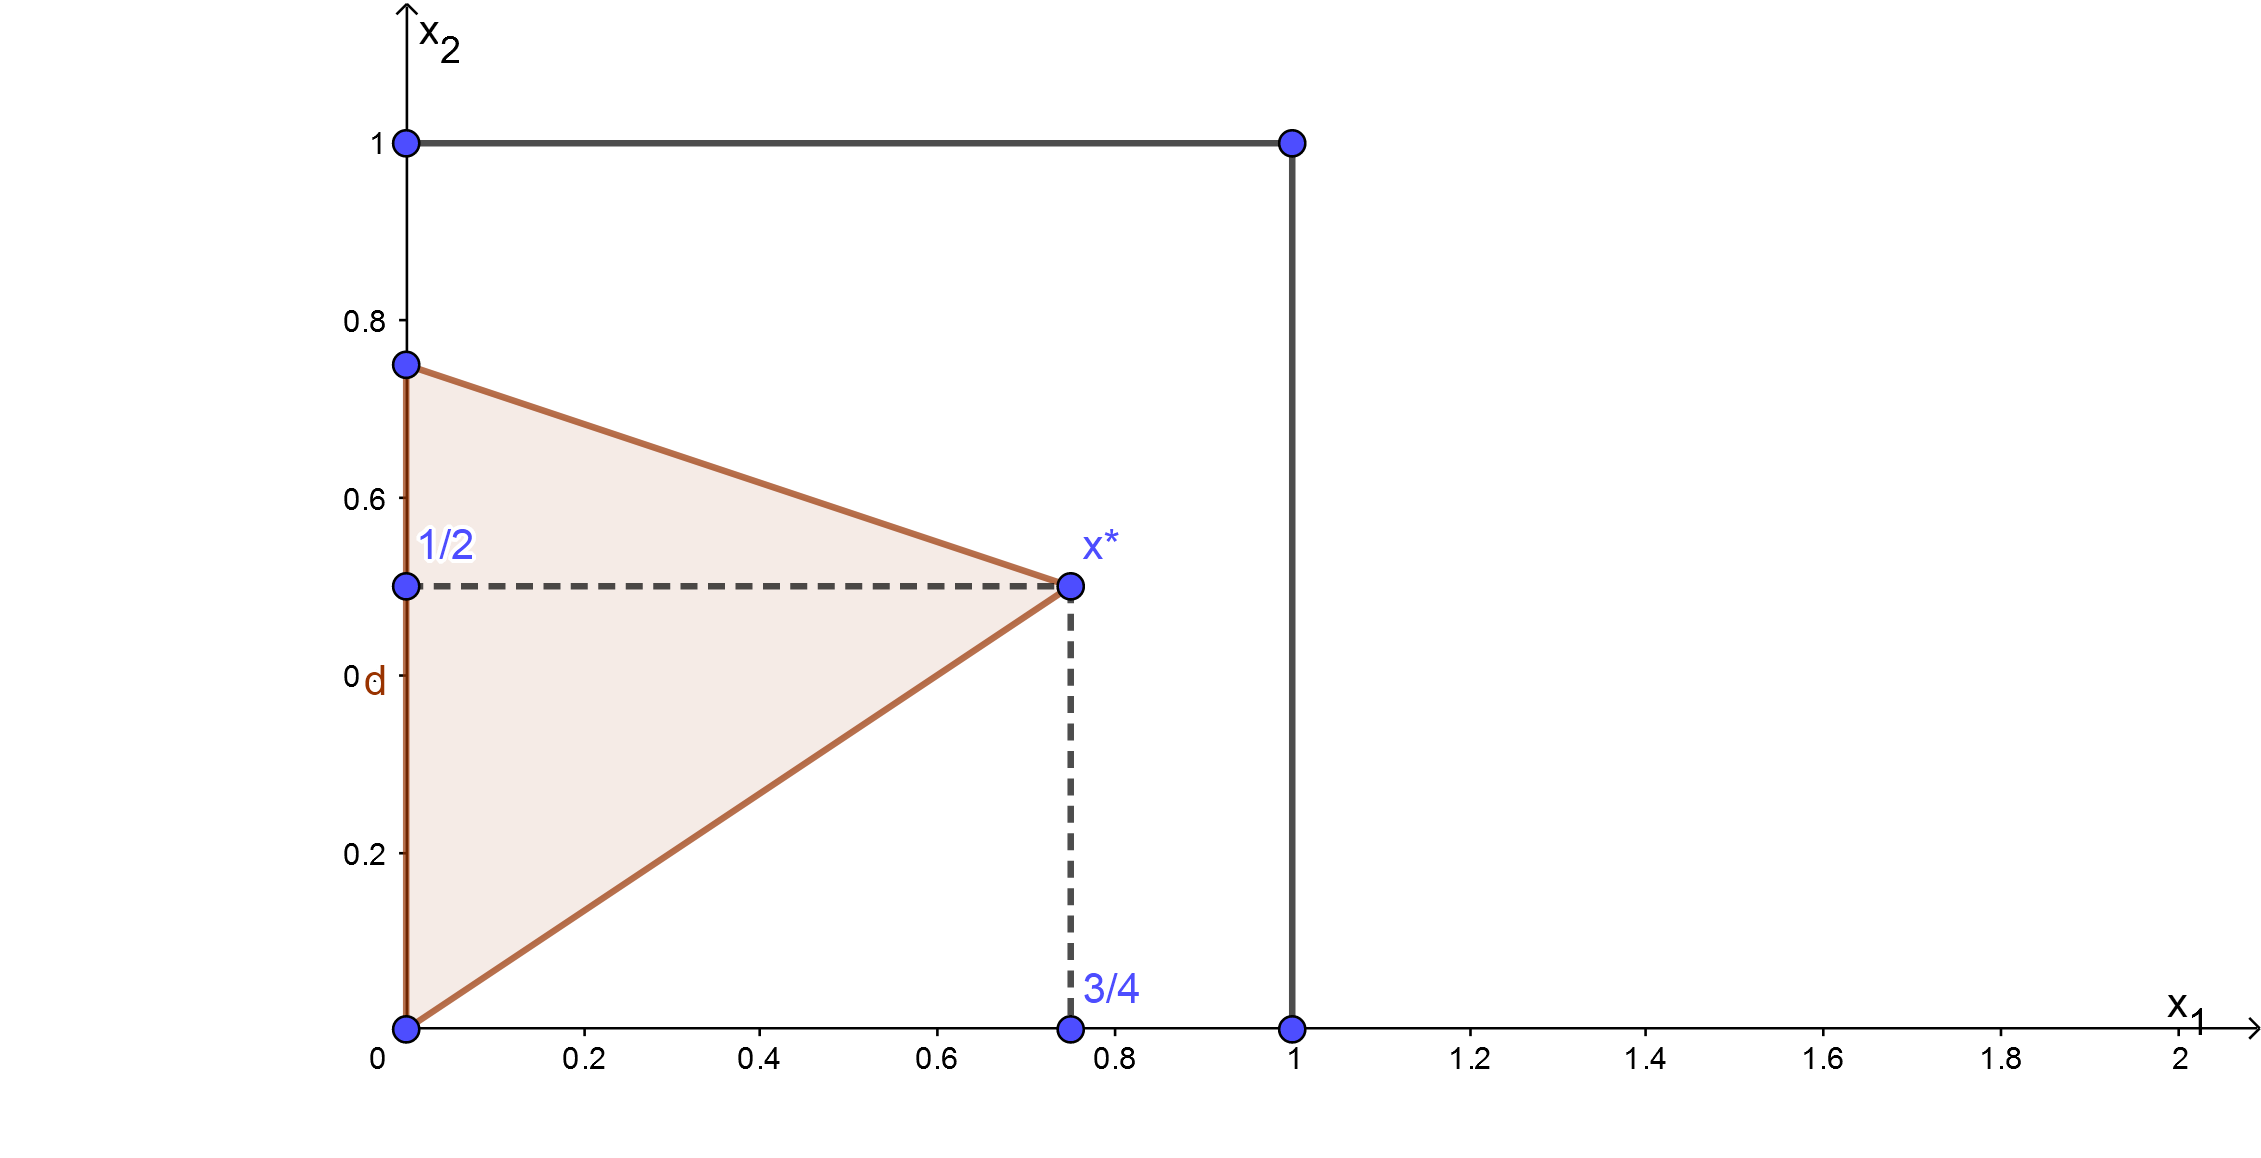
\includegraphics[scale=4]{dw2.png}
 	\caption{Grafička interpretacija problema. Optimalno rješenje je označeno sa $x^*$. }
 	\label{fig:dw1}
 \end{figure}
 
 Prije nego što na ovom problemu ilustrujemo upotrebu DW dekompozicije, riješimo problem na neki od (u ovom slučaju) bržih načina. Ako problem predstavimo grafički (Slika~\ref{fig:dw1}), vidimo da je dopustivi skup osjenčeni trougao, a da se maksimalna vrijednost funkcije cilja dostiže u vrhu $(\frac34, 
 \frac12)$ tog trougla, odnosno,

    \begin{equation}
 z^* = \frac 34,\qquad \textnormal{za}\ x^*=\left(\begin{array}{c}
 	\frac34\\
 	\frac12
 \end{array}\right).
 \end{equation}
 
 Formirajmo sada polaznu konfiguraciju za primjenu DW dekompozicije.
 
 Skup $X$ je politop koji ima četiri tjemena:
 
 $$   
 x^{(1)}=\left(\begin{array}{c}
 		0\\
 		0
 	\end{array}\right),\  x^{(2)}=\left(\begin{array}{c}
 	1\\
 	0
 \end{array}\right),\  x^{(3)}=\left(\begin{array}{c}
 0\\
 1
\end{array}\right) \textnormal{i}\ x^{(4)}=\left(\begin{array}{c}
1\\
1
\end{array}\right)
$$
 
 Zapišimo i polazni problem u kompaktnijem obliku, odnosno
 
 $$
 A = \left(\begin{array}{cc}
 	1 & 3 \\
 	2 & -3
 \end{array}\right) \ b=\left(\begin{array}{c}
 \frac 9 4\\
 0
\end{array}\right)\ c=\left(\begin{array}{c}
1\\
0
\end{array}\right),
 $$
 
 pa polazni problem možemo napisati kao
    \begin{equation}
 	\begin{aligned}\label{primjer:dw2}
 		&\max\ c^Tx\\
 		&\mbox{t.d.}\\
 		  &Ax\leqslant b\\
 		&x \in X
 	\end{aligned}
 \end{equation}
Na osnovu teoreme o reprezentaciji, svako rješenje $x \in X$ možemo zapisati kao

$$\begin{aligned}
&x = \sum_{j=1}^4\lambda_j x^{(j)}\\
&\sum_{j=1}^4\lambda_j=1\\
&\lambda_1,\lambda_2,\lambda_3,\lambda_4\geqslant 0
\end{aligned}$$
 Preformulacijom problema~(\ref{primjer:dw2}) dobijamo
 
     \begin{equation}
 	\begin{aligned}\label{primjer:dw3}
 		&\max\   \sum_{j=1}^4(c^T  x^{(j)})\lambda_j\\
 		&\mbox{t.d.}\\ 
 		 &\sum_{j=1}^4 (A  x^{(j)})\lambda_j\leqslant b\\
 		&\sum_{j=1}^4\lambda_j = 1\\
 		&\lambda_j\geqslant 0,\ j = 1,\ldots,4
 	\end{aligned}
 \end{equation}
 Odnosno, nakon sređivanja 
      \begin{equation}
 	\begin{aligned}\label{primjer:dw4}
 		&\max \  \lambda_2+\lambda_4\\
 		&\mbox{t.d.}\\
 		 &\left(\begin{array}{c}
 			1\\
 			2
 		\end{array}\right)\lambda_2+\left(\begin{array}{c}
 		3\\
 		-3
 	\end{array}\right)\lambda_3+\left(\begin{array}{c}
 	4\\
 	-1
 \end{array}\right)\lambda_4\leqslant \left(\begin{array}{c}
 			\frac 9 4\\
 			0
 		\end{array}\right)\\
 		&\sum_{j=1}^4\lambda_j = 1\\
 		&\lambda_j\geqslant 0,\ j = 1,\ldots,4
 	\end{aligned}
 \end{equation}

Da bismo u ograničenjima izbjegli znak $\leqslant$ u prva dva ograničenja, dodajmo modelu dvije izjednačavajuće promjenljive $s_1$ i $s_2$, te model zapišimo kao
      \begin{equation}
	\begin{aligned}\label{primjer:dw5}
		&\max\   \lambda_2+\lambda_4\\
		&\mbox{t.d.}\\
		  &\lambda_2+3\lambda_3+4\lambda_4+s_1=\frac 94\\
		&2\lambda_2-3\lambda_3-\lambda_4+s_2=0\\
		&\sum_{j=1}^4\lambda_j = 1\\
		&\lambda_j\geqslant 0,\ j = 1,\ldots,4\\
		&s_1,s_2\geqslant 0
	\end{aligned}
\end{equation}

Sada se može inicijalnizovati RMP, biranjem dopustive baze.

Izabraćemo promjenljive $\lambda_1, s_1$ i $s_2$ kao inicijalne bazne promjenljive. Pošto  promjenljive $\lambda_2,\lambda_3$ i $\lambda_4$ ne egzistiraju u podproblemu,  RMP izgleda ovako
      \begin{equation}
	\begin{aligned}\label{primjer:dw6}
		&\max\   0\\
		&\mbox{t.d.}\\  
		&s_1=\frac 94\\
		&s_2=0\\
		&\lambda_1 = 1\\
		&\lambda_1,s_1,s_2\geqslant 0
	\end{aligned}
\end{equation}
Posljednji problem se trivijalno rješava. Funkcija cilja ima vrijednost 0, a vrijednost promjenljivih se direktno očitavaju iz ograničenja. Ispitajmo sada optimalnu vrijednost dualnih promjenjivih, dakle $y$ i $\alpha$ uz pomoć simpleks tabele problema (\ref{primjer:dw6}). Ona izgleda ovako
\begin{center}

\begin{tabular}{c|cccc}
	       &$s_1$  & $ s_2$   & $\lambda_1$ &  \\
 $s_1$	   &  1  &   0      &   0         &  $\frac{9}{4}$ \\
  $s_2$	  &  0  &    1     &   0         &  0             \\
$\lambda_1$	  &  0  &    0     &   1         &  1   \\ \hline
	$z$   & 0  &    0     &   0         &  0
\end{tabular}
\end{center}
 
Posmatrajmo sada dualni problem problema~(\ref{primjer:dw3}). Označimo sa $y_1$, $y_2$ i $\alpha$ promjenljive dualnog problema. Kako imamo optimalnu simpleks tabelu, vrijednost optimuma dualnih promjenjivih jednaka je odgovarajućim koeficijentima doprinosa (posljednji red tabele), pa je $y_1 = 0 = y_2 = \alpha$. 

%Za dalje razmatranje biće nam potrebna  Tabela~\ref{tbl:dw1}, koju ćemo popunjavati u iterativnom procesu.


\emph{Iteracija 1.} 
Konstruišemo CG problem sa
\begin{align}\label{eq:cg-1}
	 \max_{x \in X} (1, 0)^T x + 0 - (0, 0) \left(\begin{array}{cc}
	 	1 & 3 \\
	 	2 & -3
	 \end{array}\right)  x = \max_{x \in X} x_1. 
\end{align} 
Optimalna vrijednost problema (\ref{eq:cg-1}) je jednaka $\hat{z}=1$, i dostiže se, recimo, u ekstremnoj tački $ x^{(2)}= (1, 0)^T.$ Kako je optimalna vrijednost pozitivna, ulazna kolona za prethodni podproblem postoji, te je treba da odaberemo. Ova kolona (ako posmatramo problem (\ref{primjer:dw5})) će biti data sa 
\begin{align}
     \begin{pmatrix}
     	    c^T  x^{(2)} \\
     	    A x^{(2)}  \\
     	    1     \\
     \end{pmatrix} = \begin{pmatrix}
               1 \\
               1  \\
               2  \\
               1\\
 \end{pmatrix}
\end{align}
Kada pogledamo prethodne vrijednosti kolone i master problem (\ref{primjer:dw5}), jasno je da ona odgovara koeficijentima promjenljive $\lambda_2$. Dakle, prethodna kolona je data u odnosu na $\lambda_2$, ali je sada prebacimo na trenutnu bazu datu sa $s_1, s_2$ i $\lambda_1$, gdje je $B^{-1} =  \begin{pmatrix}
	1 & 0 & 0 \\
	0 & 1 & 0  \\
	0 & 0 & 1  \\
\end{pmatrix}. $ %da bismo dodali potrebnu kolonu za RMP. 
Za to je potrebno izvršiti njenu transformaciju na nove baze čiji su koraci opisani u Tabeli \ref{tbl:dw1}, odakle dobijamo kolonu za dodavanje u RMP


$$	\begin{pmatrix}
	       1 \\
	      1  \\
	      2  \\
	      1\\
	\end{pmatrix}
 $$
 
  \begin{table}\centering
 	\begin{tabular}{|c|c|c|} \hline
 		$\vdots$ & 	$B^{-1}$& $B^{-1}b$ \\
 		\hline
 		$BV$ &	$(y_1,y_2,\alpha)=c^T_B B^{-1}$ & $\overline{z}= c^T_B B^{-1}b$ \\	
 		\hline
 	\end{tabular}\caption{Forma tabele za praćenje vrijednosti u iterativnom procesu DW dekompozicije}\label{tbl:dw1}
 \end{table}
 
 

Ubacimo za trenutak ovu kolonu u prethodnu simpleks tabelu, odakle imamo tabelu

 \begin{center}
 	
 	\begin{tabular}{c|ccccc}
 	                &$s_1$        & $ s_2$   &  $\lambda_1$ & $\lambda_2$   &                \\
 		$s_1$	    &   1      &    0         &   0         &     1         &  $\frac{9}{4}$ \\
 		$s_2$	    &   0      &    1         &   0         &     2         &  0             \\
 		$\lambda_1$ &   0      &    0         &   1         &     1         &  1             \\ \hline
 		$z$         &   0      &    0         &   0         &    -1         &  0
 	\end{tabular}
 \end{center}
Primijetimo da je cijena doprinosa dodate kolone promijenjena sa 1 na -~1, jer je, zbog korištenja tabelarne forme simpleks metoda, optimalna vrijednost problema zapravo -$\hat{z}$, pošto se CG podproblem minimizuje. Sada koristimo novu kolonu kao ulaznu kolonu za transformacije -- u njoj tražimo kandidata za pivota kako smo to i vidjeli u simpleks metodi. Odaberemo element čija je vrijednost $2$ i pivotiramo oko njega. Prvo sve elemente u koloni 2 podijelimo sa 2, te potom izvršimo elementarne transformacije da bi ostali elementi novododate kolone dobili vrijednost nula. Promjenljiva $s_2$ se isključuje iz baze, dok se $\lambda_2$ uključuje u bazu. Na kraju dobijamo (transformisanu) tabelu:

\begin{center}
	
	\begin{tabular}{c|ccccc}
	             	&$s_1$     &    $ s_2$                &  $\lambda_1$   & $s_2$     &                \\
		$s_1$	    &   1      &   -$\frac{1}{2}$         &   0         &     0         &  $\frac{9}{4}$ \\
		$\lambda_2$ &   0      &    $\frac{1}{2}$         &   0         &     1         &  0             \\
		$\lambda_1$ &   0      &    -$\frac{1}{2}$        &   1         &     0         &  1             \\ \hline
		$z$         &   0      &    $\frac{1}{2}$         &   0         &    0          &  0
	\end{tabular}
\end{center} 
Dakle, bazne promjenljive su sada iz skupa $\{s_1, \lambda_1, \lambda_2\}$, koji odgovara baznoj matrici 
$B^{-1} = 
\begin{pmatrix}
	   1 & -\frac{1}{2}    &  0 \\
	   0 & \frac{1}{2}     &  0  \\
	   0 & -\frac{1}{2}    &  1  \\
\end{pmatrix}$.
Na osnovu prethodne simpleks tabele, dobijamo   vrijednosti dualnih promjenljivih iz koeficijenta doprinosa, tj. $y_1 = 0, y_2 = \frac{1}{2}, \alpha = 0$. 


\vspace{5mm}

\emph{Iteracija 2.} Iz prethodnog dobijamo CG podproblem 
\begin{align}
	 \max_{x \in X} (1, 0)^T x - \left(0, \frac{1}{2}\right)\left(\begin{array}{cc}
	 	1 & 3 \\
	 	2 & -3
	 \end{array}\right)  x   - 0 = \max_{x \in X}x_1 - x_1 + \frac{3}{2}x_2 = \max_{x \in X} \frac{3}{2}x_2.
\end{align}
Rješenje ovog problema se lako dobija, tj. optimum se dostiže u, recimo,  tački $x^{(3)}= (0, 1)^T$, dok je optimalna vrijednost jednaka $\hat{z}= \frac{3}{2}$. Kako je $\hat{z} > 0$, treba da odaberemo novu kolonu koja se dodaje u RMP. 
Ova kolona, ako posmatramo problem (\ref{primjer:dw5}), je   data sa 
\begin{align}
	V =   \begin{pmatrix}
		c^T  x^{(3)}\\
		A  x^{(3)}  \\
		1     \\
	\end{pmatrix} = \begin{pmatrix}
		0 \\
		3  \\
		-3  \\
		1\\  
	\end{pmatrix}.
\end{align}

Kada pogledamo prethodne vrijednosti kolone $V$ i master problem (\ref{primjer:dw5}), jasno je da ona odgovara koeficijentima promjenljive $\lambda_3$. Dakle, prethodna kolona je data u odnosu na promjenljivu $\lambda_3$ početnog problema, ali je sada izražavamo preko trenutne baze (podproblema) vektora $s_1, s_2$ i $\lambda_2$. Dakle, nakon množenja kolone sa inverzom baze $B^{-1}$, na osnovu koraka opisanih u Tabeli \ref{tbl:dw1}, sljedeća kolona se dodaje u simpleks tabelu:

\begin{center}
 
  $\begin{pmatrix}
	 -\frac{3}{2}            \\
	 \frac{9}{2}     \\
 	-\frac{3}{2}       \\
	 \frac{5}{2}    \\
   \end{pmatrix}$.
\end{center}
Dakle, dobijamo tabelu 

\begin{center}
 
		\begin{tabular}{c|cccc|c}\vspace{1mm}
		   $s_1$	    &   1      &   -$\frac{1}{2}$         &   0         &   $\frac{9}{2}$          &  $\frac{9}{4}$ \\\vspace{1mm}
		   $\lambda_2$  &   0      &    $\frac{1}{2}$         &   0         &  -$ \frac{3}{2}$         &  0             \\\vspace{1mm}
		   $\lambda_1$  &   0      &    -$\frac{1}{2}$        &   1         &  $\frac{5}{2} $          &  1             \\ \hline\vspace{1mm}
		   $z$          &   0      &    $\frac{1}{2}$         &   0         &   -$\frac{3}{2}$       & 0  
	\end{tabular}
 
\end{center} 
Sada nađimo pivota oko kolone koja je dodana. Kandidati za izlazak iz baze su ili $s_1$ ili $\lambda_2$ dok će mjesto njih ući promjenljiva $\lambda_3$. Kako je $\frac{\frac94}{\frac92}=\frac{1}{2} > \frac{1}{\frac52}=\frac{2}{5}$, imamo da je $\frac{5}{2}$ pivot element. Sada pivotiramo oko tog elementa, tako da se, elementarnim transformacijama po vrstama, kolona transformiše  na kolonu sa svim nulama osim na poziciji pivota, gdje treba da stoji jedinica. Na taj način, simpleks tabela se transformiše u novu simpleks tabelu 

\begin{center}
	
	\begin{tabular}{c|cccc|c}\vspace{1mm}
		$s_1$	    &   1      &    $\frac{2}{5}$          &   -$\frac{9}{5}$       &   0          &  $\frac{9}{20}$ \\\vspace{1mm}
		$\lambda_2$  &   0      &    $\frac{1}{5}$         &   $\frac{3}{5}$        &   0          &  $\frac{3}{5}$             \\\vspace{1mm}
		$\lambda_3$  &   0      &    -$\frac{1}{5}$        &   $\frac{2}{5}$        &   1          &  $\frac{2}{5}$            \\ \hline\vspace{1mm}
		$z$          &   0      &    $\frac{1}{5}$         &  $ \frac{3}{5}$        &   0           & $\frac{3}{5}$
	\end{tabular}
	
\end{center} 
  Pročitamo vrijednost dualnih promjenjivih u posljednjoj vrsti: $y_1 =0, y_2=\frac{1}{5}$ i $\alpha=\frac{3}{5}$.
  
  
  \vspace{5mm}
   \emph{Iteracija 3.} Prema tome, novi CG podproblem je dat sa 
  \begin{align*}
        \max_{x \in X} (1, 0)^T x - (0, \frac{1}{5})\left(\begin{array}{cc}
       	1 & 3 \\
       	2 & -3
       \end{array}\right)  x   - \frac{3}{5} &= \max_{x \in X}x_1  - \frac{2}{5}x_1 + \frac{3}{5}x_2 - \frac{3}{5} \\
       &= \max_{x \in X} \frac{3}{5}x_1 + \frac{3}{5}x_2 - \frac{3}{5}.
  \end{align*} 
Optimalna vrijednost CG podproblema se dostiže u $x^{(4)} = (1, 1)^T$ i ona je jednaka $\hat{z}=\frac{3}{5}$. Kako je $\hat{z}>0$, tražićemo novu kolonu koju treba dodati u podproblem. Ova kolona, ako posmatramo problem (\ref{primjer:dw5}), je   data sa 
\begin{align}
	V =   \begin{pmatrix}
		c^T x^{(4)}\\
		A x^{(4)}  \\
		1     \\
	\end{pmatrix} = \begin{pmatrix}
		1 \\
		4  \\
		-1  \\
		1\\  
	\end{pmatrix}
\end{align}
Kada pogledamo prethodne vrijednosti kolone $V$ i master problem (\ref{primjer:dw5}), jasno je da ona odgovara koeficijentima promjenljive $\lambda_4$. Dakle, prethodna kolona je data u odnosu na promjenljivu $\lambda_4$ početnog problema, ali je sada izražavamo preko trenutne baze (podproblema) vektora $s_1, \lambda_2$ i $\lambda_3$.  Nakon množenja kolone sa inverzom baze 
$B^{-1}= 
\begin{pmatrix}
	 1 &  \frac{2}{5}   & -\frac{9}{5} \\
	 0 &  -\frac{1}{5}  & \frac{3}{5}  \\
	 0 &  -\frac{1}{5}  & \frac{2}{5}  \\ 
\end{pmatrix} $ i na osnovu koraka opisanih u Tabeli \ref{tbl:dw1}, dobijamo da se sljedeća kolona dodaje u simpleks tabelu

\begin{center}
	
	$\begin{pmatrix}
		-\frac{3}{5}            \\
		\frac{9}{5}     \\
		 \frac{2}{5}       \\
		\frac{3}{5}    \\
	\end{pmatrix}$
\end{center}
Dakle, imamo simpleks tabelu 

\begin{center}
	
	\begin{tabular}{c|cccc|c}\vspace{1mm}
		$s_1$	    &   1      &    $\frac{2}{5}$          &   -$\frac{9}{5}$       &  $\frac{9}{5} $        &  $\frac{9}{20}$ \\\vspace{1mm}
		$\lambda_2$  &   0      &    $\frac{1}{5}$         &   $\frac{3}{5}$        &   $\frac{2}{5}$        &  $\frac{3}{5}$             \\\vspace{1mm}
		$\lambda_3$  &   0      &    -$\frac{1}{5}$        &   $\frac{2}{5}$        &   $\frac{3}{5}$         &  $\frac{2}{5}$            \\ \hline\vspace{1mm}
		$z$          &   0      &    $\frac{1}{5}$         &  $ \frac{3}{5}$        &   -$\frac{3}{5}$         & $\frac{3}{5}$
	\end{tabular}
	
\end{center} 
Nađimo sada pivota u dodanoj koloni. Kako je $\frac{\frac{9}{20}}{\frac95} < \frac{\frac25}{\frac35}< \frac{\frac35}{\frac25}$, slijedi da je pivot element $\frac{9}{5}$.  Sada pivotiramo oko tog elementa, tako da se kolona transformiše elementarnim transformacijama po vrstama na kolonu sa svim nulama osim na poziciji pivota, gdje treba da stoji jedinica. Na taj način, simpleks tabela se transformiše u novu simpleks tabelu 
\begin{center}
	
	\begin{tabular}{c|cccc|c}\vspace{1mm}
		$\lambda_4$	 &   $\frac{5}{9}$      &    $\frac{2}{9}$          &   -1       &  1      &  $\frac{1}{4}$ \\\vspace{1mm}
		$\lambda_2$  &   -$\frac{2}{9}$    &   $\frac{1}{9}$        &   1        &   0         &  $\frac{1}{2}$        \\\vspace{1mm}
	    $\lambda_3$  &  -$\frac{1}{3}$     &    -$\frac{1}{3}$      &   1        &   0        &  $\frac{1}{4}$      
		    \\ \hline\vspace{1mm}
		$z$          &   $\frac{1}{3}$     &    $\frac{1}{3}$         &  $0$        &  0         & $\frac{3}{4}$
	\end{tabular}
	
\end{center} 
Iz prethodne tabele pročitamo vrijednost dualnih promjenljivih: $y_1 =  \frac{1}{3}=y_2$, dok je $\alpha=0$. 

\vspace{5mm}

\emph{Iteracija 4.} Na osnovu vrijednosti dualnih promjenljivih, formira se novi CG podproblem
 
	 \begin{align*}
		\max_{x \in X} (1, 0)^T x - \left(\frac{1}{3}, \frac{1}{3}\right)\left(\begin{array}{cc}
			1 & 3 \\
			2 & -3
		\end{array}\right)  x   - 0 &= \max_{x \in X} (x_1  - x_1 ) = 0    
	\end{align*} 
  Iz ovoga zaključujemo da je $\hat{z}=0$, pa iz (\ref{dw8}) slijedi da imamo optimum za početni problem, gdje je optimalna tačka data sa 
\begin{align*}
  	 x^* &= \frac{1}{2}  x^{(2)}+ \frac{1}{4} x^{(3)} + \frac{1}{4} x^{(4)} 
  	     = \frac{1}{2} \begin{pmatrix}
  	     	      1 \\
  	     	      0
  	     \end{pmatrix} +
       \frac{1}{4} \begin{pmatrix}
       	                  0 \\
       	                  1
       \end{pmatrix} +
   \frac{1}{4} \begin{pmatrix}
   	                  1 \\
   	                  1
   \end{pmatrix}\\
   &= \begin{pmatrix}
   	        \frac{1}{2} + 0 + \frac{1}{4} \\
   	        0 + \frac{1}{4} + \frac{1}{4}
   \end{pmatrix} = \begin{pmatrix}
         \frac{3}{4} \\
         \frac{1}{2}
  \end{pmatrix}
\end{align*}
\vspace{1cm} \\

\section{Zadaci}
\begin{enumerate}
	\item % http://motor.ece.iit.edu/ms/benders.pdf
	  	Uz pomoć Benderove dekompozicije riješiti sljedeći MILP problem
	  \begin{align*}
	  	   &\min x + y \\
	  	   &\mbox{t.d.} \\
	  	   & 2x + y \geq 3 \\
	  	   & x \geq 0 \\
	  	   & y \in \{-5, -4,\ldots, 3, 4\}.
   	  \end{align*}
	\item %http://eaton.math.rpi.edu/faculty/Mitchell/courses/matp6620/notesMATP6620/lecture23/23C_benders_egbeamer.pdf
	Uz pomoć Benderove dekompozicije riješiti sljedeći MILP problem
	\begin{align*}
		 &\max 8 y_1 + 9 y_2 + 5 y_3 + 6 y_4 - 15 x_1 - 10 x_2 \\
		 &\mbox{t.d.} \\
		 &y_1 + y_3 \leq 1 \\
		 & y_1 + y_4 \leq 1 \\
		 &y_2 + y_4 \leq 1 \\
		 & -x_1-x_2 \leq -1 \\
		 & y_1 - x_1 \leq 0 \\
		 & y_2 - x_1 \leq 0 \\
		 & y_3 - x_2 \leq 0 \\
		 & y_4 - x_2 \leq 0 \\
		 & y_1,y_2,y_3,y_4,x_1, x_2 \geq 0 \\
		 & x_1, x_2 \in \mathbb{Z}.
	\end{align*}
\item %https://homepages.rpi.edu/~mitchj/matp6640/
%https://personal.eur.nl/birbil/ie606/04_DW_Dec/04_DW_Dec_Octave.html
Uz pomoć DW dekompozicije riješiti sljedeći MILP problem
\begin{align*}
	&\min x_1 - 3 x_2 \\
	&\mbox{t.d.} \\
	& -x_1 + 2x_2 \leq 6 \\
	& x_1 + x_2 \leq 5 \\
	& x_1, x_2 \geq 0.
\end{align*}

\item %https://perso.uclouvain.be/anthony.papavasiliou/public_html/DantzigWolfe.pdf
	Uz pomoć   DW dekompozicije riješiti sljedeći MILP problem
\begin{align*}
	 &\min -4x_1 - x_2 - 6 x_3 \\
	 &\mbox{t.d.} \\
	 & 3 x_1 + 2 x_2 + 4 x_3 = 17 \\
	 & x \in X = \begin{cases}
	 	1 \leq x_1 \leq 2 \\
	 	1 \leq x_2 \\
	    1 \leq x_3 \leq 2. 
	 \end{cases}
\end{align*}
\item %https://homepages.rpi.edu/~mitchj/handouts/egdcmp/ 
    Proučiti opšti slučaj za DW dekompoziciju kada poliedar koji odgovara problemu nije ograničen (u njemu postoji ekstremni zrak). Nakon toga, uz pomoć DW dekompozicije riješiti sljedeći MILP problem
	\begin{align*}
		 &\min x_1 - x_2 - 2 x_3 \\
		 &\mbox{t.d.} \\
		 & x_1 + x_2 + x_3 = 3 \\
		 & x \in X = \begin{cases}
		 	        0 \leq x_1 \leq 2 \\
		 	        0 \leq x_2 \\
		 	        0 \leq x_3 \leq 2. 
		 \end{cases}
	\end{align*}

\end{enumerate}

%TODO... prvo izraziti kolone u odnosu na originalni problem, potom prebaciti u odnosu na bazne vektore, ubaciti u prethodnu simpleks tabelu (baznih vektora), pivotirati tabelu, dobiti novu tabelu, izvuci baze, dualne vrijednosti, formirati novi CG problem. 


 \chapter{Metode za pronalaženje dopustivih rješenja}\label{chp:heuristike}
 
 U prethodnim poglavljima prikazane su najvažnije tehnike za egzaktno rješavanje problema iz oblasti linearnog i cjelobrojnog programiranja. Sa druge strane, u teoriji i praksi se često javljaju i problemi koji se, zbog svoje složenosti i dimenzionalnosti, ne mogu optimalno riješiti uz razuman utrošak memorijskih i vremenskih resursa. Kao što je već i ranije napominjano, u takvim situacijama se postavlja drugačiji cilj u istraživanju, odnosno, traži se dovoljno dobro \emph{dopustivo rješenje} u sklopu resursa sa kojima raspolažemo. Pod dopustivim rješenjem podrazumijevamo ono rješenje koje zadovoljava uslove samog problema, ali ne postoji garancija da je to rješenje i optimalno.
 
 U ovom poglavlju ćemo objasniti neke od tehnika za pronalaženje dopustivih rješenja. Čak i više od toga, prikazaćemo i neke od moćnih optimizacionih tehnika, koje ne garantuju  pronalazak optimalnog rješenja, ali su se u praksi pokazale kao izuzetno koristan alat za rješavanje problema iz oblasti operacionih istraživanja.
 

\section{Pohlepni algoritmi}
 
Pohlepni algoritmi su programska paradigma zasnovana na pristupu da se  rješenje iterativno formira dio po dio (komponenta po komponenta) tako da se naredna komponenta, koja se dodaje u postojeće rješenje, bira 
 po nekom pohlepnom kriterijumu. Preciznije, u svakoj iteraciji se u rješenje uključuje ona komponenta koja donosi najveću korist u odnosu na sve ostale komponente, koje se razmatraju za proširenje  trenutnog parcijalnog rješenja, u nadi da će takvi izbori na kraju dovesti i do kvalitetnog cjelokupnog (kompletnog) rješenja.
 
 %Kod ovakve strategije, u svakom koraku bira se komponenta koja je lokalno najbolji kandidat za proširivanje (parcijalnog) rješenja, u nadi da će takvi izbori na kraju dovesti i do kvalitetnog globalnog rješenja.
 
 Osnovna strategija pohlepnih algoritama isključuje ,,vraćanje'' na neko prethodno (parcijalno) rješenje, odnosno ne vodi se računa o ,,lošim'' odlukama, koje su eventualno napravljene u prethodnim iteracijama. Zbog toga se podrazumijeva da pohlepni algoritmi imaju polinomijalnu vremensku složenost, što je jedna od najvažnijih osobina ovakvih algoritama.
 
 Zbog relativno jednostavne strategije na kojoj su zasnovani, ali i brzine izvršenja, ovi algoritmi se često koriste i u rješavanju teških optimizacionih problema i najčešće su prva strategija koja se primjenjuje, prije 
upotrebe neke složenije paradigme. 
U nekim situacijama se može pokazati da se optimalno rješenje uvijek može dobiti primjenom pohlepnog algoritma. Primjer takvog problema je \emph{razlomljeni problem jednodimenzionalnog ruksaka}, a u nastavku će biti prikazani još neki važni problemi koji se optimalno rješavaju upravo paradigmom pohlepnih algoritama.

Sa druge strane, većina optimizacionih problema se ne može optimalno riješiti pomoću pohlepnih algoritama. U tim slučajevima, ova paradigma se koristi da bi se u kratkom vremenskom periodu obezbijedila dobra približna rješenja, ili da se konstruiše neko polazno dopustivo rješenje, koje će se kasnije unapređivati naprednijim i složenijim algoritamskim tehnikama. 

U ovoj sekciji razmatramo nekoliko poznatih pohlepnih algoritama:
\begin{itemize}
	\item  \emph{Primov algoritam} za pronalaženje minimalnog pokrivajućeg stabla grafa (eng. minimum spanning tree -- MST);
	\item  \emph{Kruskalov algoritam} za pronalaženje MST;
	\item  \emph{Dajkstrin algoritam} za pronalaženje najkraćih puteva u grafu;
	\item  Pohlepni algoritam za rješavanje problema \emph{najdužeg zajedničkog podniza}, za proizvoljan skup stringova u ulazu.
\end{itemize}


\subsection{Algoritmi za pronalaženje MST}

Definišimo prvo pojam pokrivajućeg stabla, pa potom i minimalnog pokrivajućeg stabla.

Neka je dat težinski graf $G=(V,E)$. Svaku težinu grane $(u,v) \in E $ u grafu $G$, označimo sa $w(uv)$. 
\begin{definition}
  Stablo $T =(V_1, E_1)$ je pokrivajuće za graf $G=(V,E)$ akko
  $V_1 = V$ i $E_1 \subseteq E$. Pokrivajuće stablo $T$ grafa $G$ sa minimalnim zbirom težina svojih grana, tj. 
  $\sum_{e \in E_1} w(e)$, se naziva minimalno pokrivajuće stablo (MST) grafa $G$. 
\end{definition}

MST ima primjene u različitim oblastima teorije i prakse. Izdvajamo neke od njih.
\begin{enumerate}
 \item[($i$)] Dizajniranje mreža (npr. telefonske mreže), gdje je do svakog domaćinstva, koje je predstavljeno čvorom grafa, potrebno obezbijediti liniju, tako da se, na kraju, u mrežu povežu sva domaćinstva, uz minimalnu potrošnju materijala potrebnog za kreiranje infrastrukture mreže;
 \item[($ii$)] Aproksimacija drugih teških optimizacionih problema, kao što je problem trgovačkog putnika (TSP), gdje je potrebno naći najkraću konturu koja posjećuje sve čvorove tačno jednom u (težinskom) grafu. Primijetimo da su putevi generisani iz ovakvih kontura (brisanjem jedne od grana konture) takođe MST. Težina ovako dobijenog rješenja MST je manja nego težina rješenja TSP posmatranog grafa, jer je riječ o minimizaciji nad većim skupom rješenja. Na ovaj način  se može pokazati da nalazak MST-a u težinskom grafu aproksimira nalazak TSP-a (nad euklidskim težinskim grafovima).
 \item[($iii$)] Klaster analiza, konkretno za $k$-klaster problem, se može posmatrati kao problem nalaženja MST-a, a potom brisanja $k-1$ najskupljih grana iz MST rješenja. 
 \end{enumerate}

\subsubsection{Primov algoritam} 

Primov algoritam je jedan od osnovnih algoritama koji se, zbog svoje važnosti, ali i jednostavnosti, izučava u teoriji algoritama.  Navešćemo ključne korake algoritma, bez detaljnije analize validnosti algoritma. Algoritam se sastoji od sljedećih koraka:

\begin{enumerate} 
	\item Kreirati skup \emph{mstSkup}=$\emptyset$ da bi se pratili svi čvorovi koji su već uključeni u MST. 
	 \item Dodijeliti vrijednost svakom čvoru u ulaznom grafu: inicijalizovati vrijednosti na +$\infty$.   Dodijeli vrijednost  0 za čvor koji se prvi ubacuje u MST. 
	Ideja dodjele vrijednosti čvorovima koji još nisu prisutni u skupu MST je u efikasnom odabiru grane minimalne težine, koja treba da se doda u trenutno parcijalno rješenje. %Dakle, ažurirane vrijednosti težina grana pomažu da se u razmatranje uključe upravo one  grane spajaju jedan čvor koji je već uključen u MST i jedan čvor koji nije uključen u MST.  
	\item Dok god \emph{mstSkup} ne uključi sve čvorove iz $V$, ponavljamo sljedeće korake: 
	\begin{itemize} 
		\item Izabrati čvor $u\notin\emph{mstSkup} $ sa minimalnom vrijednošću (pohlepni korak); 
		 \item \emph{mstSkup} = \emph{mstSkup}$\cup \{u\}$ (proširivanje parcijalnog rješenja);
		 \item Ažurirati vrijednosti svih susjeda čvora $u$ na sljedeći način:
		      Za svaki susjed $v$, ako je težina grane $uv$ manja od
		              trenutne vrijednosti za $v$, dodijeliti  čvoru $v$ vrijednost $w(uv)$. 		    
	        
	 \end{itemize}
 \end{enumerate}


 \emph{Vremenska složenost}. Ako se za predstavljanje grafa koristi lista susjedstva, složenost algoritma je $O(|V|^2)$. Ako  koristimo prioritetni red za nalaženje grane minimalne težine, dobijamo složenost od $O( |E| \log(|V|))$. 



\subsubsection{Kruskalov algoritam}
 
Kruskalov algoritam radi po principu izbora grana na osnovu njihove težine, gdje se u svakom koraku koristi pohlepna strategija da se bira odgovarajuća grana najmanje težine.
Koraci algoritma su sljedeći. 
 

\begin{enumerate} 
	
	\item Sortirati sve grane polaznog grafa u neopadajućem poretku; neka je tako formirana lista $S$ svih grana u grafu.
	\item Postaviti $\emph{mstSkup} = \emptyset$. 
	\item Odabrati najlakšu granu iz skupa $S$ (pohlepni korak). Provjeriti da li se formira ciklus pri dodavanju grane u skup grana koje su do sada ubačene u skup \emph{mstSkup}; Ako to nije slučaj, ubaciti granu u trenutni skup \emph{mstSkup}. 
	\item Iz liste $S$ ukloniti odabranu granu;
	\item Ponoviti korake 3 i 4, redom, dok se ne doda tačno $|V|-1$ grana u \emph{mstSkup}.
\end{enumerate} 

 \emph{Vremenska složenost}. Kruskalov algoritam se izvršava u $O(|E|\log |E|)$ ili $O(|E|\log |V|)$ vremenu. Sortiranje grana uzima $O(|E| \log|E|)$ vremena. Potom, za svaku granu 
se primjenjuje operacija nalaženja i dodavanja grane u skup \emph{mst}. Ove dvije operacije se izvršavaju u $O(\log |V|)$ vremenu. Dakle, ukupno vrijeme izvršavanja algoritma je $O(|E|\log |E| + |E|\log |V|)$.   Kako je $|E|=O(|V|^2)$, dobijamo složenost $O(|E| \mathrm{log}(|V|))$. 

\subsection{Dajkstrin algoritam}

Ovaj algoritam se koristi za pronalaženje najkraćih puteva u grafu i sličan je Primovom algoritmu. Generiše se tzv. SPT (eng. \emph{shortest path tree}) sa datim korjenim čvorom $s$, tako  što se formiraju dva disjunktna skupa čvorova, jedan koji sadrži čvorove uključene u SPT, dok su u drugom svi ostali čvorovi. 


Inicijalno, svim čvorovima, osim korjenog, je dodijeljena vrijednost beskonačno, tj. $dist[u]=\ +\infty, \forall u \in V\setminus \{s\}$, $dist[s]=0$. 

Neka je $Q = V$.  
U svakom koraku algoritma nalazimo čvor $u$ koji je u skupu $Q$ sa minimalnom udaljenošću \emph{dist} od korjenog čvora $s$. Zatim se posmatraju njegovi susjedi, te težine grana koje polaze od čvora $u$. U slučaju da je zbir vrijednosti vrijednosti $dist[u]$  i težine grane $w(u,v)$ manja od trenutne vrijednosti $dist[v]$, vrijednost $dist[v]$ se ažurira, jer je nađen novi najkraći put od $s$ od $v$.  Čvor $u$ se zatim izbacuje iz skupa $Q$. Algoritam nastavlja sa istim koracima dok god $Q \neq \emptyset$. 

Svi koraci algoritma su dati u Algoritmu~\ref{alg:dijkstra-algorithm}. Nakon završetka algoritma, vrijednosti $dist$[$u$] odgovaraju težini najkraćeg puta od korjenog čvora $s$ do čvora $u$. 


\begin{algorithm}[!ht]
	\begin{algorithmic}[1]
		\FOR{ svaki čvor $v \in V$:} 	%// Inicijalizacija  
	      	\STATE   $dist[v] \gets +\infty$ 	%// Inicijalne udaljenosti od korjenog cvora $s$
		    \STATE $previous[v] \gets null$ 	%// čvor prije u optimalnoj stazi
		\ENDFOR
		\STATE	$dist[s] \gets 0$ 	 
		\STATE	$Q \gets V(G)=V$
		\WHILE{$Q \neq \emptyset$} 	 
		\STATE $u \gets$ čvor iz $Q$ sa najmanjom vrijednošću $dist$
		\STATE $Q \gets Q \setminus \{u\}$
		\FOR{ sve susjede $v$ od $u$}  
		\STATE $temp \gets dist[u] + w(u, v)$
		\IF{$temp < dist[v]$}
		\STATE  $dist[v] \gets temp$
		\STATE $previous[v] \gets u$ 
		\ENDIF
		\ENDFOR
		\ENDWHILE
		\STATE	\textbf{return} $previous$ 
	\end{algorithmic}
    		\caption{Dajkstra($G,s $)}\label{alg:dijkstra-algorithm}
\end{algorithm}

\emph{Vremenska složenost}.  Implementacija Algoritma~\ref{alg:dijkstra-algorithm} ima vremensku složenost $O(|V|^2)$. Ako je graf predstavljen listom susjedstva, i skup $Q$  je implementiran kao binarni hip, 
složenost se redukuje na $O(|E| \cdot \log |V|)$.

Napomenimo da Dajkstrin algoritam ne radi sa grafovima koji imaju negativne težine (pogledati  liniju 12).  Za ovakve grafove,  primjenjuje se Bellman–Ford-ov algoritam koji je baziran na dinamičkom programiranju. Njega ne pominjemo   u ovoj knjizi, ali čitaocu preporučujemo da se, koristeći literaturu ili internet, upozna i sa ovim važnim algoritmom.  %, o kojem ćemo nešto više reći u narednim sekcijama.


\subsection{Razlomljeni problem jednodimenzionalnog ruksaka}\label{sec:frkacruksak}

\begin{definition}
  Neka je dato $n$ proizvoda sa svojim  težinama i vrijednostima, 
  te ruksak čiji je kapacitet $W>0$. \emph{Razlomljeni problem jednodimenzionalnog ruksaka} podrazumijeva odabir proizvoljnih dijelova proizvoda koji se stavljaju u ruksak, tako da vrijednost proizvoda u ruksaku bude što veća, ali da se pri tom ne naruši ograničenje vezano za ukupan kapacitet ruksaka.
\end{definition}
U 0-1 problemu ruksaka, koji će biti razmatran i u Primjeru~\ref{primjer:01ruksak},  ne dopušta se dijeljenje proizvoda. Dakle, ili se uzima cijeli proizvod (1) i stavlja u ruksak, ili se uopšte ne uzima (0). U  razlomljenom problemu ruksaka, svaki proizvod pored svoje težine i vrijednosti,  može da se podijeliti na proizvoljne dijelove (recimo dopušteno je da se uzme   pola od ukupne količine proizvoda i ubaci u ruksak). Primjeri takvih proizvoda bi bili mlijeko, so, šećer, itd. Efikasno rješavanje ovog problema se izvodi primjenom pohlepnog algoritma na sljedeći način.
\begin{enumerate}
	\item Računaju se odnosi vrijednost/težina za svaki proizvod, te se proizvodi  sortiraju na osnovu tih vrijednosti, u opadajućem poretku. 
	   \item Sve dok ruksak nije potpuno napunjen ponavljamo sljedeći postupak:
	   	\begin{itemize}
	   		\item  Iz liste sortiranih proizvoda, uzmemo onaj proizvod kod koga je izračunati odnos najveći;.
	   		\item  Dodamo  ga u ruksak u maksimalnoj količini, vodeći računa da ne narušimo kapacitet ruksaka.
	   		\item Uklonimo taj proizvod iz liste.
	   	\end{itemize} 
	   
\end{enumerate}
Može se pokazati sljedeća teorema. 

\begin{thm}
      Prethodno opisan pohlepni algoritam za razlomljeni problem jednodimenzionalnog ruksaka uvijek nalazi optimalno rješenje.
\end{thm}
\subsection{Pohlepni pristup za rješavanje LCS problema}

String definišemo kao niz karaktera nad konačnom azbukom $\Sigma$.
\begin{definition} 
Problem najdužeg podniza (eng. \emph{Longest common subsequence} -- LCS), je problem koji u ulazu uzima $n$ stringova proizvoljne dužine. Cilj je da se pronađe string maksimalne dužine koji je zajednički podniz za sve stringove iz ulaznog skupa stringova. 
\end{definition}


\begin{primjer}\label{primjer:lcs}
 Neka su u ulazu data tri stringa dužine šest: $$S = \{  \texttt{abbccb}, \texttt{abccab}, \texttt{abbbcb}   \}.$$  Rješenje problema je $s=\texttt{abcb}$. Primijetimo da je $s$ podniz za sva tri stringa iz $S$, a može se (direktno) provjeriti da je to najduži takav string. 
 \end{primjer}
 
 Ovaj problem se može riješiti u $O(n^m)$ vremenu uz pomoć dinamičkog programiranja, gdje je $n$ dužina najdužeg stringa u ulazu, a $m$ broj stringova u ulazu. Specijalno, za  $m=2$, problem je rješiv u $O(n^2)$ vremenu. Za proizvoljno $m$ i $n$, ovaj problem je NP-težak.  


Jedan od najjednostavnijih pristupa za rješavanje ovog problema je  \emph{pohlepni pristup}, tzv. \emph{Best-Next} (BN) heuristika. Prije nego što navedemo detalje algoritma, uvedimo nekoliko definicija i oznaka koje će biti korištene u konstrukciji ovog algoritma. 

Za cjelobrojni vektor $p^L = (p^L_1,\ldots, p^L_m)$, definišemo kolekciju stringova
$S[p^L] = \{s_i[p^L_i, |s_i|] \mid i=1,\ldots,m\}$, gdje $|s|$ označava dužinu stringa $s$, a $s[x,y]$ podstring stringa $s$ koji počinje od karaktera na poziciji $x$, a završava sa karakterom na poziciji $y$. Konvencija je da se indeksi u stringu numerišu krenuvši od 1. Dakle, $s= [1, |s|]$ za svaki string $s$. Primjera radi, za (pozicioni) vektor $p^L=(2,3,4)$ i skup $S$ iz Primjera~\ref{primjer:lcs} imamo $S[ p^L] = \{ s_1[1, |s_1|], s_2[2, |s_2|], s_3[3, |s_3|]  \}= \{ \texttt{bbccb}, \texttt{ccab}, \texttt{bcb}\}$. 

 
Dalje, sa $p^L_{i,a}$ definišemo poziciju prvog pojavljivanja karaktera $\texttt{a}\in \Sigma$ takav da je $p^L_{i,a} \geq p^L_i$ (ukoliko karakter ne postoji, dodijelimo vrijednost $n+1$). Skup karaktera $\Sigma_{p^L}$ koji se pojavljuju u svakom od stringova (u podproblemu) $S[p^L]$ su dopustive ekstenzije u odnosu na pozicioni vektor $p^L$. 

U konstrukciji pohlepnog algoritma, odredimo  skup dopustivih komponenti i (pohlepni) kriterijum odabira najbolje komponente u svakom koraku algoritma koja se dodaje u postojeće parcijalno rješenje. Inicijalno rješenje $s$ je prazan string, koje je, trivijalno, dopustivo za svaku instancu LCS problema. Ideja se sastoji u iterativnom proširivanju trenutnog rješenja za jedan karakter, spajajući taj karakter sa rješenjem sa desna, dok god je to moguće. Pri tome prošireno rješenje mora uvijek biti zajednički podniz, dakle, dopustivo. Za spajanje stringa i karaktera ćemo koristiti standardni operator ($\cdot$).

 Prema navedenom, krenemo sa pozicijom $p^L = (1, \ldots, 1)$ koja odgovara čitavom skupu $S=S[p^L]$ i praznim stringom $s =\varepsilon$ kao inicijalnim rješenjem. Dalje, da bismo očuvali dopustivost rješenja kada se rješenje proširi za jedan karakter, za komponente rješenja $\Sigma_{p^L}$ ćemo uzeti sve karaktere koji se nalaze u svim stringovima iz $S=S[p^L]$, dakle u sufiks stringovima u odnosu na odgovarajuće pozicije vektora $p^L$. Na taj način,  ekstenzija $s = s \cdot x$  će za bilo koji $x \in \Sigma_{p^L}$ dati dopustivo LCS rješenje. Među karakterima iz $\Sigma_{p^L}$ treba odabrati (lokalno) najboljeg kandidata za proširivanje rješenja. Treba imati na umu da se kandidat $x\in \Sigma_{p^L}$ može pojaviti na nekoliko pozicija u svakom stringu iz $S=S[p^L]$. Kako ne želimo ekstenzije koje vode ka podoptimalnim rješenjima, za karakter $x$ biramo onaj sa pozicijama pojavljivanja koje su najbliže početku svakog od stringova iz $S=S[p^L]$, dakle na pozicijama $p^L_{i,a},i=1,\ldots,m$. 

 Ideja konstrukcije pohlepne funkcije $g()$ se sastoji u odabiru onog karaktera za proširivanje rješenja $s$ koji, na neki način, izbacuje najmanji broj karaktera iz dalje pretrage. U našem slučaju,  funkcija $g()$ procjenjuje relativan broj izbačenih karaktera u odnosu na veličinu sufiks stringova. 
 Sljedeći korak se sastoji u ažuriranju prostora pretrage za novi korak. Kako smo proširili rješenje za $x$, nove komponente rješenja koje su dopustive ekstenzije trenutnog rješenja tražimo u skupu (sufiks) stringova $S[p^L_{1,x}+1,\ldots, p^L_{m, x}+1]$. Postupak nastavljamo dok god postoje komponente koje mogu proširiti trenutno rješenje $s$. 


 Da rezimiramo, pohlepni (BN) pristup za rješavanje LCS problema se sastoji od sljedećih koraka.
\begin{itemize}
	\item Polazi se od parcijalnog rješenja koje je prazna niska, $s=\varepsilon$;
	\item Iniciramo pozicioni vektor $p^L \gets (1,\ldots, 1) $;
	\item Dok god jedan od $p^L_i$ nije jednak $n+1$, ponavljamo sljedeće korake: 
	\begin{itemize}
   	     \item $\Sigma_{p^L} \gets$ naći dopustive ekstenzije u $S[p^L]$;
	      \item Od svih karaktera u $\Sigma_{p^L}$, odaberemo onaj koji minimizuje vrijednost funkcije 
	      $$g( p^L,a) = \sum_{i=1}^m\frac{p^L_{i,a} - p^L_i + 1 }{|s_i| - p^L_i + 1 }, a \in \Sigma_{ p^L }.$$
	      Označimo taj karakter sa $a^*$. 
	      \item Ažuriramo: $s \gets  s \cdot a^*$, $p^L_i \gets p^L_{i, a^*} +1, i = 1,\ldots,m.$
    \end{itemize}
\end{itemize}
Algoritam vraća vrijednost $s$. 

Primijetimo da ovakav algoritam ne može da garantuje optimalno rješenje, što je ilustrovano sljedećim jednostavnim primjerom. 

\begin{primjer} Neka su data dva stringa: $s_1 = \texttt{caba}, s_2 = \texttt{bacc}$. Prvo konstatujmo da su sva tri karaktera moguće opcije za proširenje (inicijalno praznog stringa $\varepsilon$). Izračunajmo za svakog od njih odgovarajući $g$-skor. Imamo: $g((1,1), \texttt{a}) = \frac{2}{4} + \frac{2}{4}= 1$, $g((1, 1), \texttt{b}) = \frac{3}{4} + \frac{1}{4}=1,$ $g((1,1), \texttt{c}) = \frac{1}{4} + \frac{3}{4} = 1$. Ovdje dolazi do situacije u kojoj, ukoliko ne postoji dodatni kriterij odlučivanja u slučaju jednakih vrijednosti minimalnog $g$-skora za više karaktera, algoritam nasumično donosi odluku o odabiru karaktera (u zavisnosti od internih koraka u algoritmu i korištenih struktura podataka). 
	Ako bi izabrali $\texttt{c}$ kao karakter koji proširuje trenutno (prazno) rješenje u prvom koraku algoritma, u narednom koraku bi algoritam prekinuo sa radom, jer sufiksi koji preostaju za proširenje rješenja $\texttt{c}$ neće dati niti jedan karakter za naredno proširenje.  Dakle, u tom slučaju algoritam vraća rješenje $\texttt{c}$, koje očigledno nije optimalno. Ako bi izabrali recimo karakter \texttt{b} u prvom koraku, naredni (i jedini mogući) karakter koji proširuje trenutno rješenje je \texttt{a}, pa bi algoritam  u tom slučaju vratio (optimalno) rješenje \texttt{ba}. 
	\end{primjer}

\section{Aproksimativni algoritmi} 
  %https://home.cs.colorado.edu/~srirams/courses/csci5654-fall13/ilpLectures.pdf
  
   Za veliki broj složenih optimizacionih problema u praksi ne postoje efikasni egzaktni algoritmi. Drugim riječima, da bi se takvi problemi egzaktno riješili, potrebno je izdvojiti ogromne vremenske i memorijske resurse. Sa druge strane, većina pohlepnih algoritama, ali i naprednijih heuristika, ne daju nikakvu garanciju  kvaliteta nađenog rješenja. Negdje između egzaktnih i heurističkih algoritama su se pozicionirali \emph{aproksimativni algoritmi}, koji su polinomijalne složenosti i pronalaze dopustiva rješenja uz garanciju  njihovog kvaliteta. 
  
  \noindent Algoritam pripada klasi \emph{aproksimativnih algoritma} ako:
  \begin{enumerate}
  	\item se izvršava u polinomijalnom vremenu;
  	%\item garantuje rješenje koje je blizu optimalnog rjesenja;
  	\item posjeduje garanciju da je pronađeno dopustivo rješenje približno optimalnom rješenju, odnosno garantuje se da je od optimalnog rješenja unutar nekog faktora kvaliteta ($c$), bez ikakvog prethodnog znanja o optimumu.
  \end{enumerate}
  Neka je dat algoritam $\mathcal{A}$, problem $P$ i instanca problema $I$. Sa $\mathcal{A}(I)$ označimo (dopustivo) rješenje koje se dobija kao izlaz algoritma $\mathcal{A}$, dok sa $\mathcal{A}^*(I)$ označimo optimalno rješenje za ulaznu instancu $I$. Pretpostavimo da je riječ o problemu maksimizacije. 
  
  Algoritam $\mathcal{A}$ se naziva \emph{aproksimativni algoritam} problema $P$ ako 
  za bilo koji ulaz (instancu) $I$, $\mathcal{A}$ vraća aproksimativno rješenje $\mathcal{A}(I)$ za $A^*(I)$ u polinomijalnom vremenu. 
  
  Postoji dvije vrste aproksimativnih algoritama:
  \begin{itemize}
  	\item \emph{apsolutni aproksimativni algoritam} -- ako je za svaku instancu problema $P$ ispunjeno
  	$$ |\mathcal{A}(I) - \mathcal{A}^*(I)| \leq c,$$ za neko $c\in \mathbb{R}^+$;
  	\item \emph{relativni aproksimativni algoritam} -- ako je   za svaku instancu problema $P$ ispunjeno
  	$$\frac{\mathcal{A}(I)}{\mathcal{A}^*(I)} \geq c,$$ za neko $c\in (0, 1]$.
  \end{itemize}
  
  %\fixme{Marko, ni meni nije jasno da li se u oba slucaja koristi ovaj termin}
  
 U tom slučaju kažemo da je algoritma $\mathcal{A}$ $c$--aproksimativni algoritam.
 \begin{comment}
 Ovo sam prebacio u zadatak
  U literaturi ili na internetu, čitalac može pronaći primjere problema za koji postoji apsolutni apriksimativni algoritam (na primjer, bojenje planarnog grafa, eng. \emph{Planar graph coloring}), odnosno primjer problema za koji postoji relativni apriksimativni algoritam.
  \end{comment}
  
  
   U nastavku navodimo  (relativne) aproksimativne algoritme za nekoliko poznatih problema kombinatorne optimizacije (eng. combinatorial optimization), podoblasti matematičke optimizacije, u kojoj se  optimalno rješenje traži na diskretnom skupu rješenja. 
  
  \subsection{Aproksimativni algoritmi za problem  minimalnog pokrivanja čvorova}\label{sec:aprokspokrivanjecvorova}
  
    \begin{figure}
  	\centering
  	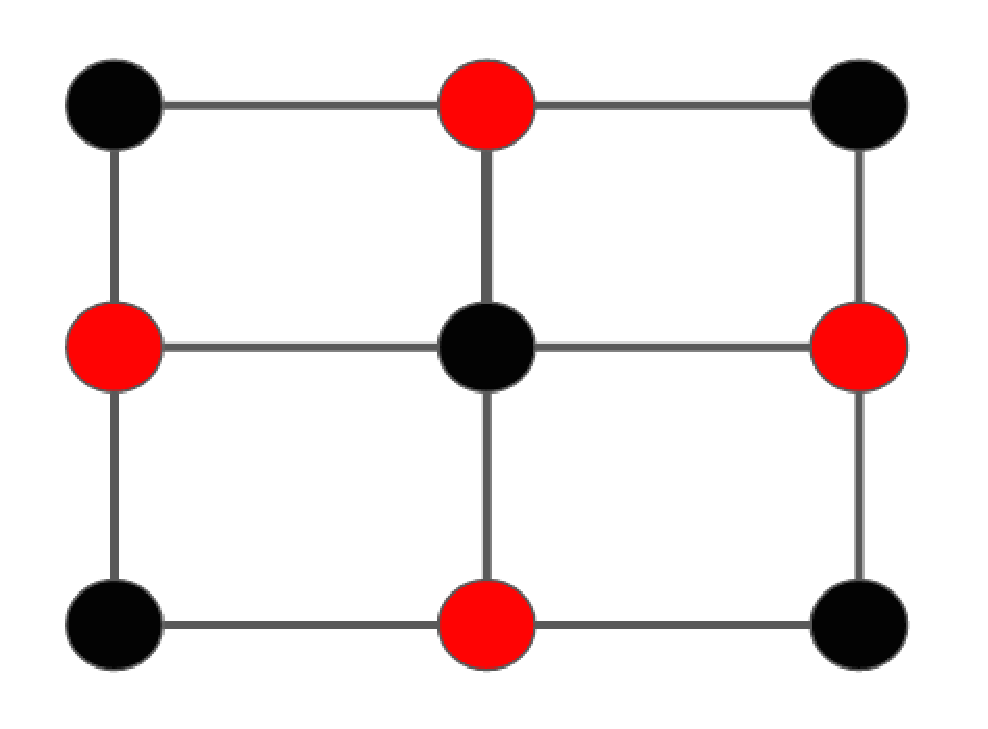
\includegraphics[width=50mm]{vertex-cover.eps}

  	\caption{Primjer pokrivača čvorova grafa.}   	\label{fig:vertex-cover}
  \end{figure}
Definišimo problem minimalnog pokrivanja čvorova.

\begin{definition}
  Neka je dat graf $G=(V,E)$. Potrebno je naći podskup $C\subseteq V$ minimalne kardinalnosti, takav da barem jedan čvor svake grane pripada skupu $C$. 
\end{definition}  
 Skup $C$, koji zadovoljava uslove iz prethodne definicije se naziva \emph{minimalni pokrivač} čvorova grafa $G$. Primjer minimalnog pokrivača jednog grafa je dat na Slici~\ref{fig:vertex-cover} gdje pokrivač uključuje sve čvorove crne boje. 

   Dopustivo rješenje za problem minimalnog pokrivanja čvorova je svaki podskup $C'$, ne obavezno minimalne kardinalnosti, koji sadrži barem jedan čvor svake grane datog grafa.
  
  Posmatrajmo (pohlepni) algoritam za ovaj problem dat Algoritmom~\ref{alg:gridi-vc}. 
  
  %pseudokod algoritma 
  \begin{algorithm}[H] 
  	\begin{algorithmic}[1]
  		\STATE $C \gets \emptyset$
  		\WHILE{$E \neq \emptyset$}
  		\STATE $(u,v)\gets$ bilo koja grana iz $E$
  		\STATE $C \gets C \cup \{u,v\}$
  		\STATE $E \gets $ ukloniti sve grane incidentne sa  $u$ ili $v$ iz grafa $G$
  		\ENDWHILE
  		\STATE \textbf{return} $C$
  	\end{algorithmic}   
   
     \caption{Prvi pohlepni algoritam za problem minimalnog pokrivanja čvorova}
 \label{alg:gridi-vc}
  \end{algorithm}
  
  \noindent Pokazaćemo da je ovo aproksimativni algoritam. Izračunajmo koeficijent aproksimacije $c$ za Algoritam~\ref{alg:gridi-vc}.
  Grane koje se biraju u ovom algoritmu su grane maksimalnog uparivanja ($M$), pa je prema tome, skup $C$ uistinu pokrivač čvorova, prema definiciji uparivanja u grafu. Dalje, jasno je da se algoritam izvodi u polinomijalnom vremenu. Neka je $C^*$ pokrivač koji je rješenje problema. Tada $C^*$ sadrži barem jedan kraj svake grane iz $M$, odakle slijedi $|C^*|\geq |M|$. Dalje, $|C|= 2 \cdot |M| \geq 2 \cdot |C^*|$. Prema tome, ovo je $2$--aproksimativni algoritam za problem pokrivanja čvorova grafa. Jednakost u prethodnoj aproksimaciji se postiže, recimo, za bipartitne grafove $K_{n,n}$. 
 
  
  Posmatrajmo sada i drugi pohlepni Algoritam~\ref{alg:gridi-vc-2} za problem pokrivanja čvorova.  
  
  %pseudokod algoritma 
  \begin{algorithm}[H] 
  	\begin{algorithmic}[1]
  		\STATE $C \gets \emptyset$
  		\WHILE{$E \neq \emptyset$}
  		\STATE  $u \gets \textrm{argmin}_{u \in V(G)} deg(u)$
  		\STATE  $C \gets C \cup \{u\}$
  		\STATE $E \gets$ ukloniti sve grane incidentne sa $u$ u $G$  
  		\ENDWHILE
  		\STATE \textbf{return} $C$
  	\end{algorithmic}
     	\caption{Drugi pohlepni algoritam za problem minimalnog pokrivanja čvorova}
        \label{alg:gridi-vc-2}
  \end{algorithm}
  
  \noindent Izračunajmo aproksimativni faktor Algoritma~\ref{alg:gridi-vc-2} posmatrajući  graf sa Slike~\ref{vertex-coverEx}. 
  
  
  \begin{figure}
  	\centering
  	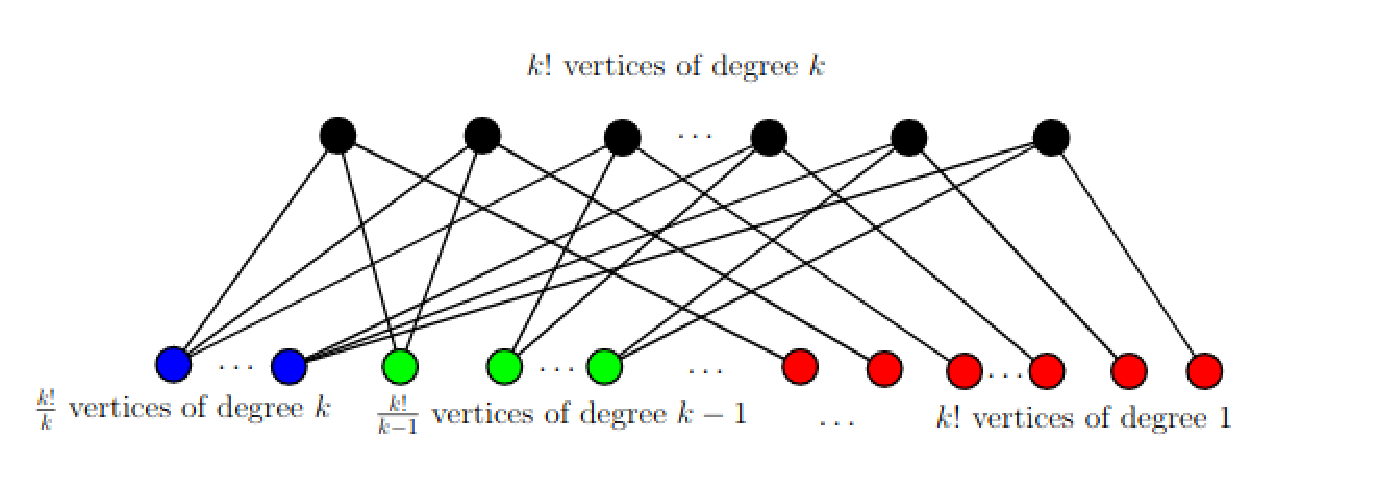
\includegraphics[width=140mm,height=90mm]{vc-2-example.eps}
  	\caption{Specijalan bipartitan graf.} 
  	\label{vertex-coverEx}
  \end{figure}
  
  Optimalno rješenje je podskup čvorova $C^*$, koji se sastoji od svih čvorova sa vrha grafa (obojeni crnom bojom); ukupno ih ima $k!$. Međutim, prateći korake Algoritma~\ref{alg:gridi-vc-2}, dobijamo $$|C| = k!\cdot( 1/k + 1/k-1 + \cdots + 1/2 + 1) \approx k! \cdot \log k.$$  
  Dakle, imamo da je
  $$   |C| \approx \log k \cdot |C^*|.$$ 
  Primijetimo da je u prethodnom zaključku korištena dobro poznata formula 
  
  $$\sum_{j=1}^k \frac1{j} = \log(k)+\gamma+O(1/k),$$
  gdje je $\gamma$ Ojler-Mašeronijeva konstanta (0.577...).
  
  Prema tome, Algoritam~\ref{alg:gridi-vc-2} je $\log k$--aproksimativni, $k \in \mathbb{N}$. 
 
\begin{comment}
 U literaturi, najbolji faktor je $2 - \frac{1}{\sqrt{\log n}}$ (Karakostas, 2009).
  Ono sto se takođe zna (Hastad, 2001) je da ne postoji aproksimativni faktor 
  koji garantuje da je $c < \frac{7}{6}$ (osim ako $P \neq NP$). 
  \end{comment}
  \subsection{Aproksimativni algoritmi za problem trgovačkog putnika}
  
  Za problem trgovačkog putnika nije jednostavno konstruisati efikasan aproksimativni algoritam. Tome svjedoči sljedeća teorema, koja se odnosi na opšti slučaj ovog problema.
  
 \begin{thm}
    Ne postoji polinomijalan algoritam koji može aproksimirati TSP sa  faktorom $c > 1$, osim ako je $P = NP$. 
\end{thm}

Ipak, za neke specifične varijante TSP-a, postoje aproksimativni algoritmi, što ćemo vidjeti u nastavku ovog odjeljka. 
\begin{definition}
  Kažemo da grane grafa zadovoljavaju nejednakost trougla ako za sve različite čvorove $u,v, r$ grafa $G$ vrijedi
  $$ w(u,v) + w(v,r) \geq w(u,r),$$
  gdje su $w(\cdot, \cdot)$ težine grane koja spaja dva čvora.
  \end{definition}
  
  \begin{definition} 
TSP kod koga grane zadovoljavaju nejednakost trougla se naziva \emph{metrički} TSP.
  \end{definition}
  
   Metrički TSP je i dalje NP--težak, ali se aproksimativni algoritam ipak može konstruisati. 

Posmatrajmo \emph{algoritam najbližeg dodavanja} koji aproksimira TSP, dat Algoritmom~\ref{alg:tsp-a1}. 
  
   \begin{algorithm}[!hbt] 
  
  	\begin{algorithmic}[1]
  		\STATE \textbf{Ulaz}: Kompletan težinski graf $G$
  		\STATE \textbf{Izlaz}: Hamiltonova kontura $T$  
  		\STATE $u,v \gets \mbox{argmin}_{uv \in E} w(u,v)$
  		\STATE $S \gets \{u,v\}$
  		\STATE $T \gets uv$
  		\WHILE{$|S| \neq n$}
  		\STATE $(u,t) \gets$ $\mbox{argmin}_{(u,t) \in (V(G)\setminus V(T)) \times V(T)} \{w(u, t)\}$
  		\STATE $ S \gets S \cup \{u\}$ 
  		\STATE $(u, q)\gets$ čvor $q$ slijedi $u$ u  $T$
  		\STATE  $(u,q)$ se izbacuje iz $T$, ubacuje se $(u,t), (t,q)$  // Ažururanje $T$ (rekonstrukcija)
  		\ENDWHILE
  		\STATE \textbf{return} $T$
  	\end{algorithmic}
   	\caption{Prvi aproksimativni algoritam za TSP.}
   	\label{alg:tsp-a1}
  \end{algorithm}

 Ovo je očigledno polinomijalan algoritam. Odredimo aproksimacioni faktor koji se garantuje 
njegovim izvršavanjem. 

Primijetimo da algoritam podsjeća na Primov algoritam. Grane koje se identifikuju algoritmom 
konstruišu MST. Zaključujemo da je cijena konture $T$ barem jednaka koliko i cijena MST u odnosu na iste ulazne podatke. Cijena konture za dva čvora $v_i$ i $v_j$ je $2 \cdot w({v_i,v_j})$ (jer računamo i povratnu granu). Posmatrajmo jednu iteraciju Algoritma~\ref{alg:tsp-a1}, gdje se $T$
proširuje za čvor $t$ koji se ubacuje između čvorova  $u$ i $q$. Povećanje cijene (trenutne) konture $T$ u svakoj iteraciji je $$w({u,t}) + w({t,q})-w({u,q}).$$
Na osnovu nejednakosti trougla imamo $ w({t,q}) \leq w({t,u}) + w({u,q})$. Prema tome, porast cijene konture $T$ u svakoj iteraciji je najviše $ w({t, u}) + w({u,t}) = 2\cdot w({u,t})$. 
Dakle, završna kontura ima cijenu koja dostiže cijenu barem dva puta veću od cijene MST. Prema tome, ovo je 2-aproksimativni algoritam. 

 \noindent Pokušajmo poboljšati aproksimativni faktor Algoritma~\ref{alg:tsp-a1} uz pomoć \emph{algoritma dvostrukog drveta} (eng. double tree algoritma), čije detalje objašnjavamo u nastavku. Prije toga ćemo uvesti nekoliko definicija i teorema od bitnog značaja u konstrukciji algoritma. 
 \begin{definition}
 	  Neka je dat graf $G=(V,E)$. Ojlerova kontura $T^o$ grafa $G$ je kontura $e_1e_2,...,e_me_1$ koja obilazi sve grane grafa $G$. 
 \end{definition}
Vrijedi sljedeća karaketrizacija grafova koji sadrže Ojlerovu konturu. 
\begin{thm}
	 Graf $G$ sadrži Ojlerovu konturu akko je povezan i stepen svakog njegovog čvora paran broj. Takva klasa grafova se naziva Ojlerovom klasom grafova.
\end{thm}
Posmatrajmo sada  Algoritmom~\ref{alg:tsp-a2} i pokažimo da ovim algoritmom  dobijamo 2--aproksimaciju metričkog TSP-a.
 %pseudokod algoritma 
\begin{algorithm}[H] 
	\begin{algorithmic}[1]
		\STATE \textbf{Ulaz}: Kompletan graf $G$
		\STATE \textbf{Izlaz}: Hamiltonova kontura $T$   
		\STATE $mst \gets$  Izračunati MST grafa $G$
		\STATE $mst^{copy} \gets$ Zamijeniti svaku granu u $mst$ sa dvije kopije istog
		\STATE $T^o \gets$ Naći Ojlerovu konturu $T$ u $mst^{copy}$
		\STATE   $T$ $\gets$ Izbaciti duple čvorove iz $T^o$   
		\STATE \textbf{return} $T$ 
	\end{algorithmic}
   	\caption{Drugi aproksimativni algoritam za TSP.}
   	\label{alg:tsp-a2}
\end{algorithm}
   Jasno je da je algoritam polinomijalan i da je dobijeno rješenje dopustivo. 
   
  Neka je $C^*$ cijena optimalne Hamiltonove konture. Tada je cijena MST $\leq C^*$. 
  Lako se vidi da je cijena Ojlerove konture  manja ili jednaka $ 2 \cdot C^*$. Na osnovu nejednakosti trougla, skraćivanje Ojlerove konture (linija 6 u algoritmu) u svrhu dobijanja Hamiltonove konture $T$, ne može da bude veća od 2$C^*$. Dakle, slijedi da je cijena Hamiltonove konture manja ili jednaka $2 C^*$, pa je ovaj algoritam 2--aproksimativni.
  
 
   \begin{figure}[!ht]
 	\begin{subfigure}{.45\textwidth}
 		\centering
 		% include first image
 		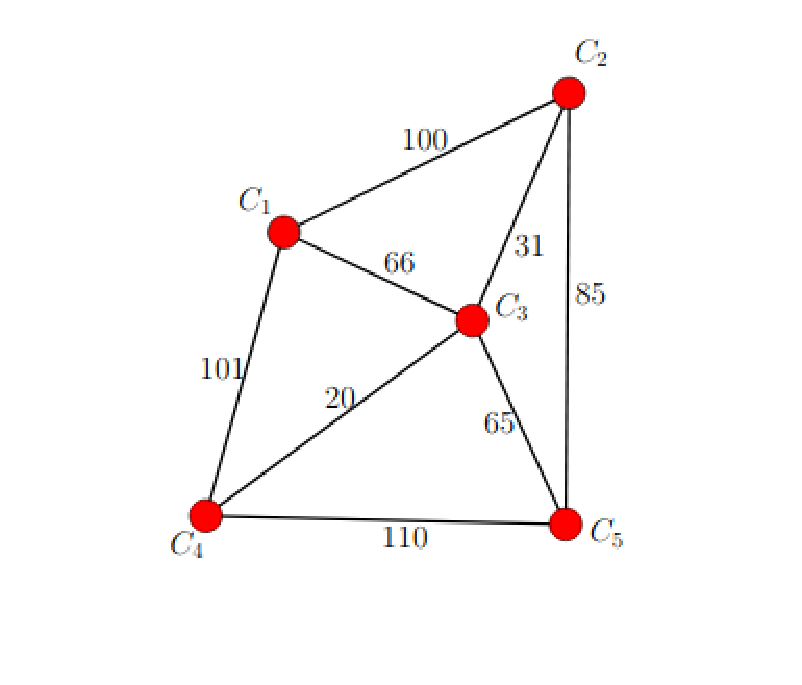
\includegraphics[width=.7\linewidth]{tsp-1}  
 		\caption{Graf $G$.}
 		\label{fig:tsp-1}
 	\end{subfigure}
 	\begin{subfigure}{.45\textwidth}
 		\centering
 		% include second image
 		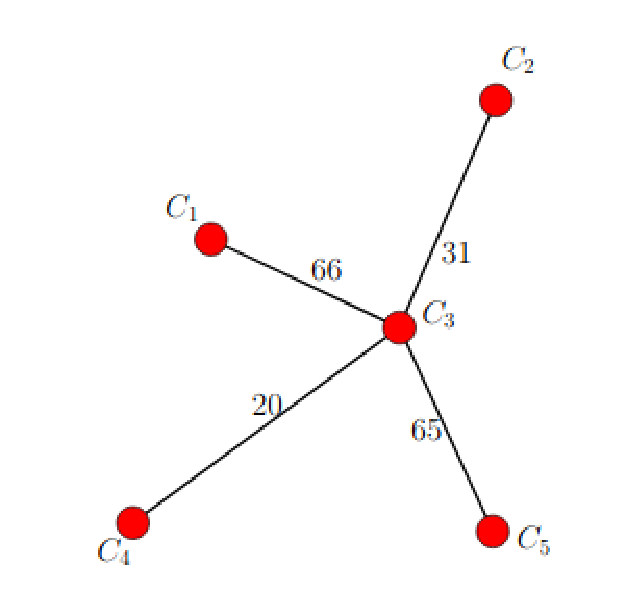
\includegraphics[width=.7\linewidth]{tsp-1a}  
 		\caption{MST grafa $G$}
 		\label{fig:tsp-1a}
 	\end{subfigure}
 
 	\begin{subfigure}{.45\textwidth}
 		\centering
 		% include first image
 		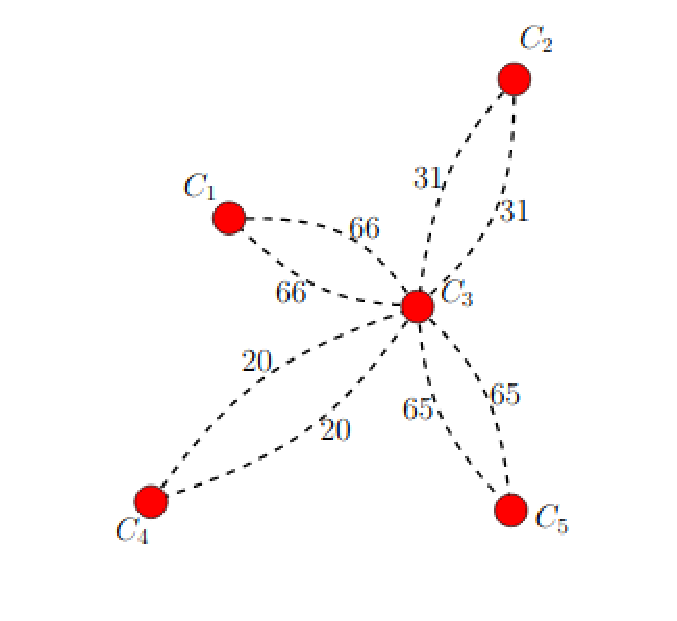
\includegraphics[width=.7\linewidth]{tsp-2a}  
 		\caption{Ojlerova kontura: $C_1 C_3 C_4 C_3 C_5 C_3 C_2 C_3 C_1$.}  
 		\label{fig:tsp-1}
 	\end{subfigure}
 	\begin{subfigure}{.45\textwidth}
 		\centering
 		% include second image
 		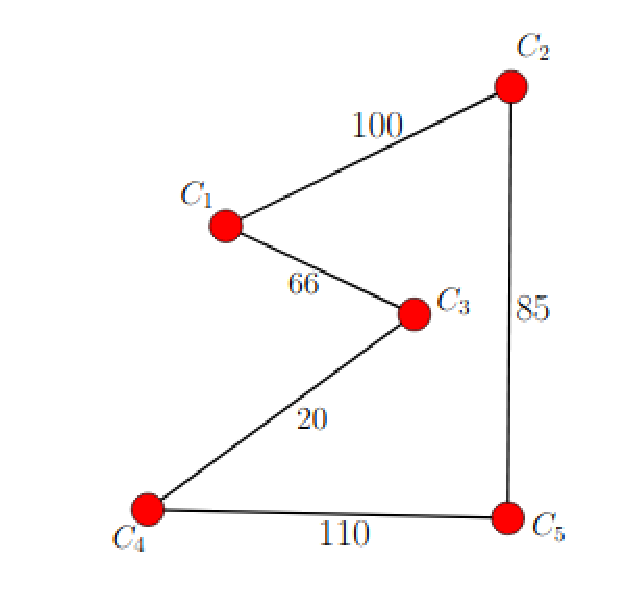
\includegraphics[width=.7\linewidth]{tsp-3a}  
 		\caption{Hamiltonova kontura (ciklus): $C_1C_3C_4C_5C_2C_1$.} 
 		\label{fig:tsp-1a}
 	\end{subfigure}
    \label{fig:tsp-1a1}
    \caption{Koraci u konstrukciji Kristofidjesovog algoritma.}
 \end{figure}



Posmatrajmo još jedan aproksimativni algoritam za TSP koji garantuje aproksimativni faktor od 1.5. Algoritam je poznat pod nazivom \emph{Kristofidesov} algoritam.
Koraci su prikazani Algoritmom~\ref{alg:tsp-a3}.

%pseudokod algoritma 
\begin{algorithm}[H] 

	\begin{algorithmic}[1]
		\STATE \textbf{Ulaz}: Graf $G$
		\STATE \textbf{Izlaz}: Hamiltonova kontura $T$ 
		\STATE $T \gets$ Naći MST grafa $G$
		\STATE $M \gets$ Naći minimalno uparivanje svih čvorova u $T$ neparnog stepena
		\STATE $T' \gets$ Dodamo grane od $M$ u $T$
		\STATE $T^o\gets$ Nađimo Ojlerovu konturu u $T'$
		\STATE $T \gets$ Izbaciti duple čvorove iz $T^o$
		\STATE \textbf{return} $T$
	\end{algorithmic}	
    \caption{Kristofidesov aproksimativni algoritam za TSP.}
    \label{alg:tsp-a3}
\end{algorithm}
  Lako je vidjeti da je ovaj algoritam polinomijalan i da je dobijeno rješenje dopustivo. 
  \begin{thm}
  	  Kristofidesov algoritam ima faktor aproksimacije $c=1.5$.
  \end{thm}
\begin{proof}
  Cijena TSP $C^*$ dostiže najviše cijenu Ojlerove konture, tj.  $C^*\leq cost(T^o) = cost(T) + cost(M)$.  Takođe jasno je da vrijedi $cost(T) \leq C^*$. Pokažimo da je $cost(M) \leq  \frac{C^*}{2}$, što je dovoljno za dokaz teoreme. Primijetimo da u optimalnoj konturi $T$ postoje dva uparivanja: prvi sa čvorovima iz $M$, a drugi za ostale čvorove kojeg označavamo sa $M'$. 
  Kako je $C^* \geq cost(M) \leq cost(M')$ i $cost(M) + cost(M') = cost(T)$, slijedi 
  $2 cost(M) \leq cost(T) \leq C^*$, odakle dobijamo tvrđenje.  
\end{proof} 

U literaturi je pokazano da ne postoji  aproksimacioni algoritam sa faktorom  $c < \frac{220}{219} \approx 1.0045$ (osim ako je $P=NP$). 
 
 
 \subsection{Aproksimativni algoritmi za problem binarnog pakovanja}\label{sec:binpack}
% Zadatak: https://scipbook.readthedocs.io/en/latest/bpp.html

Definišimo \emph{problem binarnog pakovanja}.  
\begin{definition}
    Neka je dato $n$ proizvoda veličine $a_1,a_2,\ldots,a_n$ ($0<a_i \leq 1$). Potrebno je spakovati sve proizvode u pakovanja  jediničnog kapaciteta, tako da je ukupan broj korištenih pakovanja  minimalan.  
\end{definition}

  Primjer jedne instance problema pakovanja je dat na Slici~\ref{fig:bin-packing}.
 

\begin{figure}[H] 
	\centering
	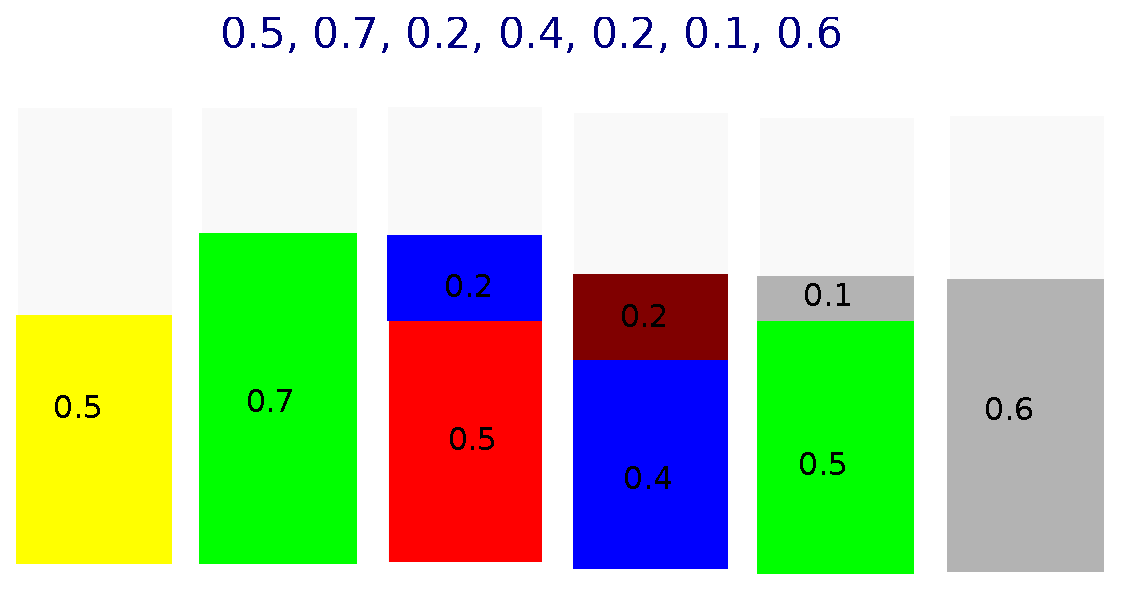
\includegraphics[width=100mm]{maxresdefault.eps}% bin-packing
	\caption{Primjer binarnog pakovanja.}
    \label{fig:bin-packing}
\end{figure}

Navedimo   \emph{prvi odgovarajući} (eng. {first-fit}) pohlepni algoritam, koji se sastoji od sljedećih koraka.
\begin{itemize}
	\item Raspoređujemo proizvode u onom redu u kojem su poredani za pakovanje, tj. $a_i$ se pakuje prije $a_j$ akko $i < j$;
	\item Stavljamo sljedeći proizvod u pakovanje sa najmanjim indeksom, u kojem je ostalo dovoljno prostora za taj proizvod.
	 \item Ako proizvod ne može da se ubaci ni u jedno otvoreno pakovanje, uzimamo novo pakovanje i tu smještamo taj proizvod.
\end{itemize}


Lako se vidi da je ovaj algoritam polinimijalne složenosti i da kao rezultat vraća dopustivo rješenje.  Neka je $C^*$ optimalan broj pakovanja koji se treba otvoriti da bi se spakovalo svih $n$ stavki. Pretpostavimo da algoritam vraća rješenje $C$ (pakovanja). Sigurno vrijedi da je barem u $C-1$ pakovanja  iskorišteno više od polovine prostora. Ako to ne bi bio slučaj, onda bi postojala dva pakovanja u kojima je najviše pola prostora iskorišteno. U tom slučaju, stavke u oba pakovanja bi mogle da idu u jedno od njih, dok bi se drugo oslobodilo. Prema tome, imamo
$$C^* \geq \sum_{i=1}^n a_i > \frac{C-1}{2}\ \Rightarrow\  2 \cdot C^* > C-1 \Rightarrow 2 \cdot C^* \geq C,$$
pa slijedi da je  algoritam  prvi-odgovarajući 2--aproksimacioni. 

Pomenimo sada i tzv. \emph{najbolji-odgovarajući} (eng. best-fit) algoritam, koji radi po sljedećem principu. Sljedeći proizvod se stavlja u ono pakovanje u kojem  ostaje najmanji prazan prostor, u odnosu na sva ostala otvorena pakovanja. Ako takvo pakovanje ne postoji, otvara se novo pakovanje. 
Ovaj algoritam je takođe 2--aproksimacioni. 

Interesantno je napomenuti da za problem binarnog pakovanja ne postoji aproksimativni algoritam čiji je faktor $c <\frac{3}{2}$ (osim ako je $P=NP$). 

 \subsection{Aproksimativni algoritmi za problem pokrivanja skupa}
\textit{Problem pokrivnja skupova} (eng. set cover problem) predstavlja uopštenje problema pokrivanja čvorova, i definisan je na sljedeći način.
\begin{definition}
    Neka je dat skup elemenata $X$ te familija podskupova $\mathcal{F}$ skupa $X$ takva da je za svaki $f\in \mathcal{F}$, $|f \cap X| \geq 1$ i $\bigcup_{f \in \mathcal{F}} f = X$. 
	    Potrebno je naći pokrivač $C \subseteq \mathcal{F}$ minimalne kardinalnosti takav da je 
	    $$ \bigcup_{f \in C} f = X.$$
\end{definition}


Motivacija za razmatranje ovog problema se može pronaći i u svakodnevnom životu. Npr. pretpostavimo da imamo skup sposobnosti (kompetencija), te skup ljudi koji posjeduju pojedine kompetencije. Potrebno je formirati komisiju sa što manjim brojem osoba, ali tako da se za svaku kompetenciju može naći osoba iz komisije sa tom kompetencijom.
 

 U nastavku ćemo objasniti pohlepni algoritam koji nema konstantan aproksimacioni faktor, već logaritamski zavisi od veličine ulaza. To znači da, kako veličina ulaza raste, kvalitet rješenja algoritma opada relativno u odnosu na kvalitet optimalnog rješenja. Ipak,  ovaj aproksimacioni algoritam  daje dobre rezultate u praktičnim primjenama, pošto logaritamska funkcija sporo raste.

\begin{figure}
	\centering
	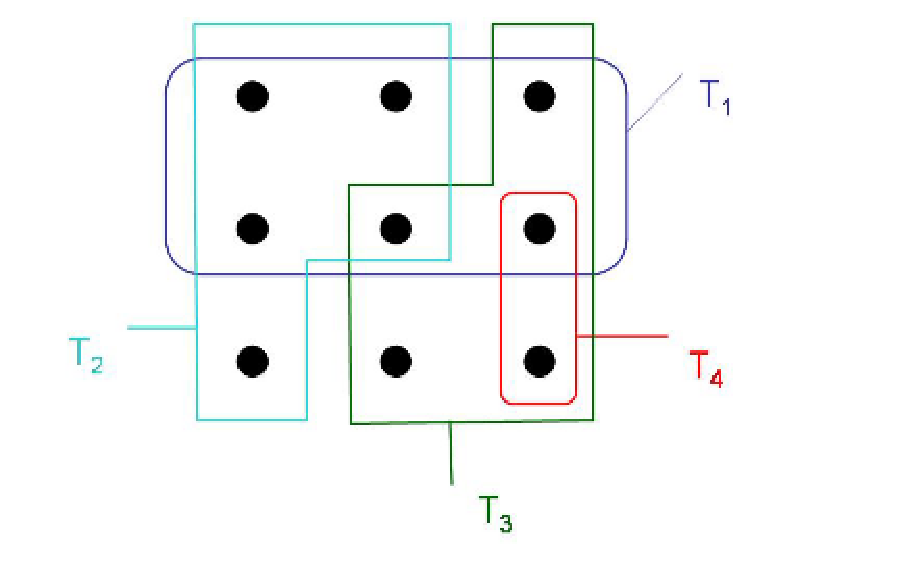
\includegraphics[width=120mm, height=80mm]{set-cover-1.eps}
	\caption{Primjer pokrivanja skupa ($\mathcal{F}=\{T_1,T_2,...,T_4\}$, optimalno rješenje je skup $\mathcal{C}=\{T_2, T_3\}$}
	 \label{fig:set-cover-1}
\end{figure}
 

 Pohlepni metod za problem pokrivanja skupa je prikazan Algoritmom~\ref{alg:set-cover-gridi}.  %objasnjenje algoritma.
Skup $U$ predstavlja skup preostalih nepokrivenih elemenata, dok skup $\mathcal{C}$ predstavlja pokrivač koji se konstruiše kroz iteracije algoritma. Incijalno, $U = X$, te pokrivač $C = \emptyset$.
U svakom koraku, algoritam nastoji da proširi pokrivač $\mathcal{C}$ na račun smanjenja skupa $U$. Kandidata za proširivanje pokrivača biramo na osnovu pohlepne funkcije date u liniji 6. U osnovi, biramo onaj  podskup $f \in \mathcal{F}$ koji ima maksimalan presjek sa trenutnim skupom $U$. Dati skup potom ubacujemo u rješenje $C$, te izbacujemo elemente iz $U$ koji se nalaze u skupu $f$. Algoritam se izvršava dok god ne pokrijemo sve elemente iz $U$, tj. dok god $U \neq \emptyset$.

Algoritam se izvodi u $O(|\mathcal{F}| \cdot |X|)$ vremenu, što znači da je polinomijalne složenosti. Takođe, jasno je da je rješenje koje se vraća dopustivo, uz pretpostavku da instanca generiše dopustiv prostor, što je lako provjeriti prije pokretanja algoritma. 

O aproksimativnom faktoru ovog pohlepnog algoritma nam govori naredna teorema, koju navodimo bez dokaza. %%Prije toga, označimo $d$-ti harmonijski broj $=H_d = \sum_{i=1}^d 1/i$ sa $H(d)$.

%Vrijedi sljedeća teorema.

%pseudokod algoritma 
\begin{algorithm}[!t] 
	\begin{algorithmic}[1]
		\STATE \textbf{Ulaz}: $X$ i familija podskupova $\mathcal{F}$ od $X$
		\STATE \textbf{Izlaz}: $C$ -- pokrivač skupa $X$
		\STATE $U \gets X$
		\STATE $C \gets \emptyset$
		\WHILE{$U \neq \emptyset$}
		\STATE $f \gets \mbox{argmax}_{f \in \mathcal{F} } |f \cap U | $
		\STATE $U \gets U \setminus f$
		\STATE $C \gets C \cup \{f\}$
		\ENDWHILE
	\end{algorithmic}
	\caption{GREEDY-SET-COVER metod za problem pokrivanja skupa.}
    \label{alg:set-cover-gridi}
\end{algorithm}

\begin{thm}
	  \mbox{GREEDY-SET-COVER} algoritam ima aproksimativni faktor 
	$$ H(\max\{|f| \mid f \in \mathcal{F}\}),$$
	gdje je $H(n) =\sum_{i=1}^n \frac{1}{i}$. 
\end{thm}

\begin{comment}
\fixme{Marko, ovaj dokaz je prilicno konfuzan. Ja bih ga izbacio. Ako ipak smatras da treba da ostane, onda predlazem da se ipak prvo pokaze da vazi (9.2), pa da se onda zakljucuje (9.3). Ovako je prilicno nejasno sta se dokazuje preko cega. Ako se dogovorimo da ostane, mozemo zajedno pokusati da malo uredimo dokaz. Ako se izbacuje, onda ni za tim nema potrebe.}

\begin{proof}
	  Označimo sa $f_i$, $i$-ti podskup koji je izabran od strane algoritma. Algoritam dodjeljuje cijenu $1$ kad se $f_i$ doda u $\mathcal{C}$. 
	  Cijenu izbora $f_i$ distribuiramo podjednakom vjerovatnoćom na sve elemente koji su po prvi put pokriveni sa $f_i$. Posmatrajmo primjer dat na Slici~\ref{fig:set-cover-1}. U prvoj iteraciji pohlepnog algoritma, 
	  6 elemenata je pokriveno sa $T_1$. Prema tome, cijena svakog od ovih elemenata je $c_x = \frac{1}{|T_1\setminus \emptyset|}= \frac{1}{6}$. Dalje, u drugoj iteraciji algoritam odabire skup $T_3$, koji pokriva 2 nova elementa. Njihova cijena je $c_x=\frac{1}{|T_3 \setminus T_1|} = \frac{1}{2}$. U iteraciji broj 3, odabere se skup $T_2$, te se pokriva jedan novi element. Njegova cijena je jednaka $c_x = \frac{1}{T_2 \setminus ( T_1 \cup T_3)}$. 
	 
	 Neka $ c_x$ označava cijenu za pokrivanje elementa $x\in X$.  Svakom elementu se cijena dodijeli najviše jednom, odnosno, pri prvom pokrivanju. Ako se $x$ pokriva prvi put sa $f_i$, tada imamo
	 $$c_x = \frac{1}{f_i \setminus (f_1 \cup ...\cup f_{i-1})}.$$
	 
	 Algoritam generiše rješenje $\mathcal{C}$, koje je cijene $|\mathcal{C}|$ i ova cijena se raspoređuje elemenatima iz $X$. Kako optimalni pokrivač $C^*$ takođe pokriva skup $X$, dobijamo
	 \begin{align}\label{eq:f1x}
	 	|C| = \sum_{x \in X} c_x \leq \sum_{f \in C^*}\sum_{x \in f} c_x.
	 \end{align}
	  Pokažimo sljedeću ključnu nejednakost. Za svaku $f \in \mathcal{F}$, vrijedi  
	 \begin{equation}\label{eq:f2x}
	 	\sum_{x \in f} c_x \leq H(|f|).
	 \end{equation}
	 
	 Iz formula~(\ref{eq:f1x}) i (\ref{eq:f2x}) se dobija da je 
	 \begin{equation}
	 	|C| \leq \sum_{f \in C^*}\sum_{x \in f} c_x \leq \sum_{f \in C^*} H(|f|),
	 \end{equation}
	 odakle slijedi tvrdnja o vrijednosti aproksimacionog faktora algoritma.
	 Ostaje nam još da pokažemo formulu~(\ref{eq:f2x}). 
	 
	 Neka je $f\in \mathcal{F}$ tako da za $i=1,\ldots,|C|$
	 $$u_i(f) = |f \setminus (f_1 \cup \cdots \cup f_{i} )|$$
	 
	 označava ostale elemente u $f \in \mathcal{F}$ koji su još uvijek nepokriveni nakon što je algoritam dodao skupove $f_1,\ldots, f_i$ u pokrivač $C$, posmatrano do $i$-te iteracije. Definišimo $u_0(f)=|f|$ za broj elemenata skupa $f$ koji je inicijalno nepokriven. 
	 Označimo sa $k$ prvi indeks tako da je $u_k(f)=0$  -- što znači da su svi elementi skupa $f$ u $k$-toj iteraciji
	 pokriveni prvi put nekim skupovima %$S_1,\ldots,S_i$
	 koji su odabranu u ranijim koracima algoritma. Primijetimo da vrijedi
	 $$ u_o(f) \geq u_1(f) \geq \ldots \geq u_{k-1}(f) \geq u_k(f).$$
	 Prema tome, $u_{i-1}(f) - u_{i}(f)$ predstavlja broj elemenata u skupu $f$ koji su pokriveni 
	 po prvi put sa $f_i$ u $i$-toj iteraciji za $i=1,\ldots,k$. Dakle, vrijedi
	 \begin{align}\label{eq:q1}
	 	\sum_{x \in f} c_x = \sum_{i=1}^k( u_{i-1}(f) - u_{i}(f)) \cdot \frac{1}{ f \setminus ( f_1 \cup \cdots \cup f_{i-1})},
	 \end{align}
 
   \noindent što je jednako sumi brojeva elemenata skupa $f$ pokriven sa $f_i$ pomnožen sa cijenom koja je dodjeljena svakom elementu u $i$-toj iteraciji. Primijetimo da vrijedi:
 \begin{align}\label{eq:q2x}
 	|f_i \setminus (f_1 \cup \cdots \cup f_{i-1})| \geq | f   \setminus (f_1 \cup \cdots \cup f_{i-1}) | := u_{i-1},
 \end{align}
 jer je $f_i$ pohlepni izbor (njegovim izborom pokrićemo čitav (nepokriveni dio) skupa $f_i$) u $i$-toj iteraciji i svaki drugi izbor ne može pokriti više novih (nepokrivenih elemenata). 
 
 Prema tome, iz jednakosti~(\ref{eq:f1x}), te nejednakosti~(\ref{eq:f2x}), slijedi 
 \begin{align*}
 	\sum_{x \in f} c_x \leq \sum_{i=1}^k ( u_{i-1} - u_{i}) \cdot \frac{1}{u_{i-1}}
 \end{align*}
 
 Izraz sa desne strane nejednakosti se može ograničiti na sljedeći način:
   \begin{align*}
 	   \sum_{i=1}^k ( u_{i-1} - u_{i}) \cdot \frac{1}{u_{i-1}} &= \sum_{i=1}^k \sum_{j=u_i + 1}^{u_{i-1}} \frac{1}{u_{i-1}} \leq \sum_{i=1}^k \sum_{j=u_i + 1}^{u_{i-1}}\frac{1}{j} \\
 	   &= \sum_{i=1}^k \left( \sum_{j=1}^{u_{i-1}}\frac{1}{j} - \sum_{j=1}^{u_{i}}\frac{1}{j} \right) \\
 	   &= \sum_{i=1}^k (H(u_{i-1}) - H(u_i)) \\
    	&= H(u_0) - H(u_k) = H(u_0) = H(|f|),
 \end{align*}
 
 odakle slijedi tvrđenje. 
 
\end{proof}

\fxnote{ovaj tekst ispod predlazem da ostane i njega sam malo popravio.}
\end{comment}

Napomenimo da postoji i težinska verzija problema pokrivanja skupa. U ovoj verziji je svakom skupu iz $f \in\mathcal{F}$ dodijeljena težina $w_f$. Zadatak je pronaći pokrivač $C \subseteq \mathcal{F}$ skupa $X$ sa najmanjom ukupnom težinom. Ovaj problem se,  uz pomoć sličnog pohlepnog algoritma kao kod netežinske varijante, može aproksimirati do na faktor $H_d= \log d+O(1)$, gdje je $d= \max\{|f|:f \in \mathcal{F}\}$. U tom slučaju, pohlepni kriterijum je određen funkcijom 
\begin{align}
	g(f) = \frac{w_f}{|f \cap U|}, f \in \mathcal{F}\setminus C,
\end{align}
gdje je $w_f$ težina skupa $f$. U svakom koraku algoritma određuje se skup $f^* \in \mathcal{F}$ koji minimizuje vrijednost funkcije $g$, koji se zatim dodaje u trenutni (parcijalni) pokrivač $C$.

\begin{comment}
\subsection{Aproksimativni algoritam za problem najkraćeg nadstringa}

Na kraju odjeljka o aproksimativnim algoritmima, razmotrimo i problem najkraćeg nadstringa.
\begin{definition}
   Neka je dat skup stringova $S=\{s_1,...,s_n\}$. Kod problema najkraćeg nadstringa potrebno je odrediti string  $s$ minimalne dužine koji sve stringove iz $S$ sadrži kao svoje (ne obavezno neprekidne) podstrigove. 
  \end{definition}
Napomenimo da je i ovaj problem NP--težak. 
 Da bismo konstruisali aproksimativni algoritam za ovaj problem, koristićemo tehnike razvijene za rješavanje Problema pokrivanja skupa iz prethodne sekcije i pokazaćemo da postoji $2\cdot H_n$--aproksimacija za problem najkraćeg nadstringa. 

Bez gubljenja opštosti, mozemo pretpostaviti da niti jedan string $s_i$ nije podstring stringa $s_j, i\neq j$.

 Svakom stringu $\theta$ dodijelimo skup $set(\theta)$, pri čemu   $set(\theta)$ pokriva string $s\in S$ akko 
je $s$ podstring od $\theta$. Prema tome 
$$set(\theta) = \{ s \in S \mid s \mbox{  podstring od }\theta \}.$$



 Odatle bi pokrivač skupa bila familija takvih skupova $set(\theta)$, iz kojih se konstruiše nadstring skupa $S$ spajajući sve $\theta$ stringove u jedan string. U svakom slučaju familija  $\mathcal{F}$ se ne može definisanti kao skup skupova $set(\theta)$ jer bi u suprotnom $\mathcal{F}$ bio beskonačan. Sa druge strane, ne možemo ograničiti sve stringove $\theta$ samo na one iz $S$, jer bismo u suprotnom dobili rješenje koje je jednako spajanju svih stringova iz $S$, što je svakako  rješenje koje nije korisno. Za uspostavljanje balansa,  iz skupa $S=\{s_1,...,s_n\}$ uzmimo jedan par stringova $s_i$ i $s_j$. Pronađimo $k>0$,  tako da je posljednjih $k$ karaktera stringa $s_i$ jednako podnizu   prvih $k$ karaktera stringa $s_j$ (postoji poklapanje ta dva stringa). Označimo sa $\theta_{ijk}$ string koji se 
dobije preklapanjem stringova $s_i$ i $s_j$ na $k$ karaktera. Oznacimo sa $I$ skup strinova $\theta_{ijk}$  za validne izbore $i,j$ i $k$. Zatim definišemo $\mathcal{F}=\{set(\theta) \mid  \theta \in S \cup I\}$. Dodijeljena cijena svakog skupa $set(\theta)$ je jednaka $|\theta|$. Na osnovu prethodnog, dobijamo algoritam za rješavanje problema Najkraćeg nadstringa, prikazanog Algoritmom~\ref{alg:ss}. 

  \begin{algorithm}[!t] 
	\begin{algorithmic}[1]
		\STATE \textbf{Ulaz}: skup $S=\{s_1,...,s_n\}$
		\STATE \textbf{Izlaz}: aproksimacioni nadstring $s$
		\STATE Izračunati instancu $(X,\mathcal{F})$ problema najkraćeg nadstringa
		\STATE  $\mathcal{C}=\{set(\theta_1), set(\theta_2),...,set(\theta_p)\}\gets$ Primijeniti GREEDY-SET-COVER$(X,\mathcal{F})$
		\STATE  $s \gets \theta_1 \cdots \theta_p$
	\end{algorithmic}
	\caption{Pohlepna heuristika za Problem Najkraćeg Nadstringa.}
	\label{alg:ss}
\end{algorithm}

\emph{Analiza algoritma}. 
Ako je $\mathrm{OPT}_{ns}$ vrijednost optimalnog rješenja problema  nad instancom $(X,\mathcal{F})$ za problem  najkraćeg nadstringa, a $\mathrm{OPT}_{ss}$ dužina najkraćeg nadstringa, može se pokazati da vrijedi 
$$\mathrm{OPT}_{ns} \leq 2 \cdot \mathrm{OPT}_{ss},$$
odakle slijedi da Algoritam~\ref{alg:ss} daje $2H_n$--aproksimaciju. 
  
  
 \section{Problem Pokrivanja Skupa: aproksimacioni algoritmi} 
 
  
 
   
  
  \section{Problem Najkraceg Nadstringa}
   
  
  Ideja za algoritam je svesti problem na problem pokrivanja skupa tako da je neophodno pokriti sve stringove iz $S$ da bi se ispunio uslov problema. 
  
  Svakom stringu $\theta$ dodijelimo skup $set(\theta)$ tako da skup $set(\theta)$ pokriva string $s\in S$ akko 
  je $s$ podstring od $\theta$. Prema tome 
  $$set(\theta) = \{ s \in S \mid s \mbox{  podstring od }\theta \}.$$
  
  Odatle bi pokrivac skupa bila familija takvih skupova $set(\theta)$, iz kojih se konstruise superstring skupa $S$ spajajuci sve $\theta$ stringove u jedan string. U svakom slucaju familija  $\mathcal{F}$ se ne moze definisanti kao skup skupova $set(\theta)$ jer bi u suprotnom $\mathcal{F}$ bio beskonacan. Sa druge strane, ne mozemo ograniciti sve stringove $\theta$ samo na $S$, jer bi u suprotnom dobili rjesenje koje je jednako konkatenaciji svih stringova iz $S$, sto je svakako nekorisno rjesenje. Za uspostavljanje balansa, neka iz skupa $S=\{s_1,...,s_n\}$ uzmemo par stringova $s_i$ i $s_j$, nadjemo $k>0$  tako da je posljednjih $k$ karaktera 
  stringa $s_i$ jednaka prvih $k$ karakera stringa $s_j$ (poklapanje). Oznacimo sa $\theta_{ijk}$ string koji se 
  dobije preklapanjem stringova $s_i$ i $s_j$ na $k$ karaktera. Oznacimo sa $I$ skup strinova $\theta_{ijk}$ 
  za validne izbore $i,j$ i $k$. Zatim definisemo $\mathcal{F}=\{set(\theta) \mid  \theta \in S \cup I\}$. Dodijeljena cijena svakog skupa $set(\theta))$ je jednaka $|\theta|$. Na osnovu prethodnog, dobijamo algoritam za rjesavanje problema Najkraceg Nadstriga pseudokodom~\ref{alg:ss}. 
  
  \begin{algorithm}[!t] 
  	\caption{Gridi heuristika za Problem Najkraceg Nadstringa.}\label{alg:ss}
  	\begin{algorithmic}[1]
  		\STATE \textbf{Ulaz}: skup $S=\{s_1,...,s_n\}$
  		\STATE \textbf{Izlaz}: aproksimacioni nadstring $s$
  		\STATE Izracunati instancu $(X,\mathcal{F})$ problema najkraceg nadstringa
  		\STATE  $\mathcal{C}=\{set(\theta_1), set(\theta_2),...,set(\theta_p)\}\gets$ Primijeniti GREEDY-SET-COVER$(X,\mathcal{F})$
  		\STATE  $s \gets \theta_1 \cdots \theta_p$
  	\end{algorithmic}
  \end{algorithm}
  
  Analiza algoritma. Ako je $\mathrm{OPT}_{ns}$ vrijednost optimalno rjesenje problema  nad instancom $(X,\mathcal{F})$ problema Najkraceg Nadstringa, a $\mathrm{OPT}_{ss}$ duzina najkraceg nadstringa, moze se pokazati da vrijedi 
  $$\mathrm{OPT}_{ns} \leq 2 \cdot \mathrm{OPT}_{ss}.$$
  
  Iz prethodnog bi slijedilo da Algoritam~\ref{alg:ss} daje $2H_n$--faktor aproksimaciju. 
  
 \end{comment} 
  
\section{Heurističke metode}
 U prethodnom odjeljku smo vidjeli da za aproksimativne algoritme vrijedi važna osobina da se rješavanjem problema ne garantuje pronalazak optimalnog rješenja, ali postoji garancija da se rješenje nalazi unutar nekog faktora kvaliteta ($c$), u odnosu na optimalno rješenje.  
 Drugim riječima, za rješenja dobijena aproksimativnim algoritmima se zna koliko njihov kvalitet maksimalno može da odstupa od kvaliteta optimalnog rješenja. 
 %, a to odstupanje je određeno faktorom kvaliteta.
 
 Posebna vrsta neegzaktnih metoda, odnosno metoda koje ne daju i/ili ne garantuju pronalazak optimalnog rješenja pri završetku su tzv. heurističke metode. 
 
 Za razliku od aproksimativnih algoritama, kod heurističkih metoda, u opštem slučaju, ne propisuje se faktor kvaliteta rješenja, već je primarni cilj razviti i primijeniti tehniku pomoću koje se u razumnom vremenu može doći do dovoljno dobrog (zadovoljavajućeg) rješenja. Heurističke metode mogu biti izvedene iz teorijskih razmatranja, ali i iz eksperimentalnih rezultata. Npr. u praksi je čest slučaj da se heurističke metode razvijaju na osnovu rješavanja problema manjih dimenzija ili uopštavanjem tehnika uspješno primijenjenih na uzorcima. 
 
 
 Snaga heurističkih algoritama leži u smanjenju prostora pretraživanja i usmjeravanju procesa pretraživanja u one regione koji sadrže bolja rješenja, čime se značajno ubrzava proces pronalaženja rješenja. Naravno, ne postoji univerzalna strategija koja garantuje uspjeh heurističkog algoritma, tj. ne postoji garancija da će heuristički algoritam uvijek pronaći dovoljno dobro rješenje u razumnom vremenu. Ipak, višedecenijski razvoj i upotreba različitih heurističkih algoritama ukazuju na činjenicu da ove metode zauzimaju veoma važno mjesto u oblasti kombinatorne optimizacije, a njihova uspješna primjena u širokom spektru različitih problema dokazuje njihovu stvarnu upotrebnu vrijednost.
 
 
 Svaka heuristička metoda mora da zadovolji dva pravila: da je rešenje ,,dovoljno
 dobro'' i da se algoritam pokrenut na ulazni problem izvršava u realnom, polinomijalnom vremenu. Treba napomenuti da se pod  ,,dovoljno
 dobrim'' rješenjem podrazumijevaju različite procjene, koje mogu biti subjektivne (npr. zasnovane na ličnoj ili profesionalnoj procjeni stručnjaka koji razvija ili koristi metodu), objektivne (npr.  rješenje je dobro ako od optimalnog rješenja odstupa u dozvoljenim granicama) ili zavisne od drugih uslova (npr. traži se rješenje problema takvo da je ono ekonomski prihvatljivo, bez obzira na to da li je blizu optimalnog rješenja ili ne). 
 Za neke metode, kvalitet dobijenog rješenja je moguće utvrditi samo eksperimentalno, npr. poređenjem sa rješenjima dobijenim uz pomoć drugih metoda. Nekada je cilj heurističke metode samo da se pronađe jedno dopustivo rješenje, dok se kvalitet samog rješenja ne razmatra.
 
 Važna osobina dobro konstruisanih heurističkih metoda je mogućnost prevazilaženja lokalnog ekstrema (što nije slučaj sa pohlepnim algoritmima), u cilju dostizanja globalnog optimalnog rješenja. 
 
 Takođe, heurističke metode se često uspešno mogu integrisati i u egzaktne metode, čime se kombinuje brzina dobijanja rješenja i potvrđivanje optimalnosti.
 
 \section{Metaheurističke metode}
 
 Široku klasu heurističkih metoda čine tzv. ,,univerzalne'' heurističke metode, koje se, uz blage modifikacije i prilagođavanje, mogu koristiti za rješavanje više različitih problema. Takve metode nazivamo \emph{metaheurističkim} metodama, ili metaheuristikama.  
 
 Metaheuristika se formalno definiše kao iterativni proces koji koristi približne metode, kombinujući na inteligentan način različite koncepte za pretraživanje prostora rješenja, da bi se u razumnom vremenu, ,,dohvatilo'' rješenje što bliže optimalnom.
 
 Sa praktičnog aspekta, cilj metaheuristika je pretraživanje skupa dopustivih rješenja, pri čemu je, ponekad, dozvoljeno i proširenje tog skupa elementima koji nisu dopustivi, prelazak u rješenja slabijeg kvali\-teta kako bi se izbjegli lokalni optimumi koji nisu i globalni, kombinovanje sa drugim heuristikama, itd.
 
 \subsection{Klasifikacija metaheuristika}
 S obzirom na veliki broj raznih metaheuristika koje su razvijene u posljednje vrijeme, prirodno je očekivati da se za  njihov razvoj koriste vrlo različiti pristupi, počev od polazne motivacije, preko strategije pretraživanja, različitih namjena i klasa problema na kojima se primjenjuju.
 U savremenoj literaturi, sreće se nekoliko kriterijuma za klasifikaciju metaheuristika.
 
 Klasifikacija metaheuristika prema polaznoj motivaciji identifikuje tzv. metaheuristike zasnovane na simulaciji prirodnih pojava (eng. \emph{nature inspired metaheuristics}), kao što su na primjer genetski algoritmi, mravlje ili pčelinje kolonije ili elektromagnetizam. Nasuprot njima, veliki broj metaheuristika nije motivisan prirodnim procesima, kao npr. tabu pretraživanje, iterativna lokalna pretraga itd.
 
 Prema broju tačaka kojima se raspolaže unutar jedne iteracije, metaheuristike se dijele na dvije klase: metaheuristike zasnovane na populaciji (eng. \emph{population based}) i metaheuristike koje rade sa jednom tačkom unutar jedne iteracije (eng. \emph{single point search}). U prvoj klasi, u datom trenutku algoritam raspolaže sa više tačaka -- različitih rješenja problema. Pretraživanje prostora je zasnovano na primjeni različitih operatora kombinovanja, pomjeranja, izmjena i odabira pojedinih tačaka, kako bi se u svakoj novoj iteraciji formirala nova populacija, sa potencijalno boljim rješenjima. Takve metaheuristike su: genetski algoritmi, mravlje kolonije, elektromagnetizam, jata ptica, itd.
 U metaheuristikama koje raspolažu jednom tačkom, primjenjuje se strategija zasnovana na praćenju trajektorije (eng. \emph{trajectory methods}), koja podrazumijeva da se kroz iteracije formira niz rješenja, od kojih je svako naredno (po pravilu, ali ne i obavezno) bolje od prethodnog. Ovi algoritmi najčešće, ali opet ne i obavezno, koriste i neke metode lokalnog pretraživanja, gdje se novo, potencijalno bolje rješenje bira unutar neke okoline trenutnog rješenja. Neke od metoda koje pripadaju ovoj klasi su metoda promjenljivih okolina, tabu pretraživanje, simulirano kaljenje, metoda promjenljivih okolina, itd.
 
 Prema tipu funkcije cilja, metaheuristike se mogu klasifikovati na one koje koriste statičku, te one koje koriste dinamičku funkciju cilja. Kako i sam termin ukazuje, dinamičke funkcije cilja se ažuriraju prema trenutnim zahtjevima u toku samog izvršenja metaheuristike. Suprotno njima, statičke funkcije se ne mijenjaju za vrijeme izvršenja metaheuristike. 
 
 Neke od najčešće korištenih metaheuristika su:
 \begin{itemize}
 	\item pohlepni algoritam sa prilagođenom slučajnom pretragom (eng. \emph{greedy randomized adaptive search procedure}) -- GRASP;
 	\item tabu pretraživanje (eng. \emph{tabu search}) -- TS;
 	\item genetski algoritam (eng. \emph{genetic algorithm}) -- GA;
 	\item metod promjenljivih okolina (eng. \emph{variable neighborhood search}) -- VNS;
 	\item simulirano kaljenje (eng. \emph{simulated annealing}) -- SA;
 	\item mravlje kolonije (eng. \emph{ant colony optimization}) -- ACO;
 	\item pčelinje kolonije (eng. \emph{artificial  bee colony}) -- ABC;
 	\item elektromagnetizam (eng. \emph{electromagnetism}) -- EM;
 	\item optimizacija rojem čestica (eng. \emph{particle swarm optimization}) -- PSO;
 	\item upravljano lokalno pretraživanje (eng. \emph{guided local search})  -- GLS.
 \end{itemize}
 
 U nastavku ovog poglavlja, detaljnije će biti objašnjena po jedna metaheuristika iz grupe populacionih metoda (genetski algoritam) i iz grupe metoda koje u procesu pretrage raspolažu samo jednom tačkom (metoda promjenljivih okolina). Pored ove dvije metode, biće objašnjen i princip lokalnog pretraživanja. Čitaocu preporučujemo da se, koristeći se internet izvorima, manje ili više detaljno upozna i sa drugim metaheuristikama, koje su nabrojane u ovom odjeljku.
 
  
 \subsection{Metoda lokalne pretrage}\label{sec: local_search}
 
 Metoda lokalne pretrage je tehnika čija se strategija sastoji u izvođenju niza poboljšanja  rješenja, počevši od nekog unaprijed zadanog, radeći ,,male'' promjene u strukturi trenutno najboljeg rješenja. Uvedimo prvo koncept okolina i lokalnih rješenja kao baznih pojmova u metodologiji lokalne pretrage. Za dato rješenje $x$, definišimo skup (ne obavezno dopustivih) rješenja koja su ,,blizu'' $x$ u odnosu na neku mjeru. Formalno, okolina predstavlja preslikavanje  $\mathcal{N}$ gdje svakom (dopustivom) rješenju pridružujemo skup rješenja, koje zovemo okolina od $x$.  Funkcija okoline se takođe može definisati preko operatora  $\Delta$, koji predstavlja kolekciju   funkcija $\Delta:\Phi \mapsto \Phi$,  gdje je $\Phi$ prostor pretrage (rješenja) razmatrane instance problema:
 $$ x' \in \mathcal{N}(x) \Longleftrightarrow \exists \delta \in \Delta,\delta(x)=x'.$$
 
 Prirodan izbor u mnogim aplikacijama je $k$-izmjenjena (eng. \emph{k-exchange}) okolina: $x$ i $x^{'}$ pripadaju istoj okolini akko se razlikuju na tačno $k$ komponenti rješenja. Npr. za TSP problem, 2-{izmijenjena} okolina je prirodan izbor gdje su komponente rješenja grane datog grafa.  
 
 
 Rješenje $x$ je \emph{lokalni optimum} u odnosu na okolinu $\mathcal{N}$ akko
 $f(x) \leq f(x')$ ($f(x) \geq f(x')$), za sve $x' \in \mathcal{N}(x)$, ako minimizujemo (maksimizujemo) ciljnu funkciju $f$.  \emph{Globalni optimum} je rješenje koje je lokalni optimum u odnosu na bilo koju okolinu.  Iako je to većini čitalaca jasno, nije zgoreg  još jednom pomenuti da nije svaki lokalni optimum ujedno i globalni. 
 
 \begin{algorithm}[!t] 
 	\caption{Lokalna pretraga (maksimizacija)}\label{alg:ls}
 	\begin{algorithmic}[1]
 		\STATE \textbf{Ulaz:} instanca problema, okolina $\mathcal{N}$
 		\WHILE{$ \left\{ x' \ni \mathcal{N}(x) \mid f(x') > f(x)\right\} \neq \emptyset$}
 		\STATE $ x \gets  \text{ izaberi } x' \in \mathcal{N}(x) $ ako vrijedi  $f(x') > f(x)$ 
 		\ENDWHILE
 	\end{algorithmic}
 \end{algorithm}
 
 Pseudokod lokalne pretrage je dat u Algoritmu~\ref{alg:ls}. Ulaz u algoritam je instanca problema i jedna unaprijed definisana okolina $\mathcal{N}$. U svakoj iteraciji, lokalna pretraga poboljšava trenutno (najbolje) rješenje ako    rješenje u okolini  $\mathcal{N}(x)$ ima bolju vrijednost ciljne funkcije. Algoritam se prekida ako je trenutno rješenje lokalno najbolje u odnosu na definisanu okolinu.
 Postoje dvije strategije za izbor rješenja koje će zamijeniti trenutno najbolje rješenje, pod pretpostavkom da postoji više od jednog rješenja sa boljom vrijednošću ciljne funkcije u posmatranoj okolini. Te strategije su:
 \begin{itemize}
 	\item \emph{prvo poboljšanje} (eng. \emph{the first improvement strategy}) -- ova strategija prihvata prvo nađeno rješenje $x'$ u okolini $\mathcal{N}(x)$ sa boljom vrijednošću ciljne funkcije od $x$. Pretraga se  pomjera u tačku  $x = x'$, odakle se pokreće nova iteracija lokalne pretrage. Lokalna pretraga se zaustavlja kada nema više poboljšanja.
 	\item \emph{najbolje poboljšanje} (eng. \emph{the best improvement strategy}) --   ova strategija provjerava sva rješenja iz okoline $\mathcal{N}(x)$ i za novo najbolje rješenje bira ono koje je lokalno najbolje u toj okolini. Nalazak  najboljeg rješenja zahtijeva enumeraciju svih rješenja iz okoline. Stoga, upotreba ove strategije, u opštem slučaju, zahtijeva više procesorskog vremena, tako da ona nije uvijek primjenjiva. U ovom slučaju, lokalna pretraga se završava kada nema više poboljšanja. %Ipak, u praksi se pokazalo da strategija \emph{najboljeg poboljšanja} često vodi ka lokalnom optimumu problema u svega nekoliko iteracija lokalne pretrage. 
 \end{itemize}
 Okolina kod koje se formira direktnom razmjenom vrijednosti dvije promjenljive u rješenju se često naziva i \emph{1-razmjena} (eng. \emph{swap}) okolina.
 \begin{primjer} U   problemu 0-1 ruksaka, za okolinu $\mathcal{N}$ bi mogli uzeti $1$-\emph{exchange} okolinu. Recimo, za $n=4$ i rješenje $x=1100$ imali  bismo $$\mathcal{N}(x)= \{ 0100, 1000, 1110, 1101 \}.$$ 
 \end{primjer}
 
 
 \subsection{Genetski algoritmi}\label{intro:ga}
 
 
 Genetski algoritmi spadaju u klasu populacionih i evolucijskih algoritama, čije je ponašanje inspirisano procesom evolucije koja se odvija u prirodi.
 Kao što je već rečeno, u osnovi se podrazumijeva rad sa populacijom rješenja (jedinki), gdje svaka jedinka predstavlja potencijalno rješenje polaznog problema, dok je populacija  podskup ukupnog prostora pretraživanja. Populacija se u iterativnom postupku mijenja tako što se stare jedinke mijenjaju novim, potencijalno boljim jedinkama.
 
 Osnovni okvir za funkcionisanje genetskih algoritama je prezentovan još 1975. godine od strane Džona Holanda, u čuvenoj knjizi ,,Adaptation in natural and artificial system''.
 
 Svakoj jedinki se dodjeljuje brojna vrijednost, tzv. \textit{prilagođenost} (eng.   {fitness}), koja ocjenjuje kvalitet posmatrane jedinke. Cilj genetskog algoritma je da se, iz iteracije u iteraciju, pronalaze jedinke sa sve boljom prilagođenošću, pod čime se smatra i pojedinačno poboljšanje nekih jedinki, ali i prosječna prilagođenost kompletne populacije, što se postiže standardnim genetskim operatorima: \textit{selekcijom}, \textit{ukrštanjem} i \textit{mutacijom}.
 
 Populacija je centralna struktura kod genetskog algoritma i ona  obično broji od nekoliko, pa do nekoliko stotina jedinki (u rijetkim situacijama i do hiljadu). Svaka jedinka se predstavlja genetskim k\^odom, koji se zapisuje nad nekom konačnom, najčešće binarnom ili  cjelobrojnom azbukom. Segmenti genetskog k\^oda se nazivaju \emph{geni}. 
 
 
 Početna populacija se obično kreira na slučajan način, čime se omogućava kreiranje raznovrsnog genetskog materijala, korisnog za kasnije faze algoritma i raznovrsnost samih jedinki. U nekim slučajevima se za generisanje polaznih jedinki koristi i neka druga heuristika, čime se pretraga od početka usmjerava ka onim oblastima pretraživanja za koje se pretpostavlja da sadrže kvalitetnija rješenja.
 
 Tokom rada algoritma, na populaciju se primjenjuju genetski operatori selekcije, mutacije i ukrštanja. Pored ovih osnovnih operatora, na neke jedinke se mogu primijeniti i drugi operatori, čijom se primjenom teži ka poboljšanju rješenja (na primjer, na neke, ili sve jedinke se mogu primijeniti i tehnike lokalnog  pretraživanja).
 
 \emph{Operator selekcije} bira jedinke na koje se dalje primjenjuju genetski operatori ukrštanja i mutacije. Po pravilu, boljim jedinkama, odnosno jedinkama sa boljom prilagođenošću, se operatorom selekcije daje veća vjerovatnoća da će biti izabrane, dok  slabije jedinke selekcijom dobijaju manju šansu. Postoji veći broj tehnika selekcije, a najpoznatije su: jednostavna (ili rulet) selekcija, turnirska, eliminacijska selekcija i elitizam. Rulet selekcija diktira da je vjerovatnoća da će jedinka biti izabrana proporcionalna prilagođenosti. Kod turnirske selekcije se iterativno formiraju skupovi jedinki, od kojih samo ona sa najboljom prilagođenošću opstaje i ulazi u dalji proces kombinovanja sa drugim jedinkama. Eliminacijska selekcija je primarno zasnovana na izbacivanju loših jedinki, prije nego na odabiru boljih za narednu generaciju. Značajan broj savremenih implementacija genetskog algoritma uključuje i koncept \emph{elitizma}. Elitizam podrazumijeva da će nekoliko najboljih (elitnih) jedinki direktno preći u narednu generaciju.
 
 \emph{Ukrštanjem} se kombinuju geni jedinki. Rezultat ukrštanja jedinki su nove jedinke, koje potencijalno sadrže ,,dobre'' gene  roditelja od kojih su nastale. Ovim mehanizmom  i jedinke slabije prilagođenosti, ali koje sadrže dobre gene, dobijaju šansu da učestvuju u reprodukciji i prenesu ,,dobar'' genetski materijal na sljedeću generaciju. Najčešće korišteni operatori ukrštanja su tzv. jednopoziciono, odnosno dvopoziciono ukrštanje, kod kojih se određuje jedna, odnosno dvije pozicije između kojih se odvija razmjena genetskih k\^odova roditelja, respektivno.
 
 \emph{Mutacijom} se vrši slučajna promjena određenog gena (sa nekom malom vjerovatnoćom da će se mutacija desiti), čime se postiže mogućnost vraćanja dobrog genetskog materijala, ukoliko je on izgubljen primjenom operatora selekcije. Time se proces pretrage  ,,izvlači'' iz preuranjene konvergencije i usmjerava ka onim oblastima pretraživanja koje sadrže potencijalno bolje jedinke.
 
 
 Nakon primjene genetskih operatora, formira se naredna generacija. Populacija se tako sastoji od potomaka i nekih starijih jedinki koje su preživjele, s obzirom na njihov kvalitet (elitne jedinke). Produkcija novih generacija se nastavlja sve dok ne budu ispunjeni uslovi za završetak algoritma. Najčešći kriterijumi za završetak algoritma su dostignuto maksimalno vrijeme izvršenja, dostignut  maksimalan ukupan broj iteracija, ili dostignut maksimalan broj iteracija bez poboljšanja najboljeg rješenja.
 
 Jedna od mogućih varijanti genetskog algoritma je prikazana Algoritmom \ref{alg:gascheme}.
 
 %$N_{pop}$ označava ukupan broj jedinki u populaciji.  $N_{elite}$ je broj elitnih jedinki, dok su promjenljivima  $p_i$ i $obj_{i}$ predstavljene odgovarajuća jedinka sa njenom vrijednošću funkcije cilja.
 %\begin{figure}[htp]
 %	\centering
 %	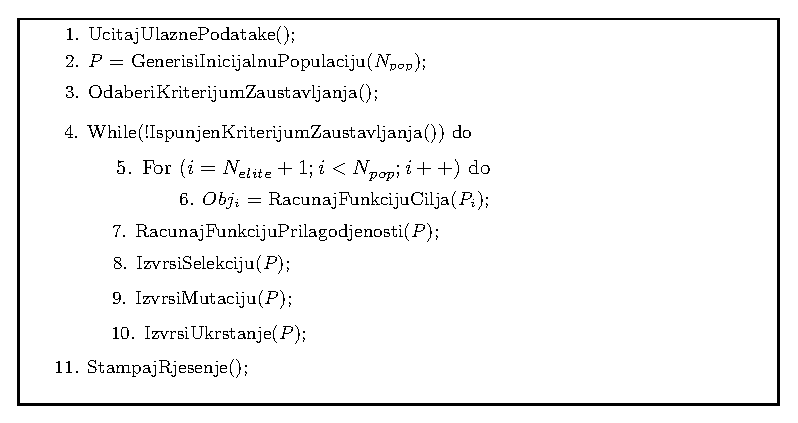
\includegraphics[width= 0.8\textwidth]{gasrp2.eps} \caption {Osnovna šema GA algoritma}\label{fig:gascheme}
 %\end{figure}
 
 \begin{algorithm}[!htb]
 	\begin{algorithmic}[1]
 		\STATE  $ P \gets GenerisiInicijalnuPopulaciju()$
 		\WHILE{!$IspunjenKriterijZaustavljanja()$}
 			\STATE $RacunajFunkcijuPrilagodjenosti(P)$
 			\STATE $P' \gets PrebaciElitneJedinke(P)$
 			\STATE $R \gets IzvrsiSelekcijuRoditelja(P)$
 			\STATE $P'' \gets IzvrsiUkrstanjeIMutaciju(R)$		  
 			\STATE $P\gets P' \cup P''$
 		\ENDWHILE
 	\end{algorithmic}
 	\caption{Osnovna šema GA.}
 	\label{alg:gascheme}
 \end{algorithm}
 
 Nakon što se generiše početna populacija $P$, pokreće se iterativni proces koji traje sve dok se ne ispuni kriterijum za zaustavljanje. Unutar iterativnog procesa, za svaku jedinku populacije $P$ se računa funkcija prilagođenosti. Nakon toga se, redom, formira skup $P'$, koji inicijalno sadrži elitne jedinke i skup $R$ koji je rezultat primjene operatora selekcije na populaciju $P$. Operatori ukrštanja i mutacije se primjenjuju na jedinke iz skupa $R$, a novodobijene jedinke se ubacuju u skup $P''$. Po izvršenju ovih operatora, populacija $P$ preuzima sve jedinke iz skupa $P'$ i $P''$ i iterativni proces se nastavlja.

\begin{primjer}\label{primjer:01ruksak} U ovom primjeru posmatrajmo 0-1 problem jednodimenzionalnog ruksaka. Ponovimo da nam je, kod ovog problema, na raspolaganju određen broj proizvoda, od kojih svaki proizvod ima svoju vrijednost i težinu. Ruksak je ograničenog maksimalnog kapaciteta (težine) $C$. Podsjetimo se i da se u 0-1 problemu ruksaka svaki proizvod ili ne uzima nikako ili se uzima kompletan. Cilj je, kao i u drugim problemima ruksaka, odabrati onaj skup proizvoda, tako da je njihova ukupna vrijednost maksimalna, a da se ne naruši kapacitet ruksaka.
\end{primjer}
Formalna matematička definicija 0-1 problema ruksaka će nam pomoći u konstrukciji genetskog algoritma, pa ćemo je ovdje navesti.

Neka je dato $n$ proizvoda, koji su opisani pomoću vektora $p$ i $w$. Neka $p_i$ i $w_i$ predstavljaju vrijednost i težinu $i$-tog proizvoda. Neka je $C$ maksimalan kapacitet ruksaka.

Neka je $f(\cdot)$ funkcija koja se maksimizuje i neka je $x$ binarni niz dužine $n$ koji predstavlja jedno rješenje problema: ako je $i$-ti proizvod uključen u rješenje, tada je $x_i = 1$, u protivnom, $x_i =0$. Ovaj problem se definiše sa ILP modelom
\begin{align*}
& \max\ \sum_{i=1}^{n}x_ip_i\\
&\mbox{t.d.}\\
&\sum_{i=1}^{n}x_iw_i\leqslant C\\
&x_i\in\{0,1\}, i = 1,2,\ldots,n
\end{align*}
Konstrukciju elemenata genetskog algoritma ćemo prikazati služeći se konkretnim primjerom. U Tabeli~\ref{tbl:01ruksak} su prikazani polazni podaci vezani za proizvode, a maksimalan kapacitet rukasaka je 22.

\begin{table}\begin{center}
	\begin{tabular}{lcc}\hline
		Proizvod&Cijena&Težina\\ \hline
		p1&5&7\\
		p2&8&8\\
		p3&3&4\\
		p4&2&10\\
		p5&7&4\\
		p6&9&6\\
		p7&4&4\\\hline
		\end{tabular}
	\end{center}\caption{Primjer instance za 0-1 problem ruksaka}\label{tbl:01ruksak}
\end{table} 

\emph{Kodiranje}. Genetski k\^od svake jedinke ćemo prikazati binarnim nizom dužine $n$ (u primjeru je $n=7$). Tako, na primjer, genetski k\^od 1100100 označava da su proizvodi pod rednim brojem 1, 2 i 5 uključeni u ruksak, dok ostali proizvodi nisu uključeni u ruksak. Vrijednost funkcije cilja za ovo rješenje je 5+8+7=20, dok je ukupna težina 7+8+4 = 19. 
Primijetimo da ovakav sistem kodiranja može da dovede do nedopustivih rješenja. Npr. genetski k\^od 0101010 označava da su proizvodi pod rednim brojem 2, 4 i 6 uključeni u rješenje, čija je ukupna težina 8+10+6 = 24, što je više od maksimalno dozvoljenog kapaciteta ruksaka.

Treba napomenuti da se u rješavanju velikog broja problema kombinatorne optimizacije pomoću genetskih algoritama, ali i drugih heurističkih metoda, često dozvoljava rad sa nedopustivim rješenjima. Razlog za to leži u činjenici da nisu sva nedopustiva rješenja ,,podjednako loša'', a nekada je lakše popraviti nedopustivo rješenje u dopustivo rješenje visokog kvaliteta, nego vršiti pretragu samo na prostoru dopustivih rješenja slabijeg kvaliteta.  Zbog toga se za prevazilaženje pojave nedopustivih rješenja najčešće koristi jedna od sljedeće dvije strategije: 
\begin{itemize}
	\item
	nedopustiva rješenja, po automatizmu, dobijaju minimimalnu vrijednost funkcije prilagođenosti, čime se omogućava da sam genetski algoritam odbaci takva rješenja u procesu selekcije. 
	
	\item uvodi se tzv. \textit{kaznena funkcija}  (eng. penalty function), kojom se ,,kažnjavaju'' nedopustiva rješenja (najčešće smanjenjem vrijednosti funkcije prilagođenosti), ali se ona ne izbacuju iz razmatranja, u nadi da perspektivnija nedopustiva rješenja mogu prerasti u kvalitetna dopustiva rješenja.
\end{itemize}

U našem primjeru, pojavu nedopustivih rješenja, dakle, možemo riješiti automatskom dodjelom minimalne vrijednosti funkcije prilagođenosti, ili ,,kažnjavanjem'' takvih rješenja smanjenjem vrijednosti funkcije prilagođenosti. Neke od strategije za ,,kažnjavanje'' nedopustivih jedinki bi mogle biti zasnovane na procjeni broja proizvoda koje treba zamijeniti (ili izbaciti) iz datog rješenja, a da rješenje postane dopustivo. Na taj način bi se ona nedopustiva rješenja, koja se teže mogu popraviti u dopustiva, više kažnjavala (i samim tim češće i odbacivala), dok bi se perspektivnija nedopustiva rješenja zadržavala u populaciji, u nadi da će, primjenom nekog od genetskih operatora, prerasti u kvalitetna dopustiva rješenja. Uopšte, vrijednost kaznene funkcije bi trebalo da bude malo veća od minimalne cijene potrebne da se odgovarajuće nedopustivo rješenje ,,popravi'' na dopustivo. Suprotno, ako bi vrijednost kaznene funkcije bila manja od cijene minimalne korekcije, nedopustiva rješenja se mogu javiti kao konačno rješenje, što naravno nije dopušteno. Sa druge strane, ako je vrijednost kaznene funkcije značajno veća od cijene minimalne popravke, nedopustiva rješenja su totalno diskriminisana i algoritam ih odmah odbacuje. 

\emph{Računanje funkcije prilagođenosti}. Za posmatrani problem, prirodna fukcija prilagođenosti bi se mogla definisati na način da ona bude jednaka ukupnom zbiru vrijednosti proizvoda uključenih u rješenje (pod uslovom da je to rješenje dopustivo), a da je vrijednost funkcije prilagođenosti  nedopustivih rješenja   jednaka nuli. 
Imajući u vidu prethodno razmatranje o nedopustivim rješenjima, funkcija prilagođenosti može biti definisana i drugačije, tj. mogla bi da sadrži i dio vezan za  ,,kažnjavanje'' nedopustivih rješenja, po nekom od predloženih (ili drugih) principa. Time bi nedopustiva rješenja bila uključena u pretragu.

\emph{Operator selekcije}. Ilustrujmo rad rulet selekcije na našem primjeru 0-1 problemu ruksaka. Naprije pretpostavimo da je funkcija prilagođenosti jednaka vrijednosti funkcije cilja. Dalje, posmatrajmo populaciju od 4 jedinke, prikazane u Tabeli~\ref{tab:rulet}.

Ukupna prilagođenost svih jedinki (zbir vrijednosti funkcija prilagođenosti svih jedinki) iznosi 72. Vjerovatnoće da će jedinke preživjeti za sljedeću generaciju jednake su redom: $\frac{18}{72},\ \frac{9}{72},\ \frac{17}{72}$ i $\frac{28}{72}$. 

Treba napomenuti da, iako se rulet selekcija na prvi pogled čini pogodnom za odabir jedinki koje preživljavaju u sljedećoj generaciju, ona ima i značajne nedostatke. Ovom selekcijom se jedinke sa slabom vrijednošću funkcije cilja često prerano odbacuju, iako možda sadrže potencijalno dobre gene, koji bi ukrštanjem sa drugim jedinkama mogli proizvesti još bolje potomke. Dalje, u kasnijim fazama algoritma, kada se javi više kvalitetnih jedinki koje imaju približno iste (ali ipak različite!) vrijednosti funkcije prilagođenosti, vjerovatnoće da će takve jedinke preživjeti su približno jednake, što dovodi do opasnosti da, nakon selekcije, najbolje jedinke i ne prežive u narednu generaciju. Stoga se u praksi značajno češće koristi turnirska selekcija, kojom se prevazilaze nedostaci rulet selekcije.


\begin{table}
	\centering
	\begin{tabular}{l|rrrrrrrrr}
		& \multicolumn{1}{l}{} & \multicolumn{1}{l}{} & \multicolumn{1}{l}{} & \multicolumn{1}{l}{} & \multicolumn{1}{l}{} & \multicolumn{1}{l}{} & \multicolumn{1}{l}{} & \multicolumn{1}{l}{prilagođenost} & \multicolumn{1}{l}{težine}  \\\hline
		Jedinka1 & 1                    & 0                    & 0                    & 0                    & 0                    & 1                    & 1                    & 18                         & 17                          \\
		Jedinka2 & 0                    & 0                    & 0                    & 0                    & 0                    & 1                    & 0                    & 9                          & 6                           \\
		Jedinka3 & 0                    & 1                    & 0                    & 1                    & 1                    & 0                    & 0                    & 17                         & 22                          \\
		Jedinka4 & 0                    & 1                    & 0                    & 0                    & 1                    & 1                    & 1                    & 28                         & 22      \\\hline                   
	\end{tabular}\caption{Primjer korišten za ilustraciju upotrebe rulet selekcije}
	\label{tab:rulet}
\end{table}

\emph{Operator ukrštanja}. Kao što je već pomenuto, osnovni operatori ukrštanja su tzv. jednopoziciono i dvopoziciono ukrštanje. Objasnimo primjerom jednopoziciono ukrštanje, koje bi moglo biti realizovano na sljedeći način
\begin{table}[H]
	\centering

\begin{tabular}{ccccc}
              &	Prije ukrštanja: &    &  Poslije ukrštanja:   \\
   Jednika 1: &	XXX $\mid$ XXXX  &    &   XXXYYYY             \\
   Jedinka 2:&	YYY $\mid$ YYYY  &    &   YYYXXXX             \\
\end{tabular}
	\caption{Primjer operatora ukrštanja: jednopoziciono ukrštanje.}
\end{table}
U ovom generičkom primjeru možemo vidjeti jednopoziciono ukrštanje u pozicijama $(3, 3).$  Specifičnije, pretpostavimo da imamo dva rješenja (jedinke) konstruisane u algoritamskom procesu: 1100100 i 0100011. Na osnovu jednopozicionog ukrštanja, one produkuju dva nova rješenja (dva potomka), tako što se lijevi dio genetskog k\^oda prvog roditelja spaja sa desnim dijelom genetskog k\^oda drugog roditelja i obrnuto, lijevi dio genetskog k\^oda drugog roditelja se spaja sa desnim dijelom prvog roditelja. 
Treba napomenuti da se primjenom ovakvog operatora ukrštanja takođe mogu dobiti potomci koji su nedopustivi, bez obzira na to da li su jedinke roditelja dopustive ili ne. Njihova dalja egzistencija u populaciji ponovo zavisi od načina konstruisanja funkcije prilagođenosti. 

Kod dvopozicionog ukrštanja postoje dvije pozicije u svakoj od jedinki na osnovu kojih se radi ukrštanje. Primjer ovakvog ukrštanja je data Tabelom~\ref{tbl:dvopozukr}
\begin{table}[H]
	\centering
	
	\begin{tabular}{ccccc}
		&	Prije ukrštanja: &    &  Poslije ukrštanja:                         \\\hline
		Jednika 1: &	XXX $\mid$ XXXX $\mid$ XX  &    &   XXXYYYYXX             \\
		Jedinka 2 :&	YYY $\mid$ YYYY $\mid$ YY  &    &   YYYXXXXYY             \\
	\end{tabular}
	\caption{Primjer operatora ukrštanja: dvopoziciono ukrštanje.}\label{tbl:dvopozukr}
\end{table}

U ovom primjeru ukrštanje je izvedeno u pozicijama $(3,7)$ prve jedinke i pozicijama $(3, 7)$ druge jedinke. Kao i kod jednopozicionog ukrštanja i ovdje je moguće da novonastale jedinke ne budu dopustive. 
\begin{table}[H]
	\centering
	
	\begin{tabular}{lc}
		Maska:      &   \verb|110001100|   \\\hline
		Jednika 1:  &	\verb|XXXXXXXXX|   \\ 
		Jedinka 2: &	\verb|YYYYYYYYY|   \\
		Poslije ukrštanja:  &       \\ \hline
		Nove jedinke:            &  \verb|XXYYYXXYY|    \\
		&  \verb|YYXXXYYXX|    \\
	\end{tabular}
	\caption{Primjer operatora ukrštanja: uniformno ukrštanje.}\label{tbl:uniukr}
\end{table}


Kod uniformnog ukrštanja, za svaki par jedinki koje se ukrštaju, prvo se generiše maska na slučajan način, tj. binarni niz dužine genetskog k\^oda jedinki. Ukoliko je na poziciji $i$ generisane maske vrijednost 1, onda prvi potomak za $i$-ti gen uzima vrijednosti prve jedinke, dok je $i$-ti gen drugog potomka vrijednost $i$-tog gena druge jedinke. Inače, vrijedi obrnuta situacija. Jedan primjer ovakvog ukrštanja je data Tabelom~\ref{tbl:uniukr}



\emph{Mutacija}. Kao što je pomenuto, mutacije podrazumijevaju male promjene u genetskom k\^odu, čija je osnovna namjena izlazak iz lokalnih podoptimalnih rješenja i omogućavanje dalje pretrage u cilju pronalaženja boljih rješenja. Najčešće se mutacija realizuje kao promjena vrijednosti jednog gena. U slučaju  0-1 problemu ruksaka, predstavljenog u Primjeru~\ref{primjer:01ruksak}, u zavisnosti od drugih elemenata algoritma, mogao bi se konstruisati veći broj različitih operatora mutacije: 
\begin{itemize}
	\item Mutacija 1: prelazak neke nule u jedinicu. Ova mutacija bi modifikovala trenutnu jedinku na način da se neki proizvod, koji nije bio u rješenju, uključi u rješenje. Time bi se povećala ukupna vrijednost ruksaka, ali postoji opasnost da jedinka postane nedopustiva.
	\item  Mutacija 2: prelazak neke jedinice u nulu. Ova mutacija bi modifikovala trenutnu jedinku na način da se neki proizvod, koji je bio u rješenju, isključi iz rješenja. Ovo bi dovelo do smanjenja ukupne vrijednosti ruksaka, ali bi, u slučaju rada sa nedopustivim jedinkama, postojala mogućnost da nedopustivo rješenje postane dopustivo (ili da se poboljša kvalitet nedopustivog rješenja).
	\item  Mutacija 3: dva gena različitih vrijednosti mijenjaju svoje vrijednosti. Preciznije, biraju se dva gena, od kojih jedan ima vrijednost 0, a drugi ima vrijednost 1, te prvi gen mijenja vrijednost na 1, a drugi na 0. Time se postiže da se, simultano, jedan proizvod, koji nije bio u rješenju, uključuje u rješenje, a drugi proizvod, koji je prije mutacije bio u rješenju, sada izbacuje iz rješenja. Kao i u prethodnim slučajevima, i ovdje je, na sličan način, potrebno razmatrati potencijalnu nedopustivost novonastale jedinke.
	\item Mutacija 4: zasnovana na tzv. uniformnoj mutaciji. Slično kao kod uniformnog ukrštanja, definiše se maska na osnovu koje se vrši mutacija određenih gena. Primjer ove mutacije dat je u Tabeli~\ref{tbl:unimut}. Nakon mutacije, kod jedinke će biti izmijenjeni geni koji su na pozicijama 1 i 5.
\end{itemize}



\begin{table}[H]
	\centering
	\begin{tabular}{lc}
		Maska:  &  1000100  \\
		Jedinka: & 1101000  \\ \hline
		Nakon mutacije &       \\
		               & 0101100      \\
	\end{tabular}	
	\caption{Primjer operatora mutacije (uniformno mutiranje)}\label{tbl:unimut}
\end{table}


Na kraju ovog odjeljka treba pomenuti da je višedecenijska primjena genetskih algoritama u rješavanju velikog broja problema kombinatorne optimizacije dovela je do pojave velikog broja različitih varijanti algoritma, koje se, između ostalog, razlikuju po operatorima koji se primjenjuju, načinu formiranja početne populacije, primjenama različitih strategija lokalnog pretraživanja, tehnike keširanja međurezultata, itd. 



  
\subsection{Metoda promjenljivih okolina}\label{intro:vns}
  
Metoda promjenljivih okolina (VNS) je metaheuristika uvedena od strane Nenada Mladenovića i Pjera Hansena 1997. godine.
Pretraga je zasnovana na sistematskoj promjeni okolina da bi se izbjegle situacije kada algoritam ,,upada'' u podoptimalna rješenja. Efikasnost VNS algoritma je zasnovana na razmatranju da u mnogim praktičnim optimizacionim problemima postoji povezanost između lokalnih optimuma. Stoga, metoda promjenljivih okolina i ne prati unaprijed zadatu putanju, već ,,skače'' na potencijalno bolja rješenja koja se nalaze u nekoj okolini trenutno najboljeg rješenja. Ovaj proces je poznat pod nazivom \textit{diversifikacija} (eng. \emph {diversification}). Sistem je dodatno ojačan procedurom lokalnog pretraživanja, kojom se  iz trenutnog rješenja prelazi u najkvalitetnije rješenje u nekoj njegovoj okolini. Ovaj proces je poznat pod nazivom \textit{intenzifikacija} (eng.  {intensification}).

Ponovimo da algoritam zasnovan na metodi promjenljivih okolina raspolaže jednom tačkom u jednoj iteraciji, a ne populacijom tačaka kao što je to slučaj sa genetskim algoritmom.

Tako, ideja da se pretraga usmjeri sa jednog na (moguće bolji) drugi lokalni optimum, koji je smješten u nekoj okolini polaznog lokalnog optimuma, predstavlja razuman  i, kao što je to slučaj u velikom broju raznih optimizacionih problema, opravdan pristup.
Da bi se postigli pomenuti efekti ,,iskakanja'' iz lokalnog (pod)optimuma, kao i detaljno pretraživanje nove okoline trenutnog najboljeg rješenja, metoda promjenljivih okolina se najčešće realizuje pomoću dvije važne procedure: procedure \textit{razmrdavanja} (eng.  {shaking}) i procedure \textit{lokalnog pretraživanja} (eng.  {local search}). Kao i što je to slučaj sa svim metaheurističkim metodama, dugogodišnja primjena metode promjenljivih okolina na rješavanje različitih problema dovela je do pojave velikog broja različitih varijanti, koje, pored osnovnih metoda razmrdavanja i lokalnog pretraživanja, uključuju i mnoge druge efektivne strategije.

Da bi se proširila pretraga,  VNS u potrazi za boljim lokalnim optimumom, obično koristi okoline rastuće kardinalnosti. Da bi se definisao skup okolina, pretpostavimo da je $x$ proizvoljno rješenje i $N_k$, za $k=k_{min},\ldots,k_{max}$, konačan skup  okolina. Tada se  $N_k(x)$ definiše kao skup rješenja u $k$-toj okolini tačke $x$. 
 Jedna od implementacija VNS metode, kojom se rješava problem maksimizacije, prikazana je Algoritmom~\ref{alg:vns}. 


 U svakom koraku algoritma, VNS započinje od nekog rješenja $x$ i cijelog broja $k$, $k_{min}\leqslant k\leqslant k_{max}$, koji označava trenutnu okolinu $N_k$. U proceduri razmrdavanja
 se na slučajan način bira rješenje  $x'$ iz okoline  $N_k(x)$. Zatim se na to rješenje primjenjuje procedura lokalnog pretraživanja. Najbolje rješenje koje se dobije u lokalnom pretraživanju se dalje poredi sa trenutno najboljim rješenjem i ukoliko je ono bolje od trenutno najboljeg rješenja, ono se proglašava novim najboljim rješenjem i algoritam nastavlja sa daljim izvršavanjem. Postoje različite strategije kada algoritam prelazi u narednu okolinu (u proceduri razmrdavanja), kao i kada se okoline ,,resetuju'', tj. kada se algoritam vraća na razmatranje najmanje okoline. 

 Najčešći kriterijumi za prekid   algoritma su: dostignuto maksimalno  vrijeme, dostignut maksimalan broj iteracija, maksimalni broj iteracija između dva poboljšanja najboljeg rješenja. %ili maksimalan broj ponavljanja najboljeg rješenja.

    \begin{algorithm}[!t] 
 	 \caption{VNS metaheuristika (maksimizacija)}\label{alg:vns}
  	\begin{algorithmic}[1]
		\STATE \textbf{Ulaz:} inicijalno rješenje $s$, okoline  $\mathcal{N}_{k_{\min}},\ldots, \mathcal{N}_{k_{\max}}$ 
		\STATE \textbf{Izlaz:} (poboljšano) rješenje $s$
		\STATE $k \gets  k_{\min}$
		\WHILE{!(\emph{IspunjenKriterijZaustavljanja()})}
		\STATE  $s' \gets$ izabrati random rješenje iz $\mathcal{N}_k(s)$ \hspace{0.3cm}//\,shaking faza 
		\STATE $s' \gets  LokalnaPretraga(s^{'})$
		\IF{$f(s') > f(s)$}
		\STATE $s \gets s'$
		\STATE $k \gets k_{min}$
		\ELSE 
		\STATE $k \gets k+1$ \hspace{0.3cm}//\, koristiti narednu (VNS) okolinu
		\IF{$k > k_{max}$}
		\STATE $k\gets k_{min}$
		\ENDIF
		\ENDIF
		\ENDWHILE
	 	\STATE \textbf{return} $s$
 	\end{algorithmic}
 \end{algorithm}


 \begin{primjer} Da bismo ilustrovali način funkcionisanja metode promjenljivih okolina, možemo posmatrati isti primjer kao i u slučaju genetskog algoritma: 0-1 problem ruksaka. 
 \end{primjer}

 \emph{Reprezentacija rješenja}. Kao i u slučaju genetskog algoritma, rješenje problema se može predstaviti binarnim nizom. Ako $i$-ti element niza ima vrijednost 1, to znači da je $i$-ti proizvod uključen u rješenje, a u suprotnom je izostavljen.

 \emph{Vrijednost funkcije cilja}. Slično kao u primjeru genetskog algoritma, vrijednost funkcije prilagođenosti se najlakše može definisati kao zbir vrijednosti proizvoda uključenih u rješenje. Eventualno, ako se u algoritmu dozvoljava rad sa nedopustivim rješenjima, funkcija prilagođenosti može da sadrži i dio za ,,kažnjavanje'' nedopustivih rješenja. Razmatranje o kažnjavanju nedopustivih rješenja je slično kao u slučaju genetskog algoritma.

 \emph{Razmrdavanje}. Može se primijeniti više različitih tehnika razmrdavanja, a u ovom primjeru ćemo objasniti jedan pristup. 
 U okviru procedure razmrdavanja, kreira se novo rješenje $x'$, ($x' \in N_k(x)$) zasno\-vano na trenutno najboljem rješenju  $x$.
 $k$-ta okolina se definiše na sljedeći način: Nekih $k$ proizvoda se bira na slučajan način. Svakom izabranom proizvodu mijenja se status: Ako je izabran proizvod koji je uključen u ruksak, on se izbacuje iz ruksaka i obrnuto. 

 Za pravilno funkcionisanje procedure razmrdavanja, potrebno je definisati kardinalnost najmanje i najveće okoline, koja zavisi od $k$. Obično se okolina najmanje kardinalnosti zasniva na malim vijednostima $k$, (na primjer $k_{min}=1$ ili $k_{min}=2$), dok se za maksimalnu vrijednost $k_{max}$  uzimaju vrijednosti 20, 30, ili čak i više, u zavisnosti od prirode i dimenzije problema.

  Praktično gledano, u našem primjeru u $k$-tom koraku izvršenja procedure razmrdavanja, naš algoritam bi generisao jedno novo rješenje (označimo ga sa $x'$), koje se od trenutno najboljeg rješenja razlikuje u tačno $k$ koordinata, odnosno u tačno $k$ proizvoda. Npr. u slučaju da je rješenje $x$ predstavljeno nizom 1100100 i ako je $k=3$, tada bi rješenje    $x'$ moglo da  (između ostalog) izgleda
 1000111. Odnosno, vidimo da se ova dva rješenja razlikuju na tačno tri indeksa (indeksima 2, 6 i 7).

 \emph{Lokalno pretraživanje}. 
 Za rješenje  $x'$ dobijeno u  proceduri razmrdavanja poziva se lokalno pretraživanje. Ova procedura podrazumijeva temeljno (ispcrpno) pretraživanje svih (ili skoro svih) rješenja, koja se blago razlikuju od rješenja  $x'$. Lokalno pretraživanje u ovom problemu bi moglo biti zasnovano na sličnim razmatranjima kao mutacije kod genetskog algoritma. Npr. jedno lokalno pretraživanje bi moglo da bude zasnovano na tzv. 1-\emph{zamjena} principu (eng. 1-swap, odnosno razmjeni vrijednosti parova koordinata. Preciznije, lokalno pretraživanje razmatra sva rješenja nastala od rješenja $x'$ na način da je jedan proizvod koji je bio uključen u ruksak sada izbačen, a neki drugi proizvod, koji prvobitno nije bio u ruksaku, sada jeste.

   Postoje različite strategije koliko dugo se izvršava lokalna pretraga. U opštem slučaju, potrebno je napraviti balans između utrošenog vremena pretraživanja i potrebe za lokalnim poboljšanjem rješenja. Stoga je generalno dobar pristup konstrukcija  procedura lokalnog pretraživanja koje se brzo izvršavaju, kako bi se, zbog velike brzine izvršavanja jedne iteracije lokalne pretrage, omogućilo što iscrpnije pretraživanje okoline datog rješenja u razumnom vremenu. Takođe, nekada se kombinuje više metoda lokalnog pretraživanja (ovo važi za većinu heurističkih metoda), koje, manje ili više temeljno, pretražuju okoline datog rješenja, u zavisnosti od brzine ili drugih parametara.



 \section{Zadaci}

 \begin{enumerate}
	\item Na šahovskoj tabli dimenzije 8x8 je postavljeno nekoliko topova, tako da se nikoja dva topa međusobno ne napadaju. Dodati na tu tablu još topova, tako da ih bude maksimalno 8, a da se i dalje nikoja dva topa ne napadaju.
	\item Istražiti na internetu problem vraćanja kusura pomoću minimalnog broja novčanica (kovanica). Koristi google pretragu \textit{change-making problem} ili \textit{coin change problem}. Napisati pohlepni algoritam koji rješava ovaj problem. Ispitati pod kojim uslovima pohlepni algoritam uvijek daje optimalno rješenje i pronaći kontraprimjer, kada pohlepni algoritam neće dati optimalno rješenje.

	
	\item Osmisliti pohlepni algoritam koji rješava problem trgovačkog putnika. Pronaći kontraprimjer kada taj algoritam ne pronalazi optimalno rješenje.
	
	\item Osmisliti pohlepni algoritam koji rješava problem određivanja maksimalnog nezavisnog skupa čvorova u grafu. Odredi neke klase grafova za koje taj pohlepni algoritam uvijek pronalazi optimalno rješenje. Pronaći kontraprimjer kada pohlepni algoritam ne pronalazi optimalno rješenje.
	
	\item Svaki razlomak se može napisati kao zbir razlomaka od kojih svaki ima jedinicu u brojiocu. Taj zapis su koristili još i stari Egipćani, po kojima se taj zapis i zove ,,egipatski razlomak''. 
	Napisati pohlepni algoritam koji proizvoljan razlomak zapisuje kao ,,egipatski razlomak'', odnosno kao zbir razlomaka koji imaju jedinicu u brojiocu.
	
	\item Zadat je skup $S$ koji se sastoji od $n$ brojeva. Koristeći pohlepni algoritam, podijeliti skup $S$ na dva podskupa, tako da se zbirovi elemenata u prvom i drugom podskupu što manje razlikuju.
	
	\item Neka je dato $N$ kajakaša koji su teški redom $1\leqslant w_1\leqslant w_2\leqslant \cdots \leqslant W_N$. Cilj je rasporediti kajakaše u što manje kajaka--dvosjeda. Maksimalna težina koju jedan kajak može da izdrži je $k$. Pretpostavka je da je za svako $i$, $w_i\leqslant k$. Napisati pohlepni algoritam koji rješava ovaj zadatak.
	
		%http://poincare.matf.bg.ac.rs/~ezivkovm/nastava/12_asp-pohlepni-algoritmi.pdf
	\item  Napisati pohlepni algoritam koji ispituje da li je jedna riječ podriječ druge riječi.
	
	\item Poznate su visine $n$ momaka i $n$ djevojaka. Napisati program koji
	određuje koliko se najviše plesnih parova može formirati tako da je momak uvijek
	viši od djevojke.
	\item Konstruisati primjer za 0-1 problem ruksaka, koji se ne može do optimalnosti riješiti pohlepnim algorimom prikazanom u Odjeljku~\ref{sec:frkacruksak}, koji se koristi za rješavanje frakcionog problema ruksaka.
	
	\item   U literaturi ili na internetu, pronaći primjere problema za koji postoji apsolutni apriksimativni algoritam (na primjer, bojenje planarnog grafa, eng. \emph{Planar graph coloring}), odnosno primjer problema za koji postoji relativni apriksimativni algoritam.
	
	\item Implementirati aproksimativne algoritme pomenute u Odjeljku~\ref{sec:binpack} i analizirati rješenja na različitim instancama problema.
	
	\item Implementirati genetski algoritam za rješavanje 0-1 problema ruksaka iz Primjera~\ref{primjer:01ruksak}.
	
	\item Problem postavljanja kraljica na šahovsku tablu podrazumijeva pozicioniranje kraljica tako da se nikoje dvije kraljice ne napadaju. Osmisliti genetski algoritam koji rješava ovaj problem.
		\item Bojenje grafa je procedura koja svakom čvoru grafa dodjeljuje jednu boju, poštujući pravilo da susjedni čvorovi nisu obojeni istom bojom. 
		\begin{enumerate}
			\item 	Napisati pohlepni algoritam pomoću kog se vrši bojenje grafa, tako da se iskoristi što je manje moguće boja.  Okarakterisati neku klasu grafova za koju  pohlepni algoritam uvijek daje optimalno rješenje. Konstruisati kontraprimjer kada pohlepni algoritam neće dati optimalno rješenje.
	\item Osmisliti genetski algoritam za rješavanje problema bojenja čvorova grafa.
	\item Osmisliti metodu promjenljivih okolina kojom se rješava ovaj problem
		\end{enumerate}
	
	\item Osmisliti genetski algoritam i metodu promjenljivih okolina kojima se rješava problem određivanja maksimalne klike u grafu.
	
		\item Osmisliti genetski algoritam i metodu promjenljivih okolina kojima se rješava problem određivanja maksimalnog nezavisnog skupa čvorova u grafu.
		\item %https://www.mpi-inf.mpg.de/fileadmin/inf/d1/teaching/winter15/ApproxAlg/ex01.pdf
		   Neka je dat ruksak čija je veličina jednaka $C$ i skup proizvoda $I = \{1,\ldots, n\}$, gdje proizvod $i$ ima svoju cijenu $c_i>0$ i veličinu $s_i>0$. Pokrivač ruksaka je skup proizvoda $I' \subseteq I$ tako da je $\sum_{i \in I'} s_i > C$.  Problem pokrivača ruksaka traži podskup proizvoda koji je pokrivač ruksaka sa minimalnom    cijenom.   Pretpostavimo da ne postoji proizvod čija je cijena veća od    cijene optimalnog rješenja. Konstruisati 2--aproksimativni algoritam za ovaj problem pod prethodnom pretpostavkom. 
		   \item Pokazali smo da postoji 2--aproksimativni algoritam za problem pokrivanja čvorova. Da li se može konstruisati instanca na kojoj neki od dva aproksimativna algoritma prikazana u Odjeljku~\ref{sec:aprokspokrivanjecvorova}, ne daje bolju aproksimaciju od faktora 2? 
 
		   \item %https://massivedatasets.files.wordpress.com/2011/04/approx1-exercisesf114.pdf
		   Neka je dat kompletan neusmjeren graf $G = (V, E)$ u kojem težine grana zadovoljavaju nejednakost trougla i neka je $k$ pozitivan prirodan broj. Problem metričkog $k$-klasterovanja (eng. Metric $k$-clustering)  se sastoji od particionisanja skupa $V$ na $k$ disjunktnih skupova $V_1, \ldots, V_k$, na način da se  minimizuje najveća cijena grane  između dva čvora u istom skupu, simbolički zapisano
		   $$ \min\max_{1 \leq i \leq k, u,v \in V_i} c(uv).$$
		   Konstruisati 2--aproksimativni algoritam za problem metričkog $k$--klasterovanja. 
		\item %https://www.ibr.cs.tu-bs.de/courses/ws1920/aa/exercises/exercise_03.pdf
		 Neka je dat   graf $G=(V,E)$. Naći particiju $V$ na $k$ skupova $V_1,\ldots, V_k$ tako da je broj grana koje su između dvije različite particije minimizovan. Konstruisati (pohlepni) algoritam koji je ($1-\frac{1}{k}$)--~aproksimativni. 
		 
 
		 \begin{comment}
		 \item U problemu bojenja grafa, u ulazu nam je dat neusmjeren graf $G = (V,E)$. Kažemo da je funkcija $f:V \mapsto \{1,\ldots, k\}$ $k$-bojenje akko ne postoje susjedni čvorovi grafa kojima je pridružen isti broj, tj. $f(u) \neq f(v)$, za $uv \in E$. Problem bojenja grafa traži za $k$-bojenje na grafu $G$, gdje je $k$ minimalan. Konstruisati pohlepni algoritam za koji je $k = \Delta + 1$, gdje je $\Delta$ maksimalni stepen čvora u $G$. 
		 \end{comment}
 
		 %\begin{comment}
		 \item %https://www.ibr.cs.tu-bs.de/courses/ws1920/aa/exercises/exercise_05.pdf
		 U ovom zadatku se rješava Problem obilaska segmenata (eng. \emph{Segment tour problem}). Neka je dat skup segmenata $S = \{s_0 = (p_0, p_1), s_1 =(p_2, p_3),\ldots\}$ u ravni. Naći put u ravni, koji (potpuno) sadrži svaki od segmenata iz $S$, a pri tom je minimalne dužine. Konstruisati 3--aproksimativni algoritam. Napomenimo da nalaženje ovakvog puta odgovara pronalasku redosljeda posjećivanja svakog od segmenata. 
		%\end{comment} 
		 \item Neka je dat kompletan težinski graf $G=(V,E)$ čije grane zadovoljavaju nejednakost trougla. $ k$ poštara treba da prođu grafom tako da svaka grana u datom podskupu grana $E' \subseteq E$ bude pređena  od strane barem jednog poštara. Startni i završni čvor za svakog od poštara je izabran na slučajan način. Zadatak ovog problema je naći šetnju u grafu sa minimalnom dužinom (za sve poštare). 
		 Konstruisati 2--aproksimativni algoritam za ovaj problem. 
		 \item %https://www.ibr.cs.tu-bs.de/courses/ws1920/aa/exercises/exercise_03.pdf
		 Neka je dat usmjereni graf $G = (V,E) $ sa nenegativnim težinama na granama, gdje je sa $w(uv)$ označena težina grane $uv\in E$. Zadatak je naći podskup čvorova $S \subseteq V$ tako da je suma težina grana iz $S$ u $V\setminus S$ najveća moguća, tj. suma
		  $$ \sum_{s \in S, t \notin S, st \in E }w(st)$$
		  je maksimizovana.  
		  
		  Konstruisati $\frac{1}{4}$--aproksimativni algoritam.
		  
		  
		 \item  %https://www.cs.cornell.edu/gomes/MYPAPERS/gomes-williams05.pdf
		 Neka je data instanca problema sa pozitivnim prirodnim  brojem $k$ i multi-skupom 
		 $T = \{t_1,\ldots, t_n\}$ vremena (procesiranja poslova/zadataka), $t_i \in \mathbb{Q}$ za sve $i=1,\ldots, n$. 
		 Potrebno je dodijeliti zadatke svakoj od $k$ mašina (dakle, funkcija $f:\{1,\ldots, n\} \mapsto \{1,\ldots, k\}$) tako da je vrijeme završetka svih zadataka na mašinama minimizovano, pod uslovom da one mogu izvršavati zadatke paralelno. Simbolički zapisano, funkcija cilja koja se minimizuje je data sa 
		 $$\max \{\sum_{i: f(i) = j } t_i \mid j=1,\ldots, k \}$$
		 Konstruisati 2--aproksimativni algoritam.
\end{enumerate}



   \chapter{Optimizacioni rješavači}
 
  Kao što smo i pomenuli u uvodnom poglavlju, konstrukcija modela koji (najčešće) odgovara idealizivanoj verziji realnog problema je 
  dio koji uzima najveći dio vremena u operacionim istraživanjima. Kada dođemo do modela koji približno odgovara potrebama, rješavanje modela se svodi na pozivanje odgovarajućih rješavača. Neki od najpoznatijih su: 
  \textsc{Cplex} koji može biti pozivan u Javi, $C$++ i Python-u uz pomoć odgovarajućih API-ja, zatim Lindo, Gurobi, te modul PuLP u Python-u.
 
  U nastavku opisujemo korištenje \textsc{Cplex} i PuLP rješavača za implementaciju (M)ILP modela i njihovog rješavanja. 
 %https://realpython.com/linear-programming-python/
 %https://www.ibm.com/products/ilog-cplex-optimization-studio
 %https://www.youtube.com/watch?v=J7tNzCsYgy8
 
  \section{Optimizacioni rješavač \textsc{Cplex}}
  \textsc{Cplex} alat je opšti rješavač   koji se koristi za rješavanje optimizacionih problema. Iako se \textsc{Cplex} može koristiti i za rješavanje nekih drugih klasa problema, u ovom poglavlju ćemo razmatrati  LP, ILP i MILP probleme.  Različite verzije ovog programa, uključujući i besplatnu verziju koja sadrži određena ograničenja u mogućnostima, mogu se preuzeti preko adrese koja je prikazana u Literaturi.
 
%\emph{IBM ILOG \textsc{Cplex} Optimization Studio} uključuje i druge opcije poput \emph{Constraint Programming} (CP) solver.
 
  U nastavku opisujemo proces same implementacije modela u \textsc{Cplex}-u kroz programski jezik $C$++ u Linux okruženju (Ubuntu 20).
  Da bismo uključili \textsc{Cplex} u $C$++ k\^od, nepohodno je koristiti sljedeći zapis
 \begin{verbatim}
 	#include<ilcplex/ilocplex.h>
 	ILOSTLBEGIN
 \end{verbatim}
ili umjesto prve linije uključiti (pomoću \#include) ilocplex.h fajl sa apsolutnom putanjom do date  datoteke. 

 Da bi se inicijalizovao LP model, neophodno je prvo inicijalizovati okruženje za modelovanje. Dakle, konstruišemo objekat klase \emph{IloEnv} sljedećim k\^odom.
 \begin{verbatim}
 	IloEnv env;
 	try{
 		//ovdje se deklarise model
 	}
 	catch(IloException& e){
 		    cer >> "Greska: " >> e >> endl;
 	}
 \end{verbatim}
 
 \noindent Unutar \emph{try-catch} bloka deklarišemo prvo objekat modela (instanca klase \emph{IloModel}), a zatim se model uvlači u rješavač \textsc{Cplex} (kreira se objekat klase \emph{IloColex}) i rješava pozivanjem odgovarajuće metode \emph{solve}().
 
 Model je instanca klase \emph{IloModel}, čiji konstruktor uzima objekat klase \emph{IloEnv} kao parametar. Model koji se rješava pomoću \textsc{Cplex}-a je instanca klase \emph{IloCplex}, koji uzima instancu klase \emph{IloModel} kao vrijednost svog parametra.  
   
 %Ako bismo željeli da riješimo model pomoću CP solvera, mjesto \emph{IloCplex} bismo pozvali klasu \emph{IloCP}. 
 

 \begin{verbatim}
 	IloModel model(env); //def. modela
 	// potrebno deklarisati ciljnu funkciju, promjenljive i ograničenja
 	IloCplex cplex(model);
 	if(!cplex.solve()){ // poziv cplex  rjesavaca
 		    env.error() << " Problem nije optimizovan." << endl;
 		    throw(-1);
 	}
 	//cplex zavrsio sa optimizovanjem problema ... ispis rjesenja
 \end{verbatim}
 
 \noindent Sljedeći korak je implementacija promjenljivih, funkcije cilja i ograničenja u modelu. 
 
 \noindent {\emph{Implementacija promjenljivih u modelu}}. Ako želimo da deklarišemo realnu promjenljivu $x$ gdje je, na primjer, $0 \leq x \leq 40$, koristimo klasu \emph{IloNumVar} i pišemo sljedeći k\^od
 \begin{verbatim}
 	IloNumVar x = IloNumVar(env, 0.0, 40.0);
 \end{verbatim}
 Ova definicija je ekvivalentna dodavanjem  \texttt{ILOFLOAT} konstante kao četvrtog argumenta u  konstruktoru. 
Ako je potrebno implementirati promjenljivu za koju je $x \geq 0$ to radimo kao u prethodnom primjeru uz korištenje  \emph{IloInfinity} konstante.
 
 Ako želimo da implementiramo promjenljivu koja je cjelobrojna binarna promjenljiva, koristimo sljedeći k\^od
 \begin{verbatim}
 	IloNumVar x = IloNumVar(env, 0.0, 1.0, ILOINT);
 \end{verbatim}
 \noindent Ako je potrebno definisati vektor promjenjivih $x=(x_1,...,x_n)$, gdje je, recimo, $x_i \geq 1$ za sve $i$, onda se definiše objekat klase \emph{IloNumVarArray},
 \begin{verbatim}
 	IloNumVarArray x(env);
 	for(int i = 0; i < n; ++i){
 		   x.add(IloNumVar(env, 1.0, IloInfinity));
 	}
 \end{verbatim}
 
 \noindent Ako želimo da deklarišemo visedimenzionalne promjenjive kao što je $x_{i,j}, i=1,...,n$ i $j=1,...,m$, onda pozivamo šablon klasu ${IloArray}<>$ na sljedeći način
 
 \begin{verbatim}
 	typedef IloArray<IloNumVarArray> FloatMatrix; // x_ij 
 	typedef IloArray<FloatMatrix> Float3Matrix; // 3D niz var: x_ijk
 	
 	FloatMatrix x(env, n);
 	for(int i = 0; i < n; i++){
 		     x[i] = IloNumVarArray(env, m);
 		     for(int j = 0; j < m; j++){
 		  	       x[i][j] = IloNumVar(env, 0.0) // x_ij>=0
 		     }
 	}
 \end{verbatim}
 
 \noindent   {\emph{Implementacija funkcije cilja u modelu}}. 
 Postoje dvije klase koje služe za deklarisanje funkcija cilja: \emph{IloMaximize} i \emph{IloMinimize}, zavisno od toga da li riječ maksimizaciji ili minimizaciji funkcije cilja.  \emph{IloMaximize} objektu se prosljeđuju dva parametra: objekat \emph{IloEnv} okruženja, te objekat klase \emph{IloExpr} čime se definiše  izraz koji odgovara funkciji cilja. 
 
 \begin{verbatim}
 	IloExpr expr(env);
 	//definisanje expr
 	IloObjective obj = IloMaximize(env, expr);
 	model.add(obj);
 \end{verbatim}
 
 \noindent Za formiranje izraza $expr$ možemo koristiti operator  ,,+='', gdje se trenutni izraz sabira sa nekim objektom \emph{IloNumVar} klase -- dakle promjenljivom (eventualno pomnoženom sa nekim koeficijentom). 
 Npr. ako želimo da implementiramo funkciju cilja $\sum_{i=1}^n c_i x_i$, koristili bismo sljedeću implementaciju:
 
 \begin{verbatim}
 	IloExpr expr(env);
 	// pretp. da je niz c[] deklarisan
 	for(int i = 0; i < n; i++){
       IloNumVar x = IlonumVar(env);
 	     expr+= c[i] * x;
 	}
 	IloObjective obj = IloMaximize(env, expr);
 	model.add(obj); // dodavanje funkcije cilja u model
 \end{verbatim}
 
 \noindent  {\emph{Implementacija ograničenja u modelu}}. Ograničenja se direktno mogu dodati  u model uz pomoć funkcije \emph{add}(), na primjer
 \begin{verbatim}
 	 model.add(expr1 <= expr2).
 \end{verbatim} 	 
 	  Umjesto relacije ,,$<=$'' mogu biti ravnopravno korištene i relacije ,,=='' ili ,,$>=$''. Umjesto izraza $expr1$ ili $expr2$ takođe može da stoji i skalar. Pretpostavimo da želimo implementirati sljedeće ograničenje:
 $$s_j = \sum_{t=1}^n t \cdot x_{jt}, \forall j \in \{1,\ldots,N\}.$$ 
 Implementacija koja odgovara ovim ograničenjima data je k\^odom
 \begin{verbatim}
 	// neka je prethodno definisan i popunjen niz s[]
 	// neka su prethodno deklarisane varijable x_ij
 	for (j = 0; j < N; j++) {
 		    IloExpr expr(env);
 		    for (t = 1; t <= n; t++)
 	  	       expr += t * x[j][t];            
 		    model.add(s[j] == expr);
 		    expr.end();
 	}
 \end{verbatim}
 Još jedan od načina dodavanja ograničenja u model je implementacija preko kontejnera \emph{IloRangeArray} u koji dodajemo ograničenja preko funkcije \emph{add}().   
 Npr. pretpostavimo da je potrebno dodati ograničenja $x_i + x_j \leq 1$, za sve $i<j, i,j \in \{0,...,n-1\}$ u \emph{IloCplex} model
 
 \begin{verbatim}
 	     IloRangeArray constr(env);
 	     // neka su prethodno definisane promjenljive x (IloNumVarArray) 
 	     for (i = 0; i < n-1; ++i)
 	          for(j = i+1; i < n; ++j)
 	               constr.add( x[i] + x[j] <= 1)     
      	 model.add(constr); //dodavanje ograničenja u model
 \end{verbatim}
 
 \noindent  {\emph{Metode za izvoz rješenja (statistike) iz modela}}. Objasnimo najvažnije metode koje se koriste za dobijanje informacija o  rješenju, statusu i ostalim parametrima samog izvršenja.
  

\begin{itemize}
	\item Metod \emph{getStatus()}, koji se poziva na instancu klase \emph{IloCplex},  pokazuje da li je rješenje koje je nađeno dopustivo, ograničeno ili optimalno ili je \textsc{Cplex} pokazao da je model nedopustiv ili neograničen.
	\item Metod \emph{getObjValue()} vraća optimalnu vrijednost funkcije cilja (ili najbolju vrijednost nađenu u toku unaprijed definisanog intervala vremena).
%	\item Metod \emph{getStatus}: vraća status rješenja koje je \textsc{Cplex} našao u zadanom vremenu (dopustivo, optimalno, nedopustivo itd.).
	\item Metod \emph{getValues}(\emph{vals, var}): 
	\begin{itemize}
	 	  \item \emph{vals} -- numerički niz (najčešće instanca klase \emph{IloNumArray}) u koju će se kopirati krajnja rješenja koje je \textsc{Cplex} našao;    
          \item \emph{var} -- promjenljive u modelu.
    \end{itemize}
     \item Metod \emph{getDuals(vals, con)}:
     \begin{itemize}
     	\item \emph{vals} -- numerički niz (najčešće instanca klase \emph{IloNumArray}) u koju će se kopirati rješenja odgovarajućih dualnih promjenjivih;
     	\item \emph{con} -- ograničenja u modelu (instanca klase \emph{IloRangeArray}) za koje se računaju koeficijenti odgovarajućih dualnih promjenljivih;
     	   \end{itemize}
     	\item \emph{getMIPRelativeGap()} vraća vrijednost relativne udaljenosti (realna vrijednost iz intervala $[0, 1]$) između najboljeg dopustivog rješenja (nađenog od strane \textsc{Cplex}-a) i dokazane gornje granice optimalnog rješenja (koje su rezultat raznih internih tehnika -- kao što je na primjer B\&B -- pozvane od strane rješavača).
  
\end{itemize}

Narednim k\^odom je ilustrovana upotreba nekih od navedenih metoda.
	\begin{verbatim}
	// prethodno: kreiranje modela i poziv metoda solve()
	env.out << cplex.getStatus() << endl;
	IloNumArray xval(env); // ovdje ce se cuvati rjesenje
	env.out() << "Status rjesenja = " << cplex.getStatus() << endl;
	env.out() << "Vrijednost = " << cplex.getObjValue() << endl;
	env.out() << "Vrijeme = " << timer.getTime() << endl;
	cplex.getValues(xval, x);
	env.out() << "x vrijednosti = " << xval << endl;
	env.out() << "gap vrijednost: " << cplex.getMIPRelativeGap() * 100 << endl; 
	// vraca gap (ako nije rijeseno do optimalnosti, onda > 0)
\end{verbatim}


Izvoz modela za eventualno ponovno korištenje se može dobiti pozivom metoda \emph{exportModel}(), čiji je očekivani argument naziv datoteke u koju će se model upisati (.$lp$ ekstenzija).  

\emph{ {Podešavanje parametara rješavača}} \textrm{\textsc{Cplex}}. Podešavanje limita za vrijeme izvršavanja rješavača (recimo, na 2h) se definiše na sljedeći način
\begin{verbatim}
cplex.setParam(IloCplex::Param::TimeLimit, 7200)
\end{verbatim}
dok recimo podešavanje broja jezgara pri izvršavanju \textsc{Cplex}-a 
\begin{verbatim}
	cplex.setParam(IloCplex::Param::Threads, 1);
\end{verbatim}
O ostalim parametrima kojima podešavamo rješavač može se pročitati iz \textrm{\textsc{Cplex}} uputstva čija je internet adresa data  među referencama na kraju ovog knjige.

Ukoliko za rad koristite Linux operativni sistem, za kompajliranje programa, koji je baziran na pozivanju \textsc{Cplex} rješavača, neophodno  je ,,uvući'' ilocplex biblioteku, koja treba da se kompajlira sa glavnim programom. Prikaz odgovarajućeg \emph{makefile}-a, koji sadrži neophodan k\^od za uspješnu kompilaciju programa baziranih na pozivanju \textsc{Cplex} rješavača, je dat u Apendiksu~\ref{appendix:makefile-cplex}.

%\url{https://www.tu-chemnitz.de/mathematik/discrete/manuals/cplex/doc/userman/html/cpxUserAppendixA.html}. 
 \section{PuLP alat}
 % http://www.optimization-online.org/DB_FILE/2011/09/3178.pdf
 % https://coin-or.github.io/pulp/main/the_optimisation_process.html
 PuLP je Python-ova biblioteka visokog nivoa za implementaciju i rješavanje modela, sa fokusom na LP, ILP i MILP modele.   Podržava veći broj komercijalnih i nekomercijalnih rješavača, a može se proširiti i na dodatne rješavače. Interesantno je i da PuLP  ne zavisi od  drugih softverskih paketa. 
 
   PuLP radi na principu modularnog pristupa prevođenja modela, napisanog prema definisanim pravilima, na njegovu vektorsku reprezentaciju (koja koristi vektore, rijetke matrice itd.). Konvertovani model se prosljeđuje u interfejs klase nekog od rješavača. Kako je šablon mnogih rješavača sličan, ili se sa njima rukuje tako što se model predstavlja u standardnim .$lp$ ili .$mps$  formatima  datoteka, pored specifičnih interfejsa popularnih rješavača, u PuLP biblioteku su uključene i  generičke klase rješavača. %popularnih rješavača. 
    Ove generičke klase se, uz minimalan trud, mogu korisnički proširiti u cilju pozivanja novih rješavača.    
 
  Da bismo koristili PuLP biblioteku, treba da je uvezemo na sljedeći način:
  \begin{verbatim}
  	  from pulp import *
  \end{verbatim}
 Konkretno, ovaj paket se (u Linux-u) može instalirati pozivom: \emph{sudo pip install pulp} ili \emph{sudo apt-get install glpk-utils}. 
 % https://www.coin-or.org/PuLP/CaseStudies/index.html (za primjere) 
 Kreiranje jedne instance problema se izvodi sljedećim k\^odom:
 \begin{verbatim}
 	prob = LpProblem("Naziv problema", LpMinimize)
 \end{verbatim}
 Ako se rješava problem maksimizacije, drugi argument bi  bio \texttt{LpMaximize}. 

 {\emph{Implementacija promjenljivih u modelu}}.  Za inicijalizaciju promjenljivih koristi se klasa \emph{LpVariable}. Ona ima četiri atributa: prvi je naziv promjenljive, drugi označava donju granicu vrijednosti promjenljive, treći označava gornju granicu vrijednosti promjenljive, dok četvrti označava tip promjenljive. Tip promjenljive, koji se može odabrati je \texttt{LpContinuous} ili \texttt{LpInteger}, označavajući neprekidnu (realnu) i diskretnu promjenljivu, redom.  

Npr. ako želimo deklarisati neprekidnu promjenljivu $x_1\geq 0$, to radimo sljedećom linijom k\^oda:

\begin{verbatim}
	 x1 = LpVariable( "x1", 0, None, LpContinuous)
\end{verbatim}
 
  {\emph{Implementacija funkcije cilja u modelu}}. Uz pomoć definisanih promjenljivih, koristeći operatore iz skupa $\{+,-, \cdot\}$, instanci problema dodajemo odgovarajuću funkciju  koristeći operator +=. Primjera radi, ako želimo da modelujemo funkciju cilja $x_1 + x_2$, gdje su obje promjenljive neprekidne i pozitivne, to bismo uradili na sljedeći način
\begin{verbatim}
	 x1 = LpVariable("x1", 0, None)
	 x2 = LpVariable("x2", 0, None) 
	 prob += (x1 + x2) # dodavanje funkcije cilja x1+x2 
\end{verbatim} \\ \vspace{-1.5cm}
  {\emph{Implementacija ograničenja u modelu}}.  Na sličan način kao i za funkciju cilja, ograničenja se  u model dodaju pomoću operatora +=. Sintaksa ograničenja je bliska matematičkom zapisu ograničenja u modelu. Prvo se konstruišu izrazi koji su vezani nekim operatorom poređenja. Primjera radi, ako bismo u prethodni model željeli dodati ograničenja $x_1 + 2 x_2 \leq 2$ i $x_1-x_2 \geq 0$, koristimo sljedeći k\^od
\begin{verbatim}
	 prob +=  x1 + 2 * x2 <=2, "Ogranicenje 1"
	 prob +=  x1 - x2 >= 0, "Ogranicenje 2" 
\end{verbatim}
Upisivanje modela u .$lp$ format se vrši pozivom funkcije \emph{writeLP()}, čiji je (očekivani) argument naziv datoteke. 

 \noindent  {\emph{Metode za izvoz rješenja (statistike) iz modela}}. Rješavanje modela se inicira pozivom funkcije \emph{solve}() na instancu modela. Kriterijumi za zaustavljanje izvršavanja rješavača postavljamo kao parametar metoda \emph{solve}()  uz pomoć sljedeće linije k\^oda
 \begin{verbatim}
    PULP_CBC_CMD(maxSeconds=1000, msg=1, fracGap=0) 
\end{verbatim}
koji kontroliše maksimalno vrijeme izvršavanja rješavača, poruke o napretku rješavača prilikom pronalaženja novih najboljih rješenja, te maksimalni željeni \emph{gap} -- nakon čijeg dostizanja rješavač prekida izvršavanje.

 Napomenimo da je rješavač \emph{COIN Branch and Cut} (CBC) difoltni (podrazumijevani)  rješavač u PuLP modulu. 
 
 
 
 %Više o podešavanju rješavača se može pročitati na linku \cite{cite_key19}.   %https://coin-or.github.io/pulp/technical/solvers.html
 %which controls the maximum time (in seconds), the level of messaging (to see the progress CBC makes) and the max GAP you desire to have (another stop condition in addition to maxSeconds).
 Čitanje svih promjenljivih iz modela se postiže pomoću funkcije \emph{variables()}. Svaka promjenljiva za atribute ima svoj naziv (atribut \emph{name}), te vrijednost, koju je dobila pri rješavanju modela nekim od rješavača (atribut \emph{varValue}). Atribut \emph{objective} instance modela čuva (najbolju) vrijednost funkcije cilja dobijene rješavanjem modela. Status rješavanja se dobija na osnovu atributa \emph{status} objekta modela. 
 
 \begin{verbatim}
 	print "Status:", LpStatus[prob.status]
 	for v in prob.variables():
 	    print(v.name, "=", v.varValue)
 	print("Vrijednost funkcije cilja: ", value(prob.objective))
  
 \end{verbatim}
 \section{Primjena alata PuLP na rješavanje jednog problema lokacija sa ograničenim kapacitetima}%Capacitated Facility Location
 Posmatrajmo već modelovan problem i riješimo ga uz pomoć PuLP rješavača. Model ovog problema je dat sa:
 \begin{align*}
 	   & \min \sum_{i=1}^n f_i x_i  + \sum_{i,j} c_{ij} y_{ij} d_j  \\
 	   &t.d \nonumber \\
 	   & \sum_{i} y_{ij} = 1, \forall j\in\{1,\ldots,m\} \\
 	   & \sum_{j} d_j y_{ij} \leq u_i x_i, \forall i \in \{1,\ldots,n\} \\
 	   & x_i \in \{0, 1\}, \forall i \in \{1, \ldots, n\} \\
 	   & y_{ij} \geq 0, \forall i \in \{1,\ldots,n \}, j \in \{1, \ldots, m\}.
 \end{align*}
 Ulazni parametri problema su konstante $m, n$, vektor $f$ koji odgovara cijeni otvaranja postrojenja, vektor $d$ koji odgovara potražnji svakog od kupaca, vektor $u$ koji odgovara kapacitetu postrojenja, te matrica $c_{ij}$ koja 
 odgovara cijeni zadovoljenja potreba kupca $j$ od strane postrojenja $i$ (kao što je, recimo, cijena isporuke).  Definišimo kroz program jednu instancu (obično se ona čita iz zasebne  datoteke). 
 \begin{verbatim}
    from pulp import *
 	  locations = [1, 2, 3]
 	  customers = [1, 2, 3]
 	  f = { 1 :  50,
 	        2 :  32,
 	        3 :  40 
 	  }
    u = {
            1 : 220,
            2 : 100,
            3 : 150
    }
     d = {
          1 : 25,
          2 : 44,
          3 : 48
     }
     c = {
       1 : { 1 : 2.0, 2 : 1.5, 3 : 0.75 },
       2 : { 1 : 1.75, 2 : 1.5, 3 :  2.2 },  
       3 : { 1 : 1.1, 2 : 2.2, 3 : 2.1  }
    }
    # modelovanje:
    model = LpProblem("Lokacijski problem", LpMinimize) 
    # promjenljive:
    x = LpVariable.dicts("x_vars", locations, 0, 1, LpBinary)
    y = LpVariable.dicts("y_vars", [ (i, j) for i in locations \ 
                                            for j in customers ],\  
                                            0, None, LpContinuous)
    #funkcija cilja: 
    model += lpSum( f[i] * x[i] for i in locations )\ 
          + lpSum(  y[ (i, j) ] * c[ i ][ j ] * d[ j ] \ 
            for i in locations for j in customers )
   
    #ograničenja:
    for j in customers:
        model += lpSum( y[ (i, j) ] for i in locations ) == 1
    for i in locations: 
        model += lpSum( y[ (i, j) ] * d[ j ] for j in customers ) \ 
               <= u[ i ] * x[ i ]
    # solve:
    model.solve(PULP_CBC_CMD(maxSeconds=1000, msg=1, fracGap=0))
    # rješenja:
    print("Otvorene lokacije su \n:")
    for i in locations:
        if  x[ i ].varValue > 0:
            print(str(i) + "\t")
    print("y =>\n")
    for i in locations:
         for j in customers:
             print(y[ (i, j) ].varValue)
    print("Vrijednost: ", value(model.objective))    
 \end{verbatim}
 Optimalna vrijednost ove instance je 202.0, a dostiže se za vrijednost promjenljivih $x = (1, 0, 0)$, te $y_{11}= y_{12}= y_{13} = 1$, dok su ostale vrijednosti 0.
 
Čitaocu se preporučuje da na linku \url{https://www.programcreek.com/python/example/96845/pulp.LpProblem}
pronađe i analizira još nekoliko problema, koji su riješeni uz pomoć PuLp modula. 
 
 \section{Primjena \textsc{Cplex} rješavača na problem najdužeg zajedničkog podniza bez ponavljanja}
 
 % opisati RFLCS problem, modelovati ga:
 U ovoj sekciji modelujemo problem \emph{najdužeg zajedničkog podniza bez ponavljanja}. Ovaj problem kao ulaz prihvata dva (proizvoljna) stringa $s_1$ i $s_2$ nad proizvoljnim alfabetom, a kao izlaz vraća string $s$ maksimalne dužine sa sljedećim karakteristikama:  
 \begin{itemize}
 	\item $s$ je zajednički podniz oba stringa; 
 	\item $s$ ne sadrži karakter koji se pojavljuje više od jednom u njemu samom.
 \end{itemize}
Za ovaj problem je poznato da je NP-težak, ili preciznije pripada $\mathcal{APX}$ klasi. Zainteresovanom čitaocu preporučujemo da se, koristeći se internet resursima, upozna sa specifičnostima $\mathcal{APX}$ klase problema.

Npr. neka su data dva stringa $s_1 = \texttt{abdcccab}$ i $s_2=\texttt{abccacd}$, rješenje ovog problema je $s=\texttt{abc}$. Primijetimo da je $s$ zajednički podniz za oba ulazna stringa te da ispunjava uslov o ,,neponavljajućim'' karakterima u sebi. Takođe, može se provjeriti da ne postoji duži zajednički podniz sa takvim svojstvom za ove ulazne stringove, što znači da je ovo rješenje optimalno. Konstruišimo sada jedan model binarnog cjelobrojnog programiranja ovog problema. 

Nazovimo par $(a, b), 1 \leq i \leq |s_1|, 1 \leq j \leq |s_2|$ \emph{odgovarajući} akko je $s_1[a]=s_2[b], a < b$. Dalje, sa $\mathcal{M}$ označimo skup svih odgovarajućih parova karaktera za dati ulaz $S=\{s_1, s_2\}$. Takođe, označimo sa  $\mathcal{M}_{\texttt{a}} \subseteq \mathcal{M}$  skup svih odgovarajućih parova koji pokrivaju slovo $\texttt{a}$, tj. 
$\mathcal{M}_{\texttt{a}} = \{ (i, j) \mid s_1[i]=s_2[j]=\texttt{a}\}$, $\texttt{a} \in \Sigma$. Svakom odgovarajućem paru $p=(p_1(a),p_2(a))$, pridružimo jednu binarnu promjenljivu $z_{p} \in \{0, 1\}$. Označimo $l(z_p)= s_1[ p_1(a) ], Z_{\texttt{a}} = \{ z_p \mid p \in \mathcal{M} \ \wedge\  l(z_p) = \texttt{a}\}, \texttt{a}\in \Sigma$, te skup svih promjenljivih sa $Z = \cup_{\texttt{a} \in \Sigma} Z_{\texttt{a}}$. 

Za svake dvije binarne promjenljive $z_{q}$ i $z_{r}$ kažemo da su u \emph{konfliktu} akko vrijedi sljedeće
 $$ q_1(a) \geq r_1(b) \mbox{ i } q_2(b) \leq r_2(a) $$ 
ili 
 $$ q_1(a) \leq r_1(b) \mbox{ i } q_2(b) \geq r_2(a)$$ 
ili 
$$ l(z_{p_1}) = l(z_{p_2}).$$

Sada možemo formirati ograničenja u modelu. Uslov da je svaki karakter prisutan najviše jednom u rješenju problema se modeluje sa 
\begin{equation}\label{eq:rflcs-max-1}
	 \sum_{z \in  Z_{\texttt{a} }} z \leq 1, \forall \texttt{a} \in \Sigma 
\end{equation}
Takođe, s obzirom da rješenje problema podrazumijeva pronalazak skupa (međusobno) nekonfliktnih odgovarajućih parova karaktera (odgovarajućih $z$-promjenljivih) maksimalne kardinalnosti, dodajemo ograničenje
\begin{equation}\label{eq:rflce-non-conflict}
	 z_{p} + z_q \leq 1, \forall p,q \in Z, p\neq q, p\mbox{ je u konfliktu sa } q.
\end{equation}
Kako tražimo skup maksimalne kardinalnosti, funkciju cilja (koja se maksimizuje) je data sa:
\begin{equation}\label{eq:rflcs-objective}
	 \max \sum_{z \in Z } z 
\end{equation}
Dakle, uz funkciju cilja (\ref{eq:rflcs-objective}), ograničenja (\ref{eq:rflcs-max-1})--(\ref{eq:rflce-non-conflict}) sa uslovom $z \in \{0, 1\}, z \in Z$, dobijamo model problema najdužeg stringa bez ponavljanja. 

 Implementirajmo ovaj model, uz pretpostavku da je svaki string u ulazu narednog programa dat svojom numeričkom reprezentacijom. To znači da je svakom karakteru stringa pridružen jedinstven broj i kao takav se importuje i koristi u programu. Primjera radi, za string $s_1=\texttt{abbcba}$, pridružen je numerički niz (vektor) 011210.
 
 Model je implementiran u programskom jeziku C++. %, a riješen uz pomoć \textsc{Cplex} rješavača. 
 
\begin{verbatim}
#include <string>
#include <stdio.h>
#include <stdlib.h>
#include <iostream>
#include <limits>
#include <unordered_map>
#include <map>

#include "path-to-ilocplex.h" // Ovdje ide staza fo ilocplex.h datoteke

ILOSTLBEGIN	
struct Point2d // point for structure
{
	
   	public:
   	int a,b;
   	Point2d(): a(0), b(0){}; // default constructor...
   	Point2d(int _a,int _b): a(_a), b(_b){};
   	
   	bool operator == (const Point2d & p2) const
   	{
   		     return (a == p2.a and b == p2.b);
   	}
   	friend std::ostream&  operator << (std::ostream & os, const 
   	 Point2d&  p)
   	{
     	    	os<< "(" << p.a << ", " << p.b << ") " << endl;
    		return os;
   	
    	
};	
	
class Hash2d  //heširanje 2D tačaka
{
	   // radi za stringove dužine <= 5000 (može se adaptirati)
	   public:
	   std::size_t operator()(const Point2d & pl ) const
	   {
	    	   return 5000*pl.a  + pl.b;   
	   }
};

bool conflict(const Point2d& p1, const Point2d& p2)
{
    	if( ( p1.a > p2.a and  p1.b > p2.b ) or 
    	    ( p1.a < p2.a and  p1.b < p2.b ) ) 
         	return false;
    	return true;
}

int main( int argc, char **argv ) 
{ 
   vector<int> s1;
   vector<int> s2;
   // import stringova u s1 i s2 (numericka prezentacija)
   IloEnv env;
   env.setOut(env.getNullStream());
   try
   {  
 	    cout << "model creation..." << endl;
 	    IloModel model(env);
 	    int vars_num = 0;
 	    IloObjective obj = IloMaximize(env);
 	    // definisanje Z varijabli
      unordered_map<Point2d, IloNumVar, Hash2d> Z;
 	    for (int i = 0; i < s1.size(); ++i){
 		    for (int j = i+1; j < s2.size(); ++j)
 		    {
 		  	   if( s1[i] == s2[j] )
 		  	   {   
 		  	      Point2d p(i, j);
 		  	      IloNumVar myIntVar(env, 0, 1, ILOINT);
 		  	      Z[p] = myIntVar;
 		  	      obj.setLinearCoef(Z[p], 1.0); // define objective function
 		  	      ++vars_num;
 		    } 
 	    }
     }
     map<int, IloExpr> cs;   
     // repetition-free ograničenja: 
     for(unordered_map<Point2d, IloNumVar, Hash2d >::iterator itx 
      = Z.begin(); itx != Z.end(); ++itx)
     {	
	         if(cs.find(s1[(*itx).first.a]) == cs.end() ){
	    	        IloExpr xpr(env);
	    	        cs.insert({s1[(*itx).first.a], xpr });
	         }
	         cs[s1[(*itx).first.a]] += (*itx).second;
     }
       for(int i = 0; i < alphabet_size; i++)
           if(cs.find(i) != cs.end())
              model.add(cs[i] <= 1); 
          
       for(unordered_map<Point2d, IloNumVar, Hash2d >::iterator it1 
       = Z.begin(); it1 != Z.end(); ++it1)
       {
	         for(unordered_map<Point2d, IloNumVar, Hash2d >::iterator it2 
	         = Z.begin(); it2 != Z.end(); ++it2)
	         {
		           if(conflict( (*it1).first, (*it2).first ) and  
		             ! ((*it1).first == (*it2).first) ){   // conflict constraints
			             model.add( (*it1).second + (*it2).second <= 1);
		           }
	         }
       }
      model.add(obj);
      IloCplex cplex(model);
      int time_limit = 900;
      //pass the time limit to \textsc{Cplex}
      cplex.setParam(IloCplex::TiLim, time_limit); 
      IloNum lastObjVal = std::numeric_limits<double>::max();
      cplex.solve();  
      // rjesenja:
      if (cplex.getStatus() == IloAlgorithm::Optimal 
          or cplex.getStatus() == IloAlgorithm::Feasible)
      {
    	   if(cplex.getStatus() == IloAlgorithm::Optimal)
    	        cout << "Cplex je našao optimum" << endl;
    	   else
    	        cout << "Cplex je našao dopustivo rješenje" << endl;
    	      
    	  double lastVal = double(cplex.getObjValue());
    	   // printaj rješenja
    	   cout << "komponente u rješenju: {" <<endl;
    	   bool first = true;
    	  for(unordered_map<Point2d, IloNumVar, Hash2d >::iterator
    	   it = Z.begin(); it != (Z.end()); ++it)
    	  {
               IloNum xval = cplex.getValue((*it).second);
    	       if (xval > 0.9) {
                   cout << (*it).first;
    	       }
         }
         cout << " } \n";  
     }
     cout << "Objektivna vrijednost: " << lastVal << endl;
     cout << "Dualna vrijednost: " 
          << double(cplex.getBestObjValue()) << endl;
   catch(IloException& e) {
     	cerr  << " ERROR: " << e << endl;
   }
   env.end();
 }
} 
\end{verbatim}

%\vspace{1cm} \\
\section{Zadaci}
\begin{enumerate}
	\item Istražiti na internetu dostupne  rješavače za probleme linearnog, cjelobrojnog (i mješovitog cjelobrojno--linearnog) programiranja. Procijeniti njihov kvalitet, upotrebnu vrijednost i prepoznati   prednosti i nedostatke svakog od njih.
	\item Istražiti mogućnosti PuLP biblioteke, na stranici\\ https://coin-or.github.io/pulp/main/index.html i drugim relevantnim internet resursima.
	
	\item Koristeći neki od rješavača, provjeriti ispravnost rješenja zadataka iz Poglavlja~\ref{chp:simpleks} i \ref{chp:ilp}.
	
	\item Neka je na ulazu dat graf  $G = (V, E)$ kao instanca problema. Implementirati sljedeći ILP model
	\begin{align*}
		& \max \sum_{v \in V} x_v \\
		& \mbox{t.d.} \\
		& x_{v'} + x_{v''} \leq 1, \forall (v' v'')\in E \\
		& x_v \in \{0, 1 \}, \forall v \in  V.
	\end{align*}
Eksportovati rješenje problema u obliku skupa odabranih čvorova koji su komponenete optimalnog rješenja. Riješiti relaksaciju datog ILP-a. Zaokružiti dobijeno rješenje, tj. transformisati ga u najbliže cjelobrojno rješenje (gledajući po koordinatama).  Model implementirati:
\begin{enumerate}
	\item[(a))]  uz pomoć \textsc{Cplex}-a; 
	\item[(b)] uz pomoć PuLP modula.
\end{enumerate}

\item % http://courses.ieor.berkeley.edu/ieor151/lecture_notes/ieor151_lec13.pdf
     Neka je dat usmjeren težinski graf $G= (V_1 \cup V_2, E)$, gdje su $V_1$ i $V_2$ disjunktni skupovi. Neka je dat prirodan broj $p\geq 1$. Težine grana između čvorova $i$ i $j$ je data sa $d_{i,j}\geq 0 $ i postoje samo grane između čvorova iz skupa $V_1$ u skup $V_2$. Svakom čvoru iz skupa $V_1$ pridružena je težina $h_{i}$. 
     Neka je MILP model dat  sa:
     \begin{align*}
     	 &\min \sum_{j \in V_2}\sum_{i \in V_1} h_i d_{i,j} Y_{i,j} \\
     	 &\mbox{t.d.} \\
     	 & \sum_{j \in V_2} Y_{i, j} = 1, \forall i \in V_1 \\
     	 & Y_{i,j} - X_j \leq 0, \forall i  \in V_1, \forall j \in V_2 \\     	 
     	 & \sum_{i \in V_2} X_j  = p \\
     	 & X_j \in \{0, 1\}, \forall j \in V_2 \\
     	 & Y_{i,j} \in \{0, 1\}, \forall i \in V_1, \forall j \in V_2.
     \end{align*}
      Model implementirati
      
      \begin{enumerate}
      	\item[(a))]  uz pomoć \textsc{Cplex}-a; 
      	\item[(b)] uz pomoć PuLP modula.
      \end{enumerate}
   \item   %https://www.researchgate.net/publication/220316431_An_efficient_ILP_formulation_for_the_single_machine_scheduling_problem
   Neka je na ulazu dat skup $V$ poslova koji treba da budu urađeni na mašini. Svaki posao $j$ je dat intervalom $[r_j, d_j]$, $r_j < d_j$, gdje $r_j$ označava dopustivo vrijeme puštanja posla u rad (na mašini) dok $d_j$ označava vrijeme do kada se posao mora završiti.  
   Vrijeme procesiranja posla $j$ je dato sa $p_j$. 
   Odrediti za sve poslove $j  \in V$ dopustiv redoslijed njihovog izvršavanja (na mašini) tako što treba odrediti startna vremena izvršenja $s_j$ ($s_j \geq r_j \wedge s_j + p_j \leq d_j$) za sve $j \in V$. Problem je modelovan na sljedeći način
   \begin{align*}
          &\max D - R \\
          & \mbox{t.d.} \\
          & R \geq r_i, \forall i \in V \\
          & D \leq d_i, \forall i \in V \\
          & R \geq r_i + \sum_{ \{ j \in V \setminus \{t\} \mid r_j \geq r_i \} } p_j x_j^+, \forall i \in V \\
          & D \leq d_i -  \sum_{ \{ j \in V \setminus \{t\} \mid d_j \leq d_i \}} p_j x_j^-, \forall i \in V \\
          & x_j^+ + x_j^-  = 1, \forall i \in V \\
          &   x_j^+, x_j^- \in \{0, 1\}, \forall i \in V \\
          & D, R \in \mathbb{Z}. 
   \end{align*} 
        Model implementirati
  
  \begin{enumerate}
  	\item[(a))]  uz pomoć \textsc{Cplex}-a; 
  	\item[(b)] uz pomoć PuLP modula.
  \end{enumerate}
    \item Neka je data instanca koja se sastoji  $n$ brojeva iz skupa $\mathbb{R}^p$, $p\in \mathbb{N}$. Sa $w_{i}=(w_{i1},\ldots, w_{ip})$ označimo $i$-ti element u skupu $S$. 
    Neka je $s_j = \sum_{i=1}^n w_{ij}, j=1,\ldots, p$ i neka je dat model
    \begin{align*}
    	&\min t  \\
    	& \mbox{t.d.} \\
    	&-0.5 \cdot t + \sum_{i=1}^n w_{i,j}    x_i  \leq 0.5 \cdot s_j, j=1,\ldots,p \\
    	& 0.5 \cdot t + \sum_{i=1}^n w_{i,j} x_i  \geq 0.5 \cdot s_j, j=1,\ldots,p \\
    	& x_j \in \{0, 1\}, j = 1,\ldots,n.
    \end{align*}
    Model implementirati
          
          \begin{enumerate}
          	\item[(a))]  uz pomoć \textsc{Cplex}-a; 
          	\item[(b)] uz pomoć PuLP modula.
          \end{enumerate}
    \item %http://elib.mi.sanu.ac.rs/files/journals/publ/119/publn119p51-58.pdf
    Neka je dat $G=(V,E)$ kao instanca problema. %pri čemu je svakom od čvorova grafa data težina $f(v)  \in \{0, 1, 2\}, v \in V$. 
    Neka je dat ILP model
    \begin{align*}
          &\min \sum_{i \in V} x_i + \sum_{i \in V} y_i \\
          &\mbox{t.d.} \\
          & x_i + \sum_{j \in N_i } y_j  \geq 1, i \in V \\
          & y_i \leq x_i, i \in V \\
          &x_i, y_i \in \{0, 1\}, i \in V,
    \end{align*}
gdje $N_i$ označava susjede čvora $i$ u grafu $G$. 

    Model implementirati

\begin{enumerate}
	\item[(a) ]  uz pomoć \textsc{Cplex}-a; 
	\item[(b)] uz pomoć PuLP modula.
\end{enumerate}
\end{enumerate}

\appendix

\chapter{Metod unutrašnje tačke} \label{appendix:interior_point}



U ovoj sekciji ćemo prikazati konstrukciju  \emph{Metoda unutrašnje tačke}, koji  bilo koji problem LP-a rješava  u polinomijanom vremenu.
%, čime se pokazuje da rješavanje problema LP-a pripada klasi $\mathcal{P}$. 
%Iako u praksi često ne postiže dobre  performanse kao simpleks metod, ovaj metod je veoma važan sa teorijskog aspekta, 

%\fixme{izbacio sam prethodnu recenicu, jer ona mozda nije ni tacna, jer sam nasao na par mjesta recenicu da je on i prilicno efikasan}

\emph{Metod unutrašnje tačke} (eng. \emph{Interior point metod}) je dizajniran 50-ih godina XX vijeka. Sve do 80-ih godina XX vijeka nije smatran algoritmom koji efikasno  rješava probleme velikih dimenzija. Tek 1984. godine, N. Karmakar, inžinjer u IBM-u,  formalno dokazuje da se ovaj algoritam izvršava u polinomijalnom broju koraka za unaprijed zadatu preciznost optimalne vrijednosti. U današnje vrijeme, zbog ekstremnog poboljšanja performansi mašina, pokazalo se da je {metod unutrašnje tačke} kompetentan sa simpleks metodom u situacijama kada se radi o problemima izuzetno velikih dimenzija, gdje matrice problema sadrže $10^9$ i više elemenata.

Za razliku od simpleks metoda, koji ,,šeta'' po granicama poliedra (dopustivog regiona) u potrazi za optimalnim rješenjem, {metod unutrašnje tačke}, kako i samo ime kaže, se kreće po unutrašnjim tačkama poliedra,  dok ne naiđe na  optimalno rješenje. 

Postoji nekoliko metoda ove vrste, kao što su: metod centralne putanje, redukcija potencijala, afino skaliranje, itd. U ovoj sekciji ćemo razmatrati metod centralne putanje. Napomenimo i da ćemo se baviti rješavanjem problema LP-a koji je dat u obliku (\ref{eq:lp_equality_constraint}). Napomenimo da razumijevanje procesa konstrukcije metode  unutrašnje tačke zahtjeva poznavanje osnovnih pojmova i teorema klasične matematičke analize sa više promjenjivih, kao i iterativnih numeričkih metoda za rješavanje (nelinearnih) sistema jednačina. Dalje, kako je konstrukcija ovog algoritma iznimno zahtjevna, neke teoreme, ili dijelovi teorema koji koriste ovoj svrsi, će biti  navedeni bez dokaza i ulaženja u detalje. Dakle, više ćemo se fokusirati na ideju i razumijevanje glavnih koraka u konstrukciji ovog algoritma.

Neka je par Primal-dual linearnih programa dat sa

$$ \begin{array}{llll}
	&\mbox{Primal}            &\quad &\mbox{Dual}     \\
	&\min  c^T x              &\quad &\max  b^T y \\
	\mbox{t.d.\ }	&  Ax = b      &\quad \mbox{t.d.\ } &   A^Ty + s = c \\
	& x \geq 0                &\quad &  s \geq 0
\end{array}
$$


\begin{definition}
	Lagranžijan primal-dual linearnih programa se definiše sa 
	\begin{equation}
		L(x,y) = c^Tx - y^T(Ax - b) - s^T x.
	\end{equation}
\end{definition}

Postoji niz teorema koje obezbjeđuju dovoljne  uslove za nalazak optimalnog rješenja LP-a. U nastavku navodimo najvažnije od njih. 
%http://www.optimization-online.org/DB_FILE/2008/06/2024.pdf
\begin{thm}
	Pretpostavimo da postoje $y \in \mathbb{R}^m, s \in \mathbb{R}^n$ tako da je 
	\begin{align*}
		&A^Ty + s = c \\
		& s \geq 0.
	\end{align*}
	Ako je $x$ dopustivo rješenje za Primal, onda vrijedi 
	$$ c^T x - b^T y = s^T x \geq 0 .$$
\end{thm}
\begin{proof}
	Pretpostavimo da je $x$ dopustivo za Primal ($P$). Tada vrijedi
	$$ c^Tx = (A^Ty + s)^Tx = s^Tx + y^Tb \geq b^T y.$$
	Dakle, pokazali smo tvrdnju. Štaviše, vrijednost $b^Ty$ je donja granica za optimalnu vrijednost Primal-a. Takođe, ako je $s^T x = 0$ donja granica je dostignuta, te je $x$ je optimalno rješenje Primal-a.
\end{proof}
\begin{thm}
	Pretpostavimo da Primal ima barem jedno optimalno rješenje. Vektor $x \in \mathbb{R}^n$ je optimalno rješenje za Primal akko postoje $y \in \mathbb{R}^m, s\in \mathbb{R}^n$ tako da 
	\begin{align}
		&A x= b \label{eq:oc1}\\
		& x \geq 0 \label{eq:oc2}\\
		& A^T y + s =c \label{eq:oc3}\\
		& s \geq 0 \label{eq:oc4}\\
		& s^T x = 0. \label{eq:oc5} 
	\end{align}
	Optimalna vrijednost je data sa $b^T y$.
\end{thm}
\begin{proof}
	Za potrebne uslove, neka je $\tilde{x}$ optimalno rješenje za Primal. Zbog uslova dopustivosti za Primal, treba da vrijedi (\ref{eq:oc1}) i (\ref{eq:oc2}). Iz Teoreme 5.4, imamo da je optimalna vrijednost Primala  jednaka $b^Ty$ te dodatno da je $\tilde{x}$ optimalno samo ako je $s^T \tilde{x}=0$, pa vrijedi i (\ref{eq:oc5}).
	
	Dovoljni uslovi se mogu pokazati na osnovu koraka konstrukcije simpleks metode  i teoreme o komplementarnosti. Ovaj dokaz ne navodimo ovdje, jer je tehnički dosta zahtjevan. 
	
	Prema tome, ako postoje $x, y, s$ koji zadovoljavaju uslove optimalnosti, onda je $x$ optimalno rješenje.
\end{proof}

Drugi način da se dođe do uslova optimalnosti posmatrati Lagranžijan $L$ para Primal-Dual i naći stacionarne tačke za $L$, odakle nalazimo optimalno rješenje oba problema.  Uslovi za nalaženje stacionarne tačke se dobijaju iz sistema
\begin{align}
	&\triangledown_x L(x,y) = 0\\
	&\triangledown_y L(x,y) = 0,
\end{align} 
što nas, uz uslov komplementarnosti za $x$ i $y$, ponovo dovodi do sistema
\begin{align}
	&Ax = b \\
	&A^T y + s = c \\
	&XS\mathbf{1} = 0 \ (x_j \cdot s_j =0 , \forall j) \\
	&  (x, s ) \geq 0,
\end{align}
gdje je $X = diag (x_1, \ldots, x_n)$, $S= diag(s_1,\ldots s_m)$, $\mathbf{1}=(1,\ldots, 1)$. Ovaj sistem nazivamo \emph{uslov optimalnosti prvog reda za primal-dual par}. 

U nastavku navodimo pojam barijernog problema preko kojeg razvijamo metod unutrašnje tačke. Zamijenimo ograničenja nenegativnosti u primalnom problemu sa $-ln x_j$, $j=1,\ldots,n$.   
Tada vrijedi 
$$\min e^{-\sum_{j=1}^n ln x_j} \Leftrightarrow \max \prod_{j} x_j $$
Dakle, minimizacija izraza $-\sum_{j=1}^n x_j$ je ekvivalentna maksimizaciji proizvoda udaljenosti od svih hiperravni koje definišu prvi ortant (skup svih vektora kojima su koordinate nenegativne). Dakle, ovako definisan optimizacioni problem će onemogućiti da se vrijednost neke od promjenljivih $x_j$ približi nuli (uprkos nenegativnim ograničenjima).  Na osnovu ovih činjenica, definišimo sljedeći optimizacioni problem. 

\begin{definition}
	Barijerni program  primala je dat u obliku 
	\begin{align*}
		&\min c^T x - \mu \sum_{j=1}^n ln(x_j) \\
		&{\mbox{t.d.} \ } A x = b \\
		& x \geq 0
	\end{align*}
\end{definition}
za neki $\mu >0$. Lagranžijan barijernog problema je dat sa 
$$  L(x, y, \mu) = c^T x - \mu \sum_{j=1}^n ln(x_j)  - y^T(Ax - b) $$
Sljedeća teoremu koja razmatra skalarne funkcije sa više promjenjivih sa uslovnim ekstremima je važna u daljem razmatranju; navodimo  je bez dokaza. 
\begin{thm}
	Neka je data skalarna funkcija  $f:\mathbb{R}^n \mapsto \mathbb{R}$ na skupu $g_1(x)=g_2(x)= \cdots = g_m(x) =0$ koja ima minimum u $x^*$. Onda vrijedi 
	$$ \triangledown f (x^*) = \sum_{i=1}^m y_i \triangledown g_i(x^*),$$
	gdje se $y_i$ nazivaju Lagranžovi množitelji. 
\end{thm}

Primijetimo da u barijarnom problemu imamo sljedeće:
\begin{itemize}
	\item $f(x) =   c^T x - \mu \sum_{j=1}^n ln(x_j) $;
	\item $g_i(x) = a_i x - b_i$.
\end{itemize}
Izračunajmo Lagranžove množitelje ovih funkcija. Vrijedi:

$$c + \mu \left(\frac{1}{x_1}, \frac{1}{x_2}, \ldots, \frac{1}{x_n} \right) = \triangledown f (x) =\sum_{i=1}^m y_i \triangledown g_i(x) = \sum_{i} y_i a_i = A^T y.$$ 

Uvedimo nenegativni vektor $s =\mu \cdot \left(\frac{1}{x_1}, \frac{1}{x_2}, \ldots, \frac{1}{x_n}\right)$, pa imamo da bilo koje optimalno rješenje početnog problema treba da zadovoljava \emph{uslove optimalnosti prvog reda za barijerni problem}:
\begin{align}
	&A x = b \nonumber \\
	&A^T y + s = c  \nonumber \\
	& (s_1 x_1, \ldots, s_m x_m) = (\mu, \ldots, \mu) \label{eq:primal-dual-central-path-problem} \\
	& x, s \geq 0. \nonumber
\end{align}
Primijetimo da ovaj uslov aproksimira iste uslove za primal-dual par.  
Interesantno je da parametar $\mu$ kontroliše udaljenost od optimalnosti, tj. 
$$ c^T x - b^T y = c^T x - x^T A y = x^T(c- A^Ty ) = x^T s = n \mu.$$
Primijetimo da uslovi~(\ref{eq:primal-dual-central-path-problem}) ne daju linearni sistem, jer treće ograničenje  nije linearno, što otežava rješavanje sistema.

\begin{definition}
	Primal-dual centralni put $\{(x(\mu), y(\mu), s(\mu)) \in \mathbb{R}^{2n + m} \mid \mu > 0, x(\mu) >0, s(\mu)>0 \}$ je (jedinstveno) rješenje sistema  (\ref{eq:primal-dual-central-path-problem}) parametrizovanog sa $\mu$. 
\end{definition}

Primijetimo sljedeće, ako se u problemu (\ref{eq:primal-dual-central-path-problem}) stavi $\mu = 0$, onda imamo 
\begin{align*}
	&(s_1 x_1, \ldots, s_m x_m) = (0, \ldots, 0) \\
	&\Longleftrightarrow s^T x = 0  \Longleftrightarrow (A^T y - c)^T x = 0 \\
	&\Longleftrightarrow y^T A x - c^T x = 0 \Longleftrightarrow y^T b = c^Tx
\end{align*}
jer je $Ax = b$. Pimijetimo da   vrijednost (optimalnih) dualnih promjenjivih $y$ upravo odgovara vrijednosti Lagranžovih množitelja. Takođe, kako $\mu$ teži ka nuli,  rješenja (nelinearnog) sistema  (\ref{eq:primal-dual-central-path-problem})   sve preciznije aproksimiraJU rješenje početnog problema (\ref{eq:lp_equality_constraint}). 

Da bi došli do koraka samog algoritma, uvedimo notaciju 
$$ F(x, y, s) = \left (\begin{array}{c}
	Ax - b           \\
	A^T y + s - c     \\
	X S \textbf{1}                   
\end{array} \right ),$$
gdje je  $X = diag (x_1, \ldots, x_n ), S = diag(s_1,\ldots, s_n)$ i 
$\textbf{1} = diag (1,\ldots, 1)$. Primijetimo da  je $X S \textbf{1}=\sum_{i} s_i x_i$. 
Potrebno je riješiti $F(x, y, s ) = 0, x,s \geq 0$. Korjen ove (nelinearne) jednačine ćemo naći uz pomoć \emph{Njutnovog metoda} (za nelinearni sistem jednačina).  %, tj. riješimo (\ref{eq:primal-dual-central-path-problem}) uz pomoć ovog metoda. 

U nastavku u sažetom obliku izlažemo ideju Njutnovog metoda, jednog od najefikasnijih metoda za rješavanje ovakvih (nelinearnih) sistema jednačina. Neka je data diferencijalna funkcija $f: \mathbb{R}^n \mapsto \mathbb{R}$.   Tangentna linija 
$$z - f(x^k) = \triangledown f(x^k) (x - x^k) $$
je lokalna aproksimacija grafa funkcije $f(x)$ oko date tačke. Stavjajući $z=0$, definiše se nova tačka 
\begin{equation} \label{eq:newton-step}
	x^{k+1} = x^k - (\triangledown f(x^k))^{-1} f(x^k).
\end{equation}
Pokazuje se da niz $\{x^k\}_{k \in \mathbb{N}}$ definisan na osnovu (\ref{eq:newton-step}) konvergira ka stacionarnoj tački funkcije $f(x)$. Simulacija koraka Njutnovog metoda je data na Slici~\ref{fig:newton}. 

\begin{figure}[!ht]
	%    \centering
	\begin{tikzpicture}[thick,yscale=0.6,xscale=0.8]
		
		% Axes
		\draw[-latex,name path=xaxis] (-1,0) -- (12,0) node[above]{\large $x$};
		\draw[-latex] (0,-2) -- (0,8)node[right]{\large $y$};;
		
		% Function plot
		\draw[ultra thick, orange,name path=function]  plot[smooth,domain=1:9.5] (\x, {0.1*\x^2-1.5}) node[left]{$f(x)$};
		
		% plot tangent line
		\node[violet,right=0.2cm] at (8,4.9) { tangenta};
		
		\draw[gray,thin,dotted] (8,0) -- (8,4.9) node[circle,fill,inner sep=2pt]{};
		\draw[dashed, violet,name path=Tfunction]  plot[smooth,domain=4.25:9.5] (\x, {1.6*\x-7.9});
		
		% x-axis labels
		\draw (8,0.1) -- (8,-0.1) node[below] {$x^{k}$};
		\draw [name intersections={of=Tfunction and xaxis}] ($(intersection-1)+(0,0.1)$) -- ++(0,-0.2) node[below,fill=white] {$x^{k+1}$} ;
	\end{tikzpicture}
	\caption{Njutnova metoda u ravni.}
	\label{fig:newton}
\end{figure}
%\begin{figure}[!ht]
%    \centering
%    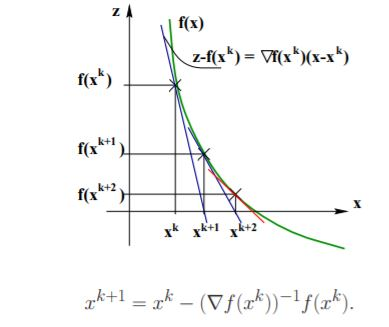
\includegraphics[width=170pt,height=170pt]{newton.jpg}
%    \caption{Demonstracija njutnovog metoda u ravni.}
%    \label{fig:newton}
%\end{figure}
Rješavanje nelinearnih sistema se može generalizovati na funkcije više promjenjivih.\footnote{Za  više informacija pogledati na  \url{http://www.ohiouniversityfaculty.com/youngt/IntNumMeth/lecture13.pdf}.} nPrimijenimo ovu metodu na nalaženje nule funkcije $F(x,y,s)$. Tada imamo
$$ \triangledown F =\left ( \begin{array}{ccc}
	A   & 0      &  0      \\
	0   & A^T    &  I      \\
	S   & 0      & X       \\
\end{array} \right ) 
$$
Prema tome, u fiksnoj tački $(x,y,s)$, Njutnov pravac (pomjeraj)
$
\begin{pmatrix}
	\bigtriangleup  x  \\
	\bigtriangleup  y  \\
	\bigtriangleup  s  \\
\end{pmatrix}
$
%$\bigtriangleup x = x^{k+1} - x^{k}, \bigtriangleup y = y^{k+1} - y^{k}, \bigtriangleup s = s^{k+1} - s^{k}$
se izračunava rješavajući sistem linearnih jednačina

\begin{equation}
	\begin{pmatrix}
		A   & 0      &  0      \\
		0   & A^T    &  I      \\
		S   & 0      & X       \\
	\end{pmatrix}  
	\begin{pmatrix} 
		\bigtriangleup  x  \\
		\bigtriangleup  y  \\
		\bigtriangleup  s  \\
	\end{pmatrix} 
	= 
	\begin{pmatrix} 
		b - Ax             \\
		c - A^T y - s      \\
		- X S \textbf{1}  \\                   
	\end{pmatrix} 
\end{equation}
iz koga se potom računaju tačke naredne  iteracije. 
Njutnov metod   u nekoj iteracija obično narušava uslove nenegativnosti $x,s \geq 0$, ali to se može izbjeći kako će biti  prikazano u nastavku.   
Prethodno   se može lako proširiti i na slučaj kada ne vrijedi $s_ix_i = 0$, ili preciznije kada je $\frac{1}{n}s_ix_i = \mu, \mu > 0$, $i=1,\ldots,n$. Na sličan način računamo Njutnov pravac kada je $s_i x_i \approx \mu \theta$  za  $\theta >0$, iz sistema 

\begin{equation} \label{eq:newton-interior-system-k}    
	\begin{pmatrix}
		A   & 0      &  0      \\
		0   & A^T    &  I      \\
		S   & 0      & X       \\
	\end{pmatrix} 
	\cdot 
	\begin{pmatrix}
		\bigtriangleup  x  \\
		\bigtriangleup  y  \\
		\bigtriangleup  s  \\
	\end{pmatrix} 
	=
	\begin{pmatrix}
		b - Ax           \\
		c - A^T y - s      \\
		\theta \mu \mathbf{1} - X S \textbf{1}                      
	\end{pmatrix}
\end{equation}

%https://www.youtube.com/watch?v=Zf_bn3jJFKY&list=WL&index=9&t=647s
Prema tome, \emph{algoritam unutrašnje tačke} izvršava sljedeće korake:
\begin{enumerate}
	\item Inicijalizujemo $k=0$, te proizvoljno  $(x^k, y^k, s^k), x^k, s^k \geq 0$, $x^k,s^k \in \mathbb{R}^n, y^k \in \mathbb{R}^m$.
	\item Izaberimo $ \theta^k \in [0, 1)$ te riješimo sistem (\ref{eq:newton-interior-system-k}) za $(x^k,y^k,s^k)$ i odabran $\theta = \theta_k$ te $\mu = \mu^k = (y^k)^T s^k $,  odakle   dobijamo
	$  
	\begin{pmatrix}
		\bigtriangleup x^k      \\
		\bigtriangleup y^k       \\
		\bigtriangleup s^k       \\
	\end{pmatrix}    
	$
	
	\item $ 
	\begin{pmatrix}
		x^{k+1}  \\
		y^{k+1}   \\
		s^{k+1}   \\
	\end{pmatrix} \approx
	\begin{pmatrix}
		x^k  \\
		y^k  \\
		s^k  \\
	\end{pmatrix} +   
	\alpha_k 
	\begin{pmatrix}
		\bigtriangleup x^k       \\
		\bigtriangleup y^k       \\
		\bigtriangleup s^k       \\
	\end{pmatrix}  
	$, gdje je $\alpha_k$ izabran na taj način da $(x^{k+1}, s^{k+1}) > 0$, tj. da bi se očuvala dopustivost rješenja. 
	\item Ažurirajmo $k = k + 1$, te se vratimo na korak 2.
\end{enumerate}
Primijetimo da $\mu \rightarrow 0$, kako $k \rightarrow \infty$. U praksi se često stavlja $\theta^k = 1 - \frac{\beta}{n}$, za $\beta \in (0,1)$, a najčešće $\beta= 0.1$.  Parametar $\beta$ upravlja brzinom progresa prema optimalnom rješenju.  


Sljedeća teorema   karakteriše \emph{metod unutrašnje tačke}.

\begin{thm} Za metod unutrašnje tačke vrijedi sljedeće:
	\begin{itemize}
		\item Algoritam unutrašnje tačke konvergira ka optimalnom rješenju problema (\ref{eq:lp_equality_constraint}). %Dualna granica se smanjuje $1 - \frac{\beta}{n}$ pri svakom koraku.
		\item U svim iteracijama, algoritam generiše dopustive tačke.
		\item Kompleksnost algoritma je $O(\sqrt{n})$. %Dakle,  broj iteracija  proporcionalan $\sqrt{n}$ je neophodan  algoritmu unutrašnje tačke riješi problem. 
	\end{itemize}
\end{thm}

Da bi se uvidjele sličnosti i razlike između Simpleks metode i Metode unutrašnje tačke, pogledajte Slike \ref{fig:optimality-approaching-simplex} i  \ref{fig:optimality-approaching-interior}. U njima možete vidjeti kako ova dva metoda pristupaju pretrazi optimalnih rješenja. 

\begin{figure}
	\centering
	\begin{subfigure}{.45\textwidth}
		\centering
		% include first image
		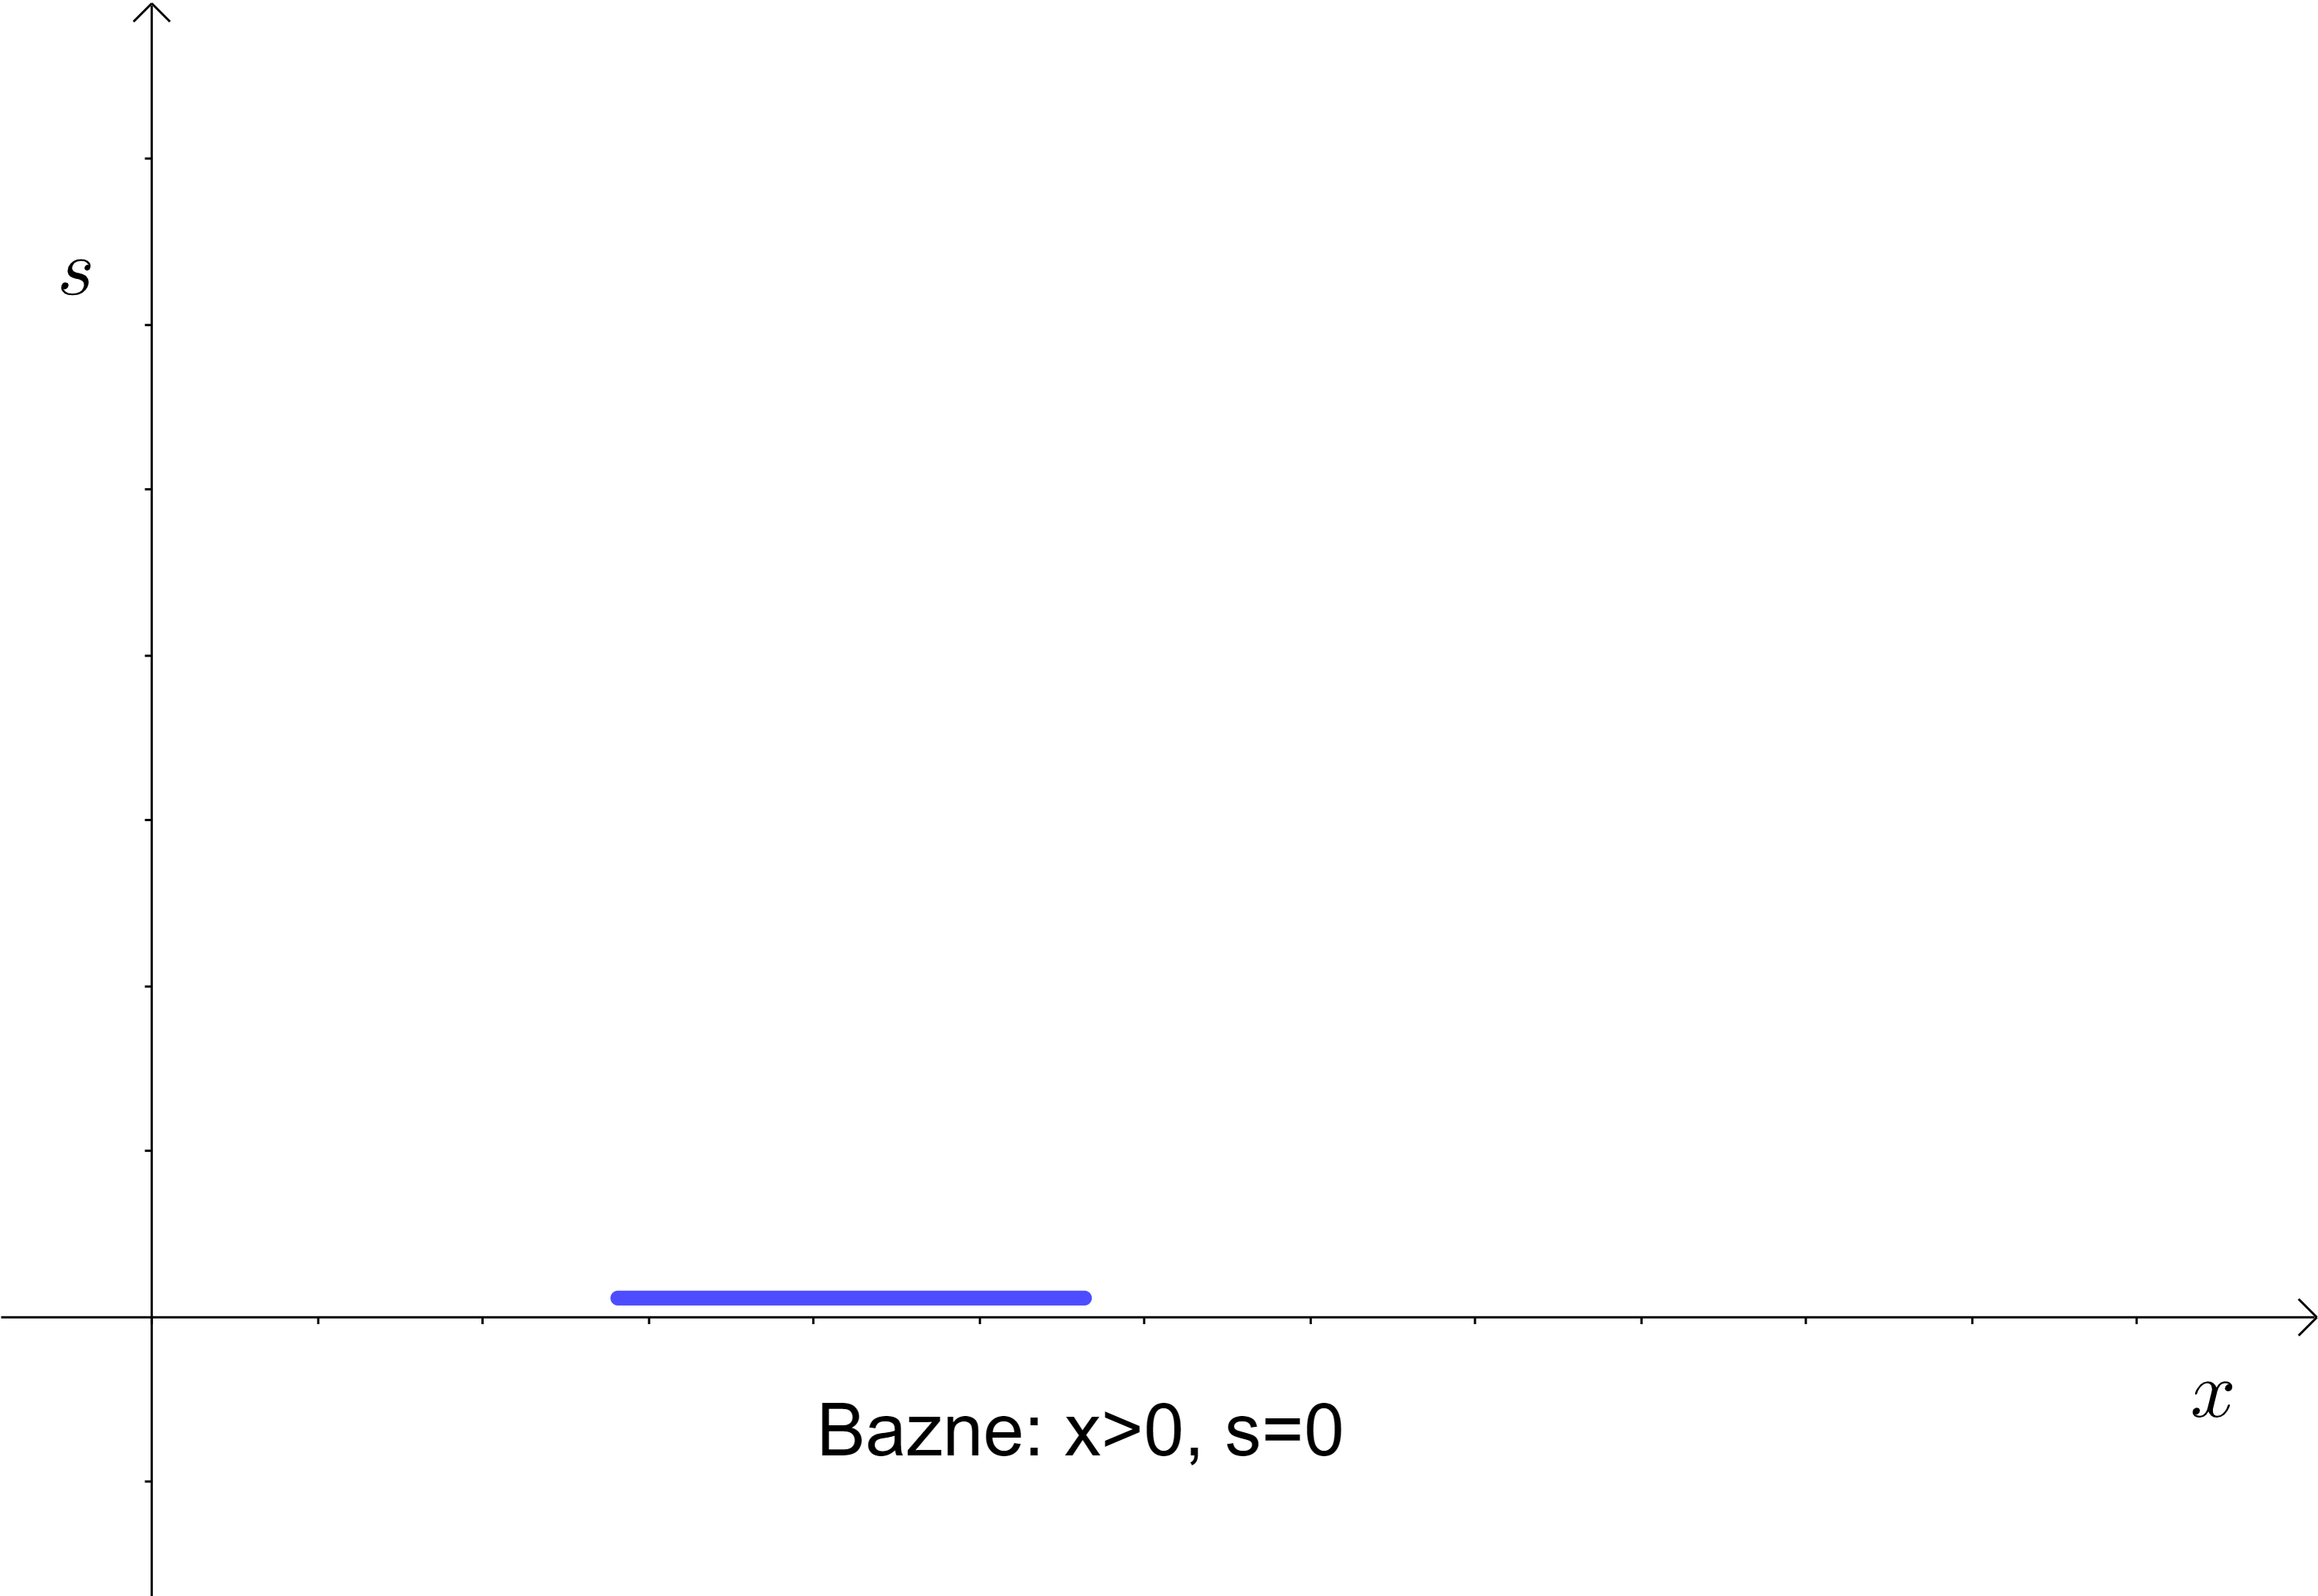
\includegraphics[width=.9\linewidth]{interior-1}  
	\end{subfigure}
	\begin{subfigure}{.45\textwidth}
		\centering
		% include first image
		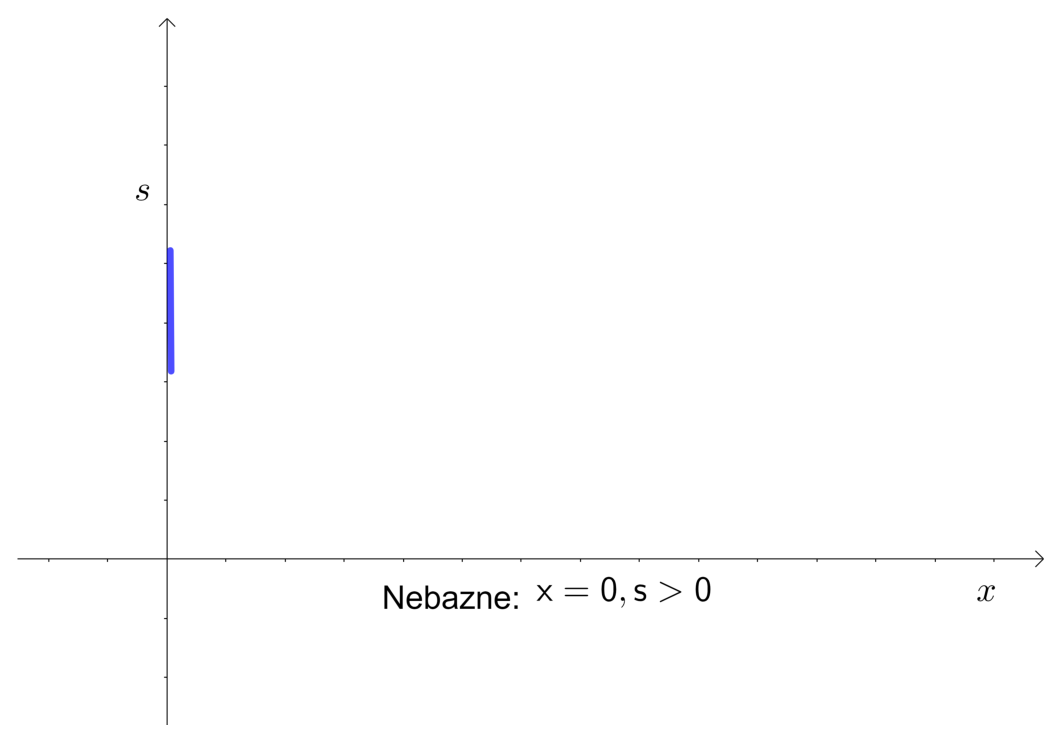
\includegraphics[width=.9\linewidth]{interior-2}  
	\end{subfigure}
	\caption{Prilazak optimalnosti kod Simpleks metode.}
	\label{fig:optimality-approaching-simplex}
\end{figure}


\begin{figure}
	\centering
	\begin{subfigure}{.45\textwidth}
		\centering
		% include first image
		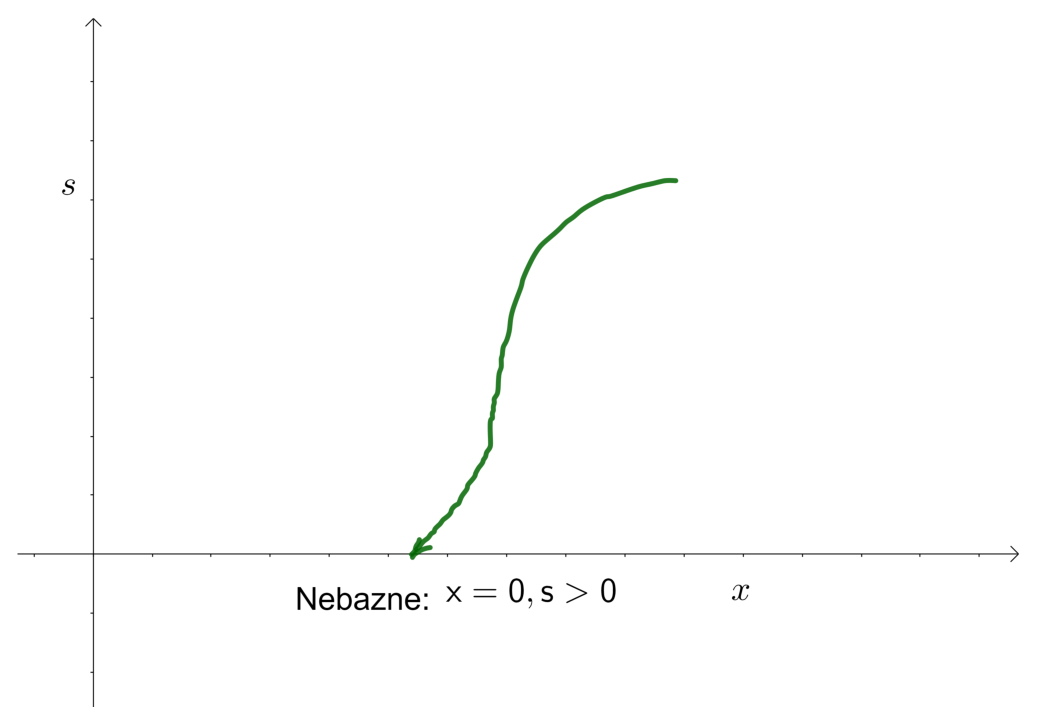
\includegraphics[width=.9\linewidth]{interior-3}  
	\end{subfigure}
	\begin{subfigure}{.45\textwidth}
		\centering
		% include first image
		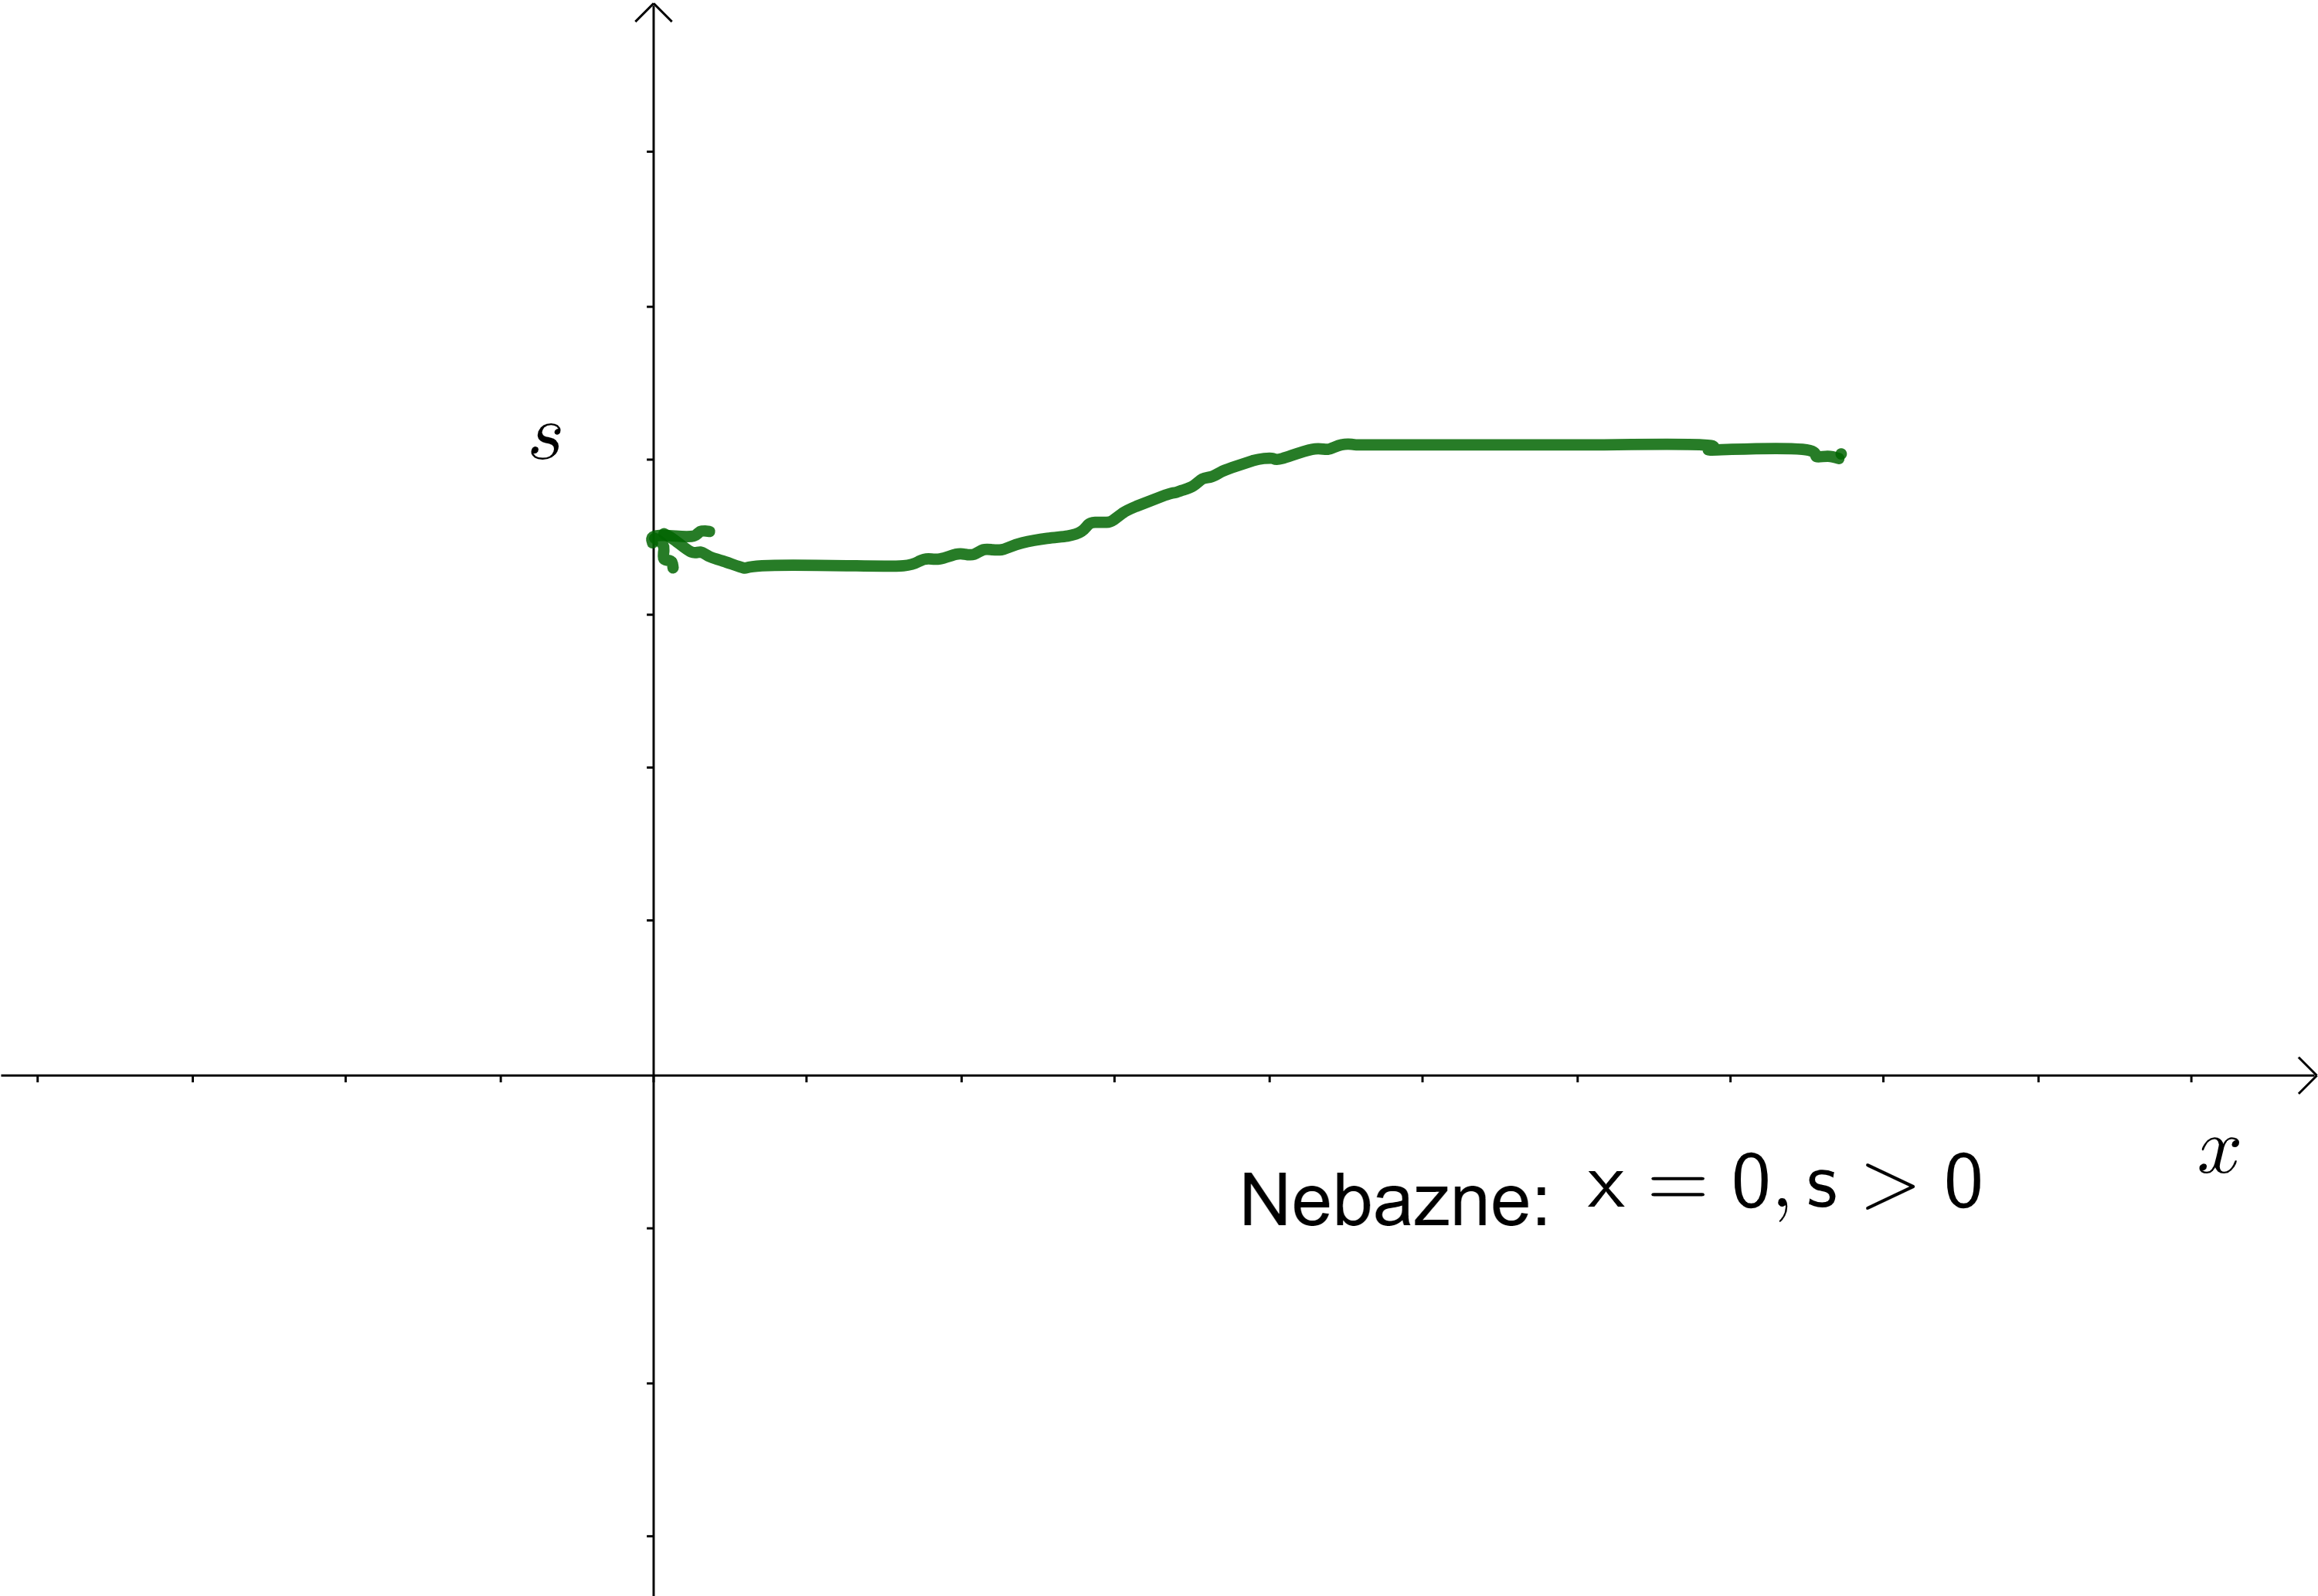
\includegraphics[width=.9\linewidth]{interior-4}  
	\end{subfigure}
	\caption{Prilazak optimalnosti kod Metoda unutrašnje tačke.}
	\label{fig:optimality-approaching-interior}
\end{figure}
Paralelizovani objektno orjentisani optimizacioni siftver baziran na metodi unutrašnje tačke se može naći na 
linku koji je dat pod referencom~\cite{cite_key25}. %\url{https://www.maths.ed.ac.uk/~gondzio/parallel/solver.html}.  \\

%https://optimization.cbe.cornell.edu/index.php?title=Interior-point_method_for_LP
\begin{comment}
	
	\emph{\textbf{Primjer.}} Riješimo sljedeći primjer LP-a pomoću metoda unutrašnje tačke:
	\begin{align*}
		&\max 3 x_1 + 3 x_2 \\
		&\mbox{s.t.} \\
		& x_1 + x_2 \leq 4 \\
		& x_1, x_2 \geq 0.
	\end{align*}
	
	\emph{Rješenje.}  Formirajmo Lagranžovu funkciju početnog problema koristeći ciljnu funkciju barijernog problema sa:  
	\begin{align*}
		L(x, y, \mu) = 	  3 x_1 + 3 x_2 -\mu ln x_1 - \mu ln x_2 + y_1(4- x_1 - x_2 - s_1).  
	\end{align*}
	Barijerna funkcija je uvijek konkavna, a kako maksimizujemo,  tako da posjeduje tačno rješenje.  Sada nađimo maksimum date funkcije što radimo derivirajući funkciju $L$ (nalaženje parcijalnih derivacija):
	\begin{align*}
		&\triangledown_{x_1} L   =  3 - \frac{\mu}{x_1}  - y_1 = 0 \\
		&\triangledown_{x_2} L   =  3 - \frac{\mu}{x_2} - y_1 = 0 \\
		&\triangledown_{y} L   = {4-x_1-x_2 - s_1} = 0 \\
		&\triangledown_{s} L   = { y_1} = 0 
	\end{align*}
	Odakle imamo zbog simetrije prve i druge jednakosti, da je  $x_1 = x_2$, dok je $y(\mu) = 0$. pa prema tome je 
	%$$  3 - \frac{\mu}{x_1}  = 0$$
	%što je ekvivalentno   sa:
	%\begin{align} \label{eq:example-interior-point}
	%   3x_1 - \mu = 0 \Rightarrow x_1 = x_2 = \frac{\mu}{3}.
	%\end{align} 
	Iz trečeg uslova   $x_1(\mu)=x_2(\mu)=2$, što je i optimum. Primijetimo da ovdje nije bilo potrebe za iterativnim postupkom i računanja Njutnovog koraka (koji je konstantan u svim iteracijama). 
	%Kako je ovo kvadratna jednačina, koja je može eksplicitno riješiti, ne treba primjenjivati Njutnov iteracioni postupak (iako bi rješavanje ovakve jednačine takođe bilo moguće pomoću takvog metoda). Dakle, rješenje jednačine (\ref{eq:example-interior-point}) je:
	%\begin{align}
	%	x_1 = \frac{3(4-\mu) \pm \sqrt{9(4-\mu)^2 - 96 \mu}} { 12} = x_2
	%\end{align}
	% dualni simpleks metod ==> 4.7 PRIMAL-DUAL ALGORITHMS
	% Ako bi uzeli $\mu = 1$, rješenje koje se dobije je 
\end{comment}

\chapter{Makefile za kompajliranje \textsc{Cplex} programa}\label{appendix:makefile-cplex}

\begin{center}
	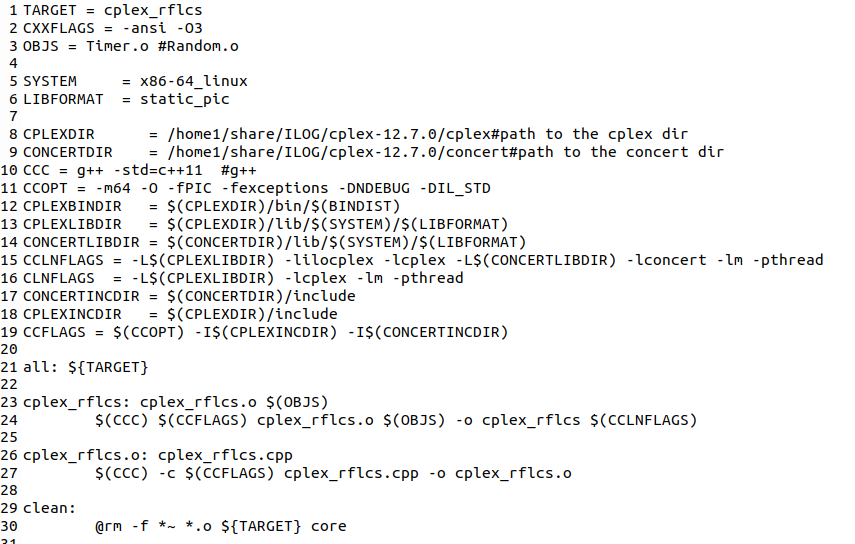
\includegraphics[width=420pt,height=300pt]{cplex_makefile.png}
\end{center}

Za pokretanje progama uz pomoć $makefile$ datoteke (komande $make$), potrebno je pratiti sljedeće korake. 
\begin{itemize}
	\item Instalirati  C++, sa kompajlerom GCC (verzija 9, recimo).
	\item Intalirati je \textsc{Cplex}. 
	\item U promjenljivim CPLEXDIR i CONCERTDIR (linije 8 i 9), poresiti putanje ka cplex i concert direktorijumima, redom.
	\item Napisati program cplex\_rfrcs.cpp i dodatni .cpp za mjerenje vremena izvršavanja algoritma, nazvan Timer.cpp. (Pisanje Timer.cpp nije obavezno. U tom slučaju sadržaj promjenljive OBJS na liniji 3 je prazan.)
\end{itemize}

\begin{thebibliography}{widest entry}
	\bibitem[1]{cite_key1} M. Leila, The big picture of Operations Research, preuzeto 24.7.2022. \url{https://towardsdatascience.com/the-big-picture-of-operations-research-8652d5153aad}
	\bibitem[2]{cite_key2} Hillier, Frederick S. Introduction to operations research. Tata McGraw-Hill Education, 2012.
	\bibitem[3]{cite_key3} M. Lavrov, Linear programming, skripta, preuzeto 24.7.2022. \url{https://faculty.math.illinois.edu/~mlavrov/}
	 \bibitem[4]{cite_key4}  Bisschop, Johannes. AIMMS optimization modeling. Lulu. com, 2006.
	  \bibitem[5]{cite_key5} Feillet, Dominique. ,,A tutorial on column generation and branch-and-price for vehicle routing problems.'' 4or 8.4 (2010): 407-424.
	  \bibitem[6]{cite_key6}  Rebeka Čordaš. Linearno programiranje i primjene. Sveu\v cili\v ste J.J.Strossmayera u Osijeku, diplomski rad (2012)
	  \bibitem[7]{cite_key7}   Manual, \textsc{Cplex} User’S. ,,Ibm ilog cplex optimization studio.'' Version 12 (1987): 1987-2018.
	  \bibitem[8]{cite_key8} Mitchell, Stuart, Michael OSullivan, and Iain Dunning. "PuLP: a linear programming toolkit for python." The University of Auckland, Auckland, New Zealand (2011): 65.
	  \bibitem[9]{cite_key9}    Talbi, El-Ghazali. Metaheuristics: from design to implementation. Vol. 74. John Wiley \& Sons, 2009.
	  \bibitem[10]{cite_key10}     Vazirani, Vijay V. Approximation algorithms. Springer Science \& Business Media, 2013.
	   \bibitem[11]{cite_key11}     Blum, Christian, Maria J. Blesa, and Manuel Lopez-Ibanez. ,,Beam search for the longest common subsequence problem.'' Computers \& Operations Research 36.12 (2009): 3178-3186.
	 % Odjel za matematiku
	   \bibitem[12]{cite_key12}   Raidl, Günther R., and Jakob Puchinger. ,,Combining (integer) linear programming techniques and metaheuristics for combinatorial optimization.'' Hybrid metaheuristics (2008): 31-62.
	     \bibitem[13]{cite_key13}      Rahmaniani, Ragheb, et al. "The Benders decomposition algorithm: A literature review." European Journal of Operational Research 259.3 (2017): 801--817.
	     \bibitem[14]{cite_key14}    Raidl, Günther R. ,,Decomposition based hybrid metaheuristics.'' European journal of operational research 244.1 (2015): 66-76.
	      \bibitem[15]{cite_key15}  Mladenović, N., and  Hansen P. ,,Variable neighborhood search.'' Computers \& Operations Research 24.11 (1997): 1097-1100.
	      \bibitem[16]{cite_key15} CPLEX User Manual, preuzeto 24.7.2022. \url{https://www.tu-chemnitz.de/mathematik/discrete/manuals/cplex/doc/userman/html/cpxUserAppendixA.html}
	      \bibitem[17]{cite_key17}Mitchell, S., OSullivan, M., and Dunning, I. (2011). PuLP: a linear programming toolkit for python. The University of Auckland, Auckland, New Zealand, 65.
	      \bibitem[18]{cite_key18}S. A. Mitchell and J.S. Roy. PuLP. PuLP Case Studies. preuzeto 24.7.2022. \url{https://www.coin-or.org/PuLP/CaseStudies/index.html}
	      \bibitem[19]{cite_key19} S. A. Mitchell and J.S. Roy. PuLP. preuzeto 24.7.2022. \url{ http://www.coin-or.org/PuLP/.}
          \bibitem[20]{cite_key20}Sergiy Butenko, Dantzig-Wolfe Decomposition for LPs with Block Diagonal Structure: An Example, Nov 17, 2020. YouTube  \url{https://www.youtube.com/watch?v=wxz0NJvKZNM}
           \bibitem[21]{cite_key21} Sergiy Butenko, Dantzig-Wolfe Decomposition: Intro, Nov 10, 2020. YouTube \url{https://www.youtube.com/watch?v=IposxYVBUnY}
            \bibitem[22]{cite_key22} Shahidehpour, Mohammad, and Yong Fu. "Benders decomposition in restructured power systems." IEEE Techtorial April (2005). \url{http://motor.ece.iit.edu/ms/benders.pdf}
            \bibitem[23]{cite_key23} S.Sankaranarayanan, Integer Linear Programming, skripta, preuzeto 24.7.2022. \url{https://home.cs.colorado.edu/\~srirams/courses/csci5654-fall13/ilpLectures.pdf}
  \bibitem[24]{cite_key24} Cplex II. V12. 1: User’s Manual for CPLEX. International Business Machines Corporation. 2009;46(53):157. \url{https://www.ibm.com/products/ilog-cplex-optimization-studio}
  
   \bibitem[25]{cite_key25} Jacek Gondzio, Exploiting Structure with Interior Point Method, preuzeto 24.7.2022.   \url{https://www.maths.ed.ac.uk/~gondzio/parallel/solver.html}
   
    \bibitem[26]{cite_key26} John E. Mitchell, Gomory Cutting Planes, skripta, preuzeto 24.7.2022. \url{https://homepages.rpi.edu/~mitchj/handouts/gomorycuts/gomorycuts.html}
   \bibitem[27]{cite_key27}  Williamson, David P., and David B. Shmoys. ,,The design of approximation algorithms.'' Cambridge university press, 2011.
    \bibitem[28]{cite_key28} Adi, Said S., et al. ,,Repetition-free longest common subsequence.'' Discrete Applied Mathematics 158.12 (2010): 1315--1324.
     \bibitem[29]{cite_key29}  Cornuéjols, Gérard, George Nemhauser, and Laurence Wolsey. ,,The uncapicitated facility location problem.'' Cornell University Operations Research and Industrial Engineering, 1983.
    \bibitem[30]{cite_key30} Asghari, M., Fathollahi-Fard, A. M., Mirzapour Al-e-hashem, S. M. J., \& Dulebenets, M. A. (2022). Transformation and Linearization Techniques in Optimization: A State-of-the-Art Survey. Mathematics, 10(2), 283.
    \bibitem[31]{cite_key31} Lozano, L., Medaglia, A. L. (2013). On an exact method for the constrained shortest path problem. Computers \& Operations Research, 40(1), 378-384.
    \bibitem[32]{cite_key32} Jovanović, M. (2013): Konveksne funkcije i ekstremi, Prirodno-matematički fakultet, Univerzitet u Banjoj Luci.
    \bibitem[33]{cite_key33} Dugošija, Đ., Savić, A. (2018). Operaciona istraživanja: linearno i celobrojno programiranje, grafovi i algoritmi (1. izd.). Matematički fakultet.
    \bibitem[34]{cite_key34} Čangalović, M., Dugošija, Đ., Kovačević-Vujčić, V., Simić, S., \& Vuleta, J. (1996). Kombinatorna optimizacija: matematička teorija i algoritmi.
\end{thebibliography}

\end{document}
 